
\chapter{ಸಾಮಾಜಿಕ ಸಂಸ್ಕೃತಿ}

ಸಾಮಾಜಿಕವಾಗಿ ಸಾಂಸ್ಕೃತಿಕವಾಗಿ ಕನ್ನಡ ನಾಡವರು ಅಂದರೆ ನಾಡಿನ ಜನರು ಅಥವಾ ಜನಪದರು...

\section{ವೀರಗಲ್ಲು/ಮಾಸ್ತಿಕಲ್ಲು/ವೇಳೆವಾಳಿ/ನಿಸಿದಿಗಲ್ಲು}

ಹುಟ್ಟಿದವನು ಸಾಯಲೇ ಬೇಕು, ಮರಣದ ನಂತರ ಸದ್ಗತಿ ಅಥವಾ ಮೋಕ್ಷ. ಆದರೆ ಬದುಕಿರುವಷ್ಟು ಕಾಲ ಉನ್ನತ ಧ್ಯೇಯ ಆದರ್ಶಗಳನ್ನು ಇಟ್ಟುಕೊಂಡು, ಅದಕ್ಕಾಗಿ ಬದುಕಬೇಕು, ಆ ಮೌಲ್ಯಗಳ ರಕ್ಷಣೆಗಾಗಿಯೇ ಜೀವನವನ್ನು ಸವೆಸಬೇಕು, ಅದಕ್ಕಾಗಿಯೇ ಹೋರಾಡಿ ಸಾಯಬೇಕು, ಅದರಿಂದಲೇ ಮುಕ್ತಿ. ಇದು ನಮ್ಮ ಭಾರತೀಯ ಸಂಸ್ಕೃತಿಯಲ್ಲಿ ಮನುಷ್ಯ ತನ್ನ ಜೀವನದ ಬಗ್ಗೆ ಹೊಂದಿದ್ದ ಒಂದು ತತ್ವ ಅಥವಾ ಸಿದ್ಧಾಂತ. ಆದುದರಿಂದ ಲೌಕಿಕವನ್ನೇ ಪ್ರಧಾನವಾಗಿ ಅನುಸರಿಸುವ ಜನರು ಅವರ ಬದುಕಿನ ಕಾಲದ ಉದ್ದಕ್ಕೂ ಅವರು ನಂಬಿದ ಉನ್ನತ ಧ್ಯೇಯ, ಆದರ್ಶ, ಮೌಲ್ಯಗಳಿಗಾಗಿ ಬದುಕುತ್ತಿದ್ದರು. ಅದಕ್ಕಾಗಿ ಹೋರಾಡಿ ಮಡಿಯುತ್ತಿದ್ದರು. ಇವರ ನೆನಪಿನ ಸ್ಮಾರಕಗಳೇ ವೀರಮರಣ ಸ್ಮಾರಕಗಳು. ಧಾರ್ಮಿಕ ಜೀವನಕ್ಕೆ ಮಹತ್ವ ನೀಡಿದವರು ವ್ರತ ಉಪವಾಸ ಮುಂತಾದ ಧಾರ್ಮಿಕ ಆಚರಣೆಗಳ ಮೂಲಕ ತಮ್ಮ ಜೀವವನ್ನು ಕೊನೆಗಾಣಿಸಿಕೊಳ್ಳುತ್ತಿದ್ದರು. ಇವೇ ಧಾರ್ಮಿಕ ಆತ್ಮಬಲಿದಾನ ಸ್ಮಾರಕಗಳು. ಇಂತಹ ಆದರ್ಶ ಪುರುಷರು ಮೌಲ್ಯಗಳ ರಕ್ಷಣೆಯಲ್ಲಿ, ಮೌಲ್ಯಗಳ ಅನುಷ್ಠಾನದಲ್ಲಿ ಜೀವವನ್ನು ಕೊನೆಗಾಣಿಸಿಕೊಂಡಾಗ, ಜನತೆ ಅವರು ಮಾಡಿದ ಕಾರ್ಯವನ್ನು ಉಲ್ಲೇಖಿಸಿ ಅಥವಾ ವರ್ಣಿಸಿ ಅವರ ನೆನಪಿಗಾಗಿ ಸ್ಮಾರಕಗಳನ್ನು ನಿಲ್ಲಿಸುತ್ತಿದ್ದರು. ಇವೇ ಸ್ಮಾರಕ ಶಿಲೆಗಳು.

ಮಂಡ್ಯ ಜಿಲ್ಲೆಯಲ್ಲಿ ಈ ಬಗೆಯ ಸ್ಮಾರಕ ಶಿಲೆಗಳಾದ, ವೀರಗಲ್ಲು, ಮಾಸ್ತಿಕಲ್ಲು, ಲೌಕಿಕ ಆತ್ಮ ಬಲಿದಾನಕ್ಕೆ ಸಂಬಂಧಿಸಿದ ಗರುಡರ ಶಾಸನಗಳು, ಹಿಂದೂ ಧಾರ್ಮಿಕ ಆತ್ಮ ಬಲಿದಾನಕ್ಕೆ ಸಂಬಂಧಿಸಿದ ಮಾಸ್ತಿಕಲ್ಲುಗಳು, ಜೈನ ಧಾರ್ಮಿಕ ಆತ್ಮ ಬಲಿದಾನಕ್ಕೆ ಸಂಬಂಧಿಸಿದ ನಿಸಿದಿಗಲ್ಲುಗಳು ಅಪಾರ ಸಂಖ್ಯೆಯಲ್ಲಿವೆ.


\section{ವೀರಗಲ್ಲುಗಳು}

ಪ್ರಾಚೀನ ಕಾಲದಲ್ಲಿ ಪ್ರತಿಯೊಂದು ಗ್ರಾಮಗಳಲ್ಲಿಯೂ ಊರಿನ ಒಡೆಯರಾದ ಗಾವುಂಡರು, ಅವರ ವಂಶದವರು, ಅವರ ಅನುಯಾಯಿಗಳು, ಊರು, ಪ್ರಜೆ, ಮುಂತಾದ ಗ್ರಾಮದ ಸಂಘಗಳ ಸದಸ್ಯರು, ಜನಸಾಮಾನ್ಯರ ವೀರರ ತಂಡಗಳು ಊರಿನ ರಕ್ಷಣೆಗೆ, ಗಡಿಯ ರಕ್ಷಣೆಗೆ, ತುರುಗಳ ರಕ್ಷಣೆಗೆ, ಹೆಣ್ಣಿನ ಮಾನ ಕಾಪಾಡಲು, ಪ್ರಾಣದ ಹಂಗು ತೊರೆದು ಹೋರಾಡಲು ಸಿದ್ಧರಾಗಿರುತ್ತಿದ್ದರು. “ಆ ಕಾಲದಲ್ಲಿ ಈಗಿನಂತೆ ದೇಶದ ನಾನಾ ಭಾಗಗಳಲ್ಲಿ ಆಡಳಿತವರ್ಗದಿಂದ ನೇಮಿತವಾದ ರಕ್ಷಣಾ ವ್ಯವಸ್ಥೆಯಿರಲಿಲ್ಲ. ಒಂದೊಂದು ಗ್ರಾಮದಲ್ಲೂ ಅದರ ರಕ್ಷಣೆಗಾಗಿ ಆ ಊರಿನ ಒಂದು ವೀರರ ತಂಡವೇ ಸಿದ್ಧವಾಗಿರುತ್ತಿತ್ತು, ಇಡೀ ವಾತಾವರಣವೇ ಕ್ಷಾತ್ರತೇಜಸ್ಸಿನಿಂದ ತುಂಬಿ ತುಳುಕುತ್ತಿತ್ತು.\endnote{ ಚಿದಾನಂದಮೂರ್ತಿ, ಡಾ॥ ಎಂ. ಕನ್ನಡ ಶಾಸನಗಳ ಸಾಂಸ್ಕೃತಿಕ ಅಧ್ಯಯನ, ಪುಟ 248} “ಉದಾತ್ತವಾದ ಉದ್ದೇಶದಿಂದ ಯುದ್ಧದಲ್ಲಿ ಹೋರಾಡಿ ಮಡಿದ ವೀರರ ಸ್ಮಾರಕವಾಗಿ ನಿಲ್ಲಿಸುವ ಕಲ್ಲುಗಳೇ ವೀರಗಲ್ಲುಗಳು”\endnote{ ಪೂರ್ವೋಕ್ತ - ಪುಟ251} “ಹಿಂದೂ ಬಲಿದಾನ ಮರಣ ಮತ್ತು ಹಿಂದೂ ವೀರಮರಣಗಳ ನೆನಪನ್ನು ಹೊತ್ತು ನಿಂತುವೇ ಮರಣ ಸ್ಮಾರಕಗಳು”, “ವೀರಜೀವನವನ್ನು ಪ್ರತಿಪಾದಿಸಲು ವಿಕ್ರಮಾರ್ಜುನ ವಿಜಯ, ಸಾಹಸಭೀಮವಿಜಯಗಳಂತಹ ಕೃತಿಗಳೂ, ವೀರಘಟನೆಗಳನ್ನು ಪ್ರತಿನಿಧಿಸಲು ಸಾವಿರಾರು ವೀರಗಲ್ಲುಗಳೂ ನಾಡಿನ ತುಂಬ ತಲೆಯೆತ್ತಿ ನಿಂತವು”, “ಕರ್ನಾಟಕದಲ್ಲಿ ಈ ವೀರಸ್ತೋಮ ಮೂರು ವಿಧವಾಗಿದ್ದಿತು, ಒಂದು: ಗ್ರಾಮದ ಪ್ರಜಾಸಮೂಹ, ಎರಡು: ಗ್ರಾಮದ ಕಾಯ್ದಿಟ್ಟ ಪಡೆ, ಮೂರು:ರಾಜನ ಸೈನ್ಯಪಡೆ”.\endnote{ ಕಲಬುರ್ಗಿ ಡಾ॥ ಎಂ.ಎಂ., ಸಮಾಧಿ-ಬಲಿದಾನ-ವೀರಮರಣಸ್ಮಾರಕಗಳು, ಪುಟ 70-74} “ಶತ್ರುಗಳೊಡನೆ ಹೋರಾಡಿ ಸತ್ತ ವೀರರ ನೆನಪಿನಲ್ಲಿ ಹಾಕಿಸಿರುವ ಕಲ್ಲುಗಳೇ ವೀರಗಲ್ಲುಗಳು”.\endnote{ ದೇವರಕೊಂಡಾರೆಡ್ಡಿ, ಡಾ॥, ಕರ್ನಾಟಕದ ಶಾಸನಗಳು, ಪುಟ 18} “ವೀರಗಲ್ಲು, ನಿಷಿಧಿಗಲ್ಲು, ಮಾಸ್ತಿಗಲ್ಲು, ಇವುಗಳೆಲ್ಲವೂ ಸ್ಮಾರಕಶಿಲೆಗಳು. ಕದನಗಳಲ್ಲಿ, ತುರುಗಾಳಗದಲ್ಲಿ, ಗ್ರಾಮದ ದರೋಡೆಯ ಸಂದರ್ಭಗಳಲ್ಲಿ, ಸೀಮಾಸಂಬಂಧವಾದ ಜಗಳಗಳಲ್ಲಿ ಮಡಿದವರ ನೆನಪಿಗಾಗಿ ಹಿಂದೆ ವೀರಗಲ್ಲುಗಳನ್ನು ನೆಡಿಸುವುದು ಕರ್ನಾಟಕದಲ್ಲಿ ಕಂಡುಬಂದ ವಿಶಿಷ್ಟಪದ್ಧತಿ, ಇಂತಹ ವೀರಗಲ್ಲುಗಳು ಕರ್ನಾಟಕದಲ್ಲಿ ಸಿಗುವಷ್ಟು ಸಂಖ್ಯೆಯಲ್ಲಿ ಬೇರಾವ ರಾಜ್ಯಗಳಲ್ಲಿಯೂ ಕಂಡುಬರುವುದಿಲ್ಲ”.\endnote{ ಗೋಪಾಲ್​ ಡಾ॥ ಬಾ.ರಾ., ಕನ್ನಡ ಶಾಸನಗಳು, ಕನ್ನಡ ಸಾಹಿತ್ಯ ಪರಿಷತ್ತು, ಪುಟ 30-31} “ಆತ್ಮ ಬಲಿದಾನ ಗೆಯ್ದವರ ಸ್ಮಾರಕವಾಗಿ ನಿಲ್ಲಿಸುವ ಶಿಲೆಗಳಿಗೆ ಆತ್ಮ ಬಲಿದಾನ ಸ್ಮಾರಕಗಳೆಂದು, ವೀರಮರಣ ಹೊಂದಿದವರ ಸ್ಮಾರಕವಾಗಿ ನಿಲ್ಲಿಸಿದ ಶಿಲೆಗಳಿಗೆ ವೀರಗಲ್ಲುಗಳೆಂದೂ ಹೆಸರು” ಈ ಕ್ಷೇತ್ರದಲ್ಲಿ ವಿಶೇಷ ಅಧ್ಯಯನ ಮಾಡಿರುವ ವಿದ್ವಾಂಸರ ಅಭಿಪ್ರಾಯಗಳಾಗಿವೆ..\endnote{ ಹಿರೇಮಠ್​, ಡಾ॥ ಬಿ.ಆರ್​., ವೀರಗಲ್ಲುಗಳು, ಕರ್ನಾಟಕ ವಿವಿ. ಪುಟ 4-5}

ಕರ್ನಾಟಕದ ವೀರಗಲ್ಲುಗಳನ್ನು ಎರಡು ರೀತಿಗಳಲ್ಲಿ ವಿಂಗಡಿಸಲಾಗಿದೆ. (1) ಹೋರಾಟದಲ್ಲಿ ಅರಸನ ಪರವಾಗಿಯೋ ಊರಿನ ಹಿತರಕ್ಷಣೆಗಾಗಿಯೋ ಹೋರಾಡಿ ಶತ್ರುವಿನಿಂದ ಮಡಿದ ವೀರರ ಸ್ಮಾರಕ ಶಿಲೆಗಳು. (2) ಅರಸನ ಪರವಾಗಿಯೋ, ಊರಿನ ಹಿತದೃಷ್ಟಿಯಿಂದಲೋ, ವೈಯಕ್ತಿಕ ಮೋಕ್ಷಾಪೇಕ್ಷೆಯ ದೃಷ್ಟಿಯಿಂದಲೋ ಹಿಂಸಾತ್ಮಕವಾದ ರೀತಿಯಲ್ಲಿ ಆತ್ಮಬಲಿಯನ್ನು ಮಾಡಿಕೊಂಡು ಮಡಿದ ವೀರರ ಸ್ಮಾರಕ ಶಿಲೆಗಳು.\endnote{ ಶೇಷಶಾಸ್ತ್ರಿ ಡಾ॥ ಆರ್​., ಕರ್ನಾಟಕದ ವೀರಗಲ್ಲುಗಳು, ಪುಟ 42-43}

“ಈ ಪ್ರಸಂಗಗಳಲ್ಲದೆ ಕಳ್ಳರನ್ನು ಎದುರಿಸಿ ಸತ್ತವರ, ಕ್ರೂರಪ್ರಾಣಿಗಳನ್ನು ಬೇಟೆಯಾಡುತ್ತಾ ಸತ್ತವರ ವೀರಗಲ್ಲುಗಳೂ ಸಿಗುತ್ತವೆ, ಇದಲ್ಲದೆ ಪರಸ್ಪರ ಹೋರಾಟದಲ್ಲಿ, ಸತ್ತ ಪ್ರಾಣಿಗಳ ಸ್ಮಾರಕವಾಗಿಯೂ ನಿಲ್ಲಿಸಿದ ವೀರಗಲ್ಲುಗಳು ಸಿಗುವುದುಂಟು”.\endnote{ ಕಲಬುರ್ಗಿ, ಡಾ॥ ಎಂ.ಎಂ., ಸಮಾಧಿ-ಬಲಿದಾನ-ವೀರಮರಣ ಸ್ಮಾರಕಗಳು, ಪುಟ 83} ವೀರಗಲ್ಲುಗಳನ್ನು ಡಾ.ಶೇಷಶಾಸ್ತ್ರಿಯವರು ಈ ಕೆಳಗಿನಂತೆ ವಿಂಗಡಿಸುತ್ತಾರೆ.\endnote{ ಶೇಷಶಾಸ್ತ್ರಿ, ಡಾ॥ ಆರ್​, ಪೂರ್ವೋಕ್ತ, ಪುಟ 113-14} 1)ಕಳ್ಳರೊಡನೆ ಹೋರಾಡಿ ಮಡಿದ ವೀರರು 2)ಪೆಣ್ಬುಯ್ಯಲಿನಲ್ಲಿ ಮಡಿದ ವೀರರು 3)ಸೀಮಾಸಂಬಂಧದ ಕಾಳಗದಲ್ಲಿ ಮಡಿದ ವೀರರು 4)ಊರಳಿವು-ಊರ ಹುಯ್ಯಲಿನಲ್ಲಿ ಸತ್ತವೀರರು 5)ನೀರಲ್ಲಿ ಸತ್ತ ವೀರರು 6) ಬೇಟೆಯಲ್ಲಿ ಸತ್ತವೀರರು 7)ತುರುಗಾಳಗದಲ್ಲಿ ಸತ್ತವೀರರು 8)ಯುದ್ಧದಲ್ಲಿ ಸತ್ತ ವೀರರು.

ಪ್ರಾಚೀನ ಕಾಲದಲ್ಲಿ ವೀರಗಲ್ಲುಗಳಿಗೆ “ಕಲ್ಲು” ಎಂಬ ಪ್ರಯೋಗವನ್ನು ಹೆಚ್ಚಾಗಿ ಮಾಡಿದೆ. ನಂತರ \textbf{‘ವೀರಸಾಸನ’} ಮತ್ತು ‘ವೀರಗಲ್ಲು’. ‘ವೀರಕಲ್ಲು’. ‘ಬೀರಕಲ್ಲು’ ಎಂಬ ಪದಗಳು ಪ್ರಯೋಗವಾಗಿರುವುದು ತಿಳಿದುಬರುತ್ತದೆ.\endnote{ ಶೇಷಶಾಸ್ತ್ರಿ, ಡಾ॥ ಆರ್​. ಪೂರ್ವೋಕ್ತ, ಪುಟ 94-96} ಮಂಡ್ಯ ಜಿಲ್ಲೆಯ ಶಾಸನಗಳಲ್ಲಿ, \textbf{ಸಸನ(ಶಾಸನ)}\endnote{ ಎಕ 6 ಕೃಪೇ 15 ಕರತಾಳ(ಬೇಚರಾಕ್​) 11ನೇ ಶ.}, \textbf{ಕಲ್ಲು}\endnote{ ಎಕ 6 ಕೃಪೇ 19 ಆಲೇನಹಳ್ಳಿ 9ನೇ ಶ., ಎಕ 7 ನಾಮಂ 175 ಮಡಕೆಹೊಸೂರು 10ನೇ ಶ., ನಾಮಂ 137 ಬೇಗಮಂಗಲ 11ನೇ ಶ.

ಎಕ 6 ಕೃಪೇ 17 ಮಂಚಿಬೀಡು 11ನೇ ಶ. ಎಕ 7 ಮವ 28 ಹುಲ್ಲಹಳ್ಳಿ 1171,

ಎಕ 7 ಮವ 128 ಕದವಳ್ಳಿ 1183, ಮ 120 ಕಡ್ಲವಾಗಿಲು1192, ಕೃಪೇ 67 ನಾಯಕನಹಳ್ಳಿ 12ನೇ ಶ., ಕೃಪೆ 70 ಕೈಗೋನಹಳ್ಳಿ 12ನೇ ಶ.}, \textbf{ವೀರಸಾಸನ}\endnote{ ಎಕ 7 ಮ 112 ಬೊಪ್ಪಸಂದ್ರ 1175, ಕೃಪೇ 78 ಅಗ್ರಹಾರಬಾಚಹಳ್ಳಿ 1224, ಕೃಪೇ 79 ಅಗ್ರಹಾರಬಾಚಹಳ್ಳಿ 1242}, \textbf{ಬೀರಗಲ್ಲು, ವೀರಗಲ್ಲು, ವೀರಕಲ್ಲು}\endnote{ ಎಕ 7 ನಾಮಂ 106 ಹೊನ್ನೇನಹಳ್ಳಿ 1180, ನಾಮಂ 109 ಚುಂಚನಹಳ್ಳಿ 13ನೇ ಶ. ನಾಮಂ 6 ನಾಮಂ 1204, ನಾಮಂ 111 ಚುಂಚನಹಳ್ಳಿ 1205, ಎಕ 7 ಮವ 36 ಹುಲ್ಲೇಗಾಲ 1219, ಮ 97 ಬೆಲ್ಲೂರು 1264, ಮ 101 ಕಡ್ಲವಾಗಿಲು 1285,

ಮವ 27 ಹುಲ್ಲಹಳ್ಳಿ 1387, ಮ 79 ಹಾಗಲಹಳ್ಳಿ 1387, ಎಕ 7 ಮ 119 ಕಡ್ಲವಾಗಿಲು 13ನೇ ಶ. ಮ 114 ಬೊಪ್ಪಸಂದ್ರ 14ನೇ ಶ.} ಎಂಬ ಪ್ರಾಚೀನ ಪ್ರಯೋಗಗಳು ದೊರೆಯುತ್ತವೆ. ಬರಹ ಇರುವ ವೀರಗಲ್ಲುಗಳನ್ನು ವೀರಶಾಸನ ಎಂದೂ, ಬರಹವಿಲ್ಲದ ವೀರರ ಸ್ಮಾರಕಗಳನ್ನು ವೀರಗಲ್ಲುಗಳೆಂದು ಹೇಳಬಹುದು. ಪಂಪ ಮಹಾಕವಿಯೂ ಬೀರ ಶಾಸನ ಎಂಬ ಪದ ಪ್ರಯೋಗ ಮಾಡಿದ್ದಾನೆ.\endnote{ ಪಂಪ ಮಹಾಕವಿಯ ವಿಕ್ರಮಾರ್ಜುನ ವಿಜಯ ಆಶ್ವಾಸ 14, ಪದ್ಯ 56.}

ಮಂಡ್ಯ ಜಿಲ್ಲೆಯಲ್ಲಿ ಬಹು ಸಂಖ್ಯೆಯಲ್ಲಿ ವೀರರಗುಡಿ, ಮಾಸ್ತಿಗುಡಿಗಳಿರುವುದನ್ನು, ಬಹಳ ಕಾಲದ ಹಿಂದೆಯೇ, ಡಾ. ಚಿದಾನಂದಮೂರ್ತಿಯವರು,\endnote{ ಚಿದಾನಂದಮೂರ್ತಿ ಡಾ॥ ಎಂ., ಪೂರ್ವೋಕ್ತ - ಪುಟ251} ಆರ್​.ಶೇಷಶಾಸ್ತ್ರಿಯವರು ಗುರುತಿಸಿದ್ದಾರೆ.\endnote{ ಶೇಷಶಾಸ್ತ್ರಿ ಡಾ॥ ಆರ್​. ಕರ್ನಾಟಕದ ವೀರಗಲ್ಲುಗಳು, ಪುಟ63} ಇದರಿಂದ ಮಂಡ್ಯ ಜಿಲ್ಲೆಯು ವೀರರ ನಾಡಾಗಿತ್ತೆಂದು ಹೇಳಬಹುದು. ಜಿಲ್ಲೆಯಲ್ಲಿ ಬರಹವಿಲ್ಲದ ವೀರಗಲ್ಲುಗಳು, ಮಾಸ್ತಿಕಲ್ಲುಗಳ ಸಂಖ್ಯೆ ಹೆಚ್ಚು. ಜಿಲ್ಲೆಯ ಅನೇಕ ಊರುಗಳಲ್ಲಿ ಬರಹವಿಲ್ಲದ ವೀರಗಲ್ಲುಗಳ ಗುಂಪುಗಳನ್ನು ಡಾ.ಡಿ.ವಿ.ಪರಮಶಿವಮೂರ್ತಿ ಅವರು ಗುರುತಿಸಿದ್ದಾರೆ.\endnote{ ಪರಮಶಿವಮೂರ್ತಿ, ಡಾ॥ಡಿ.ವಿ., ಶಾಸನಶಿಲ್ಪ, ಪುಟ 37} ಇದರ ಹೊರತಾಗಿ, ಸಂತೇಬಾಚಹಳ್ಳಿ, ಹೊನ್ನಾವರ, ಚಟ್ಟಮಗೆರೆ, ಮಡುವಿನಕೋಡಿ, ಸುಂಕಾತೊಂಡನೂರು, ಹಲಗೆಹೊಸಹಳ್ಳಿ, ಮಡಕೆಹೊಸೂರು, ಹಾದನೂರು, ಪಟ್ಟಸೋಮನಹಳ್ಳಿ, ಅಗ್ರಹಾರಬಾಚಹಳ್ಳಿ, ಸೀಳನೆರೆ, ಇಗ್ಗಲೂರು, ಅರೆತಿಪ್ಪೂರು, ಅರುವನಹಳ್ಳಿ, ಹಳೇಬೀಡು, ಸುಂಕಾತೊಂಡನೂರು, ಇಂಗಳಗುಪ್ಪೆ, ಬೇವಿನಕುಪ್ಪೆ, ಚಿಕ್ಕಅರಸಿನಕೆರೆ, ಮೋದೂರು, ಭೀಮನಹಳ್ಳಿ, ವಳಗೆರೆಹಳ್ಳಿ ಮೊದಲಾದ ಅನೇಕ ಹಳ್ಳಿಗಳಲ್ಲಿ, ವೀರರಗುಡಿಗಳು, ಬರಹವಿಲ್ಲದ ಬಹುಸಂಖ್ಯೆಯ ವೀರಗಲ್ಲುಗಳು, ಮಾಸ್ತಿಕಲ್ಲು\break ಗಳು, ಒಂದೇ ಕಡೆ ಸಾಲಾಗಿ ಅಥವಾ ರಾಶಿಯಾಗಿ, ದೊರೆಯುತ್ತವೆ. ಶಾಸನಗಳಲ್ಲಿ ವೀರರಗುಡಿಗಳ ಉಲ್ಲೇಖ ದೊರೆಯುವುದು ತೀರಾ ವಿರಳ.\endnote{ ಶೇಷಶಾಸ್ತ್ರಿ, ಡಾ.ಆರ್​., ಪೂರ್ವೋಕ್ತ, ಪುಟ 87} ಮಂಡ್ಯ ಜಿಲ್ಲೆಯ ಹುಲಿವಾನದಲ್ಲಿ ವೀರ ಗುಡಿಯ ಶಾಸದಲ್ಲಿ “\textbf{ವೀರಗುಡಿ}”ಯ ಉಲ್ಲೇಖವಿದೆ.\endnote{ ಎಕ 7 ಮಂ 44 ಹುಲಿವಾನ 16ನೇ ಶ.} ಅಗ್ರಹಾರಬಾಚಹಳ್ಳಿಯ ವೀರರಗುಡಿಯು ಚಿಕ್ಕ ದೇವಾಲಯದಂತೇ ಇದೆ. ಬಹುತೇಕ ವೀರರಗುಡಿಗಳು ಕಲ್ಲುಚಪ್ಪಡಿಗಳನ್ನು ಹೊದಿಸಿದ ಮಂಟಪಗಳಾಗಿದ್ದು, ಅದರಲ್ಲಿ ಒಂದು ಅಥವಾ ಅದಕ್ಕಿಂತ ಹೆಚ್ಚು ವೀರಗಲ್ಲುಗಳು ಇರುತ್ತವೆ. ಕೆಲವು ಕಡೆ ವೀರರ ಗುಡಿಗಳಲ್ಲಿ ಕೇವಲ ಕಲ್ಲುಗಳನ್ನು ನಿಲ್ಲಿಸಿದ್ದು ಅದನ್ನೇ ಪೂಜಿಸುವ ಪರಿಪಾಠವಿದೆ. ವೀರರ ಗುಡಿಯ ಸುತ್ತಮುತ್ತ ಅನೇಕ ವೀರಗಲ್ಲುಗಳು, ಮಾಸ್ತಿಗಲ್ಲುಗಳೂ ಬಿದ್ದಿರುವುದನ್ನು ಕಾಣಬಹುದು. ಇಂದು ಆ ವೀರಗುಡಿಗಳು ಅವಸಾನದ ಅಂಚಿನಲ್ಲಿವೆ ಎಂದು ಹೇಳಬಹುದು.

ವೀರನು ಮಡಿದಾಗ ಅವನ ಪತ್ನಿ, ಮಕ್ಕಳು, ತಾಯಿ, ಅಣ್ಣ ತಮ್ಮಂದಿರು, ಅಕ್ಕ ತಂಗಿಯರು, ಮೊದಲಾದ ಸಂಬಂಧಿಕರು, ಅವರಿಲ್ಲದಿದ್ದರೆ ಊರಿನ ಗಾವುಂಡರು ಅಥವಾ ಪ್ರಮುಖರು ವೀರಗಲ್ಲನ್ನು ಹಾಕಿಸುತ್ತಿದ್ದರು. ಈ ಅಂಶವನ್ನು ಮುಂದೆ ಅಲ್ಲಲ್ಲೇ ಉಲ್ಲೇಖಿಸಲಾಗಿದೆ. ಮಡಿದ ವೀರರ ಹೆಸರಿನಲ್ಲಿ ನೀಡಿರುವ ಉಲ್ಲೇಖವನ್ನು ವೀರ ಶಾಸನಗಳಲ್ಲಿ ಹೇಳಿರುತ್ತದೆ. ಕೆಲವು ವೀರಗಲ್ಲು ಶಾಸನಗಳಲ್ಲಿ ಕೊಡುಗೆಯ ವಿಚಾರದ ಪ್ರಸ್ತಾಪ ಇರುವುದಿಲ್ಲ.

ವೀರಗಲ್ಲಿನ ಸಂರಕ್ಷಣೆಯ ಬಗ್ಗೆ ನಮ್ಮ ಪ್ರಾಚೀನರು ತೋರಿಸುತ್ತಿದ್ದ ಕಾಳಜಿ, ವಹಿಸುತ್ತಿದ್ದ ಎಚ್ಚರಿಕೆಯ ಬಗ್ಗೆ ಅಪೂರ್ವವಾದ ಮಾಹಿತಿಯನ್ನು ಬಸರಾಳು, ಬಿ. ಹೊಸೂರಿಗೆ ಸಮೀಪದಲ್ಲಿರುವ ಹಂಪಾಪುರದ ಊರಳಿವಿನ ವೀರಗಲ್ಲು ಶಾಸನವು ನೀಡುತ್ತದೆ. ಬಸರಾಳು-ಕೆರಗೋಡುಗಳಿಗೆ ನಡೆದ ಗಡಿ ಕಾಳಗದಲ್ಲಿ, ಬಸರಾಳಿನ ಊರಳಿಯ ಗಾದಿಯರ ಕುಲದ????????

ಗಂಗರ ಕಾಲದ ವೀರಶಾಸನಗಳು ಜಿಲ್ಲೆಯಲ್ಲಿ ಕಡಿಮೆ ಸಂಖ್ಯೆಯಲ್ಲಿವೆ. ಆದರೆ ಆ ಕಾಲದ ಬರಹವಿಲ್ಲದ ವೀರಗಲ್ಲುಗಳು ಹಲವಾರು ಕಡೆ ಸಿಗುತ್ತವೆ. ಹೊಯ್ಸಳರ ಕಾಲದಲ್ಲಿ ವೀರಶಾಸನಗಳು, ವೀರಗಲ್ಲುಗಳು ಅಪಾರ ಸಂಖ್ಯೆಯಲ್ಲಿವೆ. ಈ ಕಾಲಕ್ಕೆ ಸಂಬಂಧಿಸಿದ ಗರುಡರು, ಲೆಂಕರು ಅಥವಾ ವೇಳೆವಾಳಿಗಳಿಗೆ ಸಂಬಂಧಿಸಿದ ಅತ್ಯಂತ ವಿಶಿಷ್ಟವಾದ ವೀರಗಲ್ಲುಗಳು ಜಿಲ್ಲೆಯಲ್ಲಿವೆ. ಜಿಲ್ಲೆಯಲ್ಲಿ ವಿಜಯನಗರ ಕಾಲಕ್ಕೆ ವೀರಗಲ್ಲುಗಳು ಸಂಖ್ಯೆ ಕಡಿಮೆ. ಒಟ್ಟಾರೆಯಾಗಿ ಬರಹ ಇರುವ ವೀರಗಲ್ಲುಗಳ ಸಂಖ್ಯೆ ಕಡಿಮೆ. ಬರಹ ಇದ್ದರೂ ಅವು ಪೂರ್ಣವಾಗಿ ತ್ರುಟಿತವಾಗಿವೆ. ಇದಕ್ಕೆ ವೀರಗಲ್ಲಿಗೆ ಬಳಸಿರುವ ಶಿಲೆ ಹಾಗೂ ಅವುಗಳನ್ನು ತೆರೆದಜಾಗದಲ್ಲಿ ನಿಲ್ಲಿಸಿರುವುದು, ಕಾರಣವೆಂದು ಹೇಳಬಹುದು. ವಿಜಯನಗರ ಹಾಗೂ ನಂತರದ ಕಾಲದಲ್ಲಿ ವೇತನ ಅಥವಾ ಪ್ರತಿಫಲ ಪಡೆದು ಕೆಲಸ ಮಾಡುವ ಪದ್ಧತಿ ಜಾರಿಯಲ್ಲಿ ಬಂದಿದ್ದೇ ವೀರಗಲ್ಲುಗಳ ಸಂಖ್ಯೆ ಕಡಿಮೆ ಆಗಲು ಕಾರಣವೆಂದು ಹೇಳಬಹುದು.

\textbf{ಯುದ್ಧದಲ್ಲಿ ಮಡಿದವರಿಗಾಗಿ ಹಾಕಿದ ವೀರಗಲ್ಲುಗಳು:} ಮಂಡ್ಯಜಿಲ್ಲೆಯಲ್ಲಿ ಗಂಗರು ಮತ್ತು ರಾಷ್ಟ್ರಕೂಟರಿಗೂ, ಗಂಗರಿಗೂ ಮತ್ತು ಚೋಳರಿಗೂ, ಗಂಗರು ರಾಷ್ಟರಕೂಟರು ಸೇರಿ ಚೋಳರೊಡನೆ ನಡೆಸಿದ ಯುದ್ಧಕ್ಕೂ, ಹೊಯ್ಸಳರು ಮತ್ತು ಕಳಚುರಿಗಳು, ಹೊಯ್ಸಳರು ಮತ್ತು ಸೇವುಣರಿಗೂ, ನಡೆದ ಅನೇಕ ಯುದ್ಧಗಳಿಗೆ ಸಂಬಂಧಿಸಿದ ವೀರಗಲ್ಲುಗಳಿವೆ.\endnote{ ಶೇಷಶಾಸ್ತ್ರೀ ಡಾ॥ ಆರ್​. ಕರ್ನಾಟಕದ ವೀರಗಲ್ಲುಗಳು, ಪುಟ 160} ಇವುಗಳಲ್ಲಿ ಘಟನೆಗಳನ್ನು ಹಾಗೂ ವೀರರ ಸಾಹಸವನ್ನು ವರ್ಣಿಸಲಾಗಿದೆಯೇ ಹೊರತು ಯುದ್ಧಕ್ಕೆ ಸಂಬಂಧಿಸಿದ ವಿವರಗಳು ತಿಳಿದುಬರುವುದಿಲ್ಲ. ರಾಜನು ಕರೆದು ವೀರನಿಗೆ ಬೆಸನನ್ನು (ಅಪ್ಪಣೆಯನ್ನು ನೀಡಿದ್ದು), ವೀಳೆಯವನ್ನು ನೀಡಿದ ವಿವರಗಳು ಮಾತ್ರ ಕಾಣಿಸಿಕೊಂಡಿವೆ.\endnote{ ಪೂರ್ವೋಕ್ತ, ಪುಟ 165-66}

\textbf{ಗಂಗರ ಕಾಲದಲ್ಲಿ} ಬಲ್ಲಹನ ದಂಡು ಕೆಂಬೊಳಲಿಗೆ ಬಂದಾಗ ನಡೆದ ನೀತಿಮಾರ್ಗನ ‘ಅಸಿವರ’ದಲ್ಲಿ ತಳ್ತಿಯಣ್ಣ ‘ಕಾದಿ’ ಸತ್ತಾಗ ‘ನಿಡುವುಟೆ’ಯನ್ನು ಕಲ್ನಾಡಾಗೆ ನೀಡಲಾಯಿತೆಂದು ತಿಳಿದುಬರುತ್ತದೆ.\endnote{ ಎಕ 7 ನಾಮಂ 127 ಕಾರಬಯಲು 9ನೇ ಶ.} ನೀತಿವಾಕ್ಯ ಪೆರ್ಮಾನಡಿಯು ಹೂಡಿದ ‘ಕಲಉರ(ಕಲಿಯೂರು) ಕಾಳಗ’ದಲ್ಲಿ ಬಮ್ಮನೆಂಬ ವೀರನು ಕಾದಿ ಸತ್ತು \textbf{“ಕಲ್ಲನಟ್ಟು ತಟ್ಟೆವಳ್ಳವ ಪಡೆದ ಅಭ್ಯಂತರ ಮಂಗಳ ಮಹಾಶ‍್ರೀ”} ಹೇಳಿದೆ.\endnote{ ಎಕ 6 ಕೃಪೇ 19 ಆಲೇನಹಳ್ಳಿ 9ನೇ ಶ.} ನೀತಿಮಾರ್ಗ ಪೆರ್ಮಾನಡಿಗಳ ಹತ್ತೊಂಬತ್ತನೆಯ ವರ್ಷದಂದು ಎರೆಯಪ್ಪರಸನು ನಡೆಸಿದ ‘ಕಲವುರ’ ಕಾಳಗದಲ್ಲಿ \textbf{‘ತಿಳ್ಳಯ್ಯ ಕಾದಿಸತ್ತೊಡೆ ಅವರ ಮಕ್ಕಳ್​ ಕಲ್ನಾಟ್ಟುಗೊಟ್ಟರ್​’} ಎಂದಿದೆ.\endnote{ ಎಕ 8 ಅರಕಲಗೂಡು} ಬಹುಶಃ ಇದು ತಿ.ನರಸೀಪುರದ ಬಳಿಯ ಕಲವೂರಾಗಿದ್ದು, ಅಲ್ಲಿ ಗಂಗರಿಗೂ ಚೋಳರಿಗೂ ನಡೆದ ಯುದ್ಧವಿರಬಹುದು. ಹೊನ್ನೇನಹಳ್ಳಿಯಲ್ಲಿರುವ ಎರೆಯಪ್ಪರಸನ ಕಾಲದ ಇನ್ನೊಂದು ತ್ರುಟಿತ ವೀರಗಲ್ಲು ವೀರನೊಬ್ಬನಿಗೆ ಕೊಂಗಾಳ್ನಾಡಿನಲ್ಲಿ ‘ಬಾಳ್ಗಳ್ಚ’ನ್ನು ಕೊಟ್ಟ ವಿಚಾರವನ್ನು ತಿಳಿಸುತ್ತದೆ.\endnote{ ಎಕ 6 ಕೃಪೇ 20 ಹೊನ್ನೇನಹಳ್ಳಿ 9ನೇ ಶ.}

ಗಂಗರಾಜ ಇಮ್ಮಡಿ ಬೂತುಗನ ಅಪ್ಪಣೆಯಂತೆ, ಪುಣಿಗದ ಮಾಚಯ್ಯ ಮತ್ತು ಇತರ ಕರಣಗಳು\break ಧರೆ ಮುಖ್ಯಾನ್ವಯನಾದ ಆಚಮಂಗೆ ಧನುರ್ನ್ನಾಮಾಂಕಿತ ಗ್ರಾಮವನ್ನು (ಧನಗೂರನ್ನು) ಮುದದಿಂದ ಅಂದರೆ ಸಂತೋಷದಿಂದ, ಕಲ್ನಟ್ಟು ಕೊಡುತ್ತಾರೆ. ಇದೇ ಶಾಸನದ ಮುಂದಿನ ಭಾಗದಲ್ಲಿ ಬಡಗೆರೆ ನಾಡಿನಲ್ಲಿದ್ದ, ಧಣುಗೂರನ್ನು ತೆರಿಗೆ ರಹಿತವಾಗಿ ಬಿಯಳಮ್ಮ ಎನ್ನುವವನಿಗೆ \textbf{‘ಮದುವೆಯವೊಲೆ’} ರೂಪದಲ್ಲಿ ಮತ್ತೆ ಕಲ್ನಾಡಾಗಿ ಕೊಡುತ್ತಾರೆ.\endnote{ ಎಕ 7 ಮವ 50 ಧನಗೂರು 960} ಬಿಯಳಮ್ಮನು ಆಚಮನ ಮಗನಿದ್ದು, ವಂಶಪಾರಂಪರ್ಯವಾಗಿ ಇದನ್ನು ನೀಡಿರಬಹುದು. ಮದುವೆಯವೊಲೆ ಎಂದರೆ ಕನ್ಯಾದಾನದ ರೂಪದಲ್ಲಿ ಎಂದಿರಬಹುದು. ಭೂದಾನವು ಕನ್ಯಾದಾನಕ್ಕೆ ಸಮವೆಂದು ಇದರ ಅರ್ಥ.\endnote{ ಎಪಿಗ್ರಾಫಿಯಾ ಕರ್ನಾಟಿಕಾ, ಸಂಪುಟ 7, ಪೀಠಿಕೆ, ಪುಟ ಥ್ಟತ್iii} ಆಚಯ್ಯನು ಯುದ್ಧದಲ್ಲಿ ಭಾಗವಹಿಸಿ ವಿಜಯಶಾಲಿಯಾಗಿ ಬಂದಿರುವ ವೀರನಿದ್ದು, ಮೊದಲು ಅವನಿಗೆ ಕಲ್ನಾಡು ಕೊಟ್ಟು, ನಂತರ ಅವನ ಮಗನಿಗೆ ನೀಡಿರಬಹುದು.

ರಾಚಮಲ್ಲ ಪೆರ್ಮಾನಡಿಯು (ರಾಚಮಲ್ಲ ಸತ್ಯವಾಕ್ಯ 975-86) ಈಸರಗಂಡನ ನೇತೃತ್ವದಲ್ಲಿ ಪೇರೂರಿನಲ್ಲಿದ್ದ ನಾಕನಿಪ್ಪ ಪಲ್ಲವರ ಪಡೆಯ ಮೇಲೆ ‘ದಂಡನ್ನು ಅಟ್ಟಿ’ದಾಗ, ಈಸರಗಂಡನು ಹೋರಾಡಿ ಮಡಿದು ಕೊತ್ತತ್ತಿಯನ್ನು ಕಲ್ನಾಡಾಗಿ ಪಡೆಯುತ್ತಾನೆ. \textbf{“ಪೇರೂರೊಳಿದ್ದುರಿನ್ನಾಕನಿಪ್ಪ ಪಲ್ಲವ ಬಳವ (ಕ)ರುತ್ತವಾನ್ತೀಸರಗಣ್ಡ...ಕ್ಕಳುಕಿ ತಳ್ತಿರಿದುಗುರ್ಬ್ಬಿ ಬೇಳ್ವನಂ ಕೊನ್ದು ತಾಂ ಬೀರಕ್ಕಾಗರಮಾಗಿ ಸತ್ತುಪಡೆದ ಕಲ್ನಾಡ ಕೊತ್ತತ್ತಿಯ”} ಎಂದು ಶಾಸನ ಈಸರಗಂಡನ ಹೋರಾಟ ಹಾಗೂ ಬೀರವನ್ನು ವರ್ಣಿಸುತ್ತದೆ.\endnote{ ಎಕ 7 ಮಂ 81 ಕೊತ್ತತ್ತಿ 977-78} ಈಸರಗಂಡನು ಗಂಗರ ಸೇನಾಧಿಪತಿ ಚಾಮುಂಡರಾಯನ ಅಣ್ಣ ಈಶ್ವರನೇ ಆಗಿದ್ದಾನೆ.

ಕಲ್ನಾಟ್ಟು, ಕಲ್ನಾಡು ಎಂಬುದನ್ನು ವೀರರಿಗೆ ಬಿಟ್ಟ ದತ್ತಿ ಎಂಬುದಾಗಿ ವಿದ್ವಾಂಸರು ಅರ್ಥೈಸಿದ್ದಾರೆ. “ಕೆ.ವಿ.ರಮೇಶ್​ ಅವರು ಭಾವಿಸುವಂತೆ ‘ಕಲ್ನಾಟು’ ಎಂಬುದು ‘ಬಾಳ್ಗಳ್ಚು’ ಎಂಬ ಪದದ ಬಳಕೆ ತಪ್ಪಿದ ಮೇಲೆ ಬಂದುದಲ್ಲ. ಈ ಎರಡೂ ಪದಗಳಿಗೂ ಇರುವ ವ್ಯತ್ಯಾಸವನ್ನು ಗಮನಿಸಬೇಕು. \textbf{‘ಬಾಳ್ಗಳ್ಚು’} ಎಂಬ ಪದ ಕೇವಲ ಯುದ್ಧದಲ್ಲಿ ಹೋರಾಡಿ ಗೆದ್ದ ಅಥವಾ ಸತ್ತ ವ್ಯಕ್ತಿಗಳಿಗೆ ಬಿಟ್ಟ ದತ್ತಿಯ ವಿಷಯವನ್ನು ಹೇಳುವಲ್ಲಿ ಮಾತ್ರ ಪ್ರಯೋಗವಾಗಿದೆ. ಶಾಸನಕಾರರು ಮರೆತೂ ಸಹ ಈ ಪದವನ್ನು ಇತರ ಹೋರಾಟಗಳಾದ, ತುರುಗೋಳ್​, ಊರಳಿವು, ಬೇಟೆ, ಇಂಥ ಹೋರಾಟಗಳ ಮತ್ತು ದಾರಿಗಳ್ಳರೊಡನೆ ಹೋರಾಡಿ ಸತ್ತ ವೀರರ, ಧಾರ್ಮಿಕ ಅಥವಾ ರಾಜಕೀಯ ಸಂಬಂಧವಾಗಿ ಆತ್ಮಹತ್ಯೆ ಮಾಡಿಕೊಂಡ ವೀರರ ಪ್ರಸ್ತಾಪ ಮಾಡುವಾಗ ಪ್ರಯೋಗಿಸಿರುವುದಿಲ್ಲ” ಮತ್ತು “ಕಲ್ನಾಟು, ಕಲ್ನಾಡು ಎಂಬ ಪಾರಿಭಾಷಿಕ ಪದ ಯಾವುದೇ ಹೋರಾಟವೊಂದರಲ್ಲಿ ಮಡಿದ ವೀರರ, ಆತ್ಮಹತ್ಯೆಗಳನ್ನು ವಿಶಿಷ್ಟ ಕಾರಣಗಳಿಗಾಗಿ ಮಾಡಿಕೊಂಡ ವ್ಯಕ್ತಿಗಳ ವೀರಗಲ್ಲುಗಳಲ್ಲಿ ಮಾತ್ರ ಪ್ರಯೋಗವಾಗಿದೆ ಎಂಬುದನ್ನು ವಿಶೇಷವಾಗಿ ಇಲ್ಲಿ ಗಮನಿಸಬೇಕು” ಹಾಗೂ “ಕೆಲವಾರು ವೀರಗಲ್ಲುಗಳ ಪಾಠವನ್ನು ಸೂಕ್ಷ್ಮವಾಗಿ ಪರಿಶೀಲಿಸಿದಾಗ ಕಲ್ನಾಟು ಎಂಬ ಪದವನ್ನು ವೀರಗಲ್ಲು ಎಂಬ ಅರ್ಥದಲ್ಲಿ ಪ್ರಯೋಗಿಸಿರುವ ಪ್ರಯೋಗಗಳು ದೊರೆಯುತ್ತವೆ” ಎಂಬ ಅಭಿಪ್ರಾಯಗಳನ್ನು ಆರ್​. ಶೇಷಶಾಸ್ತ್ರಿಯವರು ವ್ಯಕ್ತಗೊಳಿಸಿದ್ದಾರೆ.\endnote{ ಶೇಷಶಾಸ್ತ್ರಿ ಡಾ॥ ಆರ್​., ಕರ್ನಾಟಕದ ವೀರಗಲ್ಲುಗಳು, ಪುಟ 107-109}

ಕಲ್ನಾಟ್ಟು, ಕಲ್ನಟ್ಟು, ಕಲ್ನಾಡು ಎಂಬ ಪಾರಿಭಾಷಿಕ ಪದವನ್ನು, ಯುದ್ಧದಲ್ಲಿ ಜಯಶಾಲಿಗಳಾಗಿ ಬಂದ ಅಥವಾ ಮಡಿದ ವೀರನಿಗೆ ದತ್ತಿ ನೀಡುವ ಸಂದರ್ಭದಲ್ಲೂ ಉಪಯೋಗಿಸಲಾಗಿದೆ. ಧನಗೂರು ಶಾಸನದಲ್ಲಿ ಧನುರ್​ ಅಥವಾ ಧನುಗೂರನ್ನು ಆಚಮನಿಗೇ ಕಲ್ನಾಡಾಗಿ ನೀಡಲಾಗಿದೆ. ಈತನು ಯುದ್ಧದಲ್ಲಿ ಗೆದ್ದು ಬಂದ ವೀರನಾಗಿರಬಹುದು. ಯುದ್ಧದಲ್ಲಿ ಮಡಿದ ಈಸರಗಂಡನು ಕೊತ್ತತ್ತಿಯನ್ನು ಕಲ್ನಾಡಾಗಿ ಪಡೆದಿದ್ದಾನೆ. \textbf{“ತಳ್ತಿರಿದು ಅಸುಂಗೊಳ್ವನ್ನೆಗಂ ಕಾದಿ ತಾಂ ಬೆಳ್ಪುಂ ಕಿತ್ತಿಸಿ ಸತ್ತುದಕ್ಕೆ ರಣದೊಳ್ಸಾಸಿರ್ವ್ವರು ಕೊಂಗನಾಡೆಳ್ಪತ್ತುಂ ದಯೆಗೆಯ್ದನಳ್ಕರಿದು ಕಲ್ನಾಟಿನ್ದು ಗೋವಿಂದರ”} ಎಂದು ಚಿಕ್ಕಹನಸೋಗೆ ಶಾಸನದಲ್ಲಿದ್ದು, ಕೊಗಿಯೂರು ಯುದ್ಧದಲ್ಲಿ ಹೋರಾಡಿ ಮಡಿದ ವೀರನಿಗೆ ಕೊಂಗನಾಡು ಎಪ್ಪತ್ತನ್ನು ಕಲ್ನಾಡಾಗಿ ನೀಡಲಾಗಿದೆ.\endnote{ ಎಕ 5 ಕೃಷ್ಣರಾಜನಗರ 41 ಚಿಕ್ಕಹನಸೋಗೆ 10ನೇ ಶ.} ಆದುದರಿಂದ ಯುದ್ಧದಲ್ಲಿ ಹೋರಾಡಿ ಮಡಿದ ವೀರರಿಗೆ ನೀಡಿದ ದತ್ತಿಗೂ ಬಾಳ್ಗಳ್ಚಿನ ಹೊರತಾಗಿ, ಕಲ್ನಾಡು, ಕಲ್ನಾಟು ಎಂಬ ಪ್ರಯೋಗವಿದೆ. “ವೀರರಿಗೆ ನೀಡಿದ ಭೂಮಿಯ ಸುತ್ತಲೂ ಕಲ್ಲನ್ನು ನೆಟ್ಟು ಕೊಡುತ್ತಿದ್ದರು, ಆದುದರಿಂದ ಅದನ್ನು ಕಲ್ನಾಡು, ಕಲ್ನಾಟು, ಕಲ್ನಟ್ಟು ಎಂದು ಕರೆಯುತ್ತಿದ್ದರು” ಎಂಬ ವಿದ್ವಾಂಸರ ವಿಶ್ಲೇಷಣೆ ಸೂಕ್ತವಾಗಿದೆ.\endnote{ ಚಿದಾನಂದಮೂರ್ತಿ ಡಾ॥ ಎಂ., ಕನ್ನಡ ಶಾಸನಗಳ ಸಾಂಸ್ಕೃತಿದ ಅಧ್ಯಯನ, ಪುಟ 293-94} ತಡಿಮಾಲಿಂಗಿ ಶಾಸನದಲ್ಲಿ ಅಳಗಿಯಮಣವಾಳರಿಗೆ ನೀರ್ನೆಲವನ್ನು ದತ್ತಿಯಾಗಿ ಬಿಟ್ಟು ಅದರ ಎಲ್ಲೆಯನ್ನು ಹೇಳುವಾಗ, ತೆಂಕಣಭಾಗದಲ್ಲಿ ಕಲ್ನಾಡು, ಕಲ್ನಾಡಿನಿಂದ ಕೆಳಗೆ, ಕಲ್ನಾಡಿನಿಂದ ಮೇಲೆ ಎಂದು ಹೇಳಿರುವುದರಿಂದ ವೀರರಿಗೆ ಕಲ್ಲನ್ನು ನೆಟ್ಟು ಭೂಮಿಯನ್ನು ಕೊಡುತ್ತಿದ್ದರು, ಎಂಬುದು, ಆ ಕೊಡುಗೆಗೆ ಕಲ್ನಾಡು ಎಂದು ಹೇಳಲಾಗುತ್ತಿತ್ತು ಎಂದೂ ಹೇಳಬಹುದು.\endnote{ ಎಕ 5 ಮೈಸೂರು 228 ತಡಿಮಾಲಿಂಗಿ 9ನೇ ಶ.}

ರಾಷ್ಟ್ರಕೂಟರಿಗೂ ಗಂಗರಿಗೂ ವೈರತ್ವವಿದ್ದಾಗ ರಾಷ್ಟ್ರಕೂಟರ ಸೇನಾನಿ ಬಂಕೆಯನು ಗಂಗವಾಡಿಯ ಮೇಲೆ ನಡೆಸಿದ ಯುದ್ಧಕ್ಕೆ ಸಂಬಂಧಿಸಿದ ವೀರಗಲ್ಲು ಪಾಂಡವಪುರ ತಾಲ್ಲೂಕಿನಲ್ಲಿದೆ. \textbf{“ಬಲ್ಲಹನ ಬೆಸದೊಳೆ ಬಂಙ್ಕೆಯನು ದಳವಿಟ್ಟಿರಿದಲ್ಲಿ ತಳ್ಳಿಯದ ಘಣ್ಟಮ್ಮನು ಕಂಡು ಹರೆದು ಊರಳಿವಿನೊಳ್ಕಾದಿ ಸತ್ತ”} ಎಂದು ಇಂಗಲಗುಪ್ಪೆಯ ವೀರಗಲ್ಲು ತಿಳಿಸುತ್ತದೆ. ಇದನ್ನು ಊರಳಿವು ಎಂದು ಹೇಳಿದ್ದರೂ ಬಂಕೆಯನು ದಳವಿಟ್ಟಿರಿದ ಎಂದು ಹೇಳಿರುವುದರಿಂದ ಇದು ಯುದ್ಧವೇ ಆಗಿದೆ. ಗಣ್ಟಮ್ಮನ ಮಗ ಚವುಂಡಾಡಿಯೂ ತುರುಗೋಳಿನಲ್ಲಿ ಕಾದಿ ಇಬ್ಬರನ್ನು ಕೊಂದು ಮಡಿದನೆಂದು ವೀರಗಲ್ಲು ಹೇಳುತ್ತದೆ. ಆತನ ಕುಲದ ಎಲಮಣ್ಠೆ ಅಣ್ಣನು ಇವರಿಬ್ಬರಿಗೂ ಒಂದೇ ವೀರಗಲ್ಲನ್ನು ನಿಲ್ಲಿಸಿದ್ದಾನೆ.\endnote{ ಎಕ 6 ಪಾಂಪು 247 ಇಂಗಲಗುಪ್ಪೆ 9ನೇ ಶ.} ಇತಿಹಾಸದ ದೃಷ್ಟಿಯಿಂದ ಬಹಳ ಪ್ರಮುಖವಾದ ವೀರಗಲ್ಲಾಗಿದ್ದು ಇದರ ಬಗ್ಗೆ ಅಷ್ಟಾಗಿ ವಿದ್ವಾಂಸರ ಗಮನಹರಿದಿಲ್ಲವೆಂದು ಹೇಳಬಹುದು. ಇದೇ ಘಣ್ಟಮ್ಮನಿಗೆ ಪರೋಕ್ಷ ವಿನಯವಾಗಿ ಅವನ ತಮ್ಮ ಒಂದು ವೀರಗಲ್ಲನ್ನು ಸುಂಕಾತೊಂಡನೂರಿನಲ್ಲಿ ನಿಲ್ಲಿಸಿದ್ದಾನೆ.\endnote{ ಎಕ 6 ಪಾಂಪು 243 ಸುಂಕಾತೊಂಡನೂರು 10ನೇ ಶ.} ಸುಂಕಾತೊಂಡನೂರಿನ ರಾಕಾಸಮ್ಮನ ಗುಡಿಯ ಬಳಿ ವೀರಗಲ್ಲುಗಳ ಸಮೂಹವೇ ಇದ್ದು, ಊರಳಿವು, ತುರುಗೋಳಿನ ಮೂಲಕ ಯುದ್ಧ ನಡೆದ ಸ್ಥಳ ಇದೇ ಆಗಿರಬಹುದು.

\textbf{ಹೊಯ್ಸಳರ ಕಾಲದಲ್ಲಿ} ನಡೆದ ಅನೇಕ ಯುದ್ಧಗಳಿಗೆ ಸಂಬಂಧಿಸಿದ ವಿವರಗಳನ್ನು ನೀಡುವ ಅನೇಕ ವಿಶಿಷ್ಟವಾದ ವೀರಗಲ್ಲುಗಳು ಜಿಲ್ಲೆಯಲ್ಲಿ ದೊರಕಿದ್ದು ಸಾಂಸ್ಕೃತಿಕ ಮತ್ತು ಐತಿಹಾಸಿಕ ದೃಷ್ಟಿಯಿಂದಲೂ ಬಹಳ ಪ್ರಮುಖವಾದುದಾಗಿವೆ. ಹೊಯ್ಸಳದೇವನು ಅಂದರೆ ವಿಷ್ಣುವರ್ಧನನು ಕದಂಬರ ದಳಪತಿ ಮಸಣಯನ ಮೇಲೇರಿ ಹೋಗಿ ಕಪಿಳೆಯ ಹೊಳೆಯ ತೀರದಲ್ಲಿ ನಡೆಸಿದ ಯುದ್ಧದಲ್ಲಿ, ಹಡುವಳ ಮಸಣೈಯನು ಹಲವರನ್ನು ಇರಿದು ಬಿದ್ದು ಸುರಲೋಕ ಪ್ರಾಪ್ತನಾಗುತ್ತಾನೆ. ಆಗ ಬಹುಶಃ ಅವನ ಮಗ ಹಡುವಳದ ಬೊಟ್ಟೈಯ್ಯ ಕಲ್ಲನಿರಿಸುತ್ತಾನೆ.\endnote{ ಎಕ 7 ನಾಮಂ 105 ಹೊನ್ನೇನಹಳ್ಳಿ 11ನೇ ಶ.}

ಒಂದನೇ ನರಸಿಂಹನ ಕಾಲದಲ್ಲಿ ಚಂಗಾಳ್ವರು ಕೊಂಗಾಳ್ವರೊಡನೆ ನಡೆದ ಯುದ್ಧಗಳಲ್ಲಿ ಹೊಯ್ಸಳ ವೀರರು ಹೋರಾಡಿ ಮಡಿದರು. ಕೊಂಗಾಳ್ನಾಡು ಮತ್ತು ಹೊಯ್ಸಳನಾಡಿನ ಗಡಿಯಾಗಿದ್ದ ಕೃಷ್ಣರಾಜಪೇಟೆ ತಾಲ್ಲೂಕಿನಲ್ಲಿ ಈ ಶಾಸನಗಳು ದೊರೆಯುತ್ತವೆ. ಒಂದನೆಯ ನರಸಿಂಹನ ದಂಡನಾಯಕನೂ ಅಮಾತ್ಯನೂ ಆಗಿದ್ದ ಭೀಮೆಯ ನಾಯಕನು ಇದೇ ಯುದ್ಧದಲ್ಲಿ ಮಡಿದಿರಬಹುದು. \textbf{“ನಾಯಕನೆತ್ತಿದ ಮೊನೆಯೊಳು ಭೀಮೆಯನಾಯಕನು ಕೊಂದು ಪಲವಾಳುಂ ಕುದುರೆಯುಮಂ........ ಚಪ್ಪರಿಸಿ...... ಕುದುರೆಗಳ ತಿಪ್ಪನೆ ತಿವಿದು..... ಬೆನ್ನಟ್ಟಿ ತಾಗಿ ತಳ್ತಿರಿದು”} ಸತ್ತನೆಂದು ತಿಳಿದುಬರುತ್ತದೆ.\endnote{ ಎಕ 6 ಕೃಪೇ 6 ಹೊಸಹೊಳಲು 12ನೇ ಶ.} ಕುದುರೆಯ ದಳದ ಪ್ರಸ್ತಾಪ ಅನೇಕ ಶಾಸನಗಳಲ್ಲಿ ಕಂಡುಬರುತ್ತದೆ.\endnote{ ಶೇಷಶಾಸ್ತ್ರಿ, ಡಾ॥ ಆರ್​.,ಪೂರ್ವೋಕ್ತ, ಪುಟ 228-32} ಭೀಮೆಯನಾಯಕನೊಡನೆ ಹೋರಾಡಿ \textbf{ಬಾಬೆಯನಾಯಕ, “ಲಕ್ಷ್ಮೀಲಲಾಮನು ಗೋತ್ರಪವಿತ್ರನುಮಪ್ಪ” ಹರಿದೇವ, ಅವನ “ತನೂಜ ಆವಗಂ ದಾರಿದ್ರ್ಯವಿದ್ರಾವಣಂ ಉಭಯಬಳ ಸುಭಟನುಮಪ್ಪ ಸೋಮೆಯ” ಅವನ “ಮಯ್ದುನ ರೂಪಕಂದರ್ಪ್ಪನುಂ ಕಾಮಿನೀ ಕಾಮದೇವನುಂ ಪ್ರಜೆಮೆಚ್ಚೆ ಗಂಡನುಮಪ್ಪ ಮಸಣೆನಾಯಕ”} ಇವರು \textbf{“ಸ್ಥಿರಜೀವಿ”}ಗಳಾದರೆಂದು ಹೊಸಹೊಳಲಿನ ವೀರಗಲ್ಲಿನಿಂದ ತಿಳಿದು\-ಬರುತ್ತದೆ.\endnote{ ಎಕ 6 ಕೃಪೇ 9 ಹೊಸಹೊಳಲು 12ನೇ ಶ.}\textbf{“ಮುತ್ತಿದ ಮೊತ್ತದಾಳುಗಳ..... ನೂಂಕು ನೂಂಕುಲಮರೈಯಂ ನಿಡಿದು ನೋಡುತಿರೆ ಭರದಿಂ ಬಾಬೆಯ ನಾಯಕಂ.....ಕುರಿದರಿದರಿದು, ಕುರಿದಿಂಬರಿಸಿ”} ಎಂಬ ವರ್ಣನೆಯನ್ನು ಮತ್ತು ವೀರಗಲ್ಲಿನ ಶಿಲ್ಪವನ್ನು ನೋಡಿದರೆ ಭೀಕರವಾದ ಯುದ್ಧ ನಡೆದಿರಬಹುದೆಂದು ಊಹಿಸಬಹುದು.

ಹಿರಿಯ ಹಡುವಳ ಕೊಳ್ಳಿಯಮ್ಮೆಯ್ಯಂಗಳ ಸುಪುತ್ರ ಸಾವನ್ತ ಕಾಳೆಯನಾಯಕನೂ ಕೂಡಾ ಚೆಂಗಾಳ್ವರ ಮೇಲಿನ ಯುದ್ಧದಲ್ಲಿ ಮಡಿದಿರಬಹುದು. ಈ ವೀರಗಲ್ಲು ದೊರತಿರುವ ತೆಂಗಿನಘಟ್ಟ ಗ್ರಾಮವೂ ಕೂಡಾ ಹೇಮಾವತಿ ನದಿ ಬಳಿ ಕೊಂಗಾಳ್ನಾಡಿನ ಗಡಿಯಲ್ಲಿದೆ. ಕಾಳೆಯ ನಾಯಕನು ಒಂದನೆಯ ನರಸಿಂಹನ “ಬೆಸನಂ ಕಯಿಕೊಂಡು” ಹೋರಾಡಿ ಮಡಿದಿರುವಂತೆ ತೋರುತ್ತದೆ.\endnote{ ಎಕ 6 ಕೃಪೇ 43 ತೆಂಗಿನಘಟ್ಟ 12ನೇ ಶ.} ಸಾವಂತ ಕಾಳಯ್ಯನನ್ನು ಶಾಸನವು \textbf{“ಸ್ವಸ್ತಿ ಶ‍್ರೀಮತು ತೆಂಗಿನಕಟ್ಟದ ಹಿರಿಯ ಹಡವಳ ಕೊಲ್ಲಿಯಮ್ಮೆಯಂಗಳ ಸುಪುತ್ರನಪ್ಪ ಸ್ವಸ್ತಿ ಸಮಸ್ತ ಪ್ರಸಸ್ತಿ ಸಹಿತ ಸ್ವಾಮಿಯಂಗಸನ್ನಾಹ, ಸಂಗ್ರಾಮಸಹಸ್ರಬಾಹು, ಕದನತ್ರಿಣೇತ್ತನುಂ, ಕರೆದೀವದಾನಿವುಂ, ಸುಭಟರಾದಿತ್ಯನುಂ, ಕಲಿಯುಗ ಮಾರ್ತಾಂಡನುಂ ಎಸ್ವುರಾದಿತ್ಯನುಂ ಸಯಿಗೋಲಪಾರ್ತನುಂ\general{\break } ಕಂಣ್ನಂಬಿನಾತನುಂ, ಪರನಾರೀದೂರನುಂ, ರಣರಂಗಧೀರನುಂ, ಸುಭಟರಾದಿತ್ಯನುಂ ಸತ್ಯರಾಧೇಯನುಂ, ಸ್ವಾಮಿದ್ರೋಹ\-ರಗಂಣ್ಡನುಂ ಅರಮನೆ ಗೋ..... ಸಾವನ್ತ ಕಾಳಯ್ಯಂ”} ಎಂದು ವರ್ಣಿಸಿದ್ದು ಈತನು ಪ್ರಸಿದ್ಧನಾದ ಯುದ್ಧವೀರನಾಗಿರಬಹುದು. ಶಾಸನದಲ್ಲಿ ಎಸುವರಾದಿತ್ಯ ಎಂದು ಹೇಳಿದ್ದು, ವೀರಗಲ್ಲು ಶಿಲ್ಪದಲ್ಲಿ ಈತನು ಬಿಲ್ಲನ್ನು ಹಿಡಿದು ಬಾಣಪ್ರಯೋಗ ಮಾಡುತ್ತಿರುವ ಶಿಲ್ಪವಿದೆ. ಈ ವೀರರ ಸ್ಮರಣಾರ್ಥವಾಗಿ \textbf{“ದೇವಾಲ್ಯವಂ ಎತ್ತಿಸಿ”}ದಂತೆ ಅಲ್ಲಿರುವ ಇನ್ನೊಂದು ತ್ರುಟಿತ ವೀರಗಲ್ಲಿನಿಂದ ತಿಳಿದುಬರುತ್ತದೆ.\endnote{ ಎಕ 6 ಕೃಪೇ 44 ತೆಂಗಿನಘಟ್ಟ 12-13ನೇ ಶ.}\textbf{ವೀರರು ಮಡಿದಾಗ ಅವರ ಸ್ಮರಣಾರ್ಥ ದೇವಾಲಯವನ್ನು ಕಟ್ಟಿಸುತ್ತಿದ್ದರು ಎಂದು ಇದರಿಂದ ಊಹಿಸ\-ಬಹುದು. ತೆಂಗಿನಘಟ್ಟದ ಈಶ್ವರ ದೇವಾಲಯದ ಹಿಂದಿನ ಹೊಲದಲ್ಲಿ 5-6 ವೀರಗಲ್ಲುಗಳಿವೆ.}

\newpage

ಸಂಕಿಯರ ಕುಲದ ಮುರಾರಿರಾಯಗೌಡ ಮೊದಲಾದ ಗಾವುಂಡರು, ನರಸಿಂಹನ ಕಾಲದಲ್ಲಿ ಕೊಂಗಾಳ್ವ ಚೆಂಗಾಳ್ವರ ಮೇಲೆ ನಡೆದ ಯುದ್ಧದಲ್ಲಿ ಮಡಿದಿರಬಹುದು.\endnote{ ಎಕ 6 ಕೃಪೇ 70 ಕೈಗೋನಹಳ್ಳಿ 12ನೇ ಶ.} ಸಂಕಿಯರ ಕುಲತಿಲಕ ಮಾರಗೌಡನ ಪುತ್ರನು \textbf{ಪರೋಕ್ಷ ವಿನಯವಾಗಿ} ಈ ಕಲ್ಲನ್ನು ನಿಲ್ಲಿಸುತ್ತಾನೆ. “ಕೊಂಗಾಳ್ವಸಿದ್ಧಿ” ಎಂಬ ಬಿರುದುಳ್ಳ ಕೊಂಗಾಳ್ವರ ಅರಸನ ಮೇಲೆ ನಡೆದ ಯುದ್ಧದಲ್ಲಿ ಕೊಂಗನಾಡ(ಕೊಂಗಾಳ್ನಾಡ) ಕರತಾಳ ಕೊಂಗ ಹರಿಯಪ್ಪನು ಕಾದಿ ಸ್ವರ್ಗಸ್ಥನಾದಾಗ ಅವನ ತಮ್ಮ \textbf{“ವೀರ ಶಾಸನ”}ವನ್ನು ನಿಲ್ಲಿಸುತ್ತಾನೆ. ವೀರಗಲ್ಲಿಗೆ ವೀರಶಾಸನ ಎಂದು ಹೇಳಿರುವುದು ವಿಶೇಷ.\endnote{ ಎಕ 6 ಕೃಪೇ 15 ಕರತಾಳ(ಬೇಚಿರಾಕ್​) 11-12ನೇ ಶ.}\textbf{ಕೈಗೋನಹಳ್ಳಿಯ, ಈಶ್ವರ ದೇವಸ್ಥಾನದ ಪಕ್ಕದ ಅರಳಿಕಟ್ಟೆಯ\general{\break } ಮೇಲೆ, ವೀರಗಲ್ಲುಗಳ ರಾಶಿಯೇ ಇದ್ದು, ಅದರ ಪಕ್ಕ ದೊಡ್ಡ ಮಾಸ್ತಿ ಗುಡಿ ಇದೆ. }

ಇಮ್ಮಡಿ ಬಲ್ಲಾಳನ ಕಾಲದಲ್ಲಿ ಹೊಯ್ಸಳರಿಗೂ ಕಳಚುರಿಗಳಿಗೂ ಘೋರವಾದ ಯುದ್ಧಗಳು ಸಂಭವಿಸಿದವು.\endnote{ ನರಸಿಂಹಮೂರ್ತಿ, ಡಾ.ಎ.ವಿ., ಸೇವುಣರ ಇತಿಹಾಸ, ಪುಟ, 37} ಈ ಯುದ್ಧದ ವಿವರಗಳನ್ನು ಅಗ್ರಹಾರಬಾಚಹಳ್ಳಿಯ ವೀರಗಲ್ಲು ಶಾಸನವು ರೋಮಾಂಚಕಾರಿಯಾಗಿ ವಿವರಿಸುತ್ತದೆ.\break ಕಬ್ಬಾಹುನಾಡನ್ನು ಆಳುತ್ತಿದ್ದ ಮಹಾಪ್ರಭು ಹೊಯ್ಸಳಸೆಟ್ಟಿ ಬಾಬಚಾಮುಂಡರಾಯನ ಮಗ, ಕನ್ನಡಿಗ ಮೊನೆಯಾಳ್ವ ಪನ್ನಗವೈರಿ (ಗರುಡ) ಬಬ್ಬೆಯ ನಾಯಕನನ್ನು ದೋರಸಮುದ್ರದ ಬೀಡಿನಲ್ಲಿದ್ದ ಬಲ್ಲಾಳದೇವನು ಕರೆದು \textbf{‘ಸಂಕಮದೇವನ ಕಟಕದೊಡನೆ ಕಾದುವುದೆಂದು ಬೆಸಸಿ ವೀಳೆಯವನ್ನು ಕೊಟ್ಟು ಬೀಳುಕೊಟ್ಟಾಗ’}, ಅದನ್ನು ‘ಮಹಾಪ್ರಸಾದ’ವೆಂದು ಸ್ವೀಕರಿಸಿ ಬಬ್ಬೆಯ ನಾಯಕನು ಯುದ್ಧಕ್ಕೆ ಹೊರಡುತ್ತಾನೆ. ಈ ವೀರನ ಹಾಗೂ ಇವನು ನಡೆಸಿದ ಹೋರಾಟದ ವಿವರಗಳನ್ನು ಶಾಸನ ಕಣ್ಣಿಗೆ ಕಟ್ಟುವಂತೆ ನೀಡುತ್ತದೆ.\endnote{ ಎಕ 6 ಕೃಪೇ 77 ಅಗ್ರಹಾರಬಾಚಹಳ್ಳಿ 1179 ಜೂನ್​-ಜುಲೈ} ಶಾಸನ ತ್ರುಟಿತವಾಗಿದ್ದರೂ ಇರುವ ಶಾಸನ ಪಾಠದಿಂದ ವಿವರಗಳನ್ನು ಗ್ರಹಿಸಬಹುದು.

\begin{verse}
\textbf{ಕಟ್ಟಿದಿರನಡೆದಅರಿಯ}\\\textbf{ನೆಟ್ಟಿಲುವಂ ತಾಗುವಲಗು ಬಿರುದರ ತಲೆಯ}\\\textbf{ನೆಟ್ಟಲಗು ಬಲ್ಲಾಳ ದೇವನ}\\\textbf{ಕಟ್ಟಿದ ಕೂರಲಗು ಸಾಮನ್ತಬಬ್ಬ ಮಲವರನಲಗು}
\end{verse}

\textbf{“ಅನ್ತೆನಿಸಿರ್ದ್ದ ಸ್ವಾಮಿದ್ರೋಹರಗಣ್ಡನುಂ ಕಟ್ಟಿಬಿಡುವವರಗಣ್ಡನು ಬಾಸೆತಪ್ಪುವವರಗಣ್ಡನು ಒಲುವರ ನಂತ\general{\break } ಒಲ್ಲದವರ..... ಶೂಲ ಪರಾಂಗನಾಪುತ್ರ ಗೋತ್ರಪವಿತ್ರ....... ಹರಿಸಿ ಮಂಡಲಿಕರಂ ಇರಿದು ಅರಿಸಿರದಲು ಸಬಳಂ ಮುರಿಯರು ಯುದ್ಧಾಯುದಮ ಕಿತ್ತುಕೊಂಡಿದಿರ್ಚ್ಚಿದ ವೀರಭಟರಂ ನವಖಂಡಮಾಗೆ ಹೊಯ್ದಡೆ...... ಸಿರನಡು ಹರಿದು ಸುಭಟರಟ್ಟೆಗಳಾಡಲು ರಕ್ತದ ಕಡಲು ಹರಿಯಲು ಆ.... ಕೋಡಿಯುಂ ಕಂಡದಿಂಡೆ........ ರಾಡಿಯುಂ...... ಕೆಸೆವ ಭೂತಪಿಸಾಚಗಣಂಗಳುಂ ಅನ್ಯಸಸ್ತ್ರಂ ವಕ್ಷಪ್ರದೇಶಮಂ ತಾಗಲೊಡನೆ ವೀರಸ್ವರ್ಗ್ಗಮಂ ಸಾದಿಸಿ ಸುರಗಣಿಕೆಯರಿಂಗೆ ವಲ್ಲಭನಾಗಿ ಪುಷ್ಪವ್ರಿಷ್ಟಿ ಕರೆಯಲು...ದುಂ...ರೆಸೆಯಲು ಸುರಲೋಕ ಪ್ರಾಪ್ತನಾಗಿ ಸಾವನ್ತ ಬಬ್ಬೆಯ ನಾಯಕ ದೇವರೊಲಾಸನದಲಿರ್ದ್ದನು”}

ಯುದ್ಧಕ್ಕೆ ತೆರಳಲು ರಾಜನು ವೀರನನ್ನು ಕರೆದು ವೀಳೆಯವನ್ನು ಕೊಡುವುದು, ಅದನ್ನು ವೀರನು ಮಹಾಪ್ರಸಾದ\-ವೆಂದು ಸ್ವೀಕರಿಸುವುದು, ಅವನ ವೀರಾವೇಶ, ವೀರಮರಣದಿಂದ ಲಭ್ಯವಾಗುವ ಸುರಗಣಿಕೆಯರ ಸಂಗ ಅಂದರೆ ವೀರಸ್ವರ್ಗ, ನಂತರ ಲಭ್ಯವಾಗುವ ಮೋಕ್ಷ, ಇದು ಅಂದಿನ ವೀರ ಜೀವನದ ಕಲ್ಪನೆಯ ಸಹಜ ವರ್ಣನೆಯಾಗಿದೆ. ಇವರ ಮಗ ಮಹಾಸಾಮಂತ ಬಿಕೆಯ(ನಾಯಕನು) ಈ ವೀರಗಲ್ಲನ್ನು ನಿಲ್ಲಿಸಿರುವಂತೆ ತೋರುತ್ತದೆ. ಇಲ್ಲೇ ಇರುವ ಇನ್ನೊಂದು ದೊಡ್ಡ ವೀರಗಲ್ಲಿನಲ್ಲಿ ಬಬ್ಬಯನಾಯಕನ ಮಗ ಮಹದೇವನಾಯಕ ಸುರಲೋಕ ಪ್ರಾಪ್ತನಾದನೆಂದಿದೆ. ಶಾಸನ ಪಾಠ ಪೂರ್ತಿ ತ್ರುಟಿತವಾಗಿದೆ. ಬಹುಶಃ ಇವನೂ ಕೂಡಾ ಸೇವುಣರ ಮೇಲಿನ ಹೋರಾಟದಲ್ಲಿ ಮಡಿದಿರಬಹುದು.\endnote{ ಎಕ 6 ಕೃಪೇ 83 ಅಗ್ರಹಾರಬಾಚಹಳ್ಳಿ} ಈ ದೊಡ್ಡ ಪ್ರಮಾಣದ ವೀರಗಲ್ಲುಗಳಲ್ಲಿ ರಣರಂಗದ ಶಿಲ್ಪವು ಸಹಜವಾಗಿ ಮೂಡಿ ಬಂದಿದೆ. \textbf{ಅಗ್ರಹಾರಬಾಚಹಳ್ಳಿ ಹುಣಸೇಶ್ವರ ದೇವಾಲಯದ ಗರುಡರ ಸ್ಥಂಭಗಳ ಪಕ್ಕದಲ್ಲಿ ಚೆಲ್ಲಾಪಿಲ್ಲಿಯಾಗಿ ಬಿದ್ದಿದ್ದ ಈ ವೀರಗಲ್ಲುಗಳನ್ನು ಈಗ ಸಾಲಾಗಿ ಜೋಡಿಸಿ ಸಂರಕ್ಷಿಸಲಾಗಿದೆ.}

ಇಮ್ಮಡಿ ಬಲ್ಲಾಳನ ಕಾಲದಲ್ಲಿ ಅವನ \textbf{ಬಲಗೈಯ ಸೇನಾನಾಯಕ ಸಾಮಂತ ಸೋವಿಯ} ಪುತ್ರನು ಅವನ ಜೊತೆಗೆ ಅನೇಕ ವೀರರು ಹೋರಾಡಿ ಮಡಿಯುತ್ತಾರೆ.\endnote{ ಎಕ 7 ಮಂ 80 ಕೊತ್ತತ್ತಿ 1191-92} ಇದೇ ಕಾಲದ ಇನ್ನೊಂದು ವೀರಗಲ್ಲು ಇಲ್ಲಿಗೆ ಸಮೀಪದ ಮೊತ್ತಹಳ್ಳಿಯಲ್ಲಿದ್ದು, \textbf{“ಬಲಗೈಯ್ಯ ಸೇನಾಧಿಪತಿ ಸಾವಂತ ಸೊಸಿಯಪ್ಪನಾಯಕರಿಗೆ ‘ತಿರಿವೆಸೆಕ’} ಹೋಗಿ ಬಡಗುಂದನಾಡ ಕೊತ್ತತ್ತಿಯ ಮುದಗಾವುಂಡನ ಮಗ ಹಾಗೂ ವೀರರು ಮಡಿಯುತ್ತಾರೆ.\endnote{ ಎಕ 7 ಮಂ 78 ಮೊತ್ತಹಳ್ಳಿ 1191} ಬಹುಶಃ ಇವರೆಲ್ಲರೂ ಸೇವುಣರ ಮೇಲೆ ಬಲ್ಲಾಳನು ನಡೆಸಿದ ಯುದ್ಧದಲ್ಲಿ ಮಡಿದಿರಬಹುದು. ರನ್ನಕವಿಯು ಪ್ರಯೋಗಿಸಿರುವ \textbf{‘ಎರೆವೆಸ’} ಎಂಬ ಪದದ ಸಮಾನಾರ್ಥಕವಾದ \textbf{‘ತಿರಿವೆಸ’} ಎಂಬ ಪದ ಈ ಶಾಸನದಲ್ಲಿ ಬಳಕೆಯಾಗಿದೆ. ಎರೆವೆಸ ಎಂದರೆ ಒಡೆಯನ ಅಪ್ಪಣೆಯಂತೆ ಅವನ ಉಪ್ಪಿನ ಋಣಕ್ಕಾಗಿ ಹೋರಾಡುವುದು. ಈ ಪದ ಬಳಕೆಯಾಗಿರುವ ಅಪರೂಪದ ವೀರಗಲ್ಲು ಇದಾಗಿದೆ ಎಂದು ಹೇಳಬಹುದು. ಮೊತ್ತಹಳ್ಳಿ ಎಂಬ ಊರಿನ ಹೆಸರು ವಿಶೇಷವಾಗಿದೆ. ‘ಮೊತ್ತ’ ಎಂಬ ಪದವನ್ನು ಸೇನಾಪಡೆ ಎಂಬ ಹೆಸರಿನಲ್ಲಿ ಬಳಸಲಾಗಿದೆ. ಎಡಗೈಯ ಸೇನಾನಾಯಕ ಸಾಮಂತ ಸೊಸಿಯಪ್ಪನು ಈ ಊರಿನವನೇ ಆಗಿದ್ದು, ಇಲ್ಲಿ ಸೇನಾಪಡೆಯನ್ನು ತಯಾರು ಮಾಡಿ ಇಟ್ಟುಕೊಳ್ಳುತ್ತಿದ್ದನೆಂದು ಹೇಳಬಹುದು.

ವೀರಸೋಮೇಶ್ವರನು ಚೋಳ ರಾಜ್ಯದಲ್ಲಿ ರಾಜ್ಯಭಾರ ಮಾಡುತ್ತಿದ್ದಾಗ ಯಾವುದೋ ಒಂದು ಕಟಕವು ಹೊಯ್ಸಳ ರಾಜ್ಯದ ಮೇಲೆ ದಂಡೆತ್ತಿ ಬರುತ್ತದೆ. \textbf{“ಸೇ......ನ ಕಟಕ ನಡದು ಆ ನಾಡ ಬಂದಲಿ”} ಎಂದು ಶಾಸನದಲ್ಲಿ ಆ ಭಾಗ ತ್ರುಟಿತವಾಗಿದ್ದು ಇದು ಬಹುಶಃ ಸೇವುಣನ ಸೈನ್ಯ ಇರಬಹುದು. ಇಲ್ಲೇ ಇರುವ ಕ್ರಿ.ಶ.1256ರ ಇನ್ನೊಂದು ಶಾಸನವು ಕಬ್ಬಾಹುನಾಡಾಳುವ ಗಂಡನಾರಾಯಣಸೆಟ್ಟಿ ವಂಶದವರನ್ನು ಸೇವುಣಸೈನ್ಯ ವಿಭ್ಬಾಡನರು ಎಂದು ಕರೆದಿದೆ. ಆ ಕಟಕವು ಕಬ್ಬಾಹು ನಾಡಾಳುವ ಕಂನಡಿಗ ಮಂನೆಯಾಳುತನವನ್ನು ಗೈಯುತ್ತಿದ್ದ ಗೋಪಿಯನಾಯಕ ಮತ್ತು ಕೂರೆಯನಾಯಕರು ಆಳುತ್ತಿದ್ದ ಬಾಚಹಳ್ಳಿಯನ್ನು ಕಟ್ಟಿದಾಗ(ಮುತ್ತಿಗೆ ಹಾಕಿದಾಗ) ಪಟ್ಟಣಸ್ವಾಮಿ ಮಲೆಯನು ತುರುಕವನಿರಿದು ಸುಭಟರ ಕೊಂದು ಸುರಲೋಕಪ್ರಾಪ್ತನಾಗುತ್ತಾನೆ. ಅವನ \textbf{‘ಅಕ್ಕ ಮಾಳವ್ವೆ ಪರೋಕ್ಷ ವಿನಯ’}ವಾಗಿ ವೀರಶಾಸನವನ್ನು ನಿಲ್ಲಿಸುತ್ತಾಳೆ.\endnote{ ಎಕ 6 ಕೃಪೇ 79 ಅಗ್ರಹಾರಬಾಚಹಳ್ಳಿ 1242}

ವೀರನಾರಸಿಂಹನು ದೋರಸಮುದ್ರದಿಂದ ರಾಜ್ಯವಾಳುತ್ತಿದ್ದ ಸಂದರ್ಭದಲ್ಲಿ \textbf{“ಮಲೆಯದಂಡಿಗೆತ್ತಿ”} ನಡೆದಲ್ಲಿ ಕಲುಕಣಿ ನಾಡನ್ನು ಆಳುತ್ತಿದ್ದ ಕೂಡಲೂರು ಕುಲದ ಸಾಮಂತ ಮಾಚೆಯನಾಯಕನ ಮಗ ಗುಜ್ಜೆಯನಾಯಕನು ಹೋರಾಡಿ ಮಡಿಯುತ್ತಾನೆ.\endnote{ ಎಕ 7 ನಾಮಂ 172 ಕಸಲಗೆರೆ 1260} ಬಹುಶಃ ವೀರನಾರಸಿಂಹನು ಸೇವುಣರ ವಿರುದ್ಧವಾಗಿಯೋ, ಮಲತಮ್ಮ ರಾಮನಾಥನ ವಿರುದ್ಧವಾಗಿಯೋ ನಡೆಸಿದ ಯುದ್ಧದಲ್ಲಿ ಇವನು ಹೋರಾಡಿ ಮಡಿದಿರಬಹುದು. ಗುಜ್ಜೆಯ ನಾಯಕನ ಸಾಹಸವನ್ನು ಶಾಸನವು ಕಂದಪದ್ಯಗಳಲ್ಲಿ ವರ್ಣಿಸಿದೆ. \textbf{“ಅವನ ಸಾಹಸಮೆಂತೆಂದಡೆ॥} \textbf{ಅರಿಎಂಬಂಬುಜವನಮಂ। ಕರಿಮದದಿಂದೊಕ್ಕಲಿಕ್ಕಿ ತುಳಿವಂತೆವೋಲ್​।\general{\break } ಅರಿಗಳೆನಿಪದಟಮಲ್ಲರ। ಪರಿಭವಿಪಂ ಭುಜದಬಲದೆ ಗುಜ್ಜಂ ಧರೊಯೊಳ್​। ವೀರಸಿರಿ ಭುಜವನೇರಲು। ಧೀರರು ತಮಗಂಜಿ ಹುತ್ತನೇರಲು ಮತ್ತಂ। ವಾರಿಜಭವ ಪೊಗಳಲು। ಕರಮೆಸೆದಂ ರಣರಂಗಧೀರನಾಯ್ಕ ಗುಜ್ಜಂ।“ಸ್ವಸ್ತಿ ಅನವರತ ವೀರರಸ ಪ್ರವಾಹದಿಂ ವೀರಕೀರ್ತ್ತಿಲತಾಂಕುರಮಂ ಪೆರ್ಚ್ಚಿಪನುಂ ಅರಿಸುಭಟರಗಿರಿ ವಜ್ರದಂಡನುಂ ಪರಪುರುಷಾರ್ತ್ತಚರಿತನು ಮಾಚಿದೇವ ಕುಲದೀಪಕನುಮೆನಿಪ ಗುಜ್ಜಯನಾಯ್ಕನ ವರಕೀರ್ತ್ತಿಯಂ ದಿವಿಜಲಲನೆಯರು ಕೇಳ್ದಿರುವಂದು ಸ್ವರ್ಗಲೋಕ ಸುಕಪ್ರಾಪ್ತನೆಂದು ಸ್ವರ್ಗ್ಗಕ್ಕೆ ಒಯ್ದರು”} ಎಂದು ಶಾಸನ ವರ್ಣಿಸಿದೆ. ಶತ್ರು ಪಾಳೆಯದವರು ಹೋರಾಟದಲ್ಲಿ ಹಿಂದೆಗೆದು ಹುತ್ತವನ್ನು ಏರಿ ನಿಂತರೆ, ವೀರರು ಅವರೊಡನೆ ಹೋರಾಡದೆ ಜೀವಸಹಿತ ಉಳಿಸುತ್ತಿದ್ದರು. ಇಂತಹ ಆಚರಣೆಯನ್ನು ಗುರುತಿಸಿ ಈ ಪದ್ಯದಲ್ಲಿ ಉಲ್ಲೇಖಿಸಿರುವುದು ವಿಶೇಷ. ಗುಜ್ಜೆಯ ನಾಯಕನ ವೀರತನದ ಕೀರ್ತಿಯನ್ನು ಕೇಳಿದ ದಿವಿಜ ಲಲನೆಯರು ಅಂದರೆ ದೇವತಾ ಸ್ತ್ರೀಯರು, ಇವನು ಸ್ವರ್ಗ ಸುಖವನ್ನು ಅನುಭವಿಸಲು ಸೂಕ್ತವಾದ ವ್ಯಕ್ತಿ ಎಂದು, ಸ್ವರ್ಗಕ್ಕೆ ಕರೆದೊಯ್ದರೆಂಬ ಶಾಸನಕಾರನ ಕಲ್ಪನೆ ಸೊಗಸಾಗಿದೆ.

ಮುಮ್ಮಡಿ ಬಲ್ಲಾಳನ ಕಾಲದಲ್ಲಿ ಚಿಮ್ಮತ್ತೂರಕಲ್ಲ ಹೊಯ್ಸಳ ಪ್ರಾಂತಾಧಿಕಾರಿಯಾಗಿದ್ದ ಸೋಮೆಯದಂಡನಾಯಕನು ಸೇವುಣರ ಸಾಮಂತ ಹಾಗೂ ಸೇನಾನಾಯಕನಾಗಿದ್ದ \textbf{“ಕಂಪಿಲನ ಕೂಡೆ ಹೊಳಲಕೆರೆಯಲ್ಲಿ ಕಾದುವಂದು ಒಡೆಯನ ಜೊತೆಗೆ ಹಡಪದ ಸಾಯಣ್ಣನೂ ಹೊಯಿದು ಹೊಯಿದು ಕಾದಿ ಮಡಿಯುತ್ತಾನೆ”.} ಅವನ ಅಣ್ಣ ಭೀಮಣ್ಣ ವೀರಗಲ್ಲನ್ನು ಹಾಕಿಸುತ್ತಾನೆ.\endnote{ ಎಕ 6 ಕೃಪೇ 100 ಚಿಟ್ಟನಹಳ್ಳಿ 1303 ಏಪ್ರಿಲ್​ 18} ಸಾಯಣ್ಣನು \textbf{ಗಂಡಪೆಂಡಾರಗೊಂಡಿದ್ದನೆಂದು} ಹೇಳಿದೆ. ಆದುದರಿಂದ ಇವನೂ ಗರುಡನಾಗಿದ್ದಿರಬಹುದು. \textbf{ಗರುಡರೂ ಕೂಡಾ ರಾಜನು ಸತ್ತಾಗ ಮಾತ್ರ ಆತ್ಮಬಲಿದಾನ ಮಾಡಿಕೊಳ್ಳದೇ ಹೋರಾಡಿ ಮಡಿಯುತ್ತಿದ್ದರೆಂದು ಹೇಳಬಹುದು.}

ಮೂರನೆಯ ಬಲ್ಲಾಳನು ದೋರಸಮುದ್ರದಿಂದ ಆಳುತ್ತಿದ್ದಾಗ ಚಿಮತ್ತೂರಕಲ್ಲ ನಾರಸಿಂಗನು \textbf{“ಸಮಗ್ರ ಬಲಂ ಬೆರೆಸಿ ಮೇಲೆತ್ತಿ ಬಂದು” }ಹೆಬ್ಬಿದಿರ ಮಡೆಯ ತಿಬ್ಬನಹಳ್ಳಿಯನ್ನು ಮುತ್ತಿ ತುರುಗಳನ್ನು ಹಿಡಿಯುತ್ತಾನೆ. ಆಗ ದಡಿಗನ ಕೆರೆಯ ಮಳಲವಾಡಿಯ ಭೂಪ, ಕುರುಕಿಮಾಳೆಯರ ಕುಲದ ಹರಹಗೌಡ ಹಾಗೂ ಅವನ ತಮ್ಮಂದಿರು, ಕಾದಿ ಹಲವರನ್ನು ಕೊಂದು ವೀರವನ್ನು ಮೆರೆದು ತುರುಗಳನ್ನು ಮರಳಿಸಿ ಸರುಲೋಕಪ್ರಾಪ್ತನಾಗುತ್ತಾರೆ.\endnote{ ಎಕ 7 ನಾಮಂ 161 ತಿಬ್ಬನಹಳ್ಳಿ 1314} ಚಿಮ್ಮತ್ತೂರಕಲ್ಲ ನಾರಸಿಂಗನು ಸೇವುಣರ ಸೇನಾನಾಯಕನಾಗಿದ್ದು ಹೊಯ್ಸಳರಾಜ್ಯದ ಮೇಲೆ ದಂಡೆತ್ತಿ ಬಂದಿರಬಹುದು. ಇದು ತುರುಗೋಳಾದರೂ ಕೂಡಾ ಸೇನೆಯು ಬಂದು ಊರಿಗೆ ಮುತ್ತಿಗೆ ಹಾಕಿ ತುರುಗಳನ್ನು ಹಿಡಿದಿರುವುದರಿಂದ ಇದನ್ನು ಯುದ್ಧವೆಂದೇ ಹೇಳಬಹುದು.

ಕತ್ತರಿಘಟ್ಟ ನಾಡನ್ನು ಆಳುತ್ತಿದ್ದ ಮೊಡವನಕೋಡಿಯ ಮಾಚೆಗವುಡ ಹಾಗೂ ಮಾದಗವುಡಿಯರ ಸುಪುತ್ರ ಆ ನಾಡಿನಲ್ಲಿದ್ದ ತನ್ನ ಊರಾದ ಕುರುಣೆಯನ ಹಳ್ಳಿಯನ್ನು ಶತ್ರುಗಳು “ದಳದಳವಾಗಿ ಮುತ್ತಿದ್ದಲ್ಲಿ ತಾಗಿ ತಳ್ತಿರಿದು ವೀರಮಂ ಕೈಕೊಂಡು” ಹೋರಾಡಿ ಮಡಿಯುತ್ತಾನೆ. ಅವನ ಜೊತೆಗೆ ಮಲ್ಲಿಯಣ್ಣ, ಕೂರೆಯನಾಯಕ ಮತ್ತು ಬಿಕೆಯನಾಯಕ ಇವರುಗಳೂ \textbf{“ಸುರಲೋಕವಿಳಾಸ ಪ್ರಾಪ್ತರಾಗುತ್ತಾರೆ”}.\endnote{ ಎಕ 6 ಕೃಪೇ 110 ಮಡುವಿನಕೋಡಿ 1346} ಈ ಊರನ್ನು ಮುತ್ತಿದವರು ಯಾರು ಎಂಬುದು ಶಾಸನದಲ್ಲಿ ಇಲ್ಲ. ಇದೊಂದು ಶಿಲ್ಪವಿರುವ ದೊಡ್ಡ ವೀರಗಲ್ಲಾಗಿದೆ. ಮುಮ್ಮಡಿ ಬಲ್ಲಾಳನ ಕಾಲದಲ್ಲಿ ನಡೆದ ಯಾವುದೋ ಆಕ್ರಮಣವಾಗಿರಬಹುದು.\break ಕುರ್ಣೇನಹಳ್ಳಿಯು ಇಂದಿಗೂ ಕೃಷ್ಣರಾಜಪೇಟೆ ತಾಲ್ಲೂಕಿನ ಮಡುವಿನಕೋಡಿಯ ಸಮೀಪ ಇದೆ.


\section{ಯುದ್ಧದಲ್ಲಿ ಗೆದ್ದು ಬಂದ ವೀರರಿಗೆ ಹಾಕಿಸಿದ ವೀರಗಲ್ಲು ಪ್ರಶಸ್ತಿ ಶಾಸನಗಳು}

ಯುದ್ಧದಲ್ಲಿ ಗೆದ್ದುಬಂದವರಿಗಾಗಿ ವೀರಗಲ್ಲನ್ನು ಹಾಕಿಸುತ್ತಿದ್ದರು. ಮೇಲೆ ಧನುಗೂರು ಕಲ್ನಾಡಿನ ಪ್ರಸ್ತಾಪ ಇದೆ. ಕನ್ನಡದ ಪ್ರಾಚೀನ ಶಾಸನವಾದ ಹಲ್ಮಿಡಿ ಶಾಸನವೇ, ಯುದ್ಧದಲ್ಲಿ ಜಯಶಾಲಿಗಳಾಗಿ ಬಂದ ಮೃಗೇಶ ಮತ್ತು ನಾಗ ಇವರಿಗೆ ಬಾಳ್ಗಚ್ಚನ್ನು ಕೊಟ್ಟ ವೀರಗಲ್ಲಾಗಿದೆ. ಇದನ್ನು ಪ್ರಶಸ್ತಿಶಾಸನ, ಜಯಶಾಸನ ಅಥವಾ ಜಯರೇಖೆ ಎಂದೂ ಹೇಳಬಹುದು. ಮಂಡ್ಯ ಜಿಲ್ಲೆಯ ಆತಕೂರು ಶಾಸನದಲ್ಲಿ ಚೋಳರೊಡನೆ ನಡೆಸಿದ ಯುದ್ಧದಲ್ಲಿ ಹೊರಾಡಿ ಗೆದ್ದು ಬಂದ, ಬೂತುಗನಿಗೆ, ಮೂರನೇ ಕೃಷ್ಣನು ಬನವಸೆ ಪನ್ನಿರ್ಚ್ಛಾಸಿರ, ಬೆಳ್ವೊಲ ಮುನ್ನೂರು, ಪುರಿಗೆರೆ ಮುನ್ನೂರು, ಕಿಸುಕಾಡು ಎಪ್ಪತ್ತು, ಬಾಗೆನಾಡು ಎಪ್ಪತ್ತನ್ನು \textbf{‘ಮೆಚ್ಚುಗೆ’}ಯಾಗಿ ನೀಡುತ್ತಾನೆ. ಬೂತುಗನ ಸೇನಾನಿ ಮಣಲೇರನಿಗೆ, ಆತಕೂರು ಪನ್ನೆರಡನ್ನು, ಬೆಳ್ವೊಲದ ಕಾಡಿಯೂರನ್ನು \textbf{‘ಬಾಳ್ಗಚ್ಚಾಗಿ’} ಕೊಡುತ್ತಾನೆ.\endnote{ ಎಕ 7 ಮ 42 ಆತಕೂರು 949-50} ಇದನ್ನೂ ಕೂಡಾ ವೀರಶಾಸನ ಎಂದು ಪರಿಗಣಿಸಬಹುದು. ಹಲ್ಮಿಡಿ ಶಾಸನದಂತೆ, ಯುದ್ಧದಲ್ಲಿ ಗೆದ್ದ ವೀರರಾದ ಬೂತುಗ ಮತ್ತು ಮಣಲೇರರಿಗೆ ‘ಮೆಚ್ಚುಗೆ’ ಮತ್ತು ‘ಬಾಳ್ಗಳ್ಚ’ನ್ನು ನೀಡಿರುವುದು ವಿಶೇಷ. ಇದರಿಂದ ಮಣಲೇರನೇ ರಾಜಾದಿತ್ಯವನ್ನು ಹೊಂದಿರುವುದು ಸ್ಪಷ್ಟವಾಗುತ್ತದೆ.

\textbf{“ಕಳದಲದ ನಾಡ ಆ ಬಲದ ಸಂತೆಯಕರದ ಮಿಂಚಗವುಂಡನಾ ಪುತ್ರ ಚೋಳಗಉಂಡ ಬಯಲಮಾರ್ತಾಂಡ ರಣರಂಗಕೇಸರಿ ತಪ್ಪತಪ್ಪುವರಗಾಳ್ವದ್ಧಱಿಪ್ಪುವಂ ಬಂಟಗೊಂತಮುನುಱಾ”} ಬಿರುದಾಂಕಿತನಾದ ಚೋಳಗಾವುಂಡನು,\break ‘ಭೈರಕಂಬೆಯ ಕಾಡುವಿಟ್ಟಿಯ ಕಾಳಗದಲ್ಲಿ ಗೆಲಿದು ವೈರಿಸಂಹಾರವನ್ನು ಮಾಡಿ ಸಾಮಂತರನ್ನು ಹಿಡಿದು’ ಗೆಲ್ಲುತ್ತಾನೆ. ಆಗ ಪ್ರತಾಪಚಕ್ರವರ್ತಿ ವೀರನಾರಸಿಂಹನು ಗರುಡನಹಳ್ಳಿಯನ್ನು ಅವನಿಗೆ ಮೆಚ್ಚುಗೆಯಾಗಿ ಕೊಡುತ್ತಾನೆ.\endnote{ ಎಕ 7 ಮಂ 25 ದೊಡ್ಡಗರುಡನಹಳ್ಳಿ 1275}

\textbf{ಇತರ ಹೋರಾಟಗಳಲ್ಲಿ ಮಡಿದ ವೀರರ ವೀರಗಲ್ಲುಗಳು:} ಬರಹ ಇರುವ ಕೆಲವು ವೀರಗಲ್ಲುಗಳು ವೀರನು ಕಾದಿ ಸತ್ತನೆಂದು ಮಾತ್ರ ಹೇಳುತ್ತವೆ. ಇನ್ನು ಕೆಲವು ವೀರಗಲ್ಲುಗಳಲ್ಲಿ ಬರಹಗಳು ಅಳಿಸಿಹೋಗಿವೆ. ವೀರನು ಯುದ್ಧ ಅಥವಾ ಯಾವುದೋ ಹೋರಾಟಲ್ಲಿ ಮಡಿದನೆಂಬುದು ಅದರ ಮೇಲಿನ ಶಿಲ್ಪದಿಂದ ತಿಳಿದುಬರುತ್ತದೆ. ನಾಗಮಂಗಲ ತಾಲ್ಲೂಕು ಮಡಕೆಹೊಸೂರು ಗ್ರಾಮದ ಹೊಲ ಒಂದರಲ್ಲಿ ಅನೇಕ ವೀರಗಲ್ಲುಗಳಿವೆ. ಅದಕ್ಕೆ ಏಳು ಕಲ್ಲಿನ ಹೊಲ ಎಂದು ಕರೆಯುತ್ತಾರೆ. ಈ ವೀರಗಲ್ಲುಗಳಲ್ಲಿ ಒಂದೊಂದೇ ಸಾಲಿನ ಬರಹ ಇದೆ. ಇನ್ನು ಕೆಲವು ವೀರಗಲ್ಲುಗಳಲ್ಲಿ ಬರಹ ಅಳಿಸಿಹೋಗಿದೆ.\endnote{ ಎಕ 7 ನಾಮಂ 174, 175, 176 ಮಡಕೆಹೊಸೂರು 10ನೇ ಶ.} ಇಗಿಲಗುಪ್ಪೆ(ಇಂಗಳೀಕನ ಕುಪ್ಪೆ),\endnote{ ಎಕ 6 ಪಾಂಪು 246 ಇಂಗಲಗುಪ್ಪೆ 1189}, ಕೆನ್ನಾಳು,\endnote{ ಎಕ 6 ಪಾಂಪು 12 ಕೆನ್ನಾಳು 13ನೇ ಶ.} ಗರುಡನಹಳ್ಳಿ\endnote{ ಎಕ 7 ಮಂ 26 ದೊಡ್ಡಗರುಡನಹಳ್ಳಿ 1207} ಪಟ್ಟಸೋಮನಹಳ್ಳಿ,\endnote{ ಎಕ 6 ಪಾಂಪು 259 ಪಟ್ಟಸೋಮನಹಳ್ಳಿ 1321} ಕಡ್ಲವಾಗಿಲು,\endnote{ ಎಕ 7 ಮ 119 ಕಡ್ಲವಾಗಿಲು 13ನೇ ಶ.} ಕೀಲಾರ,\endnote{ ಎಕ 7 ಮಂ 43 ಕೀಲಾರ 1603} ಹೊನ್ನಲಗೆರೆ,\endnote{ ಎಕ 7 ಮ 62 ಹೊನ್ನಲಗೆರೆ 15-16ನೇ ಶ.} ಆಲೂರು\endnote{ ಎಕ 7 ಮದ್ದೂರು 61 ಆಲೂರು} ಇನ್ನೂ ಮುಂತಾದ ಕಡೆ ಒಂದೇ ಸಾಲಿನ ಬರಹವುಳ್ಳ, ಅಳಿಸಿಹೋಗಿರುವ, ಹೋರಾಟದಲ್ಲಿ ಮಡಿದವರ ವೀರಗಲ್ಲುಗಳಿವೆ. ಪಟ್ಟಸೋಮನಹಳ್ಳಿ, ಕಡ್ಲವಾಗಿಲು, ಕೀಲಾರ ಮೊದಲಾದ ಕಡೆ ಹತ್ತಾರು ವೀರಗಲ್ಲುಗಳು ಒಂದೇ ಕಡೆ ಬಿದ್ದಿದ್ದು, ವೀರರ ಗುಡಿಗಳೂ ಇವೆ. ಹಾಗಲಹಳ್ಳಿಯಲ್ಲಿ ಊರ ಮುಂದಿನ ವಿಶಾಲ ಬಯಲಿನಲ್ಲಿ, ಎರಡು ದೊಡ್ಡ ವೀರಗಲ್ಲುಗಳು, ಎರಡು ವೀರರ ಗುಡಿ ಇದೆ. ವೀರರಗುಡಿಯಲ್ಲಿರುವ ವೀರಗಲ್ಲು ಶಾಸನವು “ಶ‍್ರೀ ಗಣಾಧಿಪತಯೇ ನಮಃ, ಶ‍್ರೀ ಸರಸ್ವತೀ ನಮಃ” ಎಂದು ಆರಂಭವಾಗಿದೆ. \textbf{“ಹಾದರವಾಗಿಲ ಕೇತಪ್ಪನ ಮಗ ನಾರಣದೇವರು ಸ್ವರ್ಗಸ್ಥನಾದಲಿ ಆತನ ಮಗ ಮಾಡ್ಸಿ ನೆಡ್ಸಿದ ‘ವೀರಗಲ್ಲು’ ”} ಎಂದು ಬರೆದಿದೆ.\endnote{ ಎಕ 7 ಮ 79 ಹಾಗಲಹಳ್ಳಿ 1387}\textbf{ವೀರಗಲ್ಲು ಎಂಬ ಪದ ಪ್ರಯೋಗ ಈ ಶಾಸನದಲ್ಲಿರುವುದು ಗಮನಿಸಬೇಕಾದ ವಿಷಯ. ಈ ಹೋರಾಟಗಳು ಏತಕ್ಕಾಗಿ ನಡೆದವು ಎಂಬುದು ಸ್ಪಷ್ಟವಾಗಿರುವುದಿಲ್ಲ.}

\textbf{ಊರಳಿವು/ಊರಹುಯ್ಯಲು:} ಒಂದು ಊರನ್ನು ಶತ್ರುಸೇನೆಯವರು, ಕಳ್ಳರು, ಅಕ್ಕಪಕ್ಕದ ಊರಿನವರು, ರಾಜಕೀಯ ಅಥವಾ ಸಾಮಾಜಿಕ ಕಾರಣಗಳಿಗಾಗಿ ಮುತ್ತಿಗೆ ಹಾಕಿದಾಗ, ಅದು ಊರಿಗೆ ಬಂದೊದಗಿದ ವಿನಾಶದ ಪರಿಸ್ಥಿತಿ ಎಂದು ಪರಿಗಣಿಸಿ, ಆ ಊರಿನ ಅಧಿಕಾರಿಗಳು, ವೀರರು ಊರಿನ ರಕ್ಷಣೆಗಾಗಿ ಹೋರಾಟಕ್ಕೆ ಮುಂದಾಗುತ್ತಿದ್ದರು. ಈ ಹೋರಾಟದಲ್ಲಿ ಮಡಿದ ವೀರರ ಸ್ಮರಣಾರ್ಥ ವೀರಗಲ್ಲುಗಳನ್ನು ಹಾಕಿಸಿ ಕೊಡುಗೆಯನ್ನು ನೀಡುತ್ತಿದ್ದರು. ಊರಳಿವಿನ ಕಾಳಗ ಅಥವಾ ಊರಳಿವನ್ನು ಯುದ್ಧಪ್ರಭೇದಗಳಲ್ಲಿ ಒಂದೆಂದು ವಿದ್ವಾಂಸರು ಅಭಿಪ್ರಾಯ ಪಡುತ್ತಾರೆ.\endnote{ ಚಿದಾನಂದಮೂರ್ತಿ ಡಾ॥ ಎಂ., ಕನ್ನಡ ಶಾಸನಗಳ ಸಾಂಸ್ಕೃತಿಕ ಅಧ್ಯಯನ, ಪುಟ 286

ಶೇಷಶಾಸ್ತ್ರಿ, ಡಾ॥ ಆರ್​. ಕರ್ನಾಟಕದ ವೀರಗಲ್ಲುಗಳು, ಪುಟ 125}\textbf{ಊರಳಿವು ಮತ್ತು ಊರಹುಯ್ಯಲು} ಒಂದೇ ಎಂಬ ವಿದ್ವಾಂಸರ ಅಭಿಪ್ರಾಯ.\endnote{ ಶೇಷಶಾಸ್ತ್ರಿ ಡಾ॥ ಆರ್​. ಪೂರ್ವೋಕ್ತ ಪುಟ 126-127} ಊರಳಿವಿನ ಶಾಸನಗಳಲ್ಲಿ ಇದಕ್ಕೆ ಕಾರಣಗಳನ್ನು ನಮೂದಿಸಿರುವುದು ಬಹಳ ವಿರಳ. “ಕೇವಲ ಜಗಳ ಇರಬೇಕೆಂದಷ್ಟೇ ಹೇಳಬಹುದು” ಎಂದು ವಿದ್ವಾಂಸರು ಹೇಳುತ್ತಾರೆ.\endnote{ ಶೇಷಶಾಸ್ತ್ರಿ ಡಾ॥ ಆರ್​, ಪೂರ್ವೋಕ್ತ, ಪುಟ 127}ಊರಳಿವಿನ ವೀರಗಲ್ಲುಗಳನ್ನು ಗುರುತಿಸಲು ಶಾಸನಪಾಠವೇ ಪ್ರಮುಖ ಆಧಾರವೆಂದು ವಿದ್ವಾಂಸರು ಹೇಳಿದ್ದಾರೆ.\endnote{ ಪರಮಶಿವಮೂರ್ತಿ ಡಾ॥ ಡಿ.ವಿ. ಕನ್ನಡ ಶಾಸನ ಶಿಲ್ಪ, ಪುಟ 91}

ವಡಗೆರೆ ನಾಡು ಮನ್ನೂರರಲ್ಲಿ, ಅತ್ತಿಗಾಲಾ ಚವುತ್ತರನು ಊರಳಿವಿನಲ್ಲಿ ಕಾದಿ ಮಡಿಯುತ್ತಾನೆ. ವೀರನ ಸ್ಮರಣಾರ್ಥವಾಗಿ ಆ ಊರಿನ ಮುಖಂಡರಾದ ಹನ್ನೆರಡು ಜನರು ಕೊಂಗಣಿಕೆರೆಯನ್ನು ನಿರ್ಮಿಸುತ್ತಾರೆ.\endnote{ ಎಕ 7 ಮವ 122 ಪುರಿಗಾಲಿ 8ನೇ ಶ.} ಇದು ಬಹಳ ವಿಶೇಷವಾದ ಘಟನೆಯಾಗಿದೆ. ಬೇಗಮಂಗಲದ ಬಾಚಗವುಡ, ಬೆಗೆವಡದ ಗವುಡ ಊರಳಿವಿನಲ್ಲಿ ಸ್ವರ್ಗಸ್ಥರಾಗುತ್ತಾರೆ.\endnote{ ಎಕ 7 ನಾಮಂ 136 ಬೇಗಮಂಗಲ 12ನೇ ಶ.} ಬಡಗುನಾಡ ಕಡಲವಾಗಿಲ ಪೆರುಮಾಳು ನಾಯಕನು “ಊರಳಿವಿನ ಕಾಳಗ”ದಲ್ಲಿ ಇರಿದು(ಹೋರಾಡಿ) ಸ್ವರ್ಗಸ್ಥನಾಗುತ್ತಾನೆ. ಈತನ ಮಗ ನಾರಾಯಣ ನಾಯಕನಿಗೆ ಕೊಡುಗೆಯನ್ನು ಬಿಡಲಾಗುತ್ತದೆ.\endnote{ ಎಕ 7 ಮ 118 ಕಡ್ಲವಾಗಿಲು 1192}

ಹೆಬ್ಬೆಟ್ಟದ (ನಾಡ) ಮನ್ನೆಯ ನಾರಸಿಂಗದೇವನು ಕೆಳಲೆನಾಡ ಹುಲ್ಲವಂಗಲವನ್ನು ಮುತ್ತಿಗೆ ಹಾಕಿದಾಗ, ಕೆಳಲೆನಾಡ ಅಂತರವಳ್ಳಿ ವೃತ್ತಿಯ, ಸೆಲ್ಲಬೆಯರ ಕರಿಯ ಮಾರಗವುಡನು ತನ್ನ ಭೂಮಿಯನ್ನು ಕಾದಿ(ರಕ್ಷಿಸಿ) ಬೀಳುತ್ತಾನೆ. ಆಗ \textbf{“ವೀರಕಲ್ಲ”}ನ್ನು ಹಾಕಿಸಿ, ಮಾರಗವುಡನ ಅಳಿಯ ಕಾವಬಾನ ಮಗ ಬೋಕನಿಗೆ ಭೂಮಿಯನ್ನು, \textbf{‘ನೆತ್ತರುಗೊಡಗೆಯಾಗಿ’} ಬಿಡಲಾಗುತ್ತದೆ.\endnote{ ಎಕ 7 ಮವ 36 ಹುಲ್ಲೇಗಾಲ 1219} ಇದು ಎರಡುನಾಡುಗಳ ನಡುವಿನ ಹೋರಾಟವಿರಬಹುದು. ನೆತ್ತರುಗೊಡಗೆ ಎಂಬ ಅಚ್ಚಕನ್ನಡದ ಶಬ್ದ ಪ್ರಯೋಗವನ್ನು ವಿಶೇಷವಾಗಿ ಗಮನಿಸಬಹುದು.

ಪಟ್ಟಣಸ್ವಾಮಿಹಳ್ಳಿಯ ಸಂಕಿಯರ ಕುಲದ ಸಾವನ್ತನ ಸುಪುತ್ರ ಮಲ್ಲಯ್ಯ \textbf{ಹೊಯ್ಸಳಾನ್ವಯ ವೀರನಾಗಿದ್ದು}, ಊರಳಿವು ಹಾಗೂ ತುರುಪರಿವಿನಲ್ಲಿ(ತುರುಗೋಳ್​) ಹೋರಾಡಿ ಸ್ವರ್ಗವ ಕೈಗೊಂಡನೆಂದು ತಿಳಿದುಬರುತ್ತದೆ. ಇದೊಂದು ದೊಡ್ಡ ವೀರಗಲ್ಲು ಶಾಸನವಾಗಿದೆ.\endnote{ ಎಕ 6 ಪಾಂಪು 258 ಪಟ್ಟಸೋಮನಹಳ್ಳಿ 1273} ಚಿಕ್ಕರಸಿನಕೆರೆಯ ಗಣಂಗಳು, ವೃತ್ತಿಯ ಗವುಡುಗಳು, ಬಮ್ಮನಹಳ್ಳಿಯ ಮೇಲೆತ್ತಿ ಕಾದುವಲ್ಲಿ ಚವುಡಿತಮ್ಮಕ್ಕ ಹೋರಾಡಿ ಮಡಿಯುತ್ತಾನೆ. ವೀರರ ಗುಡಿಯ ಪಕ್ಕದಲ್ಲಿರುವ ಈ ಎರಡೂ ಶಾಸನಗಳು ‘ಮಂಗಳಮಹಾಶ‍್ರೀ’ ಎಂದು ಮುಕ್ತಾಯವಾಗಿದೆ.\endnote{ ಎಕ 7 ಮ 142 ಮಾರಗಾನಹಳ್ಳಿ 1281} ಇಲ್ಲಿ ವೀರನ ವಂಶಕ್ಕೆ ಮಂಗಳವಾಗಲಿ ಎಂಬ ಆಶಯ ಮುಖ್ಯವಾಗುತ್ತದೆ. ಕಿರುಗತೂರ ಹೆಗ್ಗಡೆಯರ ಪೆರುಮಗವುಂಡನ ಮಗ ಮಾರಪ್ಪನೂ ಅಳಿಯ ಮಾದೆಯನೂ ಎಡಗೈ, ಬಲಗೈ ಆಗಿ ತೆಂಕಣಹಳ್ಳಿಯ ಊರಳಿವಿನಲ್ಲಿ ಕಾದಿ ಬಿದ್ದಾಗ ವೀರಗಲ್ಲನ್ನು ಹಾಕಿಸಲಾಗಿದೆ.\endnote{ ಎಕ 7 ಮವ 101 ಕಿರಗಸೂರು 1285} ಎಡಗೈ ಬಲಗೈ ಸೇನಾ ನಾಯಕರ ಬಗ್ಗೆ ಈ ಹಿಂದೆ ಪ್ರಸ್ತಾಪಿಸಲಾಗಿದೆ.

ವಿಜಯನಗರ ಕಾಲಕ್ಕೆ ಸೇರಿದ ಮದ್ದೂರು ತಾಲ್ಲೂಕು ಅರುಹನಹಳ್ಳಿಯ ಊರಳಿವಿನ ಶಾಸನ ವಿಶೇಷವಾಗಿ ಉಲ್ಲೇಖಾರ್ಹವಾಗಿದೆ. ಅರುಹನಹಳ್ಳಿಯಲ್ಲಿ ಕಂಪಂಣ ವೊಡೆಯರು ಸಮಸ್ತ ಪ್ರಜೆಗೌಡುಗಳು, ಸಭೆಯೋಜನನ್ನು ಮುಂದಿಟ್ಟು\-ಕೊಂಡು ಸಭೆಯನ್ನು ನಡೆಸುತ್ತಿದ್ದಾಗ, ಆಲೂರಿನವರ ದಳ ಈ ಸಭೆಯ ಮೇಲೆರಗುತ್ತದೆ. ಅರುಹನಹಳ್ಳಿಯವರಿಗೂ, ಆಲೂರಿನವರಿಗೂ ಹುಯ್ಯಲಾಗುತ್ತದೆ. ಆಲೂರಿನ ದಳ ಕಂಪಂಣವೊಡೆಯರ ಸಮೀಪಕ್ಕೆ ಇದಿರಾದಾಗ, ಸಭೆಯೋಜನು ಆ ದಳದ ವಿರುದ್ಧ ಹೋರಾಡಿ ಸ್ವರ್ಗಸ್ಥನಾಗುತ್ತಾನೆ. ಸಭೆಯೋಜನ ಮಾವ ಜಯಿಸೋಜನು ವೀರಗಲ್ಲನ್ನು ಹುಯ್ಯಿಸಿ ನಿಲ್ಲಿಸುತ್ತಾನೆ. ಈ ಹುಯ್ಯಲಿಗೆ ಕಾರಣವೇನು ತಿಳಿಯುವುದಿಲ್ಲ. ಈ ಘಟನೆಯನ್ನು ನೋಡಿದರೆ ಊರಳಿವು, ಊರಹುಯ್ಯಲು ಒಂದೇ ಎಂದು ಹೇಳಬಹುದು. ಕಂಪಣ್ಣನು ಅರುವನಹಳ್ಳಿಯನ್ನು ಆಳುತ್ತಿದ್ದ, ಭಟ್ಟರ ಬಾಚಿಯಪ್ಪನ ಮಗ.\endnote{ ಎಕ 7 ಮ 92 ಅರುವನಹಳ್ಳಿ 1380} ನಾಗಮಂಗಲ ತಾಲ್ಲೂಕು ಅಂಕನಹಳ್ಳಿಯ ವೀರಗಲ್ಲಿನಲ್ಲಿ \textbf{“ಆಳಿದ ಮಹಾಸ್ವಾಮಿಯವರಿಂದ ಬಂದ ನಿರೂಪದ ಮೇರೆಗೆ ತಿರುಮಲಗಿರಿ ಮಗ ತಿಂಮನಿಗೆ ಹೊಸಕೋಟೆ ಜಗಳದಲ್ಲಿ ಮೃತವಾದ ಬಗ್ಗೆ ರಕ್ತಾಕೊಡಗಿ” ನೀಡಲಾಗಿದೆ.}\endnote{ ಎಕ 7 ನಾಮಂ ಅಂಕನಹಳ್ಳಿ} ರಕ್ತಗೊಡುಗೆ ಎಂಬುದು ಬಾಳ್ಗಳ್ಚಿನ ಮತ್ತೊಂದು ರೂಪವಿರಬಹುದು. ದಳವಾಯಿ ನಂಜರಾಜಯ್ಯನು ಹೊಸಕೋಟೆಯಲ್ಲಿ ನಡೆಸಿದ ಯುದ್ಧದಲ್ಲಿ ಇವನು ಮೃತನಾಗಿರಬಹುದು.


\section{ತುರುಗಾಳಗ (ತುರುಗೋಳ್​, ತುರುಗೊಳ್​)}

ಕೃಷಿಪ್ರಧಾನವಾದ ನಮ್ಮ ಸಮಾಜದಲ್ಲಿ ಗೋವುಗಳನ್ನು ಒಂದು ಸಂಪತ್ತು ಎಂದು ಪರಿಗಣಿಸಲಾಗಿತ್ತು. ಹಾಗೂ ಹಸುಗಳನ್ನು ಗೋಮಾತೆ ಎಂದು ಪರಿಗಣಿಸಿ ಪೂಜ್ಯ ಸ್ಥಾನ ನೀಡಲಾಗಿತ್ತು. ಇಂತಹ ಗೋಸಂಪತ್ತನ್ನು ಮುಖ್ಯವಾಗಿ ಹಸುಗಳನ್ನು ರಾಜಕೀಯ ಕಾರಣಗಳಿಂದ ಯುದ್ಧಘೋಷಣೆಯಾದಾಗ,\endnote{ ಕಲಬುರ್ಗಿ ಡಾ॥ ಎಂ.ಎಂ., ಸಮಾಧಿ-ಬಲಿದಾನ-ವೀರಮರಣಸ್ಮಾರಕಗಳು, ಪುಟ 74-75

ಶೇಷಶಾಸ್ತ್ರಿ ಡಾ॥ ಆರ್​, ಕರ್ನಾಟಕದ ವೀರಗಲ್ಲುಗಳು, ಪುಟ 148

ದೇವರಕೊಂಡಾರೆಡ್ಡಿ ಡಾ॥ ಕರ್ನಾಟಕದ ಶಾಸನಗಳು, ಪುಟ 27} ಎರಡು ನಾಡುಗಳು ಅಥವಾ ಎರಡು ಊರುಗಳ ನಡುವೆ ಯಾವುದಾದರೂ ವಿಚಾರದಲ್ಲಿ ಜಗಳ ಉಂಟಾದಾಗ ಗೋವುಗಳನ್ನು ಹಿಡಿಯುತ್ತಿದ್ದರು. ಕಳ್ಳರೂ ಕೂಡಾ ತುರುಗಳನ್ನು ಕದಿಯುತ್ತಿದ್ದರು.\endnote{ ಶೇಷಶಾಸ್ತ್ರಿ ಡಾ॥ ಆರ್​., ಪೂರ್ವೋಕ್ತ, ಪುಟ 152} ಈ ಗೋವುಗಳನ್ನು ಬಿಡಿಸಲು ಊರಿನ ಅಧಿಕಾರಿಗಳು, ವೀರರು ಮುನ್ನುಗ್ಗಿ ಹೋರಾಡುತ್ತಿದ್ದರು,\endnote{ ಶೇಷಶಾಸ್ತ್ರಿ ಡಾ॥ ಆರ್​. ಪೂರ್ವೋಕ್ತ, ಪುಟ 155} ತುರುವನ್ನು ಮರಳಿಸಿ ಸಾಯುತ್ತಿದ್ದರು. ಇನ್ನು ಕೆಲವು ಸಂದರ್ಭಗಳಲ್ಲಿ ತುರುಗಳನ್ನು ಮರಳಿಸಲು ಸಾಧ್ಯವಾಗದೇ ಹೋರಾಟದ ಸಂದರ್ಭದಲ್ಲೇ ಮಡಿಯುತ್ತಿದ್ದರು. ತುರುಗಳನ್ನು ಮರಳಿಸಿದ ಸಂದರ್ಭದಲ್ಲಿ \textbf{“ತುರುವ ಮಗುರ್ಚಿ, ತುರುಗಳಂ ಮಗುಳ್ಚಿ, ತುರುಗಳಂ ಇಕ್ಕಿಸಿ”} ಎಂಬ ಪದಪ್ರಯೋಗ ಇರುತ್ತದೆ. ಇಲ್ಲದಿದ್ದಲ್ಲಿ ಈ ಶಬ್ದಗಳ ಪ್ರಯೋಗ ಕಂಡುಬರುವುದಿಲ್ಲವೆಂದು ಹೇಳಬಹುದು. ಮಂಡ್ಯ ಜಿಲ್ಲೆಯಲ್ಲಿ ತುರುಗಾಳಗಕ್ಕೆ ಸಂಬಂಧಿಸಿದ ಬರಹವಿರುವ ವೀರಗಲ್ಲುಗಳು ಸಾಕಷ್ಟು ಸಂಖ್ಯೆಯಲ್ಲಿ ಸಿಗುತ್ತವೆ. ಬರಹವಿಲ್ಲದ ಅನೇಕ ತುರುಗಾಳದ ವೀರಗಲ್ಲುಗಳೂ ಇವೆ. ನಾಗಮಂಗಲ ತಾಲ್ಲೂಕಿನ ಪರಿಸರದಲ್ಲಿ ವೀರಗಲ್ಲು, ನಾಗರಕಲ್ಲುಗಳ ಜೊತೆಯಲ್ಲಿಯೇ ಗುಂಪುಗುಂಪಾಗಿ ತುರುಗೋಳ್​ ವೀರಗಲ್ಲುಗಳಿರುತ್ತವೆ. “ನಾಗಮಂಗಲ ತಾಲ್ಲೂಕಿನ ಚಿಕ್ಕನಹಳ್ಳಿ ಕೊಪ್ಪಲಿನಲ್ಲಿ ಇಪ್ಪತ್ತಾರು ವೀರಗಲ್ಲುಗಳು, ದಂಡಿಗನಹಳ್ಳಿಯಲ್ಲಿ ನಲವತ್ತೊಂದು ವೀರಗಲ್ಲುಗಳು, ತಿರುಗನಹಳ್ಳಿಯಲ್ಲಿ ನಾಗರಕಲ್ಲುಗಳ ಜೊತೆ ರಾಶಿಯಾಗಿ ಸುಮಾರು ಮೂವತ್ತು ವೀರಗಲ್ಲುಗಳು ದೊರೆಯುತ್ತವೆ” ಎಂದು ತಿಳಿದುಬರುತ್ತದೆ.\endnote{ ಪರಮಶಿವಮೂರ್ತಿ, ಡಾ॥ ಡಿ.ವಿ., ತುಱುಗೊಳ್​ ಸಂಕಥನ, ಪುಟ 21-22}

\textbf{ರಾಜಕೀಯ ಕಾರಣಗಳಿಗಾಗಿ ನಡೆದ ತುರುಗೋಳು: } ಗಂಗರ ಕಾಲದ ಪ್ರಾಚೀನ ತುರುಗೋಳಿನ ವೀರಗಲ್ಲು ಶಾಸನಗಳು ನಾಗಮಂಗಲ ಹಾಗೂ ಮದ್ದೂರು ತಾಲ್ಲೂಕುಗಳಲ್ಲಿ ಕಂಡುಬರುತ್ತದೆ. ಮಾವಿನಕೆರೆ ಗ್ರಾಮದ ವೀರಗಲ್ಲಿನಲ್ಲಿ \textbf{“ಗಂಗಿಗವುಂಡನ ಮಗ ರಜಯ್ಯ ತುರುವನಿಕ್ಕಿಸಿ ಸತ್ತ”} ಎಂದು ಹೇಳಿದೆ.\endnote{ ಎಕ 7 ನಾಮಂ 128 ಮಾವಿನಕೆರೆ 10ನೇ ಶ.} ಇಲ್ಲಿ ವೀರನು ತುರುವನ್ನು ಮರಳಿಸಿ ಸತ್ತಿದ್ದಾನೆ. ವಳಗೆರೆ ಹಳ್ಳಿ ವೀರಗಲ್ಲಿನಲ್ಲಿ \textbf{“ಬಿಸಗೆ ಕಬೆದಮ್ಮನ ಮಕ್ಕಳು ಮಾರಯ್ಯ, ರನ್ನಯ್ಯ ತುರುಗೋಳಿನಲ್ಲಿ ಕಾದಿ ಸ್ವರ್ಗಸ್ಥರಾದರು”} ಎಂದು ಹೇಳಿದೆ.\endnote{ ಎಕ 7 ಮ 21 ವಳಗೆರೆಹಳ್ಳಿ 10ನೇ ಶ.} ಇದರಲ್ಲಿ ತುರುವನ್ನು ಮರಳಿಸಿದ ಪ್ರಸ್ತಾಪವಿಲ್ಲ.

ಕುನ್ದನ್ನಾಡಿನ ಕನ್ನಯ್ಯನ ಮಗ ರಾಜೇಂದ್ರಚೋಳನು ತನ್ನೂರ ತುರುಗೋಳಿನಲ್ಲಿ ತರಿದು(ಹೋರಾಡಿ) ಸತ್ತು ಸ್ವರ್ಗಸ್ಥನಾಗುತ್ತಾನೆಂದು ಹಳೇ ಬೂದನೂರಿನ ವೀರಗಲ್ಲು ಶಾಸನದಲ್ಲಿ ಹೇಳಿದೆ.\endnote{ ಎಕ 7 ಮಂ 51 ಹಳೇಬೂದನೂರು 11ನೇ ಶ.} ಚೋಳರು ತಲಕಾಡಿನಿಂದ ಆಳುತ್ತಿದ್ದಾಗ, ಹೊಯ್ಸಳರ ಕಡೆಯ ವೀರರು ಈ ತುರುಗೋಳನ್ನು ನಡೆಸಿರಬಹುದೆಂದು ಊಹಿಸಬಹುದು. ಕಾರಣ ಎರೆಯಂಗನ ಕಾಲಕ್ಕೆ ಸಂಬಂಧಿಸಿದ ಶಾಸನವೊಂದು ಈ ಊರಿನಲ್ಲಿದೆ. ಎರೆಯಮ್ಮನೆಂಬುವವನು ತುರುಗೋಳಿನಲ್ಲಿ ಹೋರಾಡಿ \textbf{“ತುರುಗೊಳೆಳ್ದು ತಂನವರ ಮಗಚಿ”} ಅಂದರೆ ತುರುಗಳನ್ನೂ, ಗೋಪಾಲಕರನ್ನು ಮರಳಿಸಿ ಮಡಿಯುತ್ತಾನೆಂದು ಬೇಗಮಂಗಲ ವೀರಗಲ್ಲು ಶಾಸನದಲ್ಲಿ ಹೇಳಿದೆ. ಬಹುಶಃ ಅವನ ತಾಯಿ ಬೀಯಮ್ಮ ಕಲ್ಲನಿರಿಸುತ್ತಾಳೆ.\endnote{ ಎಕ 7 ನಾಮಂ 137 ಬೇಗಮಂಗಲ 11-12ನೇ ಶ.}

ಬಿಟ್ಟಿ ಹೊಯ್ಸಳ ದೇವನ ಕಾಲದಲ್ಲಿ ಮೆಳೆಯೂರ ತುರುಗಳನ್ನು ಬಡಿವರಸನು ಕೊಳ್ಳಲು ಬಿಟ್ಟಿಯ ಮಾರಯ್ಯನ ಮಗ ಸೆಟ್ಟಿಯಣ್ಣ ತುರುವ ಮರಳಿಸಿ ಹಲವರನ್ನು ಇರಿದು ಸಾಯುತ್ತಾನೆ. ಆಗ ಸೆಟ್ಟಿಗವುಂಡ ಜಕ್ಕಯ್ಯನಾಯಕ ಮತ್ತು ಕೇತಣ್ಣ ಇವರುಗಳು ಮಯ್ದುನಹಳ್ಳಿಯ ಶಿವಾಲಯಕ್ಕೆ ಮಣ್ಣನ್ನು ಅಂದರೆ ಭೂಮಿಯನ್ನು ದತ್ತಿಬಿಡುತ್ತಾರೆ.\endnote{ ಎಕ 6 ಕೃಪೇ 114 ಮೆಳ್ಳಹಳ್ಳಿ 1114-15} ತುರುಗೋಳಿನಲ್ಲಿ ವೀರನು ಮಡಿದಾಗ ಶಿವಾಲಯಕ್ಕೆ ಭೂಮಿಯನ್ನು ಬಿಟ್ಟಿರುವುದು ವಿಶೇಷವಾಗಿದೆ.

ಕೆಳಲೆನಾಡ ವಿಷಯದ ಚಿಕ್ಕಬೆಳೂರನ್ನು (ಇಂದಿನ ಬೆಲ್ಲೂರು) ಕುಂಪೆನಾಡಾಳ್ವನು ಇರಿದು ತುರುವನ್ನು ಕೊಂಡು ಹೋಗುತ್ತಿದ್ದಾಗ, ಭೂಮಿಕಾರ ಬಾರಂದರ ಕುಲದ ಚಿಕ್ಕಗೊಂಡನ ಮಗ ಕಾಬೈಯನು ಇರಿದು ತುರುಗಳನ್ನು ಮೊಗಚಿ (ಮರಳಿಸಿ) ಪರಲೋಕ ಪ್ರಾಪ್ತನಾಗುತ್ತಾನೆ.\endnote{ ಎಕ 7 ಮ 98 ಬೆಲ್ಲೂರು 1122} ಕೆಳಲೆನಾಡ ಅಂತರವಳ್ಳಿಯ “ತುರುಪರಿವಿ”ನಲ್ಲಿ ಸಾಲಗಾವುಂಡ ಕಾದಿ ಸ್ವರ್ಗಸ್ಥನಾದಾಗ ಅವನ ಮಗ ಕೇತಗಾವುಂಡ ವೀರಗಲ್ಲನ್ನು ಹಾಕಿಸುತ್ತಾನೆ.\endnote{ ಎಕ 7 ಮವ 28 ಹುಲ್ಲವಳ್ಳಿ} ಕೆಳಲೆನಾಡ ತಿಪ್ಪೂರು ತೀರ್ಥದ ಬೊಪ್ಪಸಮುದ್ರ ನಾಡನ್ನು ಆಳುತ್ತಿದ್ದ ಮಣಲೆಯರ ಸಾತೇಗೌಡನ ಮಗ ಬೀರಗವುಡ ತುರುವನ್ನು ಮರಳಿಸಿ ಸಾಯುತ್ತಾನೆ.\endnote{ ಎಕ 7 ಮ 115 ಬೊಪ್ಪಸಮುದ್ರ 1162} ಬಹುಶಃ ಈತನು ಆತಕೂರು ಶಾಸನೋಕ್ತ ಮಣಲೇರ(ಮಣಾಲರ)ನ ವಂಶಸ್ಥನಿರಬಹುದು. ತಿಪ್ಪೂರಿಗೂ ಮಣಲೇರನ ವಂಶಕ್ಕೂ ಸಂಬಂಧ ಇರುವುದನ್ನು ಶಾಸನಗಳು ತಿಳಿಸುತ್ತವೆ.\endnote{ ನಾಗರಾಜಯ್ಯ ಡಾ॥ ಹಂ.ಪ., ಶಾಸನಗಳಲ್ಲಿ ಎರಡು ರಾಜವಂಶಗಳು,}ಹೆಬ್ಬಟ್ಟುನಾಡ ಹಿರಿಯಪ್ಪನ ಮಗ ಮಂಚನು ತುರುವನ್ನು ಮರಳಿಸಿ ಬಿದ್ದ \textbf{“ವೀರಶಾಸನ”} ಬೊಪ್ಪಸಮುದ್ರದಲ್ಲಿದೆ.\endnote{ ಎಕ 7 ಮ 12 ಬೊಪ್ಪಸಮುದ್ರ 1175} ಬರಹ ಇರುವ ವೀರಗಲ್ಲನ್ನು ವೀರಶಾಸನ ಎಂದು ಹೇಳಿರುವುದು ಗಮನಾರ್ಹ. ಇದೇ ಊರಿನಲ್ಲಿರುವ ಇನ್ನೊಂದು ತುರುಗೋಳಿನ ವೀರಗಲ್ಲಿನಲ್ಲಿ \textbf{“ತುರುವಳಿವು”} ಎಂಬ ಪದಪ್ರಯೋಗವಿದೆ. ಮಡಿದ ವೀರನಿಗೆ ಗದ್ದೆ ಹಾಗೂ ಸಾವಿರ ಬೆದ್ದಲನ್ನು ಕೊಡುಗೆಯಾಗಿ ನೀಡಿದೆ. ಮಂಚಿತಮ್ಮ ವೀರಗಲ್ಲನ್ನು ನಿಲ್ಲಿಸುತ್ತಾನೆ.\endnote{ ಎಕ 7 ಮ 114 ಬೊಪ್ಪಸಮುದ್ರ 13-14ನೇ ಶ.} ಬ್ರಾಹ್ಮಣರೂ ತುರುಗೋಳಿನಲ್ಲಿ ಹೋರಾಡಿ ಮಡಿದ ನಿದರ್ಶನ ಹುಲ್ಲೇಗಾಲ ವೀರಗಲ್ಲಿನಲ್ಲಿದೆ. ಹುಳ್ಳೆಯನಹಳ್ಳಿಯನು ಮೂರುನಾಡಾದವನು \textbf{“ಇರಿದು ತುರುಹೋಹ”} ಸಂದರ್ಭದಲ್ಲಿ ಭಾರದ್ವಾಜ ಗೋತ್ರದ ಸಂಕರುಷಣನ ಪುತ್ರ ನಾಗೊಡೆಯನು ತುರುವನ್ನು ಮರಳಿಸಿ ಸ್ವರ್ಗಸ್ಥನಾಗುತ್ತಾನೆ.\endnote{ ಎಕ 7 ಮವ 39 ಹುಲ್ಲೇಗಾಲ 1178} ಆಗ ಶ‍್ರೀಮನ್​ಮಹಾಪ್ರಧಾನ ಭದ್ರಕಾಳಿಯ ಅಣ್ಣ ವಾಸುದೇವನು ತಮ್ಮ ಮಾಣಿಮಾಡೆಗೆ ಅಂದರೆ ಶಿಷ್ಯನಾದ ನಾಗೊಡೆಯನಿಗೆ ಗದ್ದೆಯನ್ನು ದತ್ತಿಯಾಗಿ ಬಿಡುತ್ತಾನೆ.

ಹಡವಳದ ಹೊನ್ನೇಗೌಡ ಹಲವರನ್ನು ಇರಿದು ತುರುಗಳನ್ನು ಮರಳಿಸಿ ಸುರಲೋಕ ಪ್ರಾಪ್ತನಾದಾಗ ಆತನ ಅಣ್ಣ ಮಂಚಗೌಡ, ತಮ್ಮ ಜಕ್ಕಯ್ಯ, ಕಾಳಯ್ಯ, ಇವರು ಬೀರಗಲ್ಲನ್ನಿರಿಸುತ್ತಾರೆ. ಹೊನ್ನೇನಹಳ್ಳಿಯ ಈ ವೀರಗಲ್ಲಿನಲ್ಲಿ \textbf{“ಜಿತೇನ ಲಭತೇ ಲಕ್ಷ್ಮೀ ಮೃತೇನಾಪಿ ಸುರಾಂಗನಾ”} ಈ ಶ್ಲೋಕದ ಜೊತೆಗೆ ತಮ್ಮ ವೀರಪುತ್ರರ ಬಗ್ಗೆ ತಂದೆತಾಯಿಗಳು ಎಂತಹ ಉನ್ನತ ಮನೋಭಾವನೆಯನ್ನು ಹೊಂದಿದ್ದರು ಎಂಬುದನ್ನು ಸೂಚಿಸುವ ಬಹಳ ಅಪರೂಪವಾದ ಶ್ಲೋಕವಿದೆ.\endnote{ ಎಕ 7 ನಾಮಂ 106 ಹೊನ್ನೇನಹಳ್ಳಿ 1180}

\begin{verse}
\textbf{ಸಾರ್ವ್ವರೀ ದೀಪಕ ಚಂದ್ರಃ ಪ್ರಭಾತೇ ರವಿ ದೀಪಕಃ } \\\textbf{ ತ್ರೈಲೋಕ್ಯ ದೀಪಕೋ ಧರ್ಮಃ ಸುಪುತ್ರ ಕುಲದೀಪಕಃ}
\end{verse}

ತೊರೆ ಬೊಮ್ಮನ ಹಳ್ಳಿಯ ವೀರಗಲ್ಲಿನಲ್ಲಿ ಬಾಬಾಡಿಯ ಮಗ ಎಗರಬಾದನು ಕುಂದನ್ನಾಡಿನ \textbf{“ತುರುಪಾರಿವಿ”}ನಲ್ಲಿ ಬೀಳುತ್ತಾನೆ. ಮಾಬಲಣ್ಣನು ವೀರಗಲ್ಲನ್ನು ನಿಲ್ಲಿಸುತ್ತಾನೆಂದು ಹೇಳಿದೆ.\endnote{ ಎಕ 7 ಮವ 109 ತೊರೆಬೊಮ್ಮನಹಳ್ಳಿ 1182}ಮಾದೇಗವುಂಡನು “ತುರುವಳಿವಿನಲಿ ಬಿದ್ದಾಗ” ಅವನ ಮಗ ವೀರಗಲ್ಲನ್ನು ಹೊಯಿಸುತ್ತಾನೆ.\endnote{ ಎಕ 7 ಮವ 127 ಕದವಳ್ಳಿ 1183} ಕೇತಗವುಂಡನು ಗಣಿಗನೂರ ತುರುವಳಿವಿನಲಿ ಮಡಿದಾಗ ಅವನ ಅಣ್ಣ ಹೆಮ್ಮೊದಲ ಬಗಗಾವುಂಡ ಕಲ್ಲ ಹೊಯಿಸುತ್ತಾನೆ.\endnote{ ಎಕ 7 ಮವ 128 ಕದವಳ್ಳಿ 1183} ಇವರಿಬ್ಬರೂ ಒಂದೇ ತುರುಗಾಳಗದಲ್ಲಿ ಮಡಿದಿದ್ದು ಇಬ್ಬರಿಗೂ ಬೇರೆಬೇರೆಯಾಗಿ ವೀರಗಲ್ಲುಗಳನ್ನು ಹಾಕಿಸಿರಬಹುದೆಂಬುದು ಮಳವಳ್ಳಿ ತಾಲ್ಲೂಕು ಕದವಳ್ಳಿಯ ವೀರಗಲ್ಲುಗಳಿಂದ ತಿಳಿದುಬರುತ್ತದೆ.

ಎರಡು ನಾಡುಗಳ ನಡುವೆ, ಎರಡು ಹಳ್ಳಿಗಳ ನಡುವೆ, ಸೀಮಾ ವಿವಾದ ಅಥವಾ ಬೇರೆ ಯಾವುದೋ ಕಾರಣದಿಂದ, ನಡೆದ ಅನೇಕ ತುರುಗೋಳಿನ ಪ್ರಕರಣಗಳು ವೀರ ಶಾಸನೋಕ್ತವಾಗಿವೆ. ಸೋಸಲಿ ನಾಡಿನವರಿಗೂ, ಬಡಗುಂದನಾಡಿನವರಿಗೂ ನಡೆದ ಸೀಮಾವಿವಾದದಲ್ಲಿ “ಕಾಮೆಯ ನಾಯಕ ಕಡಲವಾಗಿಲ ಹರಹಿನಲು ತುರುವ ಮಗುಚಿ ವೀರಸ್ವರ್ಗಸ್ಥ”ನಾಗುತ್ತಾನೆ. ಕಾಮೆಯನಾಯಕನ ಸುಪುತ್ರ ಕುಲದೀಪಕ ತಲಗಾಳುಗೌಡ ಬಲ್ಲಹ ಕಲ್ಲನ್ನು ಹೊಯಿಸುತ್ತಾನೆ.\endnote{ ಎಕ 7 ಮ 120 ಕಡ್ಲವಾಗಿಲು 1192} ಕಬ್ಬಾಹು ನಾಡಿನ\break ಮಲ್ಲೆಯನಾಯಕನ ಮಗ ಕೂರೆಯನಾಯಕನು ಕತ್ತರಿಗಟ್ಟದ ವ್ರಿತ್ತಿಯ \textbf{ತುರುವನ್ನು ಎತ್ತಿಕೊಂಡು ಹೋಗಲು,}\break ಮೊಡವನಕೋಡಿಯ ಬಿಟ್ಟಿಗವುಡ ಮತ್ತು ದುಬಿಗಾವುಂಡಿಯರ ಸುಪುತ್ರ ಮಹಾಪ್ರಭು ಮಲ್ಲಿಯಣ್ಣನು ತನ್ನ ತಮ್ಮ\break ಭೈರೆಯನಾಯಕನ ಜೊತೆಗೆ \textbf{“ತಾನುಂ ಹಿಂದೆ ಹಬ್ಬಿ ತಳುತಿರಿದು ತುರುವಂ ಮಗುಳ್ಚಿ ಕೂರಯನಾಯಕನ ಬವರದಲ್ಲಿ ತಾಗೆ ಒಂದೇ ದಿನದಲು ತನ್ನ ತಮ್ಮನುಂ ತಾನುಂ ಬೀರಮಂ ಕೈಕೊಂಡು ಕೈಲಾಸಪ್ರಾಪ್ತ”ರಾಗುತ್ತಾರೆಂದು ಮಡುವಿನ ಕೋಡಿ ವೀರಗಲ್ಲು ಶಾಸನದಲ್ಲಿ ಹೇಳಿದೆ.\endnote{ ಎಕ 6 ಕೃಪೇ 111 ಮಡುವಿನಕೋಡಿ 1200}} ಹಟ್ಟಣದ ಹಸೆಯ ನಾಯಕ ಬಂದು \textbf{“ಬಡಗರೆನಾಡ ಬಂಡೂರ ನಿಲೆವು ತುರುವ ಸರಿಯೆ ಕೊಂಡ ಹೋಹಲಿ” ಬಂಡೂರ ಶಿವರಾಚಯ್ಯ ಕಾದಿ ಬೀಳುತ್ತಾನೆ.} ಈತನು ವೀರಶೈವ ಧರ್ಮಕ್ಕೆ ಸೇರಿದ ವೀರನೀರಬಹುದು.\endnote{ ಎಕ 7 ಮವ 8 ಬಂಡೂರು 1214-15}\break \textbf{ತಿಬ್ಬನಹಳ್ಳಿಯ ತುರುಗಳನ್ನು ಬಿಸಗೂರರವರು ಹಿಡಿದಾಗ,} ಕುರುಕಿಮಾಳೆಯರ ಕುಲದ ರಾಮೆಯನು ಕಾದಿ ತುರುಗಳನ್ನು ಮರಳಿಸಿ ಸುರಲೋಕ\-ಪ್ರಾಪ್ತನಾಗುತ್ತಾನೆ\endnote{ ಎಕ 7 ನಾಮಂ 162 ತಿಬ್ಬನಹಳ್ಳಿ}

\textbf{ಕಳ್ಳರಿಂದ ತುರುಗಳ ಅಪಹರಣ: } ರಾಜಕೀಯ ಕಾರಣವಿಲ್ಲದೆ ಕಳ್ಳರು ಗೋಸಂಪತ್ತನ್ನು ಲೂಟಿಹೊಡೆಯಲು ತುರುಗಳನ್ನು ಸೆಳೆದೊಯ್ಯುತ್ತಿದ್ದರು. ಅಂತಹ ಸಮಯದಲ್ಲೂ ಆ ಊರಿನ ವೀರರು ಹೋರಾಡಿ ತುರುಗಳನ್ನು ಮರಳಿಸಿ ಮಡಿಯುತ್ತಿದ್ದರು. ಅಂತಹ ಎರಡುಮೂರು ಉದಾಹರಣೆಗಳು ಜಿಲ್ಲೆಯಲ್ಲಿ ದೊರೆಯುತ್ತವೆ.

ಬಿಂಡಿಗನವಿಲೆಯ ತುರುಗೋಳಿನ ವೀರಗಲ್ಲು ಜಿಲ್ಲೆಯಲ್ಲಿ ದೊರಕಿರುವ ಹೊಯ್ಸಳರ ಕಾಲದ ಮೊದಲನೆಯ ಬರಹದಿಂದ ಕೂಡಿದ ವೀರಗಲ್ಲೆಂದು ಹೇಳಬಹುದು. ಪೊಯ್ಸಳರಾಜ್ಯದಲ್ಲಿ ನಡೆದ ತುರುಗೋಳಿನಲ್ಲಿ ಹರಮ ಕಳ್ಳರನ್ನು ಕೊಂದು ಮಡಿದಂತೆ ತೋರುತ್ತದೆ.\endnote{ ಎಕ 7 ನಾಮಂ 56 ಬಿಂಡಿಗನವಿಲೆ 1093} ಶಿಲ್ಪದಲ್ಲಿ ತುರುಗಳು ಹಿಂದಿರುತ್ತಿರುಗುತ್ತಿವೆ. ಗೋವಬೆಟ್ಟದ ಮಡಿವಳ್ಳ ನಾಗಿಯಣ್ಣನು ತುರುವ ಮರಳಿಸಿ ಕಳ್ಳರನ್ನು ಕೊಂದು ಸ್ವರ್ಗಸ್ಥನಾದನೆಂದು ಮಂಚಿಬೀಡು ವೀರಗಲ್ಲಿನಿಂದ ತಿಳಿದುಬರುತ್ತದೆ. ಬಹುಶಃ ಅವನ ತಾಯಿಯಾದ ಪುಳಿಯಬ್ಬೆ, ತಮ್ಮ ಸಳಪಯ್ಯ ಕಲ್ಲನ್ನು ನೆಡಿಸಿದರೆಂದು ಹೇಳಬಹುದು.\endnote{ ಎಕ 6 ಕೃಪೇ 17 ಮಂಚಿಬೀಡು 11ನೇ ಶ.} ಶಾಸನದ ಮೇಲಿನ ಅರ್ಧಭಾಗ ಒಡೆದುಹೋಗಿದ್ದು ವಿವರಗಳು ತಿಳಿದುಬರುವುದಿಲ್ಲ. \textbf{ಸಳಪಯ್ಯನೆಂಬ ವ್ಯಕ್ತಿನಾಮ} ಗಮನಾರ್ಹವಾಗಿದೆ. ಹಾದರವಾಗಿಲ ಆದಿತ್ಯಗಾವುಂಡನು ಬೊಪ್ಪಸಮುದ್ರದಲ್ಲಿ ತುರುಗಳನ್ನು ಮರಳಿಸಿ, ಕಳ್ಳರೊಡನೆ ಹೋರಾಡಿ ಅವರನ್ನು ಕೊಂದು ಸ್ವರ್ಗಸ್ಥನಾದಾಗ \textbf{‘ಎಲ್ಲ’} ಎಂಬುವವನು \textbf{‘ಸಾಸನ’}ವನ್ನು ನೆಡಿಸುತ್ತಾನೆ.\endnote{ ಎಕ 7 ಮ 104 ಹಾಗಲಹಳ್ಳಿ 11-12ನೇ ಶ.} ಸಾಸನ ಎಂಬ ಪದದ ಬಳಕೆ ಗಮನಾರ್ಹವಾಗಿದೆ. ಬೊಪ್ಪಸಮುದ್ರದ ಈ ಸ್ಥಳದಲ್ಲಿ ನಾಲ್ಕಾರು ವೀರಗಲ್ಲುಗಳಿವೆ.

ಪ್ರೌಢದೇವರಾಯನ ಕಾಲದಲ್ಲಿ ಬಸವಭಕ್ತನ ಮಗ ಬೊಮ್ಮಣ್ಣನೆಂಬುವವನು ದನಗಳನ್ನು ಕಾಯಲು ಹೋಗಿದ್ದಾಗ, ಅದನ್ನು ಅಪಹರಿಸಲು ಬಂದ ಕಳ್ಳರನ್ನು ಕೊಂದು ವೀರಸ್ವರ್ಗಸ್ಥನಾಗುತ್ತಾನೆ. ವೀರಭಕ್ತನ ಮಗ ಕೇತಯ್ಯ ವೀರಗಲ್ಲನ್ನು ನಿಲ್ಲಿಸುತ್ತಾನೆ. ಬಹುಶಃ ಬೊಮ್ಮಣ್ಣನ ತಂದೆಯಾದ ಬಸವಭಕ್ತನೂ ಅದೇ ದಿನ ಈ ಕಳ್ಳರ ಜೊತೆಯಲ್ಲಿ ಹೋರಾಡಿ ಮಡಿದಿರಬಹುದೆಂದು ತೋರುತ್ತದೆ. ಕಾರಣ ಇದೇ ವೀರಗಲ್ಲಿನ ಮೊದಲಭಾಗದಲ್ಲಿ ಮಾರಭಕ್ತನ ಮಗ ಬಸವಭಕ್ತನು ಸ್ವರ್ಗಸ್ಥನಾದಾಗ ಅವನ ಮೂವರು ಪತ್ನಿಯರು ಸಹಗಮನ ಮಾಡಿದ ವಿಚಾರವನ್ನು ಹೇಳಿದೆ. ಮೊದಲು ತಂದೆಯು ಕಳ್ಳರೊಡನೆ ಹೋರಾಡಿ ಮಡಿದ ನಂತರ ಅದೇ ದಿನ ಮಗನೂ ಕೂಡಾ ಕಳ್ಳರೊಡನೆ ಹೋರಾಡಿ ಮಡಿದಿರಬಹುದು. ಇದು ಮಂಡ್ಯ ತಾಲ್ಲೂಕು ಪುರದಲ್ಲಿರುವ ವೀರಗಲ್ಲು ಮತ್ತು ಮಾಸ್ತಿಕಲ್ಲುಗಳ ಅಪರೂಪದ ಸಂಕೀರ್ಣ ಶಾಸನವಾಗಿದೆ.\endnote{ ಎಕ 7 ಮಂ 73 ಪುರ 1417 ಆಗಸ್ಟ್​ 17}

\textbf{ಪೆಣ್ಪುಯ್ಯಲು (ಪೆಣ್ಬುಯ್ಯಲು): } ಪೆಣ್ಪುಯ್ಯಲ್​ ಎಂದರೆ ಹೆಣ್ಣಿನ ಆರ್ತಧ್ವನಿ.\endnote{ ಕಲಬುರ್ಗಿ ಡಾ॥ ಎಂ.ಎಂ., ಸಮಾಧಿ-ಬಲಿದಾನ-ವೀರಮರಣಗಳು, ಪುಟ 78,} ಪೆಣ್ಪುಯ್ಯಲ್​ ಎಂಬ ಪದ ಶಾಸನಗಳಲ್ಲಿ ಬಳಕೆಯಾಗಿಲ್ಲ. “ಪೆಂಡಿರುಡೆಯುರ್ಚಿ” ಮೊದಲಾದ ಪದಗಳು ಬಳಕೆಯಾಗಿವೆ.\endnote{ ಪರಮಶಿವಮೂರ್ತಿ, ಡಾ. ಡಿ.ವಿ., ಪೆಣ್ಬುಯ್ಯಲ್​, ಪುಟ 2} ರಾಜಕೀಯ ಅಥವಾ ಸಾಮಾಜಿಕ ಕಾರಣಗಳಿಗಾಗಿ ಎರಡು ರಾಜ್ಯಗಳ ನಡುವೆ, ಎರಡು ನಾಡುಗಳ ನಡುವೆ, ಎರಡು ಹಳ್ಳಿಗಳ ನಡುವೆ ಕದನ, ಹೋರಾಟಗಳಾದಾಗ, ದಾಳಿಕಾರರು ಹೆಣ್ಣುಮಕ್ಕಳ ಮಾನಭಂಗಕ್ಕೆ ಯತ್ನಿಸುತ್ತಿದ್ದರು. ಅಥವಾ ಹೆಣ್ಣುಮಕ್ಕಳ ಸೀರೆಯನ್ನು ಸೆಳೆದು ಅವಮಾನಿಸುವ ಮೂಲಕ ಯುದ್ಧವನ್ನು ಅಥವಾ ಹೋರಾಟವನ್ನು ಘೋಷಿಸುತ್ತಿದ್ದರು. ಇಂತಹ ಪ್ರಸಂಗದಲ್ಲಿ ವೀರರು ಹೋರಾಡಿ ಮಡಿಯುತ್ತಿದ್ದರು. ಇವರ ಸ್ಮರಣಾರ್ಥವಾಗಿ ಹಾಕಿಸಿರುವ ವೀರಗಲ್ಲುಗಳೇ ಪೆಣ್ಪುಯ್ಯಲಿನ ವೀರಗಲ್ಲುಗಳು. ಇದನ್ನು ಶಾಸನಗಳಲ್ಲಿ \textbf{“ಪೆಂಡಿರುಡೆಯುರ್ಚ್ಚು” “ಹೆಣ್ಣುಸೆರೆ”} ಎಂದೂ ಹೇಳಿದೆ. ಅಂದರೆ ಹೆಂಗಸರು ಉಟ್ಟಿದ್ದಂತಹ ಬಟ್ಟೆಯನ್ನು ಬಿಚ್ಚುವುದು. ನಾಗಚಂದ್ರನ ಪಂಪರಾಮಾಯಣ, ಜನ್ನನ ಅನಂತನಾಥಪುರಾಣ ಇವುಗಳಲ್ಲಿ ಪೆಣ್ಪುಯ್ಯಲು ಘಟನೆಗಳು ವರ್ಣಿತವಾಗಿವೆ. ಇಂತಹ ವೀರಗಲ್ಲುಗಳ ಸಂಖ್ಯೆ ಕಡಿಮೆ ಎಂದೇ ಹೇಳಬಹುದು. “ಈ ರೀತಿಯ ಪ್ರಸ್ತಾಪ ವೀರಗಲ್ಲುಗಳಲ್ಲಿ ಅಪರೂಪ” ಎಂದೇ ಶೇಷಶಾಸ್ತ್ರಿಯವರು ಹೇಳಿದ್ದಾರೆ.\endnote{ ಶೇಷಶಾಸ್ತ್ರಿ ಡಾ॥ ಆರ್​. ಕರ್ನಾಟಕದ ವೀರಗಲ್ಲುಗಳು, ಪುಟ 120}

ಬೇಡರಪಡೆಯು ಸಿಡಿಲನಂತೆ ಎರಗಿ \textbf{“ಪೆಂಡಿರುಡೆರಳರ ಕಡುಮುಳಿದು ನೋಡಿದಾಗಂ}” ಗವರೆಕುಲತಿಲಕ ಗವರೆಸೆಟ್ಟಿ \textbf{“ನೆರೆದೊರೆ ಕಾದಿದಂ ಕಡುಗಲಿಯಮ್ ಪೋಲ್ತು”} ಹೋರಾಡಿ ಮಡಿಯುತ್ತಾನೆಂದು ಕಂಬದಹಳ್ಳಿಯ ವೀರಗಲ್ಲಿನಿಂದ ತಿಳಿದು\-ಬರುತ್ತದೆ.\endnote{ ಎಕ 7 ನಾಮಂ 34 ಕಂಬದಹಳ್ಳಿ 979} ಕಂಬದಹಳ್ಳಿಯ ಬಸದಿಗಳನ್ನು ಜೀರ್ಣೋದ್ಧಾರ ಮಾಡಿದಾಗ ಪೆಣ್ಪುಯ್ಯಲಿನ ಇನ್ನೂ ಎರಡು ವೀರಗಲ್ಲುಗಳು ದೊರಕಿದ್ದು ಒಂದರಲ್ಲಿ ಲಿಪಿ ಇಲ್ಲ. ಇನ್ನೊಂದರಲ್ಲಿ ಲಿಪಿ ಇದ್ದು ಶಾಸನ ತ್ರುಟಿತವಾಗಿದೆ. ಆದರೆ ಎರಡರಲ್ಲಿಯೂ ಶಿಲ್ಪಮಾತ್ರ ಬಹಳ ಸುಂದರವಾಗಿದ್ದು, ಲಿಪಿ ಇಲ್ಲದ ವೀರಗಲ್ಲಿನ ಮೊದಲನೆಯ ಹಂತದಲ್ಲಿ ಒಬ್ಬ ಹೆಂಗಸಿನ ಸೀರೆಯನ್ನು ಸೆಳೆಯುತ್ತಿದ್ದಾನೆ ಅವನ ಜೊತೆ ವೀರ ಹೋರಾಡುತ್ತಿದ್ದಾನೆ. ಇನ್ನು ಇಬ್ಬರು ಹೆಂಗಸರು ಬೆತ್ತಲೆಯಾಗಿ ಹೆದರಿಕೊಂಡು ನಿಂತಿದ್ದಾರೆ. ಎರಡನೇ ಹಂತದಲ್ಲಿ ವೀರನನ್ನು ಅಪ್ಸರಸ್ತ್ರೀಯರು ಕೊಂಡೊಯ್ಯುತ್ತಿದ್ದಾರೆ. ಮೂರನೇ ಹಂತದಲ್ಲಿ ವೀರನು ದೇವರಬಳಿ ಕುಳಿತಿದ್ದಾನೆ. ಲಿಪಿ ಇರುವ ವೀರಗಲ್ಲಿನಲ್ಲಿ ವೀರನು ಕತ್ತಿಗುರಾಣಿಗಳೊಂದಿಗೆ ಹೋರಾಡುತ್ತಿದ್ದಾನೆ. ವೀರನ ಹಿಂದೆ ಇಬ್ಬರು ಹೆಂಗಸರು ಹೆದರಿ ನೋಡುತ್ತಾ ನಿಂತಿದ್ದಾರೆ. ಮುಂದಿನಹಂತಗಳು ಮೇಲಿನಂತೆಯೇ ಇವೆ.

ಕಬ್ಬಹು ನಾಡನ್ನು ಆಳುತ್ತಿದ್ದ ಮಹಾಸಾಮಂತ, ಕೂರೆಯನಾಯಕನ ಮಗ ಬಲ್ಲೆಯನಾಯಕನ ಬಾಚಹಳ್ಳಿಯ (ಅಗ್ರಹಾರ ಬಾಚಹಳ್ಳಿ) ಮೇಲೆ, ಹೊಯ್ಸೆಯನಾಯಕನು ದಾಳಿ ಮಾಡಲು ಬೊಕಬಿಲ್ಲಗಾಟಿಯ ಬಲ್ಲಗೌಡನ ಮಗ ಕೇತಣ್ಣ ಹೊಯ್ಸೆಯನಾಯಕನ ದಾಳಿಗಿದಿರು ಬಂದು ಇರಿದು ಆರಾತಿನಾಯಕರನಿಕ್ಕಿ “ಹೆಣ್ಣುಸೆರೆ ಗೋ ಮಹಿಷಿಗಳ ಮಗುಳ್ಚಿ” ಸುರಲೋಕ ಪ್ರಾಪ್ತನಾಗುತ್ತಾನೆ.\endnote{ ಎಕ 6 ಕೃಪೇ 78 ಅಗ್ರಹಾರಬಾಚಹಳ್ಳಿ 1224} ಇಲ್ಲಿ ಪೆಣ್ಪುಯಲ್​(ಹೆಣ್ಣುಸೆರೆ), ತುರುಗೋಳ್​ ಮತ್ತು ಮಹಿಷಿ ಅಂದರೆ ಎಮ್ಮೆಗಳ ಅಪಹರಣವೂ ಸೇರಿದೆ. ಕೇತಣ್ಣನು \textbf{“ತುರುಗಕಳನಿರಿದು”} ಯುದ್ಧ ಮಾಡಿದನೆಂದು ತಿಳಿದುಬರುತ್ತದೆ. ಕೇತಣ್ಣನು ಕುದುರೆಯ ಮೇಲೆ ಕುಳಿತು ಯುದ್ಧವಾಡುತ್ತಿರುವ ಶಿಲ್ಪ ಇದೆ. ಇದು ಆತಕೂರು ಶಾಸನದ \textbf{‘ಬಿಸುಗೆಯಕಳ’} ಎಂಬ ಶಬ್ದವನ್ನು \textbf{‘ತುರಗಕಳ’} ಎಂಬುದು ಹೋಲುತ್ತದೆ. ಸೇವುಣರು ಆಶ್ವದಳದೊಂದಿಗೆ ಬಂದು ಯುದ್ಧಮಾಡಿದ ವಿಚಾರ ಬಸರಾಳು ಮತ್ತು ಬೆಳ್ಳೂರು ಶಾಸನಗಳಲ್ಲಿ ಉಲ್ಲೇಖಿತವಾಗಿದೆ. ಇದು ಬಹಳ ದೊಡ್ಡ ವೀರಗಲ್ಲಾಗಿದ್ದು ಬಹಳ ಸುಂದರವಾಗಿ ನಿರ್ಮಿತವಾಗಿರುವ \textbf{ವೀರರ ಗುಡಿಯಲ್ಲಿದೆ}. ಕೇತಣ್ಣನ ಅಯ್ಯನು ಪರೋಕ್ಷವಿನಯವಾಗಿ ಕಲ್ಲನಿರಿಸುತ್ತಾನೆ. ಇಲ್ಲೇ ಇನ್ನೆರಡು ಮೂರು ತುರುಗೋಳ್​ ಹಾಗೂ ಪೆಣ್ಪುಯಲ್​ ಶಿಲ್ಪವಿರುವ ವೀರಗಲ್ಲುಗಳಿವೆ.\endnote{ ಪರಮಶಿವಮೂರ್ತಿ, ಡಾ॥ ಡಿ.ವಿ., ಕನ್ನಡ ಶಾಸನಶಿಲ್ಪ, ಪುಟ 89} “ಗೋವುಗಳ ಬೆಲೆ ಪಾರಮಾರ್ಥಿಕ ಪೂಜ್ಯತೆಗಳು ಕಡಿಮೆಯಾದ ಪ್ರಸಂಗದಲ್ಲಿ ತುರುಗೋಳ್​ ಕೇವಲ ಯುದ್ಧ ಸಾರಿದ ಸಂಕೇತವಾಗಿ ಉಳಿದುದಲ್ಲದೆ ಎತ್ತು ಎಮ್ಮೆಗಳ ಸೆರೆಹಿಡಿಯುವಿಕೆಗೂ ಇಳಿಯಿತು” ಎಂಬ ವಿದ್ವಾಂಸ ಅಭಿಪ್ರಾಯವನ್ನು ಇಲ್ಲಿ ಉಲ್ಲೇಖಿಸಬಹದು.\endnote{ ಕಲಬುರ್ಗಿ ಡಾ॥ ಎಂ.ಎಂ., ಸಮಾಧಿ-ಬಲಿದಾನ-ವೀರಮರಣ ಸ್ಮಾರಕಗಳು, ಪುಟ75-76}

ಬಸ್ತಿಯ ತಿಪ್ಪೂರ (ಮದ್ದೂರು ತಾಲ್ಲೂಕು ತಿಪ್ಪೂರು) ಊರೊಡೆಯ ಸಿರಂಗನು ಹೆಂಗೊಲೆಯಲ್ಲಿ (ಹೆಣ್ಣುಗಳ ಅಪಹರಣ ಇರಬಹುದು) ಮಡಿದಂತೆ ತೋರುತ್ತದೆ. ಅವನ ಮಗ ತಿಮ್ಮಣ್ಣನು ವೀರಗಲ್ಲನ್ನು ಮಾಡಿಸುತ್ತಾನೆ.\endnote{ ಎಕ 7 ಮ 51 ತಿಪ್ಪೂರು 14-15ನೇ ಶ.} ಹೆಂಗೊಲೆ ಎಂದರೆ ಹೆಣ್ಣುಗಳನ್ನು ಸಾಯಿಸಿದರು ಎಂಬ ಅರ್ಥ ಬರುತ್ತದೆ. ಊರೊಡೆಯನೇ ಪೆಣ್ಪುಯ್ಯಲಿನಲ್ಲಿ ಹೋರಾಡಿರುವುದು ಮುಖ್ಯವಾದುದು.

\textbf{ಗಡಿವಿವಾದ ಅಥವಾ ಸೀಮಾ ಸಂಬಂಧಿ ಹೋರಾಟದ ವೀರಗಲ್ಲುಗಳು: }ಎರಡು ಊರುಗಳ ನಡುವೆ ಗಡಿ ವಿವಾದ ಉಂಟಾದಾಗ, ದತ್ತಿ ನೀಡಿದ ಭೂಮಿಯ ಬಗ್ಗೆ ವಿವಾದ ಉಂಟಾದಾಗ, ಕಲಹಗಳು ನಡೆದು ವೀರರು ಮಡಿದ ಉದಾಹರಣೆಗಳಿವೆ. ಇವುಗಳನ್ನು ಸೀಮಾಸಂಬಂಧಿ ವೀರಗಲ್ಲುಗಳೆಂದು ಹೇಳಬಹುದು. ಇಂತಹ ಸಂದರ್ಭದಲ್ಲಿ, ಇಬ್ಬರು ಅಥವಾ ಹಲವಾರು ಜನ ವೀರರ ನಡುವೆ ಹೋರಾಟವಾಗಿರುತ್ತದೆ.

ಬಸುರುವಾಳು( ಇಂದಿನ ಬಸರಾಳು) ಮತ್ತು ಕೆರೆಗೋಡು ಕಾದುವಲ್ಲಿ ಬಸುರಿವಾಳದ ಊರಳಿಯ ಗುದಿಯರಕುಲದ \textbf{“ಕರೆಗೌಡನ ಮಗ ರಂಗಗೌಡನು ಕಾದಿ ಬಂದಲ್ಲಿ” ಮಂಡಗವುಡನು ತನ್ನ ಅಣ್ಣ ರಂಗಗವುಡನ ಬೀರಗಲ್ಲನ್ನು ನಿಲ್ಲಿಸುತ್ತಾನೆ.} ಮುಂದೆ ಆ ವೀರಗಲ್ಲಿನ ಕಲ್ಲದೂಮರವು ಅಳಿದ ಬಳಿಕ (ಮುರಿದು ಬಿದ್ದು ಅಕ್ಷರಗಳು ಅಳಿಸಿಹೋಗಲು?) ರಂಗಗವುಡನ ಮಗ ಚಿಕ್ಕಗವುಡನು ಆ ವೀರಗಲ್ಲನ್ನು ತಿದ್ದಿಸಿ(ಪುನಃ ಬರೆಯಿಸಿ) ಮೇಲು ಮುಚಳಿನು ಮುಚಿಸುತ್ತಾನೆ. ಅಂದರೆ ಬಹುಶಃ ವೀರರ ಗುಡಿಯನ್ನು ನಿರ್ಮಿಸುತ್ತಾನೆ. ಈ ಕಾರ್ಯವನ್ನು ಚಿಕ್ಕಗವುಡನು ತನ್ನ ಅಣ್ಣತಮ್ಮಂದಿರನ್ನು ಕೇಳಿಕೊಂಡು ಮಾಡಿಸಿದನೆಂದು ಶಾಸನ ಹೇಳುತ್ತದೆ.\endnote{ ಎಕ 7 ಮಂ 23 ಹಂಪಾಪುರ 1242} ಅಪೂರ್ವವಾದ ಗಡಿಕಾಳಗಕ್ಕೆ ಸಂಬಂಧಿಸಿದ ಈ ವೀರಗಲ್ಲು ಶಾಸನವು ಬಿ. ಹೊಸೂರಿಗೆ ಸಮೀಪದ ಹಂಪಾಪುರದಲ್ಲಿದೆ. ಇಲ್ಲಿ ವೀರನು ಜಯಶಾಲಿಯಾಗಿ ಬಂದನೆಂದು ಸ್ಪಪ್ಟವಾಗಿ ಹೇಳಿದೆ. ವೀರಗಲ್ಲಿನ ರಕ್ಷಣೆಗೆ ವೀರನ ಕುಟುಂಬದವರು ಎಷ್ಟು ಗಮನ ವಹಿಸುತ್ತಿದ್ದರು ಎಂಬ ಅಂಶವೂ ಇದರಿಂದ ತಿಳಿದುಬರುತ್ತದೆ.

ತೊಂನೂರು(ತೊಂಣನೂರು) ಮತ್ತು ಯಿಗ್ಗಲೂರು ನಡುವೆ ಭೂವಿವಾದ ಏರ್ಪಟ್ಟಾಗ ವಾಜರ ಸಿರಿಯಗವುಡನ ಮಗ ರಾಯತಮ್ಮ ಕಾದಿ ಮಡಿಯುತ್ತಾನೆಂದು ಮಳವಳ್ಳಿ ತಾಲ್ಲೂಕು ದೊಡ್ಡಮುಲಗೋಡು ಗ್ರಾಮದ ವೀರಗಲ್ಲಿನಲ್ಲಿ ಹೇಳಿದೆ. ಆಗ ಅವನಿಗೆ ನೆಳಿಲೂರು ಮತ್ತು ತೊಂಣನೂರಿನವರು ಸೇರಿ ವೀರಗಲ್ಲನ್ನು ಹಾಕಿಸಿ ಕೊಡುಗೆಯನ್ನು ಬಿಡುತ್ತಾರೆ.\endnote{ ಎಕ 7 ಮವ 19 ದೊಡ್ಡಮುಲಗೋಡು 13ನೇ ಶ.} ಇಲ್ಲಿಗೆ ಸಮೀಪದಲ್ಲಿ ನೆಣನೂರು ಎಂಬ ಗ್ರಾಮವಿದ್ದು ಇದೇ ನೆಳಿಲೂರು ಆಗಿರಬಹುದು.

\textbf{ಕಳ್ಳರೊಡನೆ ಹೋರಾಡಿ ಮಡಿದವರ ವೀರಗಲ್ಲುಗಳು: } ಪ್ರಾಚೀನ ಕಾಲದಲ್ಲಿ ವ್ಯಾಪಾರ ವ್ಯವಹಾರಗಳಿಗಾಗಿ ಜನಸಾಮಾನ್ಯರು ಮತ್ತು ವ್ಯಾಪಾರಿಗಳು ಗಾಡಿಗಳಮೇಲೆ, ಪ್ರಾಣಿಗಳಮೇಲೆ ಅಥವಾ ಕಾಲುನಡಿಗೆಯಲ್ಲಿ ಓಡಾಡುತ್ತಿದ್ದರು. ಇವರನ್ನು ಸುಲಿಗೆ ಮಾಡುವ ಉದ್ದೇಶದಿಂದ ಆಗಾಗ್ಗೆ ಕಳ್ಳರು ದಾಳಿ ಮಾಡುತ್ತಿದ್ದರು. ಬೇಡರಪಡೆಯೂ ಕೂಡಾ ಇದೇ ಉದ್ದೇಶದಿಂದ ಇವರ ಮೇಲೆ ದಾಳಿ ಮಾಡುತ್ತಿತ್ತು. ಆಗ ವ್ಯಾಪಾರಿಗಳು, ಜನಸಾಮಾನ್ಯರು ಕಳ್ಳರೊಡನೆ ಹೋರಾಡಿ ಮಡಿಯುತ್ತಿದ್ದರು. ಅವರಿಗಾಗಿ ಆ ಸ್ಥಳದಲ್ಲೋ ಅಥವಾ ವೀರರ ಊರಿನಲ್ಲೋ ವೀರಗಲ್ಲುಗಳನ್ನು ಹಾಕಿ ಕೊಡುಗೆಯನ್ನೂ ಸಹ ನೀಡಲಾಗುತ್ತಿತ್ತು.

ಗವರೆಸೆಟ್ಟಿಯ ಮೇಲೆ ಬೇಡರಪಡೆ ಬಿದ್ದು ಪೆಂಡಿರುಡೆಯುರ್ಚನ್ನು ನಡೆಸಿದಾಗ, ಗವರೆಸೆಟ್ಟಿಯು ಹೋರಾಡಿ ಮಡಿದ ವಿಚಾರವನ್ನು ಹೇಳುವ ಶಾಸನವು, ಕಂಬದಹಳ್ಳಿಗೆ ಬರುವ ದಾರಿಯಲ್ಲಿರುವ ಹೊಲದಲ್ಲಿದೆ. ವ್ಯಾಪಾರಿಗಳೂ ವೀರರಾಗಿದ್ದು ಕಳ್ಳರು ಮತ್ತು ಬೇಡರ ಪಡೆಗಳು ಮೇಲೆ ಬಿದ್ದಾಗ ಹೋರಾಡುತ್ತಿದ್ದರೆಂದು ಹೇಳಬಹುದು.

ಹೆಲೋಜ(ಹಾಲೋಜ)ನೆಂಬುವವನು ಕಳ್ಳರೊಡನೆ ಹೋರಾಡಿ ಬೀಳುತ್ತಾನೆ. ಅವನ ಮದವಳಿಗೆ(ಪತ್ನಿ) ಸೋಮವ್ವೆ ಅವನಿಗಾಗಿ ಕಲ್ಲನ್ನು ಮಾಡಿಸುತ್ತಾಳೆ.\endnote{ ಎಕ 6 ಪಾಂಪು 238 ಸುಂಕಾತೊಂಡನೂರು 12-13 ನೇ ಶ.} ಸುಂಕಾತೊಂಡನೂರಿನಲ್ಲಿರುವ ಈ ವೀರಗಲ್ಲು ಪತ್ನಿಯು ಪತಿಗೆ ಹಾಕಿಸಿದ ಅಪರೂಪದ ವೀರಗಲ್ಲಾಗಿದೆ ಎಂದು ಡಾ॥ ಆರ್​. ಶೇಷಶಾಸ್ತ್ರಿಯವರು ಸರಿಯಾಗಿಯೇ ಗುರುತಿಸಿದ್ದಾರೆ. ಇಲ್ಲಿಯೇ ಇರುವ ಇನ್ನೊಂದು ವೀರಗಲ್ಲಿನಲ್ಲೂ ಸೋಮವ್ವೆದೇವಿಯ ಪ್ರಸ್ತಾಪ ಬಂದಿದೆ. ಮಾರಗ(ವುಡ)ನೆಂಬುವವನು ಹಲಬರ ಕೊಂದು ಬಿದ್ದಾಗ, ಇದೇ ಸೋಮವ್ವ ದೇವಿ ವೀರಗಲ್ಲನ್ನು ಹಾಕಿಸುತ್ತಾಳೆ. \textbf{“ಮದವಳಿಗೆ ಸೋಮವ್ವೆದೇವಿಗೆ ಕೊಡಿಗೆ ಕಲ್ಲು”} ಎಂದು ಈ ಶಾಸನದಲ್ಲಿ ಹೇಳಿದೆ. ಹೇಲೋಜನ ಜೊತೆ ಮಾರಗವುಡನೂ ಕಾದಿ ಮಡಿದಿರುವುದರಿಂದ ಇಬ್ಬರಿಗೂ ಪ್ರತ್ಯೇಕ ವೀರಗಲ್ಲನ್ನು ಮದವಳಿಗೆ ಸೋಮವ್ವ ದೇವಿ ಹಾಕಿಸಿದ್ದಾಳೆ. ಕಮ್ಮಟ ದಾಸಿ ಉದಯಕುಮಾರ ನಾಯಕ ತೊಂಡನೂರ ಹಾದಿಯಲಿ ಮಡಿದನೆಂದು ಹೇಳುವ ಎರಡು ವೀರಗಲ್ಲುಗಳು ಸುಂಕಾತೊಂಡನೂರಿನ ರಾಕಾಸಮ್ಮನ ಗುಡಿಯ ಬಳಿ, ಮೇಲ್ಕಂಡ ಹೇಲೋಜನ ವೀರಗಲ್ಲಿನ ಪಕ್ಕದಲ್ಲಿಯೇ ಇವೆ.\endnote{ ಎಕ 6 ಪಾಂಪು 239, 240 ಸುಂಕಾತೊಂಡನೂರು 1278} ಉದೆಯಕೊಮಾರನಾಯಕನು ಕಮ್ಮಟದ ಅಧಿಕಾರಿಯಾಗಿದ್ದು, ರಾಜನಿಗೆ ಸಂಬಂಧಿಸಿದ ಹಣವನ್ನು ಸಾಗಿಸುವಾಗ ತೊಂಡನೂರ ಹಾದಿಯಲ್ಲಿ ಕಳ್ಳರು ಮುತ್ತಿಗೆ ಹಾಕಿದಾಗ, ಹೋರಾಡಿ ಮಡಿದಿರಬಹುದು. ಆಗ ಅವನ ಮಗ ವುಪ್ಪರವಟ್ಟದ\break ದಾಸಯ ಹೆಗ್ಗಡೆ ವೀರಗಲ್ಲನ್ನು ನಿಲ್ಲಿಸಿರಬಹುದೆಂದು ತೋರುತ್ತದೆ. ದಾಸಯ್ಯ ಹೆಗ್ಗಡೆ ಸುಂಕದ ಹೆಗ್ಗಡೆಯಾಗಿರಬಹುದು.


\section{ಪ್ರಾಣಿಗಳೊಡನೆ ಹೋರಾಡಿ ಮಡಿದವರ ವೀರಗಲ್ಲುಗಳು}

ಹಿಂದಿನ ಕಾಲದಲ್ಲಿ ಕಾಡುಗಳು ದಟ್ಟವಾಗಿದ್ದವು, ಕಾಡುಪ್ರಾಣಿಗಳ ಉಪಟಳವೂ ಇದ್ದಿತು. ಮುಖ್ಯವಾಗಿ ಆನೆ, ಹುಲಿ, ಕಾಡುಹಂದಿ ಇವುಗಳ ಉಪಟಳ ರೈತರಿಗೆ ಪ್ರಯಾಣಿಕರಿಗೆ ಇದ್ದದ್ದೇ. ಅಂತಹ ಸಂದರ್ಭದಲ್ಲಿ ವೀರರು ಈ ಪ್ರಾಣಿಗಳೊಡನೆ ಹೋರಾಡಿ ಮಡಿಯುತ್ತಿದ್ದರು. ಈ ಸಂದರ್ಭದಲ್ಲಿ ಅವರಿಗಾಗಿ ವೀರಗಲ್ಲನ್ನು ಹಾಕಿಸುತ್ತಿದ್ದರು. ಕೆಲವೊಂದು ವಿಶೇಷ ಸಂದರ್ಭದಲ್ಲಿ ಕಾಡುಪ್ರಾಣಿಗಳೊಡನೆ ಹೋರಾಡಿ ಜಯಶಾಲಿಗಳಾಗಿ ಬಂದ ಉಲ್ಲೇಖಗಳೂ ನಮಗೆ ಶಾಸನಗಳಲ್ಲಿ ಸಿಗುತ್ತವೆ. ಆದರೆ ಅವು ವೀರಗಲ್ಲುಗಳಲ್ಲ. ಶಾಸನದಲ್ಲಿ ತಮ್ಮ ಮನೆತನದ ಇತಿಹಾಸವನ್ನು ಹೇಳುವಾಗ ಸಾಂದರ್ಭಿಕವಾಗಿ ಇಂತಹ ಘಟನೆಯನ್ನು ಹೇಳಿರುವ ವಿಚಾರ ಕಸಲಗೆರೆಯ ಶಾಸನದಲ್ಲಿದೆ.

ವೀರ ಪೆರ್ಮಾಡಿ ದೇವನ ಭಾರೀ ಸೇನಾಪಡೆಯು ಬಂದು ಹೃದುವನಕೆರೆಯಲ್ಲಿ ಬೀಡುಬಿಡುತ್ತದೆ. ಈ ಸೇನೆಯ ಬೀಡಿನ ಮೇಲೆ \textbf{‘ಮದಗಂಧೇಭ ಮದಾನ್ಧ ವಾರಿಚಯವು’} ಅಂದರೆ ಮದವೇರಿದ ಕಾಡಾನೆಗಳು ದಾಳಿ ಮಾಡುತ್ತವೆ. ಆಗ ಸೈನಿಕರು ಆನೆಗಳ ಹಿಂಡು \textbf{‘ಸಾರ್ತಂದುದು ಸಾರ್ತಂದುದು’} ಎಂದು ಕೂಗುತ್ತಾರೆ. ಆನೆಯ ಬೇಟೆಯಲ್ಲಿ ಪಳಗಿದ್ದ ಅಯ್ಕಣನು ಅಮೋಘವಾದ ಸರಲನ್ನು ಹೂಡಿ ಅಂದರೆ ಬಾಣವನ್ನು ಬಿಟ್ಟು ಮದದಾನೆಯನ್ನು ಕೊಲ್ಲುತ್ತಾನೆ.\endnote{ ಎಕ 7 ನಾಮಂ 169 ಕಸಲಗೆರೆ 1142}\textbf{ “ಅಂತು ವೀರಗಂಗ ಪೆಮ್ಮಾಡಿ ಹೃದುವನಕೆರೆಯ ಕದುಲೆಯ ತಡಿವಿಡಿದು ಚಾತುರ್ದಂತಬಲಂ ಬೆರೆಸು ಚೋಳನ ಮೇಲೆ ನಡೆಯುತಂ ಬಂದಿರೆ ಕಾಡಾನೆ ಬೀಡಂ ಕವಿಯೆ ಪಾಯ್ವುದಂ ಕಂಡು ಅಯ್ಕಣಂ ಕರಿಯನೆಚ್ಚಡೆ ಕಲುಕಣಿನಾಡಾಳ್ವಂ ಕರಿಯಯ್ಕಣನೆಂದು ವೀರಪಟ್ಟಮಂ ಕಟ್ಟಿ ಸುಖದಿಂದಿರೆ”} ಎಂದು ಶಾಸನ ವರ್ಣಿಸಿದೆ. ಕಲುಕಣಿ ನಾಡನ್ನು ಆಳುವವನು ಅಯ್ಕಣನಿಗೆ ಕರಿಅಯ್ಕಣನೆಂಬ ವೀರಪಟ್ಟವನ್ನು ಕಟ್ಟಿ ಸಾಮಂತ ಪದವಿಯನ್ನು ದಯಪಾಲಿಸುತ್ತಾನೆ. ಇದು ಮದದಾನೆಗಳೊಡನೆ ಹೋರಾಡಿ ಅವುಗಳನ್ನು ಕೊಂದ ವೀರನಿಗೆ ವೀರಪಟ್ಟವನ್ನು ಕಟ್ಟಿದ ಘಟನೆಯನ್ನು ಹೇಳುವ ಅತ್ಯಂತ ವಿಶಿಷ್ಟವಾದ ವೀರಗಲ್ಲು ಶಾಸನವಾಗಿದೆ ಎಂದು ಹೇಳಬಹುದು.

ಬೆಲ್ಲೂರಿನ ಭೂಮಿಕಾರ ಬೀರಗೌಡನ ಹಳ್ಳಿಯ ಅಸಗರ ಗೊರವನು ಹಂದಿಯನಿರಿದು ಸ್ವರ್ಗಸ್ಥನಾಗುತ್ತಾನೆ. ಇರುಗಕಾರನೆಂಬು\-ವವನು ವೀರಗಲ್ಲನ್ನು ಮಾಡಿಸುತ್ತಾನೆ.\endnote{ ಎಕ 7 ಮ 97 ಬೆಲ್ಲೂರು 1264} (ಇಲ್ಲಿಗೆ ಸಮೀಪದ ಆತಕೂರು ಶಾಸನದಲ್ಲಿ ಕೂಡಾ ಹಂದಿಯನ್ನು ನಾಯಿ ಕೊಂದು ತಾನೂ ಸತ್ತಾಗ, ನಾಯಿಗಾಗಿ ಹಾಕಿದ ವೀರಗಲ್ಲಿನ ಪೂಜೆಗೆ ಗೊರವರನ್ನು ನೇಮಿಸಿದ ವಿಚಾರವಿದೆ.) ಅದೇ ರೀತಿ ಹುಲಿಯೊಡನೆ, ಹಂದಿಯೊಡನೆ ಹೋರಾಡಿ ಮಡಿದವರ ಬರಹ ಇಲ್ಲದ ವೀರಗಲ್ಲುಗಳು, ಅರುವನಹಳ್ಳಿ, ಹಾಗಲಹಳ್ಳಿ ಮುಂತಾದ ಕಡೆಗಳಲ್ಲಿವೆ.

ಮಳವಳ್ಳಿಗೆ ಸಮೀಪದ ಕೊಡಗಹಳ್ಳಿಯಲ್ಲಿ ವೀರನೊಬ್ಬ ದೇವರಿಗೆ ಬಿಟ್ಟ ಬಸವನೊಡನೆ ಹೋರಾಡಿ ಮಡಿದ ಬಹಳ ಅಪರೂಪವಾದ ಸುಂದರ ವೀರಗಲ್ಲಿದೆ. ಈ ವೀರಗಲ್ಲು ಇಲ್ಲಿನ ಬಸವೇಶ್ವರ ದೇವಾಲಯದ ಮುಂದಿದೆ.

\textbf{ದಾಯಾದಿಗಳ ಕಲಹದ ವೀರಗಲ್ಲು:} ದಾಯಾದಿ ಕಲಹದ ಅಪರೂಪದ ವೀರಗಲ್ಲು ಮಳವಳ್ಳಿ ತಾಲ್ಲೂಕು ಬೆಂಡರವಾಡಿಯಲ್ಲಿದೆ. ಬೆಂಡರವಾಡಿಯ ಮಗಣಿಗವುಡನ ಮಗ ಮರಿಗವುಡ ತಮ್ಮ ದಾಯಾದಿಗಳ ಜೊತೆ ನಡೆದ ಕಲಹದಲ್ಲಿ ಸ್ವರ್ಗಸ್ಥನಾದನೆಂದು ತಿಳಿದುಬರುತ್ತದೆ.\endnote{ ಎಕ 7 ಮವ 7 ಬೆಂಡರವಾಡಿ 1268}


\section{ಮಾಸ್ತಿ ಕಲ್ಲು}

“ಪತಿಯು ಮಡಿದಾಗ ಲೌಕಿಕ ಕಾರಣಗಳಿಗಾಗಿ ಆತ್ಮಬಲಿದಾನ ಮಾಡಿಕೊಂಡು ಮಹಾಸತಿಯರ ಪಟ್ಟಕ್ಕೇರಿದ ಸ್ತ್ರೀಯರ ಸ್ಮರಣಾರ್ಥವಾಗಿ ಹಾಕಿರುವ ಸ್ಮಾರಕ ಶಾಸನಗಳೇ ಮಾಸ್ತಿ ಕಲ್ಲುಗಳು”.\endnote{ ಚೆನ್ನಕ್ಕ ಎಲಿಗಾರ, ಮಾಸ್ತಿ ಕಲ್ಲು, ಪುಟ 12,} “ಸಹಗಮನವನ್ನು ಮಾಡಿ ಮಹಾಸತಿಯರಾದವರ ಸ್ಮಾರಕವಾಗಿ ನಿಲ್ಲಿಸಿದ ಕಲ್ಲಗಳೇ ಮಾಸ್ತಿಕಲ್ಲುಗಳು”.\endnote{ ಚಿದಾನಂದಮೂರ್ತಿ,ಡಾ॥ ಎಂ., ಕನ್ನಡ ಶಾಸನಗಳ ಸಾಂಸ್ಕೃತಿಕ ಅಧ್ಯಯನ, ಪುಟ 318} ಕರ್ನಾಟಕದಲ್ಲಿ ಮಾಸ್ತಿ ಪದ್ಧತಿಯು ಪ್ರಾಚೀನವಾಗಿದ್ದು ಈ ಪದ್ಧತಿಯ ಉಗಮಕ್ಕೆ ಅನೇಕ ಕಾರಣಗಳನ್ನು ವಿದ್ವಾಂಸರು ನೀಡಿದ್ದಾರೆ.\endnote{ ಕಲಬುರ್ಗಿ ಡಾ॥ ಎಂ.ಎಂ., ಸಮಾಧಿ-ಬಲಿದಾನ-ವೀರಮರಣ ಸ್ಮಾರಕಗಳು, ಪುಟ 25-26} ಮಾಸ್ತಿಮರಣದ ಹಿಂದಿರುವ ಕಾರಣಗಳನ್ನು ಚೆನ್ನಕ್ಕ ಎಲಿಗಾರರು ಪಟ್ಟಿಮಾಡಿದ್ದಾರೆ.\endnote{ ಚೆನ್ನಕ್ಕ ಎಲಿಗಾರ, ಡಾ॥ ಶಾಸನಗಳಲ್ಲಿ ಕರ್ನಾಟಕದ ಸ್ತ್ರೀ ಸಮಾಜ, ಪುಟ 233} ಕರ್ನಾಟಕದಲ್ಲಿ ಮಾಸ್ತಿಕಲ್ಲುಗಳ ಸಂಖ್ಯೆಯೂ ಸಾಕಷ್ಟಿದೆ. ಅದರಲ್ಲೂ ಬರಹವಿಲ್ಲದೆ ಕೇವಲ ಶಿಲ್ಪವಿರುವ ಮಾಸ್ತಿ ಕಲ್ಲುಗಳು ಹೆಚ್ಚಿನ ಸಂಖ್ಯೆಯಲ್ಲಿವೆ. ಸತ್ತ ಗಂಡನ ಮೃತದೇಹದ ಜೊತೆಯಲ್ಲಿಯೇ ಚಿತೆಯೇರಿ ಆತ್ಮಬಲಿದಾನ ಮಾಡಿಕೊಳ್ಳುವುದು ಸಹಗಮನವೆನಿಸಿದರೆ, ಗಂಡನು ಬೇರೆಲ್ಲೋ ಮಡಿದ ಸುದ್ದಿಯನ್ನು ಕೇಳಿ ಚಿತೆಯೇರುವ ಮೂಲಕ ಆತ್ಮಬಲಿದಾನ ಮಾಡಿಕೊಳ್ಳುವುದಕ್ಕೆ ಅನುಗಮನವೆಂದು ಹೆಸರು.\endnote{ ಕಲಬುರ್ಗಿ, ಡಾ॥ ಎಂ.ಎಂ., ಸಮಾಧಿ-ಬಲಿದಾನ-ವೀರಮರಣ ಸ್ಮಾರಕಗಳು, ಪುಟ 15, 27} ಸಹಗಮನ ಕಡ್ಡಾಯವಾಗಿರಲಿಲ್ಲ ಎಂಬುದು ರನ್ನನ ಅಜಿತನಾಥಪುರಾಣದಲ್ಲಿ ಬರುವ, ನಾಗದೇವನ ಹೆಂಡತಿ ಅತ್ತಿಮಬ್ಬೆಯ ಪ್ರಕರಣದಿಂದ, ಎಲ್ಲೋ ಮಡಿದ ಪತಿಯ ಸಾವಿನ ಸುದ್ದಿಯನ್ನು ಕೇಳಿ, ಬಂಧುಬಾಂಧವರು, ಊರಿನ ಜನರು ಬೇಡಬೇಡವೆಂದು ಹೇಳುತ್ತಿದ್ದರೂ ದೇಕಬ್ಬೆ ಚಿತೆಯೇರಿ ಮಹಾಸತಿಯಾದ ಘಟನೆಗಳಿಂದ ತಿಳಿದುಬರುತ್ತದೆ.

ಮಂಡ್ಯ ಜಿಲ್ಲೆಯಲ್ಲಿ ಬರಹವಿರುವ ಮಾಸ್ತಿಕಲ್ಲುಗಳ ಸಂಖ್ಯೆ ಕಡಿಮೆ. ಆದರೆ ಬರಹವಿಲ್ಲದೆ ಶಿಲ್ಪವಿರುವ ಬಹುಸಂಖ್ಯೆಯ ಮಾಸ್ತಿಕಲ್ಲುಗಳು ದೊರೆಯುತ್ತವೆ. ಶಿಲ್ಪ, ಬರಹ ಎರಡೂ ಇಲ್ಲದೇ ಇರುವ ಕಲ್ಲಿನ ಕಂಬವನ್ನು ಮಹಾಸತಿಯ ಹೆಸರಿನಲ್ಲಿ ಪೂಜಿಸುವ ಪರಂಪರೆಯೂ ಮಂಡ್ಯ ಜಿಲ್ಲೆಯಲ್ಲಿದೆ. ಇದರಿಂದಾಗಿಯೇ ಮಾಸ್ತಿಕಲ್ಲಿಗೆ ‘ಕಂಬ’ ಎಂಬ ಹೆಸರು ಶಾಸನಗಳಲ್ಲಿದೆ. ಕೃಷ್ಣರಾಜಪೇಟೆ ತಾಲ್ಲೂಕು ಅಂಕನಹಳ್ಳಿಯಲ್ಲಿ ಜನರು \textbf{‘ವ್ಯಾಸನತೋಳು’} ಎಂದು ಹೇಳುವ ದೊಡ್ಡ ಮಾಸ್ತಿಕಲ್ಲುಗಳಿವೆ. ಚಟ್ಟಮಗೆರೆಯಲ್ಲಿ ಅನೇಕ ಮಾಸ್ತಿಕಲ್ಲುಗಳಿವೆ. \textbf{ಬರಹ ಇರುವ ಹಾಗೂ ಇಲ್ಲದ ಅನೇಕ ಮಾಸ್ತಿಕಲ್ಲುಗಳು ಮದ್ದೂರು ತಾಲ್ಲೂಕು ಅರುವನಹಳ್ಳಿಯಲ್ಲಿದ್ದು, ಇದೊಂದು ಮಾಸ್ತಿಕಲ್ಲುಗಳ ಪ್ರದರ್ಶನ ಶಾಲೆಯಂತಿದೆ ಎಂದು ಹೇಳಬಹುದು. ಮಾಸ್ತಿಯಾಗುವ ಮೊದಲು ರಾಜಮನೆತನದ ಸ್ತ್ರೀಯರು ಪಲ್ಲಕ್ಕಿಯಲ್ಲಿ ಕುಳಿತು ಮೆರವಣಿಗೆಯಲ್ಲಿ ಬರುತ್ತಿರುವ ಸುಂದರವಾದ ಉಬ್ಬು ಶಿಲ್ಪಗಳಿಂದ ಕೂಡಿದ ವಿವಿಧ ಹಂತಗಳ ದೊಡ್ಡ ಮಾಸ್ತಿಕಲ್ಲು ಅರುವನಹಳ್ಳಿಯಲ್ಲಿದೆ.} ಬರಹ ಹಾಗೂ ಶಿಲ್ಪ ಇಲ್ಲದ ಮಾಸ್ತಿ ಕಲ್ಲುಗಳನ್ನು, ಕಲ್ಲುಗುಂಡುಗಳನ್ನು, ದೇವಮ್ಮ, ಹುಚ್ಚಮ್ಮ, ಗುಂಡಮ್ಮ, ಮಾಯಮ್ಮ, ಮಸಣಿಕಮ್ಮ, ಮುಂತಾದ ಅನೇಕ ಗ್ರಾಮದೇವತೆಗಳ ಹೆಸರುಗಳಲ್ಲಿ ಕರೆಯುತ್ತಾರೆ. ಆಯಾ ಜಾತಿಯ ಜನರು ಅಥವಾ ಮನೆತನದವರು ವರ್ಷಕ್ಕೊಮ್ಮೆ ಈ ಕಲ್ಲನ್ನು ಪೂಜಿಸುತ್ತಾರೆ. ಈಚೆಗೆ ಅದಕ್ಕೆ ದೇವಾಲಯಗಳೂ ಆಗಿವೆ. ಮಳವಳ್ಳಿ ಕಡೆಯ ಅನೇಕ ಹಳ್ಳಿಗಳಲ್ಲಿ \textbf{‘ವೀರಮಾಸ್ತಿಕೆಂಪಮ್ಮನ’} ದೇವಾಲಗಳಿರುವುದು ಕ್ಷೇತ್ರಕಾರ್ಯದಿಂದ ಕಂಡುಬಂದಿದೆ.


\section{ಸಹಗಮನ}

ಸಾಮಂತ ಸೋಮದೇವನ ಮಗ ಮಾರದೇವನು ಮಡಿದಾಗ ಆತನ ಸತಿ \textbf{“ರಮಣೀ ಮನೋಹರಿ ಮಹಾಸತಿ ಶೀಲಗುಣೌಘ ಭೂಮಿ ಕಾಮಿನಿ ಮಹಾದೇವಿ ತಂನ್ನ ವರನೊಳು ಪ್ರತಿಪನ್ನದಿ ಸಂದಳಾದಿವಂ”} ಎಂದು ಕಸಲಗೆರೆ ಶಾಸನ ವರ್ಣಿಸಿದೆ.\endnote{ ಎಕ 7 ನಾಮಂ 171 ಕಸಲಗೆರೆ 12ನೇ ಶ.} ಮಾರದೇವನು ಮಡಿದ ಕಾರಣವನ್ನು ಹೇಳಿಲ್ಲ. ತನ್ನ ವರನ ಅಂದರೆ ಪತಿಯ ಜೊತೆಯಲ್ಲಿಯೇ ಪತ್ನಿ ಮಹಾದೇವಿ ಸಂದಿರುವುದರಿಂದ ಇದು ಸಹಗಮನವಾಗಿದೆ. ಮಹದೇವ ನಾಯಕನು ಹೋರಾಟದಲ್ಲಿ ಮಡಿದಾಗ ಆತನ \textbf{‘ಸ್ತ್ರೀ ಕಿಚ್ಚನ್ನು ಹಾಯ್ದು’} ಮಡಿದಂತೆ ಅಗ್ರಹಾರಬಾಚಹಳ್ಳಿಯ ಶಿಲ್ಪದಿಂದ ಕೂಡಿರುವ ದೊಡ್ಡ ಮಾಸ್ತಿಕಲ್ಲಿನಿಂದ ತಿಳಿದುಬರುತ್ತದೆ.\endnote{ ಎಕ 6 ಕೃಪೇ 81 ಅಗ್ರಹಾರಬಾಚಹಳ್ಳಿ 13ನೇ ಶ.}

ವಿಜಯನಗರ ಕಾಲದಲ್ಲಿಯೂ ಸಹಗಮನ ಪದ್ಧತಿ ಹೆಚ್ಚಾಗಿತ್ತೆಂದು ಹೇಳಬಹುದು. ಈ ಕಾಲದಲ್ಲಿ ಸಹಗಮನ ಅಧಿಕ ಸಂಖ್ಯೆಯಲ್ಲಿ ಕಂಡುಬರಲು ದಂಡೆತ್ತಿ ಬಂದ ಪರಕೀಯರ ದೌರ್ಜನ್ಯವೇ ಮುಖ್ಯಕಾರಣವಾಗಿರಬೇಕೆಂದೂ ವಿದ್ವಾಂಸರು ಅಭಿಪ್ರಾಯ ಪಟ್ಟಿದ್ದಾರೆ.\endnote{ ಚೆನ್ನಕ್ಕ ಎಲಿಗಾರ, ಮಾಸ್ತಿಕಲ್ಲು, ಪುಟ 19-20} ವಿಜಯನಗರ ಕಾಲಕ್ಕೆ ಸಂಬಂಧಿಸಿದ ಬರಹ ಇರುವ ಎರಡು ಮೂರು ಮಾಸ್ತಿಕಲ್ಲುಗಳು ಜಿಲ್ಲೆಯಲ್ಲಿ ದೊರಕಿವೆ. ಬರಹ ಇಲ್ಲದ ವಿಜಯನಗರ ಕಾಲದ ಮಾಸ್ತಿಕಲ್ಲುಗಳು ಬಹು ಸಂಖ್ಯೆಯಲ್ಲಿದ್ದು, ಅವೆಲ್ಲಾ ಚಿಕ್ಕ ಆಕಾರದಲ್ಲಿದ್ದು ಸುಮಾರಾದ ಶಿಲ್ಪವನ್ನು ಒಳಗೊಂಡಿವೆ. ಆತಕೂರಿನಲ್ಲಿ \textbf{‘ತೋಳಕೈ ಜಗುಲಿ’} ಎಂದೇ ಇದ್ದು ತೋಳಿನ ಶಿಲ್ಪವುಳ್ಳ ಮಾಸ್ತಿಕಲ್ಲು ಅದರ ಬಳಿ ಇದೆ.

ಪ್ರೌಢದೇವರಾಯನ ಕಾಲದಲ್ಲಿ ಹಾಡ್ಲೆಯಪುರದ ಮಾರಭಕ್ತನ ಮಗ ಬಸವಭಕ್ತನು ಸ್ವರ್ಗಸ್ಥನಾದಾಗ, ಅತನ ಮೂವರು ಹೆಂಡತಿಯರು ‘ತೋಳುಕಯಿಕೊಟ್ಟು’ ಸಹಗಮನ ಮಾಡುತ್ತಾರೆ. ಅದೇ ದಿನ ಬಸವಭಕ್ತನ ಮಗ ಬೊಮ್ಮಣ್ಣನೂ ದನಗಳನ್ನು ಕಾಯಲು ಹೋದಾಗ ಕಳ್ಳರೊಡನೆ ಹೋರಾಡಿ ಮಡಿಯುತ್ತಾನೆ. ಇವರೆಲ್ಲರಿಗೂ ಸೇರಿ ಒಂದೇ ಕಂಬವನ್ನು ವೀರಭಕ್ತನ ಮಗ ಕೇತಯ್ಯ ಹಾಕಿಸುತ್ತಾನೆ.\endnote{ ಎಕ 7 ಮಂ 73 ಪುರ 1417} ಇದು ವೀರಗಲ್ಲು ಮತ್ತು ಮಾಸ್ತಿಕಲ್ಲು ಎರಡೂ ಆಗಿದೆ. “ವಿಜಯನಗರ ಕಾಲದಿಂದ ಮುಂದೆ ವೀರಶೈವರೂ ಮಾಸ್ತಿಸಂಪ್ರದಾಯವನ್ನು ಒಪ್ಪಿಕೊಂಡಂತಿದೆ” ಎಂಬ ವಿದ್ವಾಂಸರ ಹೇಳಿಕೆಯನ್ನು ಮೇಲ್ಕಂಡ ಉಲ್ಲೇಖಗಳು ಸಮರ್ಥಿಸುತ್ತವೆ.\endnote{ ಚೆನ್ನಕ್ಕ ಎಲಿಗಾರ, ಡಾ॥ ಶಾಸನಗಳಲ್ಲಿ ಕರ್ನಾಟಕದ ಸ್ತ್ರೀಸಮಾಜ, ಪುಟ 244} ಶ‍್ರೀಮನ್​ ಮಹಾಪ್ರಭು ಆಲೂರ ಅಜಸೋಯಪ್ಪನು ಮಡಿದಾಗ ಬಹುಶಃ ಆತನ ಪತ್ನಿ ಚಿಕ್ಕಅಮ್ಮ ಸಹಗಮನವಾಗುತ್ತಾಳೆ. ಮಳವಳ್ಳಿ ತಾಲ್ಲೂಕು ಆಲೂರಿನ ಈ ಶಾಸನದಲ್ಲಿ \textbf{“ಸಹಗಮನ”}ವೆಂಬ ಪದದ ಬಳಕೆ ಇರುವುದು ಗಮನಾರ್ಹ.\endnote{ ಎಕ 7 ಮ 59 ಆಲೂರು 15ನೇ ಶ.}

ಅರುವನಹಳ್ಳಿಯ ಕೀರ್ತಿಯರಸನ ಮಗ ಬಾಚಪ್ಪನ ತಮ್ಮ ದೇವಪ್ಪ ಸ್ವರ್ಗಸ್ಥನಾದ ದಿನವೇ, ದೇವಪ್ಪನ ಅರಸಿ ಬಯಚಕ್ಕನೂ ಬಹುಶಃ ಸಹಗಮನ ಮಾಡಿದಂತೆ ತೋರುತ್ತದೆ. ಬಾಚಪ್ಪನು ತನ್ನ ತಮ್ಮ ದೇವಪ್ಪ ಮತ್ತು ಬಯಿಚಕ್ಕ ಇಬ್ಬರಿಗೂ ಕೂಡಿ, ಇಬ್ಬರ ಶಿಲ್ಪವನ್ನೂ ಆ ಕಲ್ಲಿನ ಮೇಲೆ ಕೆತ್ತಿಸಿ ಮಾಸ್ತಿ ಕಂಬವನ್ನು ನಿಲ್ಲಿಸುತ್ತಾನೆ. ಇದನ್ನು \textbf{“ರೂಹ ಬರಸಿ ನಿಲ್ಸಿದ ಕಂಬ”} ಎಂದು ಶಾಸನದಲ್ಲಿ ಹೇಳಿದೆ.\endnote{ ಎಕ 7 ಮ 85 ಅರುವನಹಳ್ಳಿ 1362} ಕೀರ್ತಿಯರಸನ ಮಗ ನಾಗರಸನು ಸ್ವರ್ಗಸ್ಥನಾದಾಗ, ಅವನ ಪತ್ನಿಯರಾದ ಬಯಿಚಕ್ಕ, ಬಾಯಿದೇವಿ, ಮಾದರಗವುಡಿ ಇವರೂ ಕೂಡಾ ಸಹಗಮನ ಮಾಡಿರಬಹುದೆಂದು ತೋರುತ್ತದೆ. ಆದರೆ ಈ ವಿಷಯವನ್ನು ತಿಳಿಸುವ ಅರವನಹಳ್ಳಿಯ ವೀರಗಲ್ಲಿನ ಬರಹ ಅಪೂರ್ಣವಾಗಿದೆ. ನಾಗರಸ ಮತ್ತು ಅವನ ಮೂವರು ಪತ್ನಿಯರ ಉಬ್ಬುಶಿಲ್ಪವಿರುವ ವೀರಗಲ್ಲು ಊರ ಹೊಲದಲ್ಲಿದೆ.\endnote{ ಎಕ 7 ಮ 96 ಅರುವನಹಳ್ಳಿ 1369} ಭಟ್ಟರ ಬಾಚಿಯಪ್ಪನ ಐದು ಜನ ಪತ್ನಿಯರು ಸಹಗಮನ ಮಾಡಿರುವ ದೊಡ್ಡ ಮಾಸ್ತಿಕಲ್ಲು ಅರುವನಹಳ್ಳಿಯಲ್ಲಿದ್ದು, ಮಾಸ್ತಿ ಹೋಗುವ ಹೆಣ್ಣನ್ನು ಪಲ್ಲಕ್ಕಿಯ ಮೇಲೆ ಕೂರಿಸಿಕೊಂಡು ಮೆರವಣಿಗೆ ಮಾಡುತ್ತಿರುವ ಉಬ್ಬುಶಿಲ್ಪವಿದೆ. ಭಟ್ಟರಬಾಚಿಯಪ್ಪನು \textbf{“ನಿಜ ಕಳುತ್ರ ಸಹಿತವಾಗಿ ತುಂಗಭದ್ರಾತೀರದಲ್ಲಿ ವಿರೂಪಾಕ್ಷ ದೇವರ ಸಾನ್ನಿಧ್ಯದಲು ಪರಮಪದವನೆಯಿದಿ ಮುಕ್ತಿವನಿತಾಸ್ತನ ಕಳಶಹಾರರಾದರು” ಎಂದು ಹೇಳಿದೆ.}\endnote{ ಎಕ 7 ಮ 87 ಅರುವನಹಳ್ಳಿ 1381} ಕಳತ್ರ(ಕಳುತ್ರ) ಎಂದರೆ ಪತ್ನಿ ಎಂದು ಅರ್ಥ. ಇವನ ಪತ್ನಿಯರು ಅಲ್ಲಿಯೇ ಮಾಸ್ತಿ ಹೋಗಿದ್ದು, ಅದರ ಸ್ಮಾರಕವನ್ನು ಅರುವನಹಳ್ಳಿಯಲ್ಲಿ ನಿಲ್ಲಿಸಿರಬಹುದು. ರಾಜಧಾನಿಯಾಗಿದ್ದರಿಂದ ಅವರನ್ನು ಪಲ್ಲಕ್ಕಿಯ ಮೇಲೆ ಕೂರಿಸಿ ಕೊಂಬು ಕಹಳೆ ಸಹಿತ ಮೆರವಣಿಗೆ ಮಾಡಿರಬಹುದು. ಅದರ ಚಿತ್ರಣ ಮೇಲ್ಕಂಡ ಮಾಸ್ತಿ ಗುಡಿಯಲ್ಲಿದೆ.

ಮಂಡ್ಯ ಜಿಲ್ಲೆಯ, ಕೃಷ್ಣರಾಜಪೇಟೆ ತಾಲ್ಲೂಕಿನ, ಮೆಣಸ, ಕೈಗೋನಹಳ್ಳಿಗಳಲ್ಲಿ ಆಳೆತ್ತರದ ದೊಡ್ಡ ಮಾಸ್ತಿ ಕಲ್ಲುಗಳಿಗೆ ಗುಡಿಗಳನ್ನು ಕಟ್ಟಿದ್ದು, ಇಂದಿಗೂ ಪೂಜೆಗೊಳ್ಳುತ್ತಿವೆ. ವಳಗೆರೆ ಹಳ್ಳಿಯಲ್ಲಿ ಐದು ಗುಂಡುಗಳಿದ್ದು ಇದು ಮಹಾಸತಿಯಾಗಿದೆ.

\newpage

\section{ವೇಳವಾಳಿ/ಲೆಂಕವಾಳಿ/ಗರುಡರು.}

ತಮ್ಮ ಆಶ್ರಯದಾತನಾದ ರಾಜನೋ, ಅಧಿಕಾರಿಯೋ ಸತ್ತಾಗ, ತಾವೂ ಸಾಯುವುದಾಗಿ ಮೊದಲೇ ಭಾಷೆಯನ್ನು ಅಂದರೆ ಪ್ರತಿಜ್ಞೆಯನ್ನು, ಕೈಗೊಂಡಿರುತ್ತಿದ್ದ ಅವನ ನೆಚ್ಚಿನ ಸೇವಕರೂ ಆತ್ಮಬಲಿದಾನ ಮಾಡಿಕೊಳ್ಳುವುದರ ಮೂಲಕ ಸಾಯುತ್ತಿದ್ದರು. “ಈ ರೀತಿ ಆತ್ಮಬಲಿದಾನ ಮಾಡಿಕೊಳ್ಳುವವರನ್ನು ಶಾಸನಗಳು ವೇಳೆವಾಳಿಗಳು, ಲೆಂಕರು, ಕೀೞ್ಗುಂಟೆ, ಗರುಡರು ಮುಂತಾದ ಹೆಸರುಗಳಿಂದ ಕರೆದಿವೆ”.\endnote{ ಶೇಷಶಾಸ್ತ್ರಿ, ಡಾ॥ ಆರ್​., ಕರ್ನಾಟಕದ ವೀರಗಲ್ಲುಗಳು, ಪುಟ 50} “ಹೊಯ್ಸಳರ ಕಾಲದಲ್ಲಿ ಈ ರೀತಿ ಆತ್ಮಬಲಿ ಮಾಡಿಕೊಳ್ಳುತ್ತಿದ್ದವರನ್ನು ಗರುಡರು ಎಂಬುದಾಗಿ ಗುರುತಿಸಿದ್ದಾರೆ”.\endnote{ ಅದೇ -ಪುಟ 51} ಗರುಡರ ಶಾಸನಗಳನ್ನೂ ವೀರಶಾಸನಗಳು ಎಂದು ಕರೆಯಲಾಗಿದೆ.\endnote{ ಅದೇ- ಪುಟ 136-37} “ವೇಳೆವಾಳಿಯ ಮೂಲಪದ ವೇಳ(ಬೇಳ), ಇದರ ಒಟ್ಟುರೂಪ ಬೇಳ್​+ಪಡೆ+ಇಚ = ಬೇಳ್ವಡಿಚ ಎಂದಿದ್ದು, 9ನೇ ಶತಮಾನದ ಪೂರ್ವದಲ್ಲಿಯೇ ಇದು ಬೇಳವಡಿಚ ಎಂಬ ಸರಳರೂಪ ಪಡೆದ್ದಿತೆಂದೂ, ಸುಟ್ಟುಕೊಳ್ಳುವಿಕೆಯನ್ನು ಪಡೆಯುವಲ್ಲಿಯೇ ವರ್ತಿಸುವವನು ಎಂಬುದು ಇದರ ಅರ್ಥವೆಂದೂ, ಮುಂದೆ ಇದು ವೇಳವಳ ಎಂಬ ರೂಪದಲ್ಲಿ ರೂಢಗೊಂಡು, ಇದರ ಭಾವನಾಮ ವೇಳವಳಿಯಾಗಿ ಕೊನೆಗೆ ‘ಜೋಳವಾಳಿಯ’ ಅನುಕರಣೆಯಿಂದ ‘ವೇಳೆವಾಳಿ’ ಎಂಬುದು ಚಲಾವಣೆಗೆ ಬಂದಿರಬಹುದೆಂದು” ಡಾ॥ ಎಂ.ಎಂ.ಕಲಬುರ್ಗಿಯವರು ವಿಶ್ಲೇಷಿಸಿದ್ದಾರೆ.\endnote{ ಕಲಬುರ್ಗಿ ಡಾ॥ ಎಂ.ಎಂ.,, ಸಮಾಧಿ-ಬಲಿದಾನ-ವೀರಮರಣ ಸ್ಮಾರಕಗಳು, ಪುಟ 52-53}

ವೇಳ ಎಂಬ ಶಬ್ದವು 9 ರಿಂದ 13ನೇ ಶತಮಾನದವರೆಗಿನ ಅನೇಕ ಶಾಸನಗಳಲ್ಲಿ ಬಳಕೆಯಾಗಿದೆ. ‘ವೇಳ’ ಮಳಲ್ಪಾಚಾರಿ,\endnote{ ಎಕ 4 ಚಾನ 304 ಮಾದಲವಾಡಿ 9ನೇ ಶ.} ವೇಳವಡಿ ಅರಸಿಗ,\endnote{ ಎಕ 5 ಮೈ 109 ಕಲ್ಲೂರು ನಾಗೇನಹಳ್ಳಿ 11ನೇ ಶ.} ವೇಳ ದೇವಯ್ಯ,\endnote{ ಎಕ 5 ತೀನಪು 228 ತಡಿಮಾಲಿಂಗಿ 1022} ಇವರು ಹೋರಾಡಿ ಮಡಿದ ಉಲ್ಲೇಖಗಳು ಶಾಸನದಲ್ಲಿದೆ. ‘ವೇಳೈಕಾರೀಶ್ವರ’\endnote{ ಎಕ 4 ಯಳ 111 ಅಗರ 1290} ‘ವೇಳೆಕಾರೇಶ್ವರ’\endnote{ ಎಕ 5 ತೀನಪು 195 ತಲಕಾಡು 14ನೇ ಶ.}ದೇವರ ಹೆಸರೂ ಕೂಡಾ ಶಾಸನೋಕ್ತವಾಗಿದೆ. ‘ಆಲೂರ ವೇಳರು’ ಎಂಬ ಸಮುದಾಯದ ಉಲ್ಲೇಖವಿದೆ.\endnote{ ಎಕ 4 ಚಾನ 195 ಹಳೇ ಆಲೂರು 1278} “ಕಲ್ಕಣಿನಾಡ ಕಸಳಗೆರೆಯ ಗವುಣ್ಡ ಅರಿನ್ದಾಅರ್ಜುನಾಮೆಂಟಿರಾಜಮನೇಕ ವೇಳರು ಕೆಱೆಯ ಕಟ್ಟಿಸಿ ದೇಗುಲಮನೆತ್ತಿಸಿ” ಎಂಬ ಚನ್ನರಾಯಪಟ್ಟಣ ತಾಲ್ಲೂಕು ಅಕ್ಕೇನಹಳ್ಳಿಯ ಶಾಸನೋಲ್ಲೇಖವನ್ನು ನೋಡಿದರೆ ವೇಳರು ಎಂಬ ಜನಸಮುದಾಯವೇ ಇದ್ದಂತೆ ಊಹಿಸಬಹುದು.\endnote{ ಎಕ 10 ಚರಾಪ 129 ಅಕ್ಕೇನಹಳ್ಳಿ 1281} ಹೀಗೆ ವೇಳೆವಾಳಿಗಳ ಒಂದು ಪರಂಪರೆಯೇ ಈ ಭಾಗದ ಶಾಸನಗಳಲ್ಲಿ ಕಂಡುಬರುತ್ತದೆ. ಹರಿಹರನು ತೆಲುಗು ಜೊಮ್ಮಯ್ಯಗಳ ರಗಳೆಯಲ್ಲಿ \textbf{"ಜೋಳವಾಳಿಯೊಳಿರ್ಪನಾ ಧರಾನಾಥಂಗೆ, ವೇಳೆವಾಳಿಯೊಳಿರ್ಪನಾ ಭೀಮನಾಥಂಗೆ,"} ಎಂದು ಹೇಳಿದ್ದಾನೆ. ಅದೇ ರೀತಿ ಶಂಕರ ದಾಸಿಮಯ್ಯನ ರಗಳೆಯಲ್ಲಿ \textbf{"ಎಲೆ ದೇವಾ ಚಂದ್ರಧರಾ ಸಕಲ ಸಸ್ಯಾಧಿಪತಿಯೇ, ಜೋಳದ ಪೆಸರುಂ ನಿನ್ನ ಪೆಸರಾಗಿರ್ದಪುದು, ಎನಗರಿದೆಂದು ವೇಳೆವಾಳಿಯವಂ, ಜೋಳವಾಳಿಯವನಲ್ಲಲ್ಲ"} ಎಂದು ಹೇಳಿದ್ದಾನೆ. ಇದರಿಂದ ಜೋಳವಾಳಿ ಮತ್ತು ವೇಳೆವಾಳಿ ಎಂಬುದು ಬೇರೆ ಬೇರೆ ಅರ್ಥದ ಪದಗಳು. ಜೋಳವಾಳಿ ಎಂದರೆ ರಾಜನ ಸೇವೆ ಮಾಡಿಕೊಂಡು, ಅವನ ಪರವಾಗಿ ಹೋರಾಡಿ ಮಡಿಯುವುದು. ವೇಳೆವಾಳಿ ಎಂದರೆ ರಾಜನು ಸತ್ತಾಗ ಎಲ್ಲಿದ್ದರೆ ಅಲ್ಲಿ ತಾನೇ ಆತ್ಮಾರ್ಪಣೆ ಮಾಡಿಕೊಳ್ಳುವುದು. “ವೇಳೆವಾಳಿಗಳು, ಗರುಡರೂ ಒಂದೇ, ಇವರ ಸ್ಮರಣಾರ್ಥವಾಗಿ ಹಾಕಿದ ಕಲ್ಲುಗಳನ್ನು ಗರುಡಗಲ್ಲುಗಳು”ಎಂದು ಕರೆಯಬಹುದು ಎಂದು ಚಿದಾನಂದಮೂರ್ತಿಯವರು ಅಭಿಪ್ರಾಯಪಟ್ಟಿದ್ದಾರೆ.\endnote{ ನರಸಿಂಹಾಚಾರ್​, ಆರ್​, ಶಾಸನ ಪದ್ಯಮಂಜರಿ, ಪೀಠಿಕೆಃ ಡಾ. ಎಂ.ಚಿದಾನಂದಮೂರ್ತಿ, ಪುಟ ಥ್ಥ್ತ್}

\textbf{ಲೆಂಕವಾಳಿಯ ಮನೆತನಗಳು:} ಬಾಚಹಳ್ಳಿಯ ಗಂಡನಾರಾಯಣ ಸೆಟ್ಟಿಯ ಅನ್ವಯಾಗತ ಲೆಂಕವಾಳಿಯ ಮನೆತನದಂತೆ ಹೊಯ್ಸಳರ ಕಾಲದಲ್ಲಿ ಅನೇಕ ಮನೆತನಗಳು ಲೆಂಕವಾಳಿಯನ್ನು ಅನುಸರಿಸುತ್ತಿದ್ದವೆಂದು ಹೇಳಬಹುದು. ಬೇಲೂರು ತಾಲ್ಲೂಕು “ಬಿಟ್ಟರಹಳ್ಳಿಯ ಬಿಟ್ಟಿದೇವನ ಮೇಗಾಹಿನ ಲೆಂಕ ಬಿಟ್ಟಯನ ಮಗ ಲೆಂಕ ಮಾಚಯ್ಯನ ಮಗ ಬಳ್ಳಿಗಾವೆಯ ಬಂಮಯನ ಮಗ ಲೆಂಕ ಕೂಸರಾಮೆಯ, ವೀರಬಲ್ಲಾಳನ ಕುರುಗೋಡು ಕೋಟೆ ಕದನದಲ್ಲಿ ಮಡಿಯುತ್ತಾರೆ. ಅವರ ಅಣ್ಣ ಲೆಂಕ ಸೋಮೆಯ ಕಲ್ಲನ್ನು ನಿಲ್ಲಿಸುತ್ತಾನೆ.\endnote{ ಎಕ 9 ಬೇಲೂರು 489 ಬಿಟ್ಟರವಳ್ಳಿ 1194 ಆಗಸ್ಟ್​ 18} ಹೀಗೆ ಒಂದು ಮನೆತನವೇ ಲೆಂಕವಾಳಿ ಮನೆತನವಾಗಿದೆ.

“ವೇಳವಾಳಿತನವೂ, ಲೆಂಕವಾಳಿತನವೂ ಸ್ಥೂಲವಾಗಿ ಒಂದೇ ಎಂದು ಭಾವಿಸಬಹುದು”.\endnote{ ಚಿದಾನಂದಮೂರ್ತಿ ಡಾ॥ ಎಂ., ಕನ್ನಡ ಶಾಸನಗಳ ಸಾಂಸ್ಕೃತಿಕ ಅಧ್ಯಯನ, ಪುಟ 310} “ಹೊಯ್ಸಳರ ಕಾಲದಲ್ಲಿ ಗರುಡ ಎಂಬ ಪದವು ಪಾರಿಭಾಷಿಕವಾಗಿ ಪರಿಣಮಿಸಿ ವಿಶಿಷ್ಟರೀತಿಯಲ್ಲಿ ಸಾವನ್ನಪ್ಪಿದ ವ್ಯಕ್ತಿಯನ್ನು ಸೂಚಿಸಲು ಆರಂಭವಾದಂತೆ ತೋರುತ್ತದೆ”,\endnote{ ಅದೇ ಪುಟ 308} ಎಂದು ಡಾ॥ ಚಿದಾನಂದಮೂರ್ತಿಯವರು ಅಭಿಪ್ರಾಯ ಪಟ್ಟಿದ್ದಾರೆ. “ಸುಮಾರು 11ನೇ ಶತಮಾನದ ಸಮಯಕ್ಕೆ ವೇಳ, ವೇಳವಾಳಿ ಎಂಬ ಪದಗಳನ್ನು ಹಿಂದೆ ಸರಿಸಿ ಲೆಂಕ, ಲೆಂಕವಾಳಿ ಎಂಬ ಪದಗಳುಈ ಸಂಪ್ರದಾಯದಲ್ಲಿ ಕಾಣಿಸಿಕೊಂಡವು” ಎಂಬುದಾಗಿ ಡಾ॥ ಕಲಬುರ್ಗಿಯವರು ಅಭಿಪ್ರಾಯ ಪಡುತ್ತಾರೆ.\endnote{ ಕಲಬುರ್ಗಿ ಡಾ॥ ಎಂ.ಎಂ., ಸಮಾಧಿ-ಬಲಿದಾನ-ವೀರಮರಣಸ್ಮಾರಕಗಳು, ಪುಟ58} ಮುಂದುವರಿದು ಅವರು “ಗರುಡ ಎಂಬ ಪದವನ್ನು ಪ್ರಾಣಘಾತ ಸಂಪ್ರದಾಯದ ವ್ಯಕ್ತಿಗಳಿಗೆ ಅಂಟಿಸಿದುದು ಸರಿಯಲ್ಲವೆಂದು ತೋರುತ್ತದೆ, ಬಾಚಹಳ್ಳಿ ಶಾಸನಗಳು, ಸಮಕಾಲೀನ ಕೃತಿಗಳಾದ ಅನಂತನಾಥಪುರಾಣ, ಮೊದಲಾದವೂ ಇವರಿಗೆ ಲೆಂಕ, ಲೆಂಕವಾಳಿ ಪದಗಳನ್ನು ಪದೇಪದೇ ಬಳಸಿದ್ದು, ತಪ್ಪಿಯಾದರೂ ಗರುಡ ಪದವನ್ನು ಬಳಸಿಲ್ಲವೆಂಬುದನ್ನು ಇಲ್ಲಿ ನೆನೆಯಬೇಕು, ಕಾರಣ ಹೊಯ್ಸಳರ ಕಾಲದಲ್ಲಿಯೂ ಆ ಸಂಪ್ರದಾಯ ‘ಗರುಡ’ ಹೆಸರಿನಿಂದಲ್ಲ, ಲೆಂಕ-ಲೆಂಕವಾಳಿ ಹೆಸರಿನಿಂದಲೇ ಮುಂದುವರಿಯಿತೆಂದು ಹೇಳಬೇಕಾಗುತ್ತದೆ” ಎಂದು ಅಭಿಪ್ರಾಯ ಪಡುತ್ತಾರೆ.\endnote{ ಪೂರ್ವೋಕ್ತ - ಪುಟ 59} ಈ ಹಿನ್ನೆಲೆಯಲ್ಲಿ ಮಂಡ್ಯ ಜಿಲ್ಲೆಯ ಲೆಂಕವಾಳಿ ಶಾಸನಗಳನ್ನು ಅಧ್ಯಯನ ಮಾಡಬಹುದು.

ಜಿಲ್ಲೆಯ ಗಂಗರ ಶಾಸನಗಳಲ್ಲಿ ಲೆಂಕ, ಲೆಂಕವಾಳಿ ಇವುಗಳ ಪ್ರಸ್ತಾಪ ಸಿಗುವುದಿಲ್ಲ. ಆದರೆ \textbf{‘ವೇಳಯ’} ಅಂದರೆ ವೇಳವಾಳಿಯ ಪ್ರಸ್ತಾಪ ಕಂಡು ಬರುತ್ತದೆ. ‘ಎರೆಯಂಗ ನೆರಪಲ್​’ \textbf{ಎರೆಯಂಗನ ವೇಳೆಯದಲ್ಲಿ ಎಬ್ಬೆಬಸವನೆಂಬುವವನು ತಲೆ ಕಡಿಸಿಕೊಂಡು ಸತ್ತನೆಂದು ಹೇಳಿದೆ.}\endnote{ ಎಕ7 ಮವ 141 ಕಲ್ಕುಣಿ 10ನೇ ಶ.} ಪೃಥುವೀಗಂಗನ ಸೂಳೆ ಬೀರಕ್ಕನ ಮಗನು \textbf{‘ತಲೆಗಳಿಯಿಸಿ’} ಸತ್ತನೆಂದು ಬೇವಿನಕಲ್ಲಿನ ವೀರಗಲ್ಲಿನಿಂದ ತಿಳಿದುಬರುತ್ತದೆ.\endnote{ ಎಕ 6 ಪಾಂಪು 253 ಬೇವಿನಕುಪ್ಪೆ 9ನೇ ಶ.} ಪೃಥ್ವೀಗಂಗನು ಮಡಿದಾಗ ಇವನು ತಲೆಕಡಿಸಿಕೊಂಡು ಸತ್ತಿರಬಹುದು. (ಈ ವೀರಗಲ್ಲು ಶಿಲ್ಪಕ್ಕಾಗಿ ಹುಡುಕಾಡಿದಾಗ ದೊರೆಯಲಿಲ್ಲ.) ಇದರಿಂದ ವೇಳೆವಾಳಿಗಳು (ವೇಳೆಯದ) ತಲೆಕಡಿದುಕೊಂಡು ಆತ್ಮಬಲಿದಾನ ಮಾಡಿಕೊಳ್ಳುತ್ತಿದ್ದರೆಂದೂ ಹೇಳಬಹುದು.\endnote{ ಶೇಷಶಾಸ್ತ್ರಿ, ಡಾ॥ ಆರ್​., ಕರ್ನಾಟಕದ ವೀರಗಲ್ಲುಗಳು, ಪುಟ 46-48} “ಗಂಗಮಹಾದೇವಿ ರೇವಕನಿಮ್ಮಡಿಗೆ ವೇಳೆಗೊಣ್ಡು ನೆರಪಿದಂಕದ ಕೇತಯ್ಯ”ನ ಪ್ರಸ್ತಾಪ ಅರಕಲಗೂಡು ತಾಲ್ಲೂಕು ಬೆಳಗಲಿ ಶಾಸನದಲ್ಲಿದೆ.\endnote{ ಎಕ 8 ಅರಕಲಗೂಡು 41 ಬೆಳಗಲಿ 10 ನೇ ಶ.}

ಹೊಯ್ಸಳರ ಕಾಲಕ್ಕೆ ವೇಳೆವಾಳಿ ಶಬ್ದದ ಬಳಕೆ ಕಡಿಮೆಯಾಗಿ ಲೆಂಕ, ಲೆಂಕವಾಳಿ ಎಂಬ ಶಬ್ದಗಳು ಬಳಕೆಗೆ ಬಂದಿರುವುದು ಮಂಡ್ಯ ಜಿಲ್ಲೆಯ ಶಾಸನಗಳಿಂದ ತಿಳಿದುಬರುತ್ತದೆ. ಎರೆಯಂಗನ ಕಾಲದ ಹಾಗಲಹಳ್ಳಿ ಶಾಸನವು ನಗರುರ ಸೋಮಯ್ಯ, ಚಲಕದೇವ, ಮಾದೇವ, ಈತನ ಸೋದರನಾದ ದೇಸಿಯಪ್ಪನ ಸುತ ಕೊಂತಿಯ ಭೀಮದೇವ, ಕಡುಕಲಿ ಬೊಂಮದೇವ, ಉದಿತೋದಿತ ಸಾಮಂತದೇವ ಇವರುಗಳು ಹೊಯ್ಸಳ ಲೆಂಕರಾಗಿದ್ದರು ಎಂದು ಹೇಳುತ್ತದೆ. ಇವರೆಲ್ಲಾ ಲೆಂಕ ಮನೆತನದವರು. “ಹೊಯ್ಸಳ ಲೆಂಕ” ಎಂಬ ಪದ ಇಲ್ಲಿ ಮೊದಲಬಾರಿಗೆ ಪ್ರಯೋಗವಾಗಿದೆ.\endnote{ ಎಕ 7 ಮ 104 ಹಾಗಲಹಳ್ಳಿ 11ನೇ ಶ.} ಹಾಗಲಹಳ್ಳಿಯ ದೇವಾಲಯದ ಮುಂದೆ, ಈ ಶಾಸನದಲ್ಲಿ ಒಂಬತ್ತು ಜನರು ಯೋಗಭಂಗಿಯಲ್ಲಿ ಕುಳಿತಿರುವ ಶಿಲ್ಪವಿದೆ. ತಲಕಾಡಿನಲ್ಲಿದ್ದ ಚೋಳರನ್ನು ಹೊಡೆದೋಡಿಸಿ ಹೊಯ್ಸಳ ಸಾಮ್ರಾಜ್ಯವನ್ನು ಕಟ್ಟಲು ಎರೆಯಂಗನು ಇಂತಹ ಲೆಂಕರಪಡೆಯನ್ನು ಕಟ್ಟುತ್ತಿದ್ದನೆಂದು ಊಹಿಸಬಹುದು. \textbf{ಹಾಗಲಹಳ್ಳಿಯಲ್ಲಿ ವೀರಗಲ್ಲುಗಳ ಮುಂದೆ ಒಂದು ವೀರರ ಗುಡಿಯೂ, ಒಂದು ನೀರಿನ ಹೊಂಡವೂ, ಗರುಡೇಶ್ವರನೆಂದು ಕರೆಯಲ್ಪಡುವ ಈಶ್ವರ ದೇವಾಲಯವೂ ಇದೆ. ಗರುಡೇಶ್ವರ ದೇವಾಲಯದ ಜಾಗದಲ್ಲಿ ಪ್ರಾಚೀನ ವೀರರ ಗುಡಿ ಇತ್ತೆಂದು ಅದನ್ನು ತೆಗೆದು ಗರುಡೇಶ್ವರ ದೇವಾಲಯವನ್ನು ನಿರ್ಮಿಸಲಾಗಿದೆ ಎಂದೂ ತಿಳಿದುಬರುತ್ತದೆ. ಹಾಗಲಹಳ್ಳಿಯು ಹೊಯ್ಸಳ ಗರುಡರ ಕೇಂದ್ರವಾಗಿದ್ದಿರಬಹುದು. ಮಂಡ್ಯ ತಾಲ್ಲೂಕಿನಲ್ಲಿ ಗರುಡನಹಳ್ಳಿ (ದೊಡ್ಡಗರುಡನಹಳ್ಳಿ, ಚಿಕ್ಕಗರುಡನಹಳ್ಳಿ) ಎಂಬ ಊರುಗಳೇ ಇವೆ. }

ಹೊಯ್ಸಳರ ಕಾಲದ ಅನ್ವಯಾಗತ ಲೆಂಕವಾಳಿಯ ಬಗ್ಗೆ ಅಥವಾ ವಿದ್ವಾಂಸರು ‘ಗರುಡ’ ಎಂದು ಗುರುತಿಸಿರುವ ಪದ್ಧತಿಯ ಬಗ್ಗೆ ಕೃಷ್ಣರಾಜಪೇಟೆ ತಾಲ್ಲೂಕಿನ ಅಗ್ರಹಾರಬಾಚಹಳ್ಳಿ ಶಾಸನಗಳು ಅನೇಕ ವಿವರಗಳನ್ನು ನೀಡುತ್ತವೆ. ಇದರಿಂದ ಆ ಪದ್ಧತಿಯ ಸ್ವರೂಪ ಹಾಗೂ ಆಚರಣೆಯ ಬಗ್ಗೆ ಒಂದು ಸಾಧಾರವಾದ ಕಲ್ಪನೆಯನ್ನು ಮಾಡಿಕೊಳ್ಳಬಹುದು. ಗಂಡನಾರಾಯಣ ಸೆಟ್ಟಿಯ ವಂಶಜರು ಹೊಯ್ಸಳರ ಅನ್ವಯಾಗತ ಲೆಂಕವಾಳಿಗಳೆನಿಸಿ, ಮಹಾಸಾಮಂತರ ಪಟ್ಟಕ್ಕೇರಿ ಕಬ್ಬಾಹುನಾಡನ್ನು ಆಳುತ್ತಿದ್ದರು. ಇವರು \textbf{“ಸಮಯದ್ರೋಹನಂ ಮರ್ದಿಸಿ ನಾನಾದೇಸಿಯಿಂ ಸೆಟ್ಟಿವಟ್ಟವಂ ತಳೆದ ಗಂಡನಾರಾಯಣರುಂ”} ಎಂದು ಹೇಳಿದ್ದರೂ ಇವರು ವ್ಯಾಪಾರಕ್ಕಿಂತ ವೀರವನ್ನೇ ಹೆಚ್ಚು ಅವಲಂಬಿಸಿ \textbf{“ಹೊಯ್ಸಳ ಲೆಂಕ ನಿಸ್ಸಂಕರೆನಿಸಿದ್ದರು”. }

\textbf{“ತತ್ಪಾದಪದ್ಮೋಪಜೀವಿಗಳೆನಿಸಿದನ್ವಯಾಗತ ಲೆಂಕವಾಳಿಯ ನಾಯಕರ ಕುಲಕ್ರಮವೆಂತೆಂದಡೆ॥ ಸ್ವಸ್ತಿ\general{\break } ಶ‍್ರೀಮನ್ಮುಗಿಲಕುಲಕಮಳ ಮಾರ್ತಾಂಡರುಂ ಹೊಯ್ಸಳೇಶ್ವರ ದೇವರ ಪಾದಾರವಿಂದ ಮಕರಂದ ಮತ್ತಭೃಂಗರುಂ\general{\break } ಶ‍್ರೀಮನುಮಹಾಸಾಮಂತರುಂ ಸಮಯದ್ರೋಹನಂ ಮರ್ದ್ದಿಸಿ ನಾನಾದೇಸಿಯಿಂ ಸೆಟ್ಟಿವಟ್ವಂ ತಳೆದ ಗಂಡನಾರಾಯಣರುಂ, ಕಂನಡಿಗಮೊನೆಯಾಳ್ತನಂಗೆಯ್ವ ನಾಯಕರ್ಗ್ಗೆ ಸೇನಾನಾಯಕರುಂ, ಬಿರುದರಗೋವರುಂ ಹೊಯ್ಸಳಲೆಂಕನಿಸ್ಸಂಕರುಂ,\general{\break } ಕಬ್ಬಾಹುನಾಡಾಳ್ವರುಂ, ಹಟ್ಟಿಗಾಳೆಗಕ್ಕೆ ಮಲೆವ ನಾಯಕರ ಗಂಡರುಂ, ಕಟ್ಟಿಬಿಡುವನಾಯಕರ ಗಂಡರುಂ,\general{\break } ಕಳನೇರಿಯಿಳಿವನಾಯಕರಗಂಡರುಂ, ಸೇಉಣಸೈನ್ಯ ವಿಭ್ಬಾಡನರುಂ, ವೈರಿಸಾಮಂತ ಗರುಡನಾರಾಯಣರುಂ,\general{\break } ಬಾಸೆಗೆತಪ್ಪುವಲೆಂಕರಗಂಡರುಂ, ಗೊಸಗೆಮಾಡೋಡುವಲೆಂಕರಗಂಡರುಂ, ಧನಮನಪ್ರಾಣಂಗಳೊಳು ಸಿರಗುವಾರುವ\general{\break } ಲೆಂಕರಗಂಡರುಂವೆನಿಸಿದ ಗಂಡನಾರಾಯಣಸೆಟ್ಟಿ............”}\endnote{ ಎಕ 6 ಕೃಪೇ 82 ಅಗ್ರಹಾರಬಾಚಹಳ್ಳಿ 1256

ಎಕ 6 ಕೃಪೇ 84 ಅಗ್ರಹಾರಬಾಚಹಳ್ಳಿ 1291} ಎಂದು ಶಾಸನ ನಿರ್ಭರವಾಗಿ ವರ್ಣಿಸಿದೆ.

ಮುಗಿಲ ಕುಲಕ್ಕೆ ಸೇರಿದ್ದ ಇವರು ಹೊಯ್ಸಳೇಶ್ವರ ದೇವರ ಆರಾಧಕರಾಗಿದ್ದರು. ‘ಕನ್ನಡಿಗರ ಮೊನೆಯಾಳ್ತನ’ವನ್ನು ಮಾಡುತ್ತಿದ್ದ ನಾಯಕರಿಗೆ ಸೇನಾನಾಯಕರಾಗಿದ್ದರು. ಹೊಯ್ಸಳ ಲೆಂಕರಾಗಿದ್ದರು. ‘ಹಟ್ಟಿಗಾಳೆಗ’ದಲ್ಲಿ ಪ್ರವೀಣರಾಗಿದ್ದರು. ಸೇವುಣಸೈನ್ಯವನ್ನು ಸೋಲಿಸಿದ ಕೀರ್ತಿ ಇವರಿಗೆ ಸೇರಿತ್ತು. ‘ವೈರಿಸಾಮಂತರೆಂಬ ಗರುಡರಿಗೆ ಇವರು ನಾರಾಯಣ ಸ್ವರೂಪ’ರಾಗಿದ್ದರು. ಇಲ್ಲಿ ಗರುಡರು ಪದದ ಉಲ್ಲೇಖವಿದ್ದು, ಇವರು ಗರುಡರಿಗೆಲ್ಲಾ ಸ್ವಾಮಿಗಳು ಅಥವಾ ಒಡೆಯರಾಗಿದ್ದರೆಂಬ ಅರ್ಥ ಹೊರಡುತ್ತದೆ.

ಈ ವಂಶದ ಮೂಲಪುರುಷ ಗಂಡನಾರಾಯಣ ಸೆಟ್ಟಿ. ಇವನು ಎರೆಯಂಗನ ಕಾಲದಲ್ಲಿದ್ದನು ಎಂದು ತಿಳಿದುಬರು\-ತ್ತದೆ. ಗಂಡನಾರಾಯಣ ಸೆಟ್ಟಿ ಹಾಕಿಸಿದ ಶಾಸನಗಳು ಯಾವುವೂ ದೊರೆತಿಲ್ಲ. ಈ ವಂಶದ ಮೊದಲನೇ ಶಾಸನ ಎಂದರೆ ಕ್ರಿ.ಶ.1179ರ ಶಾಸನ. ಇದು ಗಂಡನಾರಾಯಣ ಸೆಟ್ಟಿಯ ಮಗ ಬಬ್ಬೆಯನಾಯಕನ ಬಿಕೆಯನಾಯಕ ಹಾಕಿಸಿರುವ ವೀರಗಲ್ಲು. ಇವರು ಸೇನಾನಾಯಕರಾಗಿದ್ದರು. ಬಬ್ಬೆಯ ನಾಯಕನನ್ನು ಪನ್ನಗವೈರಿಗೆ ಅಂದರೆ ಗರುಡನಿಗೆ ಹೋಲಿಸಲಾಗಿದೆ.. ಈ ವಂಶದವರಲ್ಲಿ ಅನೇಕರು ಯುದ್ಧದಲ್ಲಿ, ಊರಳಿವಿನಲ್ಲಿ ಹೋರಾಡಿ ಮಡಿದರು. ಉಳಿದವರು ಲೆಂಕವಾಳಿಯಿಂದ ಮಡಿದರು. ಆದುದರಿಂದ ಲೆಂಕರು ಕೇವಲ ರಾಜ ಮಡಿದಾಗ ಆತ್ಮಬಲಿದಾನ ಮಾಡಿಕೊಳ್ಳದೆ ಯುದ್ಧ, ಊರಳಿವು, ತುರುಗೋಳ್​ ಇವುಗಳಲ್ಲಿ ಹೋರಾಡಿ ಮಡಿಯುತ್ತಿದ್ದರು. ಈ ರೀತಿ ಹೋರಾಟಗಳಲ್ಲಿ ಭಾಗವಹಿಸಿ ಜಯಶಾಲಿಗಳಾದವರು, ಅಥವಾ ಭಾಗವಹಿಸದೇ ಇರುವವರು ತಾವು ಕೈಗೊಂಡಿದ್ದ ಭಾಷೆಯನ್ನು ಪೂರೈಸಲು ಲೆಂಕವಾಳಿಯನ್ನು ಅನುಸರಿಸಿ ಆತ್ಮ ಬಲಿದಾನ ಮಾಡಿಕೊಳ್ಳುತ್ತಿದ್ದರೆಂದು ಹೇಳಬಹುದು.

ಅಗ್ರಹಾರಬಾಚಹಳ್ಳಿಯಲ್ಲಿ ಲೆಂಕವಾಳಿಯ ಶಾಸನಗಳಿರುವ ಮೂರು ಕಂಬಗಳಿದ್ದು, ಅವುಗಳಲ್ಲಿ ಎರಡರ ಮೇಲಿರುವ ಶಾಸನ ಸುಸ್ಥಿತಿಯಲ್ಲಿದ್ದು, ಮಧ್ಯದಲ್ಲಿ ಎರಡನೆಯ ಕಂಬದಮೇಲಿರುವ ಶಾಸನ 7 ಸಾಲುಗಳಿಗೆ ನಿಂತುಹೋಗಿದೆ ಅಥವಾ ಮುಂದಕ್ಕೆ ಅಳಿಸಿಹೋಗಿದೆ.\endnote{ ಎಕ 6 ಕೃಪೇ 83 ಅಗ್ರಹಾರ ಬಾಚಹಳ್ಳಿ} ಈ ಶಾಸನದಲ್ಲಿ \textbf{“ವೀರನಾರಸಿಂಹಗೆ ಲೆಂಕ ಕ್ರಮವನೆಸೆದು ಗರುಡನಲೆಯದಂಬಾರಿಯೊಗ್ಳಪಿ (ಯೊಳಗಪಿ) ಬಾಸೆ ಸಂದನು”} ಎಂದು ಹೇಳಿದ್ದು ಇಲ್ಲಿ ವೀರನ ಹೆಸರಿನ ಉಲ್ಲೇಖವಿಲ್ಲ. ಒಂದು ಶಾಸನದಲ್ಲಿ ಸೋಮೇಶ್ವರನ\break (1235-1254) ಕಾಲದಲ್ಲಿ ಲೆಂಕವಾಳಿಯನ್ನು ಅನುಸರಿಸಿದವರ ವಿವರಗಳಿವೆ.\endnote{ ಎಕ 6 ಕೃಪೇ 82 ಅಗ್ರಹಾರಬಾಚಹಳ್ಳಿ 1256 ಏಪ್ರಿಲ್​ 1} ಇನ್ನೊಂದು ಶಾಸನದಲ್ಲಿ ಮೂರನೆಯ ನರಸಿಂಹನ(1254-91) ಕಾಲದಲ್ಲಿ ಲೆಂಕವಾಳಿಯನ್ನು ಅನುಸರಿಸಿ ಮಡಿದವರ ವಿವರಗಳಿವೆ.\endnote{ ಎಕ 6 ಕೃಪೇ 84 ಅಗ್ರಹಾರಬಾಚಹಳ್ಳಿ 1291 ಸೆಪ್ಟೆಂಬರ್​ 26} ಇವರು ಅಂಬಾರಿಯ ಮೇಲೆ ಕುಳಿತು ಭಾಷೆಗೆ ಸಂದರು ಎಂದು ಶಾಸನವು ವರ್ಣಿಸಿದ್ದು, ಈ ಮೂರೂ ವೀರಸ್ಥಂಭಗಳ ಮೇಲೆ, ಅಂಬಾರಿಯ ಮೇಲೆ ಕುಳಿತಿರುವ ವೀರರ ಶಿಲ್ಪಗಳನ್ನು ಬಿಡಿಸಲಾಗಿದೆ.

ಆರನೆಯ ಬಾರಿ, ಏಳನೆಯ ಬಾರಿ ಬಾಸೆಯಂ ಪೂರೈಸಿದರು ಎಂದರೆ ಅನ್ವಯಾಗತ ಲೆಂಕವಾಳಿಯಲ್ಲಿ ಅವರದ್ದು ಆರನೆಯ ಹಾಗೂ ಏಳನೆಯ ಸರದಿ ಎಂದು ಅರ್ಥವೇ ಹೊರತು ಅವರು ಆರುಸಾರಿ, ಏಳುಸಾರಿ ಅಲುಗುಗಳನ್ನು ಅಪ್ಪಿಕೊಂಡು ಆತ್ಮಾಹುತಿ ಮಾಡಿಕೊಂಡರು ಎಂದು ಅರ್ಥವಲ್ಲ.\endnote{ ಮಂಜುನಾಥ್​ ಎಂ.ಜಿ., ಕುವರಲಕ್ಷ್ಮನ ಶಾಸನ-ಕೆಲವು ಹೊಸ ವಿಷಯಗಳು, ಇತಿಹಾಸದರ್ಶನ ಸಂಪುಟ 14, ಪುಟ 84} ಬೇಲೂರಿನ ಶಾಸನದಲ್ಲಿ ಹೇಳಿರುವಂತೆ ಅಲಗನ್ನು ಅಪ್ಪಿಕೊಂಡು ಆತ್ಮಬಲಿದಾನ ಮಾಡಿಕೊಳ್ಳುವುದು ಒಂದು ವಿಧಾನ.\endnote{ ಪೂರ್ವೋಕ್ತ ಲೇಖನಕ್ಕೆ ಸಂಪಾದಕರ ಟಿಪ್ಪಣಿ, ಪುಟ 85} ಅದೇ ವಿಧಾನವನ್ನು ಇಲ್ಲಿ ಅನುಸರಿಸಿರಬಹುದು ಅಥವಾ ವೀರರು ಆನೆಯ ಅಂಬಾರಿಯ ಮೇಲೆ ಕುಳಿತಿರುವ ವಿಗ್ರಹಗಳನ್ನು ನೋಡಿದರೆ ಅವರು ಬೇರೆ ರೀತಿಯಲ್ಲಿ, ಅಥವಾ ಆನೆಯ ಮೇಲಿಂದ ಅಲುಗುಗಳ ಮೇಲೆ ಬಿದ್ದು ಆತ್ಮಬಲಿದಾನ ಮಾಡಿಕೊಂಡಿರಬಹುದು.

ಇವರು ಲೆಂಕರಾಗಲು ಭಾಷೆಯನ್ನು ತೆಗೆದುಕೊಳ್ಳುತ್ತಿದ್ದರು. ನಂತರ ಅದನ್ನು ಸಾರ್ವಜನಿಕವಾಗಿ ಪೂರೈಸುತ್ತಿದ್ದರು. ಅನ್ವಯಾಗತವಾಗಿ ಅಂದರೆ ವಂಶಪಾರಂಪರ್ಯವಾಗಿ ತಮ್ಮ ಪತ್ನಿಯರು, ತಮ್ಮ ಅನುಯಾಯಿಗಳ ಸಮೇತ ಭಾಷೆಯನ್ನು ಪೂರೈಸಿ ಮಡಿದ ಗಂಡನಾರಾಯಣಸೆಟ್ಟಿಯ ವಂಶದ ಲೆಂಕರ ವಿವರಗಳು ಈ ಕೆಳಗಿನಂತಿದೆ.\endnote{ ಎಕ 6 ಕೃಪೇ 82 ಮತ್ತು 84 ಅಗ್ರಹಾರಬಾಚಹಳ್ಳಿ 1256 ಮತ್ತು 1291}

\begin{enumerate}
\item \textbf{ಗಂಡನಾರಾಯಣ ಸೆಟ್ಟಿ – ಮಾರವ್ವೆ ನಾಯಕಿತ್ತಿ, ಐವರು ಲೆಂಕರು ಎರೆಯಂಗನ ಕೂಡೆ ವೊಡಸಂದರು (1098-1102).}

 \item \textbf{ಹೊಯ್ಸಳಸೆಟ್ಟಿ – ಮಾಚವ್ವೆ ನಾಯಕಿತ್ತಿ, ಐವರು ಲೆಂಕರು ಬಿಟ್ಟೀದೇವರಸನ ಕೂಡೆ ಸಂದರು( 1102-1142)}

 \item \textbf{ಕೂರೆಯನಾಯಕ- ಮಾರವ್ವೆ ನಾಯಕಿತ್ತಿ, ಚಿಕಮಾದವ್ವೆ ನಾಯಕಿತ್ತಿ, ಏಳುಪ್ರಜೆಲೆಂಕರು ನಾರಸಿಂಹದೇವರಸರ ಕೂಡೆ ಸಂದರು ( 1173-1220)}

 \item \textbf{ಸಿವೆಯನಾಯಕ, ಅಯ್ವರು ಲೆಂಕರು, ಮೂವರು ಲೆಂಕಿತಿಯರು ಬಲ್ಲಾಳದೇವನೊಡನೆ ಬಾಸೆಯ ಪೂರೈಸಿದರು. (1173-1220)}

 \item \textbf{ಲಖೆಯನಾಯಕ-ಗಂಗಾದೇವಿ ಅಯ್ವರು ಲೆಂಕರು ಮೂವರು ಲೆಂಕಿತಿಯರು ಐದನೆಯ ಬಾರಿ ನಾರಸಿಂಹದೇವರಸನೊಡನೆ ಬಾಸೆಯ ಪೂರೈಸಿದರು (1220-1236)}

 \item \textbf{ಕಂನೆಯ ನಾಯಕ \general{\enginline{–}} ವೊಮ್ಮವ್ವೆ, ಜವನವ್ವೆ, ಕಲ್ಲವ್ವೆ, ಹತ್ತು ಮಾನಿಸಲೆಂಕಿತಿಯರು ಇಪ್ಪತ್ತು ಮಾನಿಸಲೆಂಕರು ಗಜಮಸ್ತಕದ ಮೇಲೆ ಆರುಬಾರಿ (ಆರನೆಯಬಾರಿ) ಗರುಡನನಪ್ಪಿ ಸೋಮೇಶ್ವರ ದೇವನೊಡನೆ ಬಾಸೆಯ ಪೂರೈಸಿದರು (1236-1256)}

 \item \textbf{ರಂಗೆಯನಾಯಕ-ಕೇತವ್ವೆ ನಾಯಕಿತ್ತಿ, ಹೊಂನವ್ವೆ ನಾಯಕಿತ್ತಿ, ಮಾಚವ್ವೆ ನಾಯಕಿತ್ತಿ, ಹತ್ತು ಮಾನಿಸ ಲೆಂಕಿತಿಯರು, ಇಪ್ಪತ್ತೊಂದು ಮಾನಿಸಲೆಂಕರು ಗಜಮಸ್ತಕದಮೇಲೇರಿ “ಎಣಿಸಲ್ಕೇಳನೆಯಬಾರಿ” ನರಸಿಂಹನ ಲೆಂಕವಾಳಿಯನ್ನು\general{\break } ಅಪ್ಪಿದರು.(1256-1291)}

\end{enumerate}

ಈ ರೀತಿ ಏಳುತಲೆಮಾರುಗಳು ಏಳುಬಾರಿ ಲೆಂಕವಾಳಿಯನ್ನು ಆಚರಿಸಿದ ವಿವರಗಳು ತಿಳಿಯುತ್ತವೆ. ಆರು ಮತ್ತು ಏಳನೆಯ ಬಾರಿ ಲೆಂಕವಾಳಿಯು ತನ್ನ ಪರಕಾಷ್ಠೆಯನ್ನು ಮುಟ್ಟಿರುವುದನ್ನು ನೋಡಬಹುದು. ಐದು, ಆರು ಮತ್ತು ಏಳು ಈ ರೀತಿ ಮೂರು ಬಾರಿ ಗಜಮಸ್ತಕದ ಮೇಲೆ ಏರಿರುವುದು ಅಲ್ಲಿರುವ ಮೂರು ಕಂಬಗಳು ಹಾಗೂ ಅವುಗಳ ಮೇಲಿರುವ ಶಿಲ್ಪಗಳಿಂದ ತಿಳಿದುಬರುತ್ತದೆ. ಲೆಂಕವಾಳಿಯನ್ನು ಯಾವರೀತಿ ಆಚರಿಸುತ್ತಿದ್ದರು ಎಂಬುದು ಚರ್ಚೆಯ ವಿಷಯವಾಗಿದೆ. ಅಗ್ರಹಾರಬಾಚಹಳ್ಳಿಯ ಶಾಸನದ ಈ ಕೆಳಗಿನ ಒಂದು ಪದ್ಯ ಅದನ್ನು ವರ್ಣಿಸಿದೆ.\endnote{ ಎಕ 6 ಕೃಪೇ 82 ಅಗ್ರಹಾರಬಾಚಹಳ್ಳಿ 1256}

\begin{verse}
\textbf{ಶ‍್ರೀ ಸೋಮಕುಳಪ್ರಸಿದ್ಧಿ ಯದುವಂಶದ ಪೆರ್ಚ್ಚುಗೆ ಹೊಯ್ಸಳಾನ್ವಯ} \\\textbf{ಶ‍್ರೀ ಮಹಿಮೋಂನತಿಕ್ಕೆ ಪೆಸರ್ವೆತ್ತುದಂ ಮಂನೆಯನಾಯಕ ಜಯ} \\\textbf{ಶ‍್ರೀ ಮೆರೆವಂತಿರೇರಿ ಗಜಮಸ್ತಕದೊಳು ಗರುಡನೆ ತಳೆಗೊಟ್ಟೀಮಹಿ} \\\textbf{ಬಂಣಿಸುತ್ತ್ತುವಿರೆ ಹೋರಿಸೆ ಹೊಯ್ಸಳ ಲೆಂಕವಾಳಿಯಂ}
\end{verse}

ಲೆಂಕವಾಳಿಯನ್ನು ಆಚರಿಸುವಾಗ ಇವರು ಗಜಮಸ್ತಕದ ಮೇಲೆ ಏರುತ್ತಿದ್ದರು ಎಂಬುದು ಸ್ಪಷ್ಟ. ಗಜಮಸ್ತಕದ ಮೇಲೇರಿದ ನಂತರ ‘ಗರುಡನೆ ತಳೆಗೊಟ್ಟ’ ಎಂದರೆ ಗರುಡರಾದ ಇವರು ತಲೆಯನ್ನು ಕತ್ತರಿಸಿಕೊಂಡು ಲೆಂಕವಾಳಿಯನ್ನು ಆಚರಿಸಿರಬಹುದು. ಅಲ್ಲಿರುವ ಸ್ಥಂಭ ಶಿಲ್ಪಗಳಲ್ಲಿ ಆನೆಯ ಮೇಲೆ ಲೆಂಕವಾಳಿಯ ವೀರ ಅವನ ಹಿಂದೆ ಅವನ ಪತ್ನಿಯರಾದ ಲೆಂಕಿತಿಯರು ನಿಂತಿದ್ದಾರೆ. ಆನೆಯ ಮುಂದೆ ಗರುಡನ ಶಿಲ್ಪವಿದೆ. ಕೆಲವು ವಿದ್ವಾಂಸರು ಇವರು ಗರುಡನೊಡನೆ ಹೋರಾಡುತ್ತಿದ್ದಾರೆ ಎಂದು ಹೇಳಿದ್ದಾರೆ. ಆದರೆ ಗರುಡನು ಮುಂದೆ ಕುಳಿತಿದ್ದಾನೆ. ಅಂದರೆ ತಾವು ಗರುಡನಿಗೆ ಸಮಾನರು ಎಂದು ಹೇಳಲು ಗರುಡ ಶಿಲ್ಪವನ್ನು ಬಿಡಿಸಿರಬಹುದು. \textbf{“ವೀರನಾರಸಿಂಹಂಗೆ ಲೆಂಕಕ್ರಮವನೆಸೆದು ಗರುಡನಲೆಯದ(ನೆಯ) ಬಾರಿಯೊಗ್ಳಪ್ಪಿ ಬಾಸೆಗೆ ಸಂದನು”\endnote{ ಎಕ 6 ಕೃಪೇ 83 ಅಗ್ರಹಾರಬಾಚಹಳ್ಳಿ 13ನೇ ಶ.}, “ಕಂನೆಯನಾಯಕಂ ಆಱುಬಾರಿ ಗರುಡನನಪ್ಪಿ ಬಾಸೆಯಂ ಪೂರಯ್ಸಿದನು”},\endnote{ ಎಕ 6 ಕೃಪೇ 82 ಅಗ್ರಹಾರಬಾಚಹಳ್ಳಿ 1256} “ರಂಗೈಯ್ಯನುಂ ಗುಣದಿಂ ಶಕ್ತಿಯ ಬಲ್ಪಿನಿಂದದಟಿನಿಂ ಬಲ್ಲಾಳು ಬಾಪ್ಪೆಂಬಿನಂ ಎಣಿಸಲ್ಕೇಳೆನೆಬಾರಿ ಅಪ್ಪಿದ ನೃಸಿಂಹನ ಲೆಂಕವಾಳಿಯಂ”,\endnote{ ಎಕ 6 ಕೃಪೇ 84 ಅಗ್ರಹಾರಬಾಚಹಳ್ಳಿ 1291}, ಐದು,ಆರು,ಏಳು ಇವು ಅನುಕ್ರಮ ಲೆಂಕವಾಳಿಯನ್ನು ಹೇಳುತ್ತಿವೆಯೇ ಹೊರತು, ಅಲುಗನ್ನು ಎಷ್ಟು ಬಾರಿ ಅಪ್ಪಿದರು ಎಂಬುದನ್ನು ಹೇಳುತ್ತಿಲ್ಲವೆಂದು ಹೇಳಬಹುದು.

ಮೂರನೆಯ ನರಸಿಂಹನ ಕಾಲದ ಲೆಂಕವಾಳಿ ಶಾಸನದಲ್ಲಿ “ಸ್ವದತ್ತಂ ಪರದತ್ತಂ ವಾ........” ಎಂಬ ಶಾಪಾಶಯದ ಶ್ಲೋಕವಿದೆ. ಅಲ್ಲಿಗೆ ಈ ಸಂದರ್ಭದಲ್ಲಿ ಯಾವುದೋ ದತ್ತಿಯನ್ನು ನೀಡಿದ್ದಾರೆ. ಶಾಪಾಶಯದ ಶ್ಲೋಕದ ನಂತರ \textbf{“ಇವರಿಗೆ ಆರಾರು ಕೊಂಡೆಯವನಾಡಿದ”} ಎಂಬಲ್ಲಿಗೆ ಶಾಸನ ಅಪೂರ್ಣವಾಗಿ ನಿಂತಿದೆ. ಕೊಂಡ ಎಂದರೆ ಕೊಂಡದಹಬ್ಬ ಎಂದು ಕಿಟ್ಟೆಲ್​ರವರು ಹೇಳಿದ್ದಾರೆ. ಕೊಂಡ ಎಂದರೆ ಗ್ರಾಮದೇವತೆ ಹಬ್ಬಗಳಲ್ಲಿ ದೇವಾಲಯಗಳ ಮುಂದೆ ಹಾಕುವ ಬೆಂಕಿ. ಲೆಂಕವಾಳಿಯ ಒಂದು ಸ್ಥಂಭ ಉಳಿದಿರುವ ಬಸರಾಳಿನಲ್ಲಿ ಜನರು ಗ್ರಾಮದೇವತೆಯ ಹಬ್ಬದಲ್ಲಿ ದೊಡ್ಡ ಕೊಂಡವನ್ನು ಮಾಡಲಾಗುತ್ತದೆ. ಆತ್ಮಬಲಿದಾನ ಮಾಡಿಕೊಂಡ ವೀರರು ಈ ರೀತಿ ಕೊಂಡವನ್ನು ಹಾಕಿಸಿಕೊಂಡು ಅದರೊಳಕ್ಕೆ ಜಿಗಿದು ಸಾಯುತ್ತಿದ್ದರೆಂದು ಹೇಳಬಹುದು. \textbf{“ರಾಚಮಲ್ಲ ಪೆರ್ಮ್ಮಾನಡಿಗಳ್​ ಕೊಮ್ಬಾಳೆಯೊಳ್​ ಸ್ವರ್ಗಮೇಱಿದೊಡೆ ಬೆದನ್ತೆ ರಾಚೆಯಂ ಮುೞ್ತಿಗೆಯ ಕಲ್ನಾಟು ಪಡೆದು ಕಿಳ್ಚುವೊಕ್ಕಂ ಕೊಟ್ಟೋನೆಱೆಯಪ್ಪ ಪೆರ್ಮ್ಮಾನಡಿ ಪಡೆದೋನ್​ ಧೋರ”} ಎಂದು ಅರಕಲಗೂಡು ತಾಲ್ಲೂಕು ಮುತ್ತಿಗೆ ಶಾಸನದಲ್ಲಿ ಹೇಳಿದೆ.\endnote{ ಎಕ 8 ಅರ 24 ಮುತ್ತಿಗೆ 10ನೇ ಶ.} ಇಲ್ಲಿ ಕಿಚ್ಚು ಹೊಕ್ಕು ಮರಣ ಹೊಂದಿದನೆಂದು ಹೇಳಿದೆ. ಒಟ್ಟಿನಲ್ಲಿ ಲೆಂಕವಾಳಿಯನ್ನು ಅನುಸರಿಸುವ ಮುಂಚೆ ಇವರು ಗಜಮಸ್ತಕದ ಮೇಲೆ ಆನೆಯ ಮೇಲೇರುತ್ತಿದ್ದರು ಎಂಬುದು ತಿಳಿದುಬರುತ್ತದೆ. “ಬಾಚಹಳ್ಳಿಯ ಅನ್ವಯಾಗತ ಲೆಂಕವಾಳಿಗಳು ಕಂಬವನ್ನೇರಿ ಪ್ರಾಣಾರ್ಪಣೆ ಮಾಡಿದಂತಿದೆ”\endnote{ ಕಲಬುರ್ಗಿ ಡಾ॥ ಎಂ.ಎಂ., ಸಮಾಧಿ-ಬಲಿದಾನ-ವೀರಮರಣ ಸ್ಮಾರಕಗಳು, ಪುಟ64} ಈ ಪದ್ಧತಿಗೆ ಸಂಬಂಧಿಸಿದಂತೆ ಸಮಕಾಲೀನವಾದ ಜನ್ನನ ಅನಂತನಾಥಪುರಾಣದಲ್ಲಿ ಉಲ್ಲೇಖವಿದೆ.(12-11).

\begin{verse}
\textbf{ಊದುವಕಾಳೆ ವೀರವರೆಯೆತ್ತುವ ಪುಷ್ಪಕಮಂ ಒರ್ವರೋರ್ವಂ } \\\textbf{ಮೂದಲೆಗೆಯ್ವ ಸೂಳ್ನೆರೆದ ವಂದಿಗೆ ಸಬ್ಬವಮಪ್ಪ ಭಾಗ ಮೊ} \\\textbf{ ಲ್ದೋದಿಪ ಗಾಹೆ ಪಾಡೆ ಪದಮಂ ಪೊಸಪೂವಿನ ಪೊನ್ನಪಚ್ಚಮಂ} \\\textbf{ದಾದುರಿ ಚಂಡಶಾಸನನ ಬಾಸೆಯ ಲೆಂಕರ ಕೇರಿ ಕೇರಿಯೊಳ್​ }
\end{verse}

ಊರುಗಳಲ್ಲಿ ‘ಲೆಂಕರ ಕೇರಿ’ ಇರುತ್ತಿತ್ತು. ಅಲ್ಲಿ ಬಾಸೆಯ ಪೂರೈಸುವ ದಿನ ಕಹಳೆಯನ್ನು ಊದುತ್ತಿದ್ದರು, ಹೂವಿನಿಂದ ಸಿಂಗರಿಸಿಕೊಳ್ಳುತ್ತಿದ್ದರು, ಒಬ್ಬರನ್ನೊಬ್ಬರು ಮೂದಲಿಸುತ್ತಿದ್ದರು (ಲೆಂಕರಲ್ಲದ ಜನರನ್ನು ಲೆಂಕರ ಅನುಯಾಯಿಗಳು ಮೂದಲಿಸುತ್ತಿದ್ದ\-ರೆಂದು ಕಾಣುತ್ತದೆ. ಈಗಲೂ ಕೂಡಾ ಯಾರೋ ಸಾಹಸ ಮಾಡಿ ಬಂದರೆ, ನೀನೂ ಇದ್ದೀಯ ನೋಡು ಎಂದು ಅವನನ್ನು ಹಂಗಿಸುವುದು ಮೂದಲಿಸುವುದು ವಾಡಿಕೆ). ಗಾಹೆ ಪದ ಇವುಗಳನ್ನು ಹೇಳುತ್ತಿದ್ದರು, “ಪೊಸ ಪೂವಿನ ಪಚ್ಚಮಂದಾದುರಿ” ಎಂದರೆ ಕಿಚ್ಚು ಎಂದು ಇರಬಹುದು. ಅಗ್ರಹಾರಬಾಚಹಳ್ಳಿಯಲ್ಲಿರುವ ಒಂದು ವೀರಗಲ್ಲಿನಲ್ಲಿ ವೀರನು ಶತ್ರುಗಳೊಡನೆ ಹೋರಾಡುತ್ತಿರುವಾಗ ಒಬ್ಬನು ನಿಂತುಕೊಂಡು ಕಹಳೆಯನ್ನು ಊದುತ್ತಿರುವ ಶಿಲ್ಪವನ್ನು ಬಿಡಿಸಿದೆ. ಲೆಂಕವಾಳಿ ಕಂನೆಯ ನಾಯಕನ ವರ್ಣನೆಯ ಪದ್ಯಗಳು ಈ ಕೆಳಗಿನಂತಿವೆ.\endnote{ ಎಕ 6 ಕೃಪೇ 82 ಅಗ್ರಹಾರಬಾಚಹಳ್ಳಿ 1256}

\begin{verse}
\textbf{ದೊರೆ ಪತಿಭಕ್ತಿಗೆ ತಂನೊಳ್​} \\\textbf{ಗರುಡಂ ಗರುಡಂಗೆ ತಾನೆ ದೊರೆ ಪೆರರಾರುಂ} \\\textbf{ದೊರೆಯಿಲ್ಲರೆಂಬ ತೆರದಿಂ} \\\textbf{ದೊರೆಯಾದುವು ತಂನ ಗರುಡನೆಸೆವಾಕೃತಿಗಳ್​}
\end{verse}

\begin{verse}
\textbf{ಪಡೆಮಾತೇಂ ರಾಯಲೆಂಕಪ್ಪೃತಿಯ ಪೆರಗೆ ಕೀಳ್ಪಟ್ಟು ಬಾಳ್ವೆವಂವೆತ್ತಂ} \\\textbf{ಸುಡೆ ತಂತಂಮಂಗಮಂ ಸುತ್ತಳಿಯದೆ ತಲೆಯಂ ಬೇರೆವೇರೂರಿ ಮೇಂಗಾ} \\\textbf{ಲೆಡೆಯೊಳ್​ ಮೆಲ್ವಾಹೆಯೆಂಬೀನೆವದೊಳೆ ತಪವಂ ಮಾಡುತ್ತಿರ್ದ್ದಪ್ಪರೆಂಬಂತೆ(ರದೊ)ಳ್​} \\\textbf{ಹೊಂದೊಡರ್ಕ್ಕಣ್ಗೊಳೆ ಸೊಗಯಿಸುವಂ ವೀರಸಾಮಂತ ಕುಂನಂ}
\end{verse}

ಆದರೆ ಈ ಪದ್ಯಗಳ ಅರ್ಥ ಸಂದಿಗ್ಧವಾಗಿದೆ.

ಪತಿಭಕ್ತಿಯಲ್ಲಿ ಇವರು ಗರುಡನಿಗೆ ಸಮಾನ ಎಂಬುದನ್ನು ತೋರಿಸಲು ಗರುಡನ ಪ್ರತಿಮೆಯನ್ನು ಆನೆಯ\break ಮೇಲೆ ಕುಳಿತಿರುವ ಇವರ ವಿಗ್ರಹದ ಮುಂದೆ ಕೆತ್ತಿದ್ದಾರೆಂಬುದು ಮೇಲಿನ ಕಂದ ಪದ್ಯದಿಂದ ಹೊರಡುತ್ತದೆ. ಕುವರ\break ಲಕ್ಷ್ಮನೂ ತನ್ನನ್ನು ಗರುಡನಿಗೆ ಹೋಲಿಸಿಕೊಂಡಿದ್ದಾನೆ ಮುಂದಿನ ಪದ್ಯದಲ್ಲಿ \textbf{‘ಸುಡೆ ತಂತಂಮಂಗಮಂ’} ಎಂದರೆ ತಮ್ಮ ಶರೀರವನ್ನು ಸುಟ್ಟುಕೊಂಡರು ಎಂಬ ಅರ್ಥವೂ, \textbf{‘ತಲೆಯಂ ಬೇರೆವೇರೂರಿ’} ಎಂದು ಹೇಳುವಲ್ಲಿ ತಲೆಯನ್ನು\break ಕಡಿದುಕೊಂಡರೂ ಎಂಬ ಅರ್ಥ ಹೊರಡುವಂತೆಯೂ ತೋರುತ್ತದೆ\textbf{. ಅಗ್ರಹಾರ ಬಾಚಹಳ್ಳಿ ಶಾಸನದಲ್ಲಿ, “ಕಲ್ಲವ್ವೆಯಾ ಜವನವ್ವೆಯುಂಮವೆನಾರತಿಗಳನೆತ್ತಿರ್ದರ್ತೊಳಪ ಪಂದಲೆಯಂ ಪತಿಮೆಚ್ಚೆಮೂವರು”} ಎಂದು ಹೇಳಿರುವುದರಿಂದ ಲೆಂಕಿತಿಯರು ತಮ್ಮ ಪತಿಯ ಪಂದಲೆಗಳಿಗೆ ಆರತಿಯನ್ನು ಎತ್ತಿದರು ಎಂಬುದು ಸ್ಪಷ್ಟವಾಗಿದೆ.\endnote{ ಉಷಾರಾಣಿ, ಡಾ.ಎಚ್​.ಎಸ್​., ಕ್ಷೇತ್ರಾಂತರಂಗ, ಅಗ್ರಹಾರಬಾಚಹಳ್ಳಿಯ ಗರುಡರು, ಪುಟ 75-77} ಆದಕಾರಣ ಲೆಂಕರು ತಲೆಯನ್ನು ಕಡಿದುಕೊಂಡು ಸತ್ತಿರಬಹುದು. ಲೆಂಕತಿಯರು ಕಿಚ್ಚುಹಾಯ್ದು ಸತ್ತಿರಬಹುದು ಎಂದು ಹೇಳಬಹುದು.

ಲೆಂಕತನವನ್ನು ಪಡೆಯುತ್ತಿದ್ದ ರೀತಿಯನ್ನು ಹಳೇಬೀಡು ದೇವಾಲಯದೊಳಗಿರುವ ಪ್ರೌಢರಾಯನ ಕಂಬದ ಶಾಸನ ವಿವರಿಸುತ್ತದೆ. ಈ ಶಾಸನವು ಲೆಂಕವಾಳಿಯ ಸ್ಥಂಭ ಶಾಸನವೇ ಆಗಿದೆ. ರವಳಬೋವನು ಅರಸನನ್ನು ಮೆಚ್ಚಿಸಿ. ಅವನಿಂದ ಮೆಚ್ಚುಗೆ ಪಡೆದು, ಲೆಂಕತನವನ್ನು ಕೈಗೊಂಡು, ಪ್ರತಿಜ್ಞೆ ಮಾಡುತ್ತಾನೆ. ನರಸಿಂಹನು ಲೀಲೆಯಿಂದ ನಿನ್ನ ಲೆಂಕತನವನ್ನು ತೋರಿಸು ಎಂದು ಕೇಳುತ್ತಾನೆ. ಆಗ ರವಳಬೋವನು, \textbf{“ನಿಶಿತಾಸಿಯ ಮಸೆದ ಕೂರತೆಗೆಂಟುಮವೆಯ್ದೆ ನಾಂಟಲಾ ಪಿರಿಯುರಮೆಂಬಿವಂ ರವಳಬೋವನಧೀಶನ ಲೀಲೆ ಸಲ್ವಿನಂ ಗರುಡನನಪ್ಪಿದಂ ನಿಜಮನಪ್ರಿಯೆ ಚಟ್ಟಲೆಕೂಡೆ” “ನರಸಿಂಹನೃಪತಿ ಬೆಸಸಲ್ಕರವರಿಸದೆ ರವಳಬೋವನುಂ ಚಟ್ಟಲೆಯುಂ ಗರುಡನನಪ್ಪಿದ ಪರಿಯಂ ವಿರಚಿಸಿದಂ ವಿಜಯಪುರದ ಮಾಧವ ವಿಬುಧಂ}” ಎಂದು ಶಾಸನ ಮುಗಿಯುತ್ತದೆ.\endnote{ ಎಕ 9 ಬೇಲೂರು 268 ಹಳೇಬೀಡು ಸು.1170} ರಣಬೋವನು ಹರಿತವಾದ ಎಂಟುಅಲುಗಿನ ಮೇಲೆ ಬಿದ್ದು ಸಾಯುತ್ತಾನೆ. ಗರಡುನಲುಗು, ಗರುಡನನಪ್ಪಿ ಎಂಬ ಪದಗಳ ಪ್ರಯೋಗ ಇಲ್ಲಿದ್ದು, ಇದರಿಂದ ಲೆಂಕ ಪದ್ಧತಿಗೆ, ಗರುಡ ಪದ್ಧತಿ, ಲೆಂಕರಿಗೆ ಗರುಡರು ಎಂಬ ಪದಗಳ ಬಳಕೆ ಬಂದಿರಬಹುದು. ಕುವರಲಕ್ಷ್ಮ, ಗಂಡನಾರಾಯಣಸೆಟ್ಟಿ, ಈ ಲೆಂಕರ ಶಾಸನವನ್ನು ಕಂಬದ ಮೇಲೆಯೇ ಕೆತ್ತಿರುವುದನ್ನು ಗಮನಿಸಬಹುದು. ಇಂತಹದೇ ಒಂದು ಕಂಬವು ಬಸರಾಳು ದೇವಾಲಯದ ಮುಂದಿದ್ದು ಅದರ ಮೇಲೆ ಶಾಸನವಿಲ್ಲ. ಉಳಿದ ಕಂಬಗಳು ಬಿದ್ದು ಹೋಗಿದೆ ಎಂದು ತಿಳಿದುಬರುತ್ತದೆ.

\textbf{ಕಂನಡಿಗ ಮೊನೆಯಾಳ್ತನ: }ಕಬ್ಬಾಹುನಾಡನ್ನು ಆಳುತ್ತಿದ್ದ ಮಹಾಸಾಮಂತ ಗಂಡನಾರಾಯಣಸೆಟ್ಟಿ ವಂಶದವರನ್ನು ಮೊದಲು \textbf{‘ಕಂನಡಿಗ ಮೊನೆಯಾಳ್ವರು}\endnote{ ಎಕ 6 ಕೃಪೇ 79 ಅಗ್ರಹಾರಬಾಚಹಳ್ಳಿ 1179}’ ಎಂದು ಕರೆದು ನಂತರದ ಶಾಸನಗಳಲ್ಲಿ ಅವರನ್ನು \textbf{“ಕಂನಡಿಗ ಮೊನೆಯಾಳ್ತನಂಗೈವರಿಗೆ ಸೇನಾನಾಯಕರು”}\endnote{ ಎಕ 6 ಕೃಪೇ 82 ಅಗ್ರಹಾರಬಾಚಹಳ್ಳಿ 1256}, \textbf{“ಕಂನಡಿಗ ಮೊನೆಯಾಳ್ತನಂಗೆಯ್ವ ನಾಯಕರ್ಗ್ಗೆ ಸೇನಾನಾಯಕರು”} ಎಂದು ಕರೆಯಲಾಗಿದೆ. ಮೊದಲಿಗೆ ಇವರು ಕನ್ನಡಿಗ ಮೊನೆಯಾಳ್ತನವನ್ನು ಗೆಯ್ಯುತ್ತಿದ್ದು, ನಂತರ ಹಂತಹಂತವಾಗಿ ಉನ್ನತಿಗೇರಿ, ಕನ್ನಡಿಗ ಮೊನೆಯಾಳ್ತನವನ್ನು ಮಾಡುತ್ತಿದ್ದ ನಾಯಕರಿಗೆಲ್ಲಾ ಸೇನಾನಾಯಕರಾದರೆಂದು ಹೇಳಬಹುದು. ಇದು ಒಂದು ರೀತಿಯ ವಿಶಿಷ್ಟ ಸೇನಾಪಡೆಯಾಗಿದ್ದಿರ\-ಬಹುದು. ಬಾದಾಮಿಯ ಚಾಲುಕ್ಯರು ‘ಕರ್ನಾಟಕ ಬಲ’ವನ್ನು ಕಟ್ಟಿದಂತೆ, ಹೊಯ್ಸಳರು ಕನ್ನಡಿಗರ ಸೇನೆಯನ್ನು ಕಟ್ಟಿದ್ದು, ಅದನ್ನು ‘ಕನ್ನಡಿಗರ ಮೊನೆ’ ಎಂದು ಕರೆಯುತ್ತಿದ್ದರೆಂದು ಹೇಳಬಹುದು. ಅಗರಹಾರಬಾಚಹಳ್ಳಿಯಲ್ಲಿರುವ ವೀರಗಲ್ಲಿನ ಶಿಲ್ಪಗಳಲ್ಲಿ ಹೆಚ್ಚು ಸಂಖ್ಯೆಯಲ್ಲಿ ಸೈನಿಕರನ್ನು ಬಿಡಿಸಿರುವುದನ್ನು ನೋಡಿದರೆ ಇದು ಕನ್ನಡಿಗರ ಸೇನೆಯ ನೆಲೆಯಾಗಿತ್ತೆಂದು ಹೇಳಬಹುದು. ಲೆಂಕರು ಕೇವಲ ಆತ್ಮಾಹುತಿ ಮಾಡಿಕೊಳ್ಳದೆ ಯುದ್ಧದಲ್ಲಿ ಹೋರಾಡಿ ಮಡಿಯುತ್ತಿದ್ದರು, ಯುದ್ಧದಲ್ಲಿ ಹೋರಾಡಿ ಮಡಿಯುವ ಪ್ರಸಂಗ ಬರದಿದ್ದಲ್ಲಿ, ಭಾಷೆಯನ್ನು ತೆಗೆದುಕೊಂಡಿದ್ದಂತೆ, ರಾಜನು ಸತ್ತಾಗ ಇವರೂ ಸಾಯುತ್ತಿದ್ದರು.


\section{ಧಾರ್ಮಿಕ ಆತ್ಮಬಲಿದಾನ}

ಧಾರ್ಮಿಕ ಆತ್ಮಬಲಿದಾನವು ಜೈನಧರ್ಮದ ಶಾಸನಗಳಲ್ಲಿ ಮಾತ್ರ ಕಂಡುಬರುತ್ತದೆ. ಶಾಸನಗಳಲ್ಲಿ ಹಿಂದೂಧರ್ಮಕ್ಕೆ ಸಂಬಂಧಪಟ್ಟಂತೆ ಇದು ಅಷ್ಟಾಗಿ ಕಂಡುಬರುವುದಿಲ್ಲ. ಆದರೆ “ಸ್ಮೃತಿ, ಪುರಾಣೇತಿಹಾಸಗಳು ಕೆಲವು ಬಗೆಯ ಆತ್ಮಹತ್ಯೆ ಅಥವಾ ದೇಹತ್ಯಾಗಗಳನ್ನು ಒಪ್ಪಿ ಮನ್ನಸಿವೆ”.\endnote{ ಚಿದಾನಂದಮೂರ್ತಿ ಡಾ॥ ಎಂ., ಕನ್ನಡ ಶಾಸನಗಳ ಸಾಂಸ್ಕೃತಿಕ ಅಧ್ಯಯನ, ಪುಟ 299} ಇದನ್ನು ಹಿಂದೂ ಧಾರ್ಮಿಕ ಆತ್ಮಬಲಿದಾನವೆಂದು ಹೇಳಬಹುದು, ಎಂದು ಹೇಳಿದ್ದು ಹಿಂದೂ ಧಾರ್ಮಿಕ ಆತ್ಮಬಲಿದಾನದ ಪ್ರಕಾರಗಳನ್ನು ಪಟ್ಟಿಮಾಡಿದ್ದಾರೆ.\endnote{ ಪೂರ್ವೋಕ್ತ, ಪುಟ 299-300} ಹಿಂದೂ ಧಾರ್ಮಿಕ ವಿಧಾನದಿಂದ ಮಡಿದ ಕೆಲವು ಶಾಸನೋಕ್ತ ನಿದರ್ಶನಗಳನ್ನು ವಿದ್ವಾಂಸರು ನೀಡಿದ್ದಾರೆ.\endnote{ ಪೂರ್ವೋಕ್ತ, ಪುಟ 301} ಸೂರ್ಯಗ್ರಹಣದಂದು ಅಗ್ನಿಪ್ರವೇಶ ಮಾಡಿ ಮರಣಹೊಂದಿದ ವ್ಯಕ್ತಿಯ ಸ್ಮಾರಕ ಶಾಸನ ಧಾರವಾಡದ ಕನ್ನಡ ಸಂಶೋಧನಾ ಸಂಸ್ಥೆಯ ವಸ್ತುಸಂಗ್ರಹಾಲಯದಲ್ಲಿದೆ ಎಂದು ತಿಳಿದುಬರುತ್ತದೆ.\endnote{ ಹಿರೇಮಠ್​. ಡಾ॥ ಬಿ.ಆರ್​., ವೀರಗಲ್ಲುಗಳು ಪುಟ 7 ಮತ್ತು 45}

ಇನ್ನು ಜೈನಧರ್ಮದ ಧಾರ್ಮಿಕ ಆತ್ಮಬಲಿದಾನದ ಪ್ರಕಾರ ವಿಧಿಸಿರುವ ಸಲ್ಲೇಖನ ವ್ರತವನ್ನು ಆಚರಿಸಿ ಮರಣ ಹೊಂದಿದವರ ಸ್ಮರಣಾರ್ಥ, ಸನ್ಯಸನ ವಿಧಿಯಿಂದ ಮಡಿದವರ ಸ್ಮಾರಕವಾಗಿ, ನಿಲ್ಲಿಸಿದ ಸ್ಮಾರಕ ಶಿಲೆಗಳಿಗೆ ನಿಸಿದಿಗಲ್ಲುಗಳು ಎಂದು ಕರೆಯುತ್ತಾರೆ.\endnote{ ಚಿದಾನಂದಮೂರ್ತಿ ಡಾ॥ ಎಂ., ಕನ್ನಡ ಶಸನಗಳ ಸಾಂಸ್ಕೃತಿ ಅಧ್ಯಯನ, ಪುಟ 98} “ಗುರುವಿನ ಹತ್ತಿರ ಕುಳಿತು ಪ್ರಾಣ ತ್ಯಜಿಸಿದ ಸ್ಥಳಕ್ಕೆ, ಆ ಸ್ಥಳವನ್ನು ಮುಂದಿನವರ ನೆನಪಿನಲ್ಲಿ ಉಳಿಸುವುದಕ್ಕಾಗಿ ಕೆತ್ತಿದ ಬರಹಕ್ಕೆ ನಿಷೀಧಿಕಾ ಎಂದು ಹೆಸರು.\endnote{ ಪೂರ್ವೋಕ್ತ, ಪುಟ 99-100} “ಎಲ್ಲರಿಂದಲೂ ಮಹತ್ವ ಪಡೆದ ಮರಣವೆಂದರೆ ಸಮಾಧಿಮರಣ, ಈ ಆದರ್ಶ ಮರಣವನ್ನು ಜೈನ ಧರ್ಮದಲ್ಲಿ ಪಂಡಿತಮರಣವೆನ್ನಲಾಗಿದೆ. ಜೀವಿಸಲು ಇನ್ನೂ ಅವಕಾಶವಿದ್ದರೂ ಸಾವನ್ನು ಸಂತೋಷದಿಂದ ಸ್ವಾಗತಿಸುವುದು ಸಮಾಧಿಮರಣ. ಇದಕ್ಕೆ ತುಂಬಾ ಆತ್ಮಶಕ್ತಿ ಇರಬೇಕು. ಸಲ್ಲೇಖನವ್ರತವೆಂದು ಇದಕ್ಕೆ ಹೆಸರಿದೆ”.\endnote{ ನಾಗರಾಜರಾವ್​, ಬಿ.ಎಸ್​., ಮಂಡ್ಯ ಜಿಲ್ಲೆಯಲ್ಲಿ ಜೈನಧರ್ಮ, ಸಿರಿಯೊಡಲು, ಪುಟ 290}

\newpage

ಮಂಡ್ಯ ಜಿಲ್ಲೆಯ ಗಡಿಯು ಶ್ರವಣಬೆಳಗೊಳಕ್ಕೆ ಹೊಂದಿಕೊಂಡಿದ್ದು, ಜಿಲ್ಲೆಯಲ್ಲಿ ಅನೇಕ ಪ್ರಮುಖ ಜೈನಕೇಂದ್ರ\-ಗಳಿದ್ದರೂ ನಿಷಿಧಿಶಾಸನಗಳ ಸಂಖ್ಯೆ ಕಡಿಮೆ ಎಂದೇ ಹೇಳಬಹುದು. ಬಹುಶಃ ಅನೇಕ ನಿಷಿಧಿಶಾಸನಗಳು ಕಾಲದ ದಾಳಿಗೆ ಸಿಕ್ಕಿ ನಾಶವಾಗಿರುವ ಸಂಭವವೇ ಹೆಚ್ಚಾಗಿದೆ. ಕಂಬದಹಳ್ಳಿಯಲ್ಲಿ ಇತ್ತೀಚೆಗೆ ಗಂಗರ ಕಾಲದ ಅನೇಕ ನಿಸಿದಿಗಲ್ಲುಗಳು ದೊರಕಿದ್ದು, ಇವುಗಳ ಮೇಲೆ ಕೇವಲ ಶಿಲ್ಪ ಮಾತ್ರ ಕಂಡುಬರುತ್ತದೆ.

ಜಿಲ್ಲೆಯಲ್ಲಿ ಗಂಗರ ಕಾಲದ ನಿಷಿಧಿ ಶಾಸನಗಳು ಕಂಡುಬರುತ್ತಿಲ್ಲ. ಗೊಹೆಯ ಭಟ್ಟಾರಕನೆಂಬ ಜೈನಸನ್ಯಾಸಿಯು ಬಹುಶಃ ಸಲ್ಲೇಖನ ವ್ರತದಿಂದ ಕೋಡ್ಗಲ್ಲಿನ ಮೇಲೆ ಮರಣ ಹೊಂದಿದಾಗ, ಅವನ ಪ್ರಶಸ್ತಿಯನ್ನು ಬಹುಶಃ ಅದೇ ಬಂಡೆಯ ಮೇಲೆ ಕಂಡರಿಸಲಾಗಿದ್ದು, ಗೊಹೆಯ ಭಟ್ಟಾರಕನ ಪ್ರಶಸ್ತಿಶಾಸನವು ನಿಷಿಧಿ ಶಾಸನವಾಗಿದೆ ಎಂದು ಹೇಳಬಹುದು. ಇದು ಶ್ರವಣಬೆಳಗೊಳದ ಕ್ರಿ.ಶ.7-8ನೇ ಶತಮಾನದ ನಿಸಿದಿ ಶಾಸನಗಳನ್ನು ಹೋಲುತ್ತದೆ.\endnote{ ಎಕ 7 ನಾಮಂ 122 ಎಲೆಕೊಪ್ಪ 10ನೇ ಶ.}

\begin{verse}
\textbf{ತಳಮಳಗನಾಗಿ ಪುಲಿಗಳ} \\\textbf{ಗರ್ಜನೆಗಾದಮಳ್ಕಿ ಗುಹೆಯಿಂದ ಮಣಂ} \\\textbf{ತಳರದೆ ನೆಲೆಸಿರ್ಪ್ಪ ಮನೋ} \\\textbf{ಬಲ ಮುರ್ಬ್ಬಿಗಗುರ್ವು ಗೊಹೆಯಭಟ್ಟಾರಕನ್​ }
\end{verse}

\begin{verse}
\textbf{ಪಕ್ಷೋಪವಾಸಿಗಳ್ಪಾ} \\\textbf{ಪಕ್ಷಯ ಕರಮೂರ್ತಿಗಳ್ಗುಹಾವಾಸಿಗಳ} \\\textbf{ತ್ಯುಕ್ಷುಣ್ಣ ಚರಿತರೆಂ} \\\textbf{ದೀಕ್ಷಿತಿ ಪೊಗಳ್ದಪುದು ಗೊಹೆಯ ಭಟ್ಟಾರಕನ್​ }
\end{verse}

\begin{verse}
\textbf{ಪಡೆದುದು ನೊಳಂಬವಾಡಿಯ} \\\textbf{ಮೊಡನೊಡನೀ ದಡಿಗವಾಡಿಯುಂ ಧರ್ಮಮನೋ} \\\textbf{ಗಡಿಸದ ತಪದಿಂ ಭುವನಮ} \\\textbf{ನಡಿಗರಗಿಸಿ ನೆಗಳ್ದ ಗೊಹೆಯ ಭಟ್ಟಾರಕನ್​}
\end{verse}

ಗೊಹೆಯಭಟ್ಟಾರಕನೆಂಬುದು ಈ ಜೈನ ಯತಿಗೆ ನೀಡಿದ ವಿಶೇಷಣವೇ ಹೊರತು ಅದು ಅವನ ಹೆಸರಲ್ಲ. ಈ ನಿಸಿದಿ ಶಾಸನವನ್ನು ಬರೆಯಿಸಿದವನು ಏಳಾಚಾರ್ಯರ ವರಗುಡ್ಡ ಬಿಣ್ಡಯ. ಬಹುಶಃ ಏಳಾಚಾರ್ಯರೇ ಮೇಲೆ ವರ್ಣಿಸಲ್ಪಟ್ಟ ಜೈನಯತಿಗಳಾಗಿದ್ದು ಅವರು ಸಮಾಧಿ ಮರಣವನ್ನು ಹೊಂದಿರುವಂತೆ ತೋರುತ್ತದೆ. ಈ ಯೆಲೆಕೊಪ್ಪ ಗ್ರಾಮದಲ್ಲಿ ಗಂಗರ ಕಾಲದ ಪ್ರಾಚೀನ ಜೈನಬಸದಿಯಿದ್ದು ಅಲ್ಲಿ ಹೊಯ್ಸಳರ ಕಾಲದ ಪೂರ್ಣವಾಗಿ ತ್ರುಟಿತವಾದ ಶಾಸನವಿದೆ. ಇದೇ ಕಾಲದ ನಿಸಿದಿಗಲ್ಲೊಂದು ನಾಗಮಂಗಲ ತಾಲ್ಲೂಕು ಕೋಡಿಹಳ್ಳಿಯಲ್ಲಿದೆ. ಶ್ರಾವಕನೊಬ್ಬನು \textbf{“ಸನ್ಯಸನಂ ಗೆಯ್ದು ಎರಡ ನೋಂತು”} ಮುಡಿಪಿದಾಗ, ಆತನ ಮಗಳು ಬಿಡಕ್ಕ ಕಲ್ಲನಿರಿಸುತ್ತಾಳೆ.\endnote{ ಎಕ 7 ನಾಮಂ 24 ಕೋಡಿಹಳ್ಳಿ 10ನೇ ಶ.} ಇಲ್ಲಿ ಎರಡನೋಂತು ಎಂದರೆ ಸನ್ಯಸನ ಹಾಗೂ ಸಲ್ಲೇಖನವ್ರತ ಎರಡನ್ನೂ ಆಚರಿಸುತ್ತಾ ಮುಡಿಪಿದನೆಂದು ಹೇಳಬಹುದು.

ಹೊಯ್ಸಳರ ಕಾಲದ ಎರಡು ಮೂರು ಪ್ರಮುಖ ನಿಸಿದಿಗಲ್ಲುಗಳು ಜಿಲ್ಲೆಯಲ್ಲಿ ದೊರಕುತ್ತವೆ. ಪ್ರಭಾಚಂದ್ರ ಸೈದ್ಧಾಂತಿಕರ ಶಿಷ್ಯಿತಿಯರಪ್ಪ ರುಕುಮವ್ವೆ, ಜಕವ್ವೆ ಕನ್ತಿಯರುಸ್ವರ್ಗಸ್ಥರಾಗಲು ಅವರಿಗೆ ನಿಸಿದಿಯಂ ಮಾಡಿಸಿದರೆಂದು\break ಕಂಬದಹಳ್ಳಿಯ ನಿಶಿಧಿ ಶಾಸನ ಹೇಳುತ್ತದೆ.\endnote{ ಎಕ 7 ನಾಮಂ 28 ಕಂಬದಹಳ್ಳಿ 12ನೇ ಶ.} ಇದರ ಪಕ್ಕದಲ್ಲಿಯೇ ಇನ್ನೊಂದು ನಿಷಿಧಿ ಶಾಸನವಿದ್ದು ಪೂರ್ಣವಾಗಿ ತ್ರುಟಿತವಾಗಿದೆ.

\textbf{“ಶ‍್ರೀಮತ್​ ಬಾವಿತ್ತೆಯದಕ್ಕ ಸನ್ಯಸನಂಗೆಯ್ದು ಮುಡಿಪಿದಾಗ ಅವರಅ ಶಿಷ್ಯಿತ್ತಿಯರಪ್ಪ ಮಾದೇವಿ ಕಂತಿಯರು ನಿಸಿಧಿಗೆಯ ಕಂಬ”} ಮಾರಗಾನಹಳ್ಳಿಯಲ್ಲಿದೆ.\endnote{ ಎಕ 7 ಮ 143 ಮಾರಗಾನಹಳ್ಳಿ 12-13ನೇ ಶ.} ಈ ಶಾಸನವು ಈಗ ಮಾರಿಗುಡಿಯಾಗಿರುವ ಬಸದಿಯ ಮುಂದಿದ್ದು ಇದನ್ನು ‘ಗೋಗಂಬ’ವೆಂದು ಕರೆಯುತ್ತಾರೆ. ಬಹುಶಃ ಜೈನಯತಿಯೊಬ್ಬರು ಇಲ್ಲಿ ಸನ್ಯಸನದಿಂದ ಮುಡಿಪಿ ಮರಣಹೊಂದಿದಂತೆ ತೋರುತ್ತದೆ, ಅವರ ಹೆಸರು ತ್ರುಟಿತವಾಗಿದೆ. ಕೃಷ್ಣರಾಜಪೇಟೆ ತಾಲ್ಲೂಕು ಕತ್ತರಿಗಟ್ಟದಲ್ಲಿರುವ ಬಸದಿಯ ಜಾಗದಲ್ಲೂ ಮಾರಿಗುಡಿ ಇದೆ. ನಾಗಮಂಗಲ ತಾಲ್ಲೂಕು ಎಲೆಕೊಪ್ಪದ ಬಸದಿಯೂ ಮಾಸ್ತಮ್ಮನ ಗುಡಿಯಾಗಿದೆ.

ಶ್ರಾವಕರೂ ಕೂಡಾ ಸಲ್ಲೇಖನ ವ್ರತದಿಂದ ಮಡಿದ ಉದಾಹರಣೆ ಜಿಲ್ಲೆಯಲ್ಲಿದೆ. ಜಕ್ಕಿಸೆಟ್ಟಿಯು ತನ್ನ ಊರಾದ ಸುಕ್ಕುಧರೆಯಲ್ಲಿ ಜಿನಾಲಯವನ್ನು ನಿರ್ಮಿಸಿ, ದಯಾಪಾಲದೇವರಿಗೆ ದತ್ತಿ ಬಿಡುತ್ತಾನೆ. ಮುಂದೆ ಅದೇ ಬಸದಿಯ ಮುಂದೆ \textbf{“ತನ್ನಾರ್ಪ್ಪಿನಿಂ ಮನಮಂ ತನ್ನ ವಸಕ್ಕೆ ತಂದು ಬಳಿಯಿಂ ಸತ್ಕ್ಷಾನ್ತಿಯಂ” ಪಡೆದು ಮುಡಿಪಿ ಸ್ವರ್ಗಸ್ಥನಾಗುತ್ತಾನೆ.\endnote{ ಎಕ 7 ನಾಮಂ 14 ಸುಕಧರೆ 12-13ನೇ ಶ.}} ಆಗ \textbf{“ಅನೇಕ ಪುಷ್ಪ ವರಿಷ ಪ್ರಾಭಾವದಿಂ...... ಸುರದುಂದುಭಿಗಳೆಸೆಯೆ ಸುರಗಣಿಕೆಯ...”} ಎಂದು ಶಾಸನ ವರ್ಣಿಸಿದೆ. ವೀರಗಲ್ಲಿನ ರೀತಿಯಲ್ಲಿಯೇ ಸಲ್ಲೇಖನ ವ್ರತದ ವರ್ಣನೆ ಇರುವುದು ಗಮನಾರ್ಹ. ಜಕ್ಕಿಸೆಟ್ಟಿಯ ತಮ್ಮನು ನಿಸಿದಿಗಲ್ಲನ್ನು ನಿಲ್ಲಿಸುತ್ತಾನೆ.


\section{ಸ್ತ್ರೀಯರು}

ಮಂಡ್ಯ ಜಿಲ್ಲೆಯ ಶಾಸನಗಳಲ್ಲಿ ಸ್ತ್ರೀಯರ ಉಲ್ಲೇಖ ತಕ್ಕಮಟ್ಟಿಗೆ ವಿವರವಾಗಿಯೇ ಬಂದಿದೆ. ಆದರೆ ಸಮಾಜದ ಉನ್ನತಸ್ಥರದ ಅಂದರೆ ರಾಜಮನೆತನದ ಸ್ತ್ರೀಯರು, ದಂಡನಾಯಕಿತ್ತಿಯರು, ಅಧಿಕಾರಿಗಳ ಪತ್ನಿಯರು, ಗಾವುಂಡಿಯರ ಉಲ್ಲೇಖಗಳು ಶಾಸನಗಳಲ್ಲಿ ಹೆಚ್ಚಾಗಿ ಕಂಡುಬರುತ್ತವೆ. ಸಾಮಾನ್ಯ ಸ್ತ್ರೀಯರ ಪ್ರಸ್ತಾಪ ಬಹಳ ಕಡಿಮೆ ಇದೆ. ಆದರೂ ಅನೇಕ ಸಾಮಾನ್ಯ ಸ್ತ್ರೀಯರು ದತ್ತಿಗಳನ್ನು ನೀಡಿರುವುದು ಶಾಸನೋಕ್ತವಾಗಿದೆ. ಆದರೆ ಅವರ ಹೆಸರುಗಳನ್ನು ಬಿಟ್ಟರೆ ಬೇರೆ ವಿವರಗಳು ಇರುವುದಿಲ್ಲ. ಒಟ್ಟಾರೆ ಶಾಸನಗಳಲ್ಲಿ ಸ್ತ್ರೀಯರ ಉಲ್ಲೇಖವು ವಂಶಾವಳಿಗಳನ್ನು ನೀಡುವಾಗ, ಸಾಂಪ್ರದಾಯಿಕವಾಗಿ ಕಂಡುಬರುತ್ತವೆಯೇ ಹೊರತು, ಅವರ ಸಾಧನೆಗಳು ಕ್ವಚಿತ್ತಾಗಿ ಉಲ್ಲೇಖಿತವಾಗಿವೆ. ಆದರೆ ಇವರು ತಮ್ಮ ಪತಿಯರು, ಮಕ್ಕಳು ಸಾಮಾಜಿಕ ಹಾಗೂ ಧಾರ್ಮಿಕ ಕಾರ್ಯಗಳನ್ನು ಮಾಡಲು ಪರೋಕ್ಷವಾಗಿ ಪ್ರೇರೇಪಿಸಿರುತ್ತಾರೆಂದು ಊಹಿಸಬಹುದು.

‘ಶಾಸನಗಳಲ್ಲಿ ಸ್ತ್ರೀಸಮಾಜ’ದ ಬಗ್ಗೆ ವಿಶೇಷ ಅಧ್ಯಯನ ನಡೆಸಿರುವ ಡಾ.ಚೆನ್ನಕ್ಕ ಪಾವಟೆಯವರು, ಅನೇಕ ವಿಷಯಾಧಾರಿತ ಅಧ್ಯಾಯಗಳ ಅಡಿಯಲ್ಲಿ, ವಿಶೇಷವಾಗಿ ಶಾಸನಗಳನ್ನೇ ಆಧರಿಸಿ ಅಧ್ಯಯನ ಮಾಡಿದ್ದಾರೆ. ಈ ಅಧ್ಯಯನದಲ್ಲಿ ಸ್ತ್ರೀಯರನ್ನು ರಾಜಮನೆತನದ, ಉನ್ನತ(ಅಧಿಕಾರವರ್ಗದ), ಮತ್ತು ಸಾಮಾನ್ಯ ಮಹಿಳೆಯರು ಎಂದು ಸ್ಥೂಲವಾಗಿ ವಿಂಗಡಿಸಿ ಅಧ್ಯಯನ ಮಾಡಲಾಗಿದೆ.

ಕರ್ನಾಟಕದ ಮಧ್ಯಕಾಲೀನ ಸ್ತ್ರೀ ಸಮಾಜದ ಬಗ್ಗೆ ಅಧ್ಯಯನ ನಡೆಸಿರುವ ಡಾ. ಎಂ.ಬಿ. ಪದ್ಮಾ ಅವರು ನಮ್ಮ ಸಂಸ್ಕೃತಿಯಲ್ಲಿ ಸ್ತ್ರೀಯರಿಗೆ ಗೌರವಾರ್ಹವಾದ ಉನ್ನತ ಸ್ಥಾನಮಾನವಿತ್ತು ಎಂದು ಹೇಳುತ್ತಾರೆ.\endnote{ \engfoot{Padma Dr. M.B., The Position of Women in Mediavel Karnataka, pp. 32-33}} ಡಾ. ಪದ್ಮರವರು ಮಧ್ಯಕಾಲೀನ ಕರ್ನಾಟಕದಲ್ಲಿ ಮಹಿಳೆಯರು ಹೊಂದಿದ್ದ ಸ್ಥಾನಮಾನವನ್ನು, ಮಹಿಳೆಯರು ಮತ್ತು ಧರ್ಮ. ರಾಜಕೀಯ\-ರಂಗದಲ್ಲಿ ಮಹಿಳೆಯರು, ಸಾಮಾಜಿಕ ಜೀವನದಲ್ಲಿ ಮಹಿಳೆಯರು ಹಾಗೂ ಮಹಿಳೆಯರು ಮತ್ತು ಸಾಹಿತ್ಯ ಎಂಬ ವಿಭಾಗಗಳಲ್ಲಿ ಅಧ್ಯಯನ ಮಾಡಿದ್ದಾರೆ.

ಸಾಮಾಜಿಕ ಸ್ಥರಗಳಲ್ಲಿ, ಸ್ತ್ರೀಯರು ಹೊಂದಿದ್ದ ಸ್ಥಾನಮಾನವನ್ನು ಅನುಲಕ್ಷಿಸಿ ಅಧ್ಯಯನವನ್ನು ಮಾಡುವುದು ಉಚಿತವಾಗಿದೆ. ಮಂಡ್ಯ ಜಿಲ್ಲೆಯ ಶಾಸನಗಳಲ್ಲಿ ಸಮಾಜದ ನಾನಾ ಸ್ಥರಗಳ ನೂರಾರು ಮಹಿಳೆಯರ ಉಲ್ಲೇಖಗಳು ವೈವಿಧ್ಯಮಯವಾಗಿ ಮೂಡಿಬಂದಿವೆ. ಅಂದಿನ ಸಮಾಜ ಪುರುಷಪ್ರಧಾನವಾದರೂ ಕೂಡಾ ಶಾಸನೋಕ್ತ ಮಹಿಳೆಯರ ಚಟುವಟಿಕೆಗಳನ್ನು ಗಮನಿಸಿದಾಗ, ಅವರು ಧಾರ್ಮಿಕವಾಗಿ, ಸಾಮಾಜಿವಾಗಿ ಹಾಗೂ ಆರ್ಥಿಕವಾಗಿ ಉನ್ನತವಾದ ಸ್ಥಾನಮಾನ, ಸ್ವಾತಂತ್ರ್ಯ ಇವುಗಳನ್ನು ಹೊಂದಿದ್ದರೆಂದು ಹೇಳಬಹುದು. “ಕರ್ನಾಟಕದಲ್ಲಿ ಕೌಟುಂಬಿಕ ದಾನಧರ್ಮಗಳದು ಸಿಂಹಪಾಲು. ಇದಕ್ಕೆ ಕಾರಣ ನಮ್ಮ ಕುಟುಂಬ ಪ್ರಧಾನ ಜೀವನ ವ್ಯವಸ್ಥೆ. ಪತಿಯ ದೇವರೇ ತನ್ನ ದೇವರು, ಪತಿಯ ದಾನಧರ್ಮ ತನ್ನ ದಾನಧರ್ಮವೆಂದು ಬಗೆದು ಅವನ ಕ್ರಿಯೆಯಲ್ಲಿ ಸತಿಯೂ ಪಾಲುಗಾರಳು”\endnote{ ಶಾಸನಗಳಲ್ಲಿ ಕರ್ನಾಟಕದ ಸ್ತ್ರೀ ಸಮಾಜ, ಪುಟ 156} ಎಂಬ ವ್ಯವಸ್ಥೆಯ ಹಿನ್ನೆಲೆಯಲ್ಲಿ ರಾಜರು, ಅಧಿಕಾರಿಗಳು, ಸಾಮಾನ್ಯ ವರ್ಗದವರು ಮಾಡಿರುವ ಧರ್ಮಕಾರ್ಯಗಳಲ್ಲಿ ಸಾಧನೆಗಳಲ್ಲಿ ಸ್ತ್ರೀಯರ ಪಾಲೂ ಇದ್ದೇ ಇದೆ. ಈ ಅಂಶಗಳನ್ನು ಹಿನ್ನೆಲೆಯಾಗಿಟ್ಟುಕೊಂಡು ವಿವಿಧ ಸಾಮಾಜಿಕ ಸ್ಥರಗಳ ಆಧಾರದಲ್ಲಿ ಮಂಡ್ಯ ಜಿಲ್ಲೆಯ ಶಾಸನಗಳಲ್ಲಿ ಕಂಡುಬರುವ ಸ್ತ್ರೀಯರ ಬಗ್ಗೆ ಅಧ್ಯಯನ ಮಾಡಬಹುದು.


\section{ರಾಣಿಯರು/ ರಾಜಮನೆತನದ ಸ್ತ್ರೀಯರು}

ಗಂಗವಂಶದ ರಾಣಿಯರ ಉಲ್ಲೇಖ ಅವರ ವಂಶಾವಳಿಯನ್ನು ನೀಡುವಾಗ ಬಂದಿದೆಯೇ ಹೊರತು ಅವರ ವೈಯಕ್ತಿಕ ವಿವರಗಳು ದೊರೆಯುವುದಿಲ್ಲ. ಮಾಧವ ಮಹಾಧಿರಾಜನ ಮಗನಾದ ಅವಿನೀತನು, ಕದಂಬ ಕುಲದ ಕೃಷ್ಣವರ್ಮ ಮಹಾರಾಜನ ತಂಗಿಯ ಮಗನೆಂದು ಹೇಳಿದೆ. ಆದರೆ ಅವಳ ಹೆಸರನ್ನು ಹೇಳಿಲ್ಲ. ಅದೇ ರೀತಿ ಮುಷ್ಕರನ ಮಗನಾದ ಶ‍್ರೀವಿಕ್ರಮನ ಮಗನು, ಸುಪ್ರಸಿದ್ಧನಾದ ಸಿಂಧುರಾಜನ ಮಗಳ ಮಗನೆಂದು ಹೇಳಿದೆ. ಇಲ್ಲಿಯೂ ಕೂಡಾ ಅವಳ ಹೆಸರನ್ನು ಹೇಳಿಲ್ಲ. ಬಾಣವಂಶದ ಪರಮಗೂಳನ ಪತ್ನಿ, ಸಗರವಂಶದ ಮರುವರ್ಮನ ಮಗಳು, ಕುನ್ದಾಚ್ಚಿಯು ಲೋಕತಿಲಕ ಜಿನಾಲಯವೆಂಬ ಬಸದಿಯನ್ನು ಶ‍್ರೀಪುರದಲ್ಲಿ ಕಟ್ಟಿಸಿ, ಜೈನ ಯತಿಗಳಿಗೆ ದತ್ತಿ ಬಿಡಿಸಿರುತ್ತಾಳೆ.\endnote{ ಎಕ 7 ಮಂ 35 ಹಳ್ಳೆಗೆರೆ 713 ಜೂನ್​ 13} ದೇವರಹಳ್ಳಿಯ ಶ‍್ರೀಪುರಷನ ಶಾಸನದಲ್ಲಿ ಪಲ್ಲವಾಧಿರಾಜನ ಗಂಡುಮಕ್ಕಳಾದ ಜಯ ಮತ್ತು ವೃದ್ಧಿ ಎಂಬುವವರ ಹೆಸರಿದ್ದು, ಇವಳಿಗೆ ಒಬ್ಬಳು ತಂಗಿ ಇದ್ದಳೆಂದು ಹೇಳಿದೆಯೇ ಹೊರತು ಆಕೆಯ ಹೆಸರನ್ನು ಉಲ್ಲೇಖಿಸಿಲ್ಲ. ಬಹುಶಃ ಈಕೆಯೇ ಮುರುವರ್ಮನ ಪತ್ನಿ ಇರಬಹುದೆಂದು ಎಪಿಗ್ರಾಫಿಯಾ ಸಂಪಾದಕರು ಊಹಿಸಿದ್ದಾರೆ.\endnote{ ಎಕ 7 ನಾಮಂ149 ದೇವರಹಳ್ಳಿ 776} ಈ ಶಾಸನಗಳಲ್ಲಿರುವ ಸಂಬಂಧಗಳನ್ನು ಪರಿಶೀಲಿಸಿದಾಗ, ಪಲ್ಲವ, ಬಾಣ ಮತ್ತು ಸಗರ ಈ ಮೂರು ರಾಜವಂಶಗಳಲ್ಲಿ ಪರಸ್ಪರ ವಿವಾಹ ಸಂಬಂಧ ಇದ್ದಿತೆಂಬುದು ತಿಳಿದುಬರುತ್ತದೆ. ಮೂಲತಃ ಇವು ಬೇರೆಬೇರೆ ರಾಜವಂಶಗಳಾಗಿ, ಸಮಾಜದ ಅತ್ಯುನ್ನತ ಸ್ಥರದಲ್ಲಿದ್ದುದರಿಂದ ಹಾಗೂ ರಾಜಕೀಯ ಕಾರಣಗಳಿಂದ ಪರಸ್ಪರ ವಿವಾಹ ಸಂಬಂಧಗಳು ನಡೆದಿವೆ ಎಂದು ಊಹಿಸಬಹುದು.

\vskip 2pt

ಗಂಗರ ಸಮಾನಾಂತರ ಶಾಖೆಯ ಪೃಥ್ವೀಪತಿ ಅಥವಾ ಪೃಥ್ವೀಗಂಗನ ಸೂಳೆ ಬೀರಕ್ಕನ ಉಲ್ಲೇಖ ಬೇವಿನಕುಪ್ಪೆ ಶಾಸನದಲ್ಲಿದೆ.\endnote{ ಎಕ 6 ಪಾಂಪು 253 ಬೇವಿನಕುಪ್ಪೆ 9ನೇ ಶ.} ಪೃಥ್ವೀಗಂಗನು ಮಡಿದಾಗ ಇವಳ ಮಗ ಎರೆಕಳಿಂಗ ವೇಳೆವಾಳಿಯಾಗಿ ಮಡಿಯುತ್ತಾನೆ. ರಾಜರಾಜಚೋಳನು ಗಂಗವಾಡಿಯನ್ನು ಗೆದ್ದಾಗ ತನ್ನ ತಾಯಿ ವಾನವನ್​ ಮಹಾದೇವಿಯ ಸ್ಮರಣಾರ್ಥವಾಗಿ \textbf{“ವಾನವನ್​ಮಹಾದೇವಿ\general{\break } ಚತುರ್ವೇದಿಮಂಗಲವಾದ ಸಿರಿಯಕಲಸತ್ತುಪಾಡಿ”} (ಇಂದಿನ ಕಲಸ್ತವಾಡಿ) ಅಗ್ರಹಾರವನ್ನು ನಿರ್ಮಿಸಿದನೆಂದು ಹೇಳ\-ಬಹುದು.\endnote{ ಎಕ 6 ಶ‍್ರೀಪ 67 ಬೊಮ್ಮೂರು ಅಗ್ರಹಾರ 1102-03} ವಾನವನ್​ ಮಹಾದೇವಿಯು ಸುಂದರ ಚೋಳಪರಾಂತಕನ ಹೆಂಡತಿ ಮತ್ತು ಮಲೈಯಮಾನನ ರಾಜಕುಮಾರಿ (ಕೇರಳದ ರಾಜಕುಮಾರಿ). ತನ್ನ ಪತಿಯು ತೀರಿಕೊಂಡಾಗ ಕ್ರಿ.ಶ.973ರಲ್ಲಿ ಸಹಗಮನ ಮಾಡಿದಳೆಂದು ತಿಳಿದುಬರುತ್ತದೆ.\endnote{ ಸತ್ಯನಾಥ ಅಯ್ಯರ್​, ಆರ್​., ಚೋಳರು (ಅನುಃ ಡಿ.ಎಸ್​.ಜಯಪ್ಪಗೌಡ) ಭಾರತೀಯ ವಿದ್ಯಾಭವನದ ಇತಿಹಾಸ, ಸಂ:9, ಪುಟ 340}

\vskip 2pt

\textbf{ಹೊಯ್ಸಳ ರಾಣಿಯರ ಅನೇಕ ಮಾಹಿತಿಗಳು} ಮಂಡ್ಯ ಜಿಲ್ಲೆಯ ಶಾಸನಗಳಲ್ಲಿ ದೊರೆಯುತ್ತವೆ. ರಾಜನ ಪಟ್ಟದ ರಾಣಿಯರನ್ನು, \textbf{‘ಪಿರಿಯರಸಿ ಪಟ್ಟಮಹಾದೇವಿ’}\endnote{ ಎಕ 6 ಕೃಪೇ 66 ಮಾಳಗೂರು 1117} ಎಂದು ಕರೆಯಲಾಗಿದೆ. ಕೆಲವು ಶಾಸನಗಳಲ್ಲಿ \textbf{“ಅಗ್ರವಧು, ಆತ್ಮವಧು”}\endnote{ ಎಕ 7 ನಾಮಂ 81 ಬೆಳ್ಳೂರು 1224} ಎಂದು ಕರೆಯಲಾಗಿದೆ. “ಪಿರಿಯರಸಿ ಪಟ್ಟಮಹಾದೇವಿಗಿಂತ ಕೆಳಗಿನ ಹಂತ. ಪಟ್ಟದರಾಣಿ ನಿಧನಳಾದ ಮೇಲೆ ಪಿರಿಯರಸಿ ಪಟ್ಟದರಾಣಿಯ ಸ್ಥಾನಕ್ಕೆ ಬರುತ್ತಿದ್ದಳು”.\endnote{ ಚೆನ್ನಕ್ಕ ಎಲಿಗಾರ ಡಾ॥, ಶಾಸನಗಳಲ್ಲಿ ಕರ್ನಾಟಕ ಸ್ತ್ರೀ ಸಮಾಜ, ಪುಟ 25} “ಮೊದಲನೆಯ ಪಿರಿಯರಸಿ ಪಟ್ಟಮಹಾದೇವಿ ಎನಿಸಿಕೊಳ್ಳುತ್ತಿದ್ದಳು. ಮೊದಲನೆಯ ಪಿರಿಯರಸಿಗೆ ಸಂತಾನ ಇಲ್ಲದಿದ್ದರೆ ಎರಡನೇ ಪಿರಿಯರಸಿಗೆ ಪಟ್ಟಮಹಾದೇವಿಯ ಪಟ್ಟ ಹೋಗುತ್ತಿತ್ತು”.\endnote{ ನಾಗಯ್ಯ, ಡಾ॥ ಜೆ.ಎಂ., ಆರನೆಯ ವಿಕ್ರಮಾದಿತ್ಯನ ಶಾಸನಗಳು, ಪುಟ 29} “ರಾಣಿಯರ ಹಿಂದಿರುವ ಬಿರುದಿನ ಸರಮಾಲೆ ಅವರ ಅರ್ಹತೆಯ ಆದರ್ಶವಾಗಿದ್ದಿತು”.\endnote{ ಪೂರ್ವೋಕ್ತ, ಪುಟ 181} ಹೊಯ್ಸಳ ಅರಸರ ಪ್ರಮುಖ ರಾಣಿಯರು ಹಾಗೂ ಜಿಲ್ಲೆಯ ಶಾಸನಗಳಲ್ಲಿ ಉಲ್ಲೇಖವಾಗಿರುವ ಅವರ ಸಾಧನೆಗಳನ್ನು ಸ್ಥೂಲವಾಗಿ ಗಮನಿಸಬಹುದು.

\vskip 2pt

ವಿನಯಾದಿತ್ಯನ ರಾಣಿ ಕೆಳೆಯಬ್ಬರಸಿಯನ್ನು ಶಾಸನಗಳು ಸಾಂಪ್ರದಾಯಿಕವಾಗಿ ವರ್ಣಿಸಿವೆ.\endnote{ ಎಕ 7 ಮ 54 ತಿಪ್ಪೂರು 1117, ಎಕ 7 ನಾಮಂ 61 ಲಾಳನಕೆರೆ 113, ಎಕ 7 ನಾಮಂ 63 ಲಾಳನಕೆರೆ 1165

ಎಕ 7 ನಾಮಂ 118 ಹಟ್ಟಣ 1178, ಎಕ 7 ನಾಮಂ 132 ದೊಡ್ಡಜಟಕ 1179, ಎಕ 7 ನಾಮಂ 72 ಅಳೀಸಂದ್ರ 1183} ಲಾಳನಕೆರೆ ಶಾಸನವು ಕೆಳೆಯಬ್ಬೆಯು \textbf{“ಕೆಳೆ ನಿಜಪತಿಯಭಿವೃದ್ಧಿಗೆ”} ಆಗಿದ್ದಳೆಂದು ಹೇಳಿದೆ. \textbf{"ಆ ಮಂಡಳೇಶ್ವರನ ಮನೋನಯನ ವಲ್ಲಭೆ ಪರಿಜನಕಂ ಪುರಜನಕಂ ಪರಮಾರ್ತ್ಥಂ ತಾನೆ ಪುಣ್ಯದೇವತೆಯೆನಲೇಂ ನೆಗಳ್ದಳೋ ಕೆಳೆಯಬ್ಬರಸಿ ಜನಾರಾಧ್ಯೆ ಭುವನಾರತ್ನಂ”} ಎಂದು ಅಳಿಸಂದ್ರ ಶಾಸನವು ವರ್ಣಿಸಿದೆ.\endnote{ ಎಕ 7 ನಾಮಂ 72 ಅಳೀಸಂದ್ರ 1183} ಈ ವರ್ಣನೆಗಳು ಕೇಲವ ಉತ್ಪ್ರೇಕ್ಷೆಯಲ್ಲ ಅವುಗಳಲ್ಲೂ ತಥ್ಯವಿದೆ ಎಂದು ಹೇಳಬಹುದು. ಪರಿಜನಕ್ಕೆ ಅಂದರೆ ಅರಮನೆಯಲ್ಲಿನ ತನ್ನ ಪರಿವಾರದ ಜನರಿಗೆ ಇವಳು ಆರಾಧ್ಯೆಯಾಗಿದ್ದುದು ನಿಜ ಎಂಬುದು ಶಾಸನೋಕ್ತವಾದ ಒಂದು ಘಟನೆಯಿಂದ ತಿಳಿಯುತ್ತದೆ. ಕೆಳೆಯಲ ದೇವಿಯರು ಮರಿಯಾನೆ ದಂಡನಾಯಕನನ್ನು ತನ್ನ ತಮ್ಮನಂತೆ ರಕ್ಷಿಸಿ, ಅವನಿಗೆ ದೇಕವ್ವೆ ದಂಡನಾಯಕಿತ್ತಿಯನ್ನು ಕೊಟ್ಟು ಮದುವೆ ಮಾಡಿಸಿ, ಆಸಂದಿನಾಡ ಸಿಂಧಗೆರೆಯನ್ನು ಪ್ರಭುತ್ವ ಸಹಿತ ನೆಲೆಯಾಗಿ ನೀಡಿ, ಕನ್ಯಾದಾನದ ಜೊತೆಗೆ ಭೂಮಿದಾನವನ್ನೂ ಮಾಡಿದಳೆಂದು ಅಳಿಸಂದ್ರ ಶಾಸನವು ತಿಳಿಸುತ್ತದೆ. ವಿಷ್ಣುವರ್ಧನನ ರಾಜ್ಯಾಭಿವೃದ್ಧಿಗೆ ವಿಜಯನಾರಾಯಣದೇವರ ಸನ್ನಿಧಾನದಲ್ಲಿ ಜಪತಪಹೋಮಗಳನ್ನು ಮಾಡಿದ ಇಪ್ಪತ್ತೊಂದು ಭಟ್ಟರಿಗೆ ಕೆಳೆಯಬ್ಬೆಯಹಳ್ಳಿಯನ್ನು ದತ್ತಿಯಾಗಿ ನೀಡಲಾಯಿತೆಂದು ಹೇಳಿದೆ.\endnote{ ಎಕ 9 ಬೇಲೂರು 168 ಬೇಲೂರು 1117} ಇದು ಕೆಳೆಯಬ್ಬರಸಿಯ ಜನ್ಮಸ್ಥಳವೋ ಅಥವಾ ಆಕೆಯ ಹೆಸರಿನಲ್ಲಿ ವಿಷ್ಣುವರ್ಧನನು ನಿರ್ಮಿಸಿದ ಅಗ್ರಹಾರವೋ ಆಗಿರಬಹುದು.

\vskip 2pt

ಎರೆಯಂಗನ ರಾಣಿ ಏಚಲದೇವಿಯ ಉಲ್ಲೇಖ, ಹೊಯ್ಸಳ ವಂಶಾವಳಿಯನ್ನು ಹೇಳುವ ಜಿಲ್ಲೆಯ ಹನ್ನೊಂದು ಶಾಸನಗಳಲ್ಲಿ, ಸಾಂಪ್ರದಾಯಕ ವರ್ಣನೆಯೊಂದಿಗೆ ಬಂದಿದೆ. \textbf{“ಪುಟ್ಟಿದರೇಚಲದೇವಿಗೆ ನೆಟ್ಟನೆ ಬಲ್ಲಾಳ ವಿಷ್ಣು ಉದಯಾದಿತ್ಯರ್​”} ಎಂದು ಎಲ್ಲಾ ಶಾಸನಗಳೂ ಕೊಂಡಾಡಿವೆ. \textbf{ಎರೆಯಂಗನಿಗೆ ಮಾದಲಮಹಾದೇವಿ ಎಂಬ ಮತ್ತೊಬ್ಬ ರಾಣಿ ಇದ್ದಳು.}\endnote{ ಎಕ 6 ಪಾಂಪು 11 ಶಂಭೂನಹಳ್ಳಿ 12ನೇ ಶ.}\break ಮಾದಲಮಹಾದೇವಿಯನ್ನು ತುಳುವಲ ದೇವಿ ಎಂದು ಇನ್ನೊಂದು ಶಾಸನ ಕರೆದಿದೆ.\endnote{ ಎಕ 6 ಪಾಂಪು 229 ಹೊಸಕೋಟೆ 12ನೇ ಶ.} ಇವರಿಬ್ಬರೂ ಅಭಿನ್ನರು. ವಿಷ್ಣುವರ್ಧನನು ಎರೆಯಂಗ ಏಚಲದೇವಿಯರ ಮಗನಾಗಿದ್ದರೂ, \textbf{ಬಲತಾಯಿಯಾದ ತುಳುವಲದೇವಿಯನ್ನೂ ತಾಯಿಯೆಂದೇ ಭಾವಿಸಿ ಅಪಾರ ಗೌರವ ಕೊಡುತ್ತಿದ್ದನು. ಆಕೆಯ ಅಪೇಕ್ಷೆಯಂತೆ ಶಂಭೂನಹಳ್ಳಿಯಲ್ಲಿ ತುವ್ವಲೇಶ್ವರ ದೇವಾಲಯವನ್ನು ನಿರ್ಮಿಸಿ ಅದಕ್ಕೆ ದತ್ತಿ ನೀಡಿದನು. ಮತ್ತು ಅದೇ ರೀತಿ ಹೊಸಕೋಟೆಯಲ್ಲಿ ನಿಷ್ಕಾಮೇಶ್ವರ ದೇವಾಲಯವನ್ನು ನಿರ್ಮಿಸಿ, ಅದಕ್ಕೆ ತಮ್ಮವ್ವೆ ಮತ್ತು ತನ್ನ ಆತ್ಮಾಗ್ರಜನನ್ನು (ಬಲ್ಲಾಳ) ದೇವಾಲಯಗಳಿಗೆ ಜೊತೆಯಲ್ಲೇ ಕರೆದುಕೊಂಡು ಬಂದು ದತ್ತಿಯನ್ನು ಬಿಟ್ಟನೆಂದು ಹೇಳಬಹುದು.}

ವಿಷ್ಣುವರ್ಧನನ ನಾಲ್ವರು ರಾಣಿಯರನ್ನು ಜಿಲ್ಲೆಯ ಶಾಸನಗಳು ಉಲ್ಲೇಖಿಸಿವೆ. \textbf{“ವಿಷ್ಣುವರ್ಧನ ಭೂಪಾಳ ಹೊಯ್ಸಳದೇವರ ವೀರಲಕ್ಷ್ಯಂಗನೆಯರಪ್ಪ ಶ‍್ರೀಮತು ಪಿರಿಯರಸಿ ಪಟ್ಟಮಹಾದೇವಿ ಶಾಂತಲದೇವಿ.”} ಇವಳ ಮಯ್ದುನ ಬಲ್ಲೆಯ ನಾಯಕನು ಮಾಳಿಗೆಯನ್ನು ಆಳುತ್ತಿದ್ದನೆಂದು ಹೇಳಿದೆ.\endnote{ ಎಕ 6 ಕೃಪೇ 66 ಮಾಳಗೂರು 1117} ಇನ್ನೊಬ್ಬ ಪಿರಿಯರಸಿ ಕೊಂಗಾಳ್ವ ರಾಜಕುಮಾರಿ ಚಂದಲದೇವಿ.\endnote{ ಎಕ 6 ಕೃಪೇ 21 ಶ್ರವಣನಹಳ್ಳಿ. ಸು. 1115-16} ಚಂದಲದೇವಿಗೆ ವಿವಾಹ ಕಾಲದಲ್ಲಿ ಅವರ ತಂದೆ ಪೃಥುವಿ ಕೊಂಗಾಳ್ವನು ಮಂದಗೆರೆ ಶ್ರುತಿಯನ್ನು ಬಳುವಳಿಯಾಗಿ ನೀಡಿದ್ದನು. ವಿವಾಹಕಾಲದಲ್ಲಿ ತಂದೆ ಮಗಳಿಗೆ ಬಳುವಳಿ ನೀಡಿದ ವಿಶೇಷವಾದ ಉದಾಹರಣೆ ಇದಾಗಿದೆ. ಚಂದಲದೇವಿಯೂ ಅವಳ ಸೋದರ ದುದ್ದಮಲ್ಲದೇವನು ಜೊತೆಯಾಗಿದ್ದು ದತ್ತಿಯನ್ನು ಬಿಡುತ್ತಾರೆ. ಇದರಿಂದ ಹೆಣ್ಣುಮಕ್ಕಳಿಗೆ ಸೋದರನ ಮೇಲೆ ಎಷ್ಟೊಂದು ಪ್ರೀತಿ ಇದ್ದಿತೆಂಬುದು ತಿಳಿದುಬರುತ್ತದೆ. ಇನ್ನೊಬ್ಬ ಪಟ್ಟದರಸಿ ಬಮ್ಮಲದೇವಿ.\endnote{ ಎಕ 7 ನಾಮಂ 1134 ನಾಗಮಂಗಲ 1134} ಈಕೆ ಪಲ್ಲವಕುಲದ ಉರ್ವೀಧರ ಗೋವಿಂದರ ಮತ್ತು ಚಾವುಣ್ಡಬ್ಬರಸಿಯ ಮಗಳು. ಬಮ್ಮಲ ದೇವಿಯನ್ನು ನಾಗಮಂಗಲ ಶಾಸನವು \textbf{“ಲಾವಣ್ಯ ಸೌಭಾಗ್ಯ ಸಂಪೂಜಿತೆ, ಗಂಗಾತರಂಗೆ, ರಾಜರಾಜ ಹಂಸಾನನ್ದಕರ ಲಾವಣ್ಯಸಿಂಧುವುಂ ಸಕಳ ಸಮಯ ಬಂಧುವುಮೆನಿಸಿದ ಶ‍್ರೀಮತ್ಪಿರಿಯರಸಿ ಪಟ್ಟಮಹಾದೇವಿ ವಿಷ್ಣುವರ್ಧನ ದೇವರ ಕಾರುಣ್ಯದಿಂ ಕಲ್ಕಣಿನಾಡೊಳಗಣ\general{\break } ನಾಗಮಂಗಲದಲು ಶಂಕರನಾರಾಯಣದೇವರ ದೇಗುಲಮಂ ಬಮ್ಮಲದೇವಿಯರು ಜೀರ್ಣೋದ್ಧಾರಂ ಮಾಡಿಸಿ”} ದತ್ತಿ ಬಿಡುತ್ತಾಳೆ. \textbf{“ಬಿಟ್ಟಿದೇವನ ಅಗ್ರವಧು, ವಿಷ್ಣವಿನ ಅಗ್ರಸತಿ”} ಲಕ್ಷ್ಮಾದೇವಿ. ಪಟ್ಟದರಸಿಯನ್ನು ಅಗ್ರವಧು/ಅಗ್ರಸತಿ ಎಂದು ಕರೆಯಲಾಗಿದೆ. ಈಕೆ ವಿಜಯನಾರಸಿಂಹನ ತಾಯಿಯಾದರೂ ಪಟ್ಟಮಹಾದೇವಿ ಪಿರಿಯರಸಿಯ ಸ್ಥಾನ ದೊರಕಿದ್ದು ಶೈವಳಾದ ಬಮ್ಮಲೆಗೆ, ಲಕ್ಷ್ಮೀದೇವಿಗೆ ಅದು ದೊರೆಯಲಿಲ್ಲ” ಎಂದು ಅಭಿಪ್ರಾಯ ಪಡೆಯಲಾಗಿದೆ.\endnote{ ರಾಜೇಗೌಡ, ಹ.ಕ., ಪೂರ್ವೋಕ್ತ, ಪುಟ 268} ಬೇಲೂರು ಶಾಸನವು ಅಗ್ರಸತಿಯಾದ ಲಕ್ಷ್ಮಾಂಬಿಕೆಯು “ಆ ವಿಷ್ಣುಭೂಪನೊಳ್​ ಮಾದೇವಿತ್ವಂ ಬೆತ್ತು” ಎಂದು ಹೇಳಿದೆ.\endnote{ ಎಕ 10 ಅರಸೀಕೆರೆ 6 ಅರಸೀಕರೆ 1183} ಆದುದರಿಂದ ಮೊದಲು ಪಿರಿಯರಸಿಯಾಗಿದ್ದ ಇವಳು ಮಹಾದೇವಿ(ಪಟ್ಟಮಹಾದೇವಿ) ಪಟ್ಟವನ್ನು ಪಡೆದಳೆಂದು ಹೇಳಬಹುದು.

ಒಂದನೆಯ ನರಸಿಂಹನಿಗೆ ಇಬ್ಬರು ರಾಣಿಯರಿದ್ದರು. ಪಟ್ಟದರಾಣಿ ಏಚಲದೇವಿಯ ಉಲ್ಲೇಖ ಜಿಲ್ಲೆಯ ಆರು ಶಾಸನಗಳಲ್ಲಿ ಕಾಣಿಸಿಕೊಂಡಿದೆ.\endnote{ ಎಕ 7 ನಾಮಂ 118 ಹಟ್ಟಣ 1178, 132 ದೊಡ್ಡಜಟಕ 1179, 72 ಅಳೀಸಂದ್ರ 1183, 173 ಭೀಮನಹಳ್ಳಿ 1230

ಎಕ 7 ಮಂ 29 ಬಸರಾಳು 1234} ಈಕೆಯು ವೀರಬಲ್ಲಾಳನ ತಾಯಿ ಎಂಬುದನ್ನು ಎಲ್ಲಾ ಶಾಸನಗಳೂ ಹೇಳಿವೆ. ಭೀಮನಹಳ್ಳಿ ಮತ್ತು ಬಸರಾಳು ಶಾಸನಗಳು ಇವಳನ್ನು ಪಟ್ಟಮಹಾದೇವಿ ಎಂದು ಕರೆದಿವೆ. ಒಂದನೇ ನಾರಸಿಂಹನ ಇನ್ನೊಬ್ಬ ರಾಣಿಯಾದ ಮೈಲಳದೇವಿಯನ್ನು ಕನ್ನಂಬಾಡಿ ಶಾಸನವು \textbf{“ಸ್ವಸ್ತಿಯನವರತ ಪರಮ ಕಲ್ಯಾಣಾಭ್ಯುದಯ ಸಹಸ್ರಫಳ ಭೋಗಭಾಗಿನಿ ದ್ವಿತೀಯಲಕ್ಷ್ಮೀ ಸಮಾನೆಯರಪ್ಪ ಶ‍್ರೀಮತ್ಪಿರಿಯರಸಿ ಪಟ್ಟಮಹಾದೇವಿ ಮೈಲಳದೇವಿ”} ಎಂದು ವರ್ಣಿಸಿದೆ.\endnote{ ಎಕ 6 ಪಾಂಪು 42 ಕನ್ನಂಬಾಡಿ 12ನೇ ಶ.} ಒಂದನೆಯ ನರಸಿಂಹನನ್ನು ಗೋವಿಂದನಹಳ್ಳಿ ಶಾಸನವು \textbf{“ತಸ್ಯಾಪ್ಯಾಸೀದ ಶೇಷಕ್ಷಿತಿಪತಿ ಲಲನಾಸಂಘ ಸಂವಾಹಿತಾಂಘ್ರಿಃ”} ಎಂದು ವರ್ಣಿಸಿದ್ದು, ಈತನ ಅಂತಃಪುರದಲ್ಲಿ ಅನೇಕ ರಾಣಿಯರಿದ್ದರೆಂಬುದನ್ನು ಇದು ಸೂಚಿಸುತ್ತದೆ.\endnote{ ಎಕ 6 ಕೃಪೇ 39 ಗೋವಿಂದನಹಳ್ಳಿ 1236} ಇಮ್ಮಡಿ ಬಲ್ಲಾಳನ ರಾಣಿ ಪದ್ಮಲದೇವಿಯ ಹೆಸರು, ಲಾಳನಕೆರೆ, ಬೆಳ್ಳೂರು, ಗೋವಿಂದನಹಳ್ಳಿ, ಭೀಮನಹಳ್ಳಿ\endnote{ ಎಕ 7 ನಾಮಂ 62 ಲಾಳನಕೆರೆ 1219, 81 ಬೆಳ್ಳೂರು 1224,

ಎಕ 6 ಕೃಪೇ 39 ಗೋವಿಂದನಹಳ್ಳಿ 1236} ಶಾಸನಗಳಲ್ಲಿ ಹೊಯ್ಸಳ ವಂಶಾವಳಿಯನ್ನು ನೀಡುವಾಗ ಕಾಣಿಸಿಕೊಂಡಿದೆ. \textbf{ಇಮ್ಮಡಿ ಬಲ್ಲಾಳನಿಗೆ ಅನೇಕ ರಾಣಿಯರಿದ್ದರು ಎಂಬುದನ್ನು} ಲಾಳನಕೆರೆ ಶಾಸನವು \textbf{“ಯದುನೃಪಾಳ ಪ್ರೇಯಸಿವರ್ಗದೊಳ್​”} ಎಂದು ಸೂಚ್ಯವಾಗಿ ತಿಳಿಸಿದೆ. ಗೋವಿಂದನಹಳ್ಳಿಯ ಸಂಸ್ಕೃತ ಶಾಸನದಲ್ಲಿ ಕೂಡಾ ಪದ್ಮಲಾದೇವಿಯನ್ನು \textbf{“ತಸ್ಯಾಸ್ಮೀನ್ಮಹಿಷೀ ಮನೋಹರತಾ ಶ‍್ರೀ ಪದ್ಮಲಾಖ್ಯಾ ವಧೂಃ ಸರ್ವೋರ್ವೀಶ್ವರಾರವರೋಧ\-ವಿನಯ ಪ್ರೋತ ಪ್ರಮಾಣಾಂಜಲಿಃ ಯತ್ಕೀರ್ತಿರ್ನವಕುಂದ ಚಂದನಸುಧಾ ಶೈಲೇಂದ್ರ ಚಂದ್ರಾಕುರಜೋತ್ಸ್ನಾ ಜಾಲಮರಾಳ ಮೌಕ್ತಿಕ ಸುರ ಸ್ರೋತಸ್ವಿನೀ ಸೋದರಿ”} ಎಂದು ವರ್ಣಿಸಿದೆ. \textbf{ನರಸಿಂಹನ ತಂಗಿ ಸೋವಲಾದೇವಿಯ} ಉಲ್ಲೇಖ ಬಹಳ ಅಪರೂಪವಾಗಿ ಗೋವಿಂದನಹಳ್ಳಿ ಶಾಸನದಲ್ಲಿ ಬಂದಿದೆ. \textbf{“ಲಕ್ಷ್ಮೀರತ್ರಾವಿರಾಸೀನ್ನಿಖಿಳಜನನತಾ ಸಮಂತಾ ಭೂಸುರಾಣಾಂ ಪ್ರಖ್ಯಾತಾ ಸೋಮಲಾಖ್ಯಾ ಗುಣಮಯಸುಮಣಿಶ್ರೇಣಿನಾ ಸಾರ್ದ್ಧಬಂಧಾದಿಕರ್ಮಸ್ವಕಂ”} ಎಂದು ಹೇಳಿದೆ. ನರಸಿಂಹನ ಮಗ ಸೋಮೇಶ್ವರನು ಇವಳ ಬಳಿಯಲ್ಲೇ ಬೆಳೆದನು.\endnote{ \engfoot{Rice, B.L., Mysore and Coorg from the Inscriptions, pp.105}} ಎರಡನೇ ನರಸಿಂಹನ ರಾಣಿ ಕಾಲಳದೇವಿಯ ವರ್ಣನೆಯನ್ನೂ ಪ್ರಾಸಂಗಿಕವಾಗಿ ಹೊಯ್ಸಳ ವಂಶಾವಳಿಯನ್ನು ನೀಡುವ ಸಂದರ್ಭದಲ್ಲಿ ಭೀಮನಹಳ್ಳಿ ಮತ್ತು ಬಸರಾಳು ಶಾಸನಗಳಲ್ಲಿ ಉಲ್ಲೇಖಿಸಿವೆ. ಈಕೆಯು ಸೋಮೇಶ್ವರನಿಗೆ ಜನ್ಮ ನೀಡಿದಳು.\endnote{ ಎಕ 7 ನಾಮಂ 173 ಭೀಮನಹಳ್ಳಿ 1230, ಮಂ 30 ಬಸರಾಳು 1237} ಸೋಮೇಶ್ವರನಿಗೆ ತನ್ನ ತಾಯಿ ಕಾಲಳದೇವಿಯ ಮೇಲೆ ಬಹಳ ಪ್ರೀತಿ ಗೌರವಗಳಿದ್ದವೆಂದು ತೋರುತ್ತದೆ. ಮಳವಳ್ಳಿ ತಾಲ್ಲೂಕು ಗೌಡಗೆರೆಯಲ್ಲಿ ಈತನು ತನ್ನ ತಾಯಿಯ ಹೆಸರಿನಲ್ಲಿ ಕಾಳಲೇಶ್ವರ ದೇವಾಲಯನ್ನು ನಿರ್ಮಿಸಿ ಆ ಊರನ್ನು ಅಗ್ರಹಾರವನ್ನಾಗಿ ಮಾಡಿರುವಂತೆ ತೋರುತ್ತದೆ.\endnote{ ಎಕ 7 ಮವ 23 ಗೌಡಗೆರೆ 1253} ಸೋಮೇಶ್ವರನ ರಾಣಿ ಬಿಜ್ಜಲದೇವಿ, ಇವರ ಮಗನೇ ಮೂರನೆಯ ನಾರಸಿಂಹ. ಇವಳ ಹೆಸರೂ ವಂಶಾವಳಿಯಲ್ಲಿ ಪ್ರಾಸಂಗಿಕವಾಗಿ ಉಲ್ಲೇಖವಾಗಿದೆ.\endnote{ ಎಕ 7 ಮಂ 31 ಬಸರಾಳು 1267

ಎಕ 6 ಕೃಪೇ 98 ಭೈರಾಪುರ 1267

ಎಕ 6 ಕೃಪೇ 84 ಅಗ್ರಹಾರಬಾಚಹಳ್ಳಿ 1291

ಎಕ 7 ನಾಮಂ 74 ಬೆಳ್ಳೂರು 1271

ಎಕ 7 ನಾಮಂ 73 ಬೆಳ್ಳೂರು 1309} ಮೂರನೆಯ ನರಸಿಂಹನ ರಾಣಿಯ ಹೆಸರು ಜಿಲ್ಲೆಯ ಯಾವುದೇ ಶಾಸನದಲ್ಲೂ ಉಕ್ತವಾಗಿಲ್ಲ. ಇವನ ರಾಣಿ ಚಾಳುಕ್ಯ ರಾಜಕುಮಾರಿ ಪಟ್ಟಮಹಾದೇವಿ ಎಂದು ಡೆರೆಟ್​ ಹೇಳುತ್ತಾರೆ.\endnote{ \engfoot{Derette Duncon, The Hoysalas, pp.138,} ಕೃಷ್ಣರಾವ್​ ಎಂ.ವಿ., ಕರ್ನಾಟಕದ ಇತಿಹಾಸ, ಪುಟ 279} ಮೂರನೆಯ ಬಲ್ಲಾಳನ ರಾಣಿ ದೇಮಲಾದೇವಿಯ (ದೇವಲಾದೇವಿ) ಹೆಸರು ಬಹಳ ಅಪರೂಪವಾಗಿ ಕೃಷ್ಣರಾಜಪೇಟೆ ತಾಲ್ಲುಕಿನ ವರಾಹನಾಥ ಕಲ್ಲಹಳ್ಳಿ ಗ್ರಾಮದ ಶಾಸನದಲ್ಲಿ ಕಾಣಿಸಕೊಂಡಿದೆ.\endnote{ ಎಕ 6 ಕೃಪೇ 108 ವರಾಹನಾಥಕಲ್ಲಹಳ್ಳಿ 1334}

\textbf{ವಿಜಯನಗರದ ರಾಣಿಯರ ಹೆಸರುಗಳು} ಜಿಲ್ಲೆಯ ತಾಮ್ರಶಾಸನಗಳಲ್ಲಿ ವಿಜಯನಗರದ ಅರಸರ ವಂಶವೃಕ್ಷವನ್ನು ನೀಡುವಾಗ ಮಾತ್ರ ಕಾಣಿಸಿಕೊಳ್ಳುತ್ತವೆ. ಅವರ ವರ್ಣನೆಯಾಗಲೀ, ಅವರ ಬಗ್ಗೆ ಹೆಚ್ಚಿನ ವಿವರಗಳಾಗಲೀ ಯಾವುದೇ ಶಾಸನದಲ್ಲಿ ಕಂಡುಬರುವುದಿಲ್ಲ. ವಿಜಯನಗರದ ಶಾಸನಗಳು ಘಟನಾತ್ಮಕವಾಗಿರುವುದು ಒಂದು ಕಾರಣವಾದರೆ, ಮುಸಲ್ಮಾನ್​ ಸಾಮ್ರಾಜ್ಯಶಾಹಿಯ ಪ್ರಭಾವದಿಂದಾಗಿ ವಿಜಯನಗರದ ಕಾಲದ ಸಾಮಾಜಿಕ ಪರಿಸ್ಥಿತಿಯಲ್ಲಿ, ಅರಮನೆಯ ರಾಜಸ್ತ್ರೀಯರನ್ನಾಗಲೀ, ಸಾಮಾನ್ಯ ಸ್ತ್ರೀಯರನ್ನಾಗಲೀ ಬಹಿರಂಗವಾಗಿ ವರ್ಣಿಸುವ ಪದ್ಧತಿ ಕಡಿಮೆಯಾಗಿರಬಹುದು. ಸಂಗಮ ವಂಶದ ಇಮ್ಮಡಿ ದೇವರಾಯನ ಶ‍್ರೀರಂಗಪಟ್ಟಣ ತಾಮ್ರಶಾಸನದಲ್ಲಿ ಸಂಗಮವಂಶದ ಅರಸರ ವಂಶಾವಳಿಯನ್ನು ನೀಡುವಾಗ, ಸಂಗಮನ ಪತ್ನಿಯ ಹೆಸರನ್ನು ಹೇಳದೆ \textbf{“ಸತೀರತ್ನಳೆಂದು”} ಹೇಳಿದೆ. ಇವಳಿಂದ ಸಂಗಮನಿಗೆ ಬುಕ್ಕಮಹೀಪಾಲನೆಂಬ(ಒಂದನೇ ಬುಕ್ಕರಾಯ) ಮಗನು ಜನಿಸಿದನೆಂದೂ, ಈ ಬುಕ್ಕಮಹೀಪಾಲ ಹಾಗೂ \textbf{ತಾರಾಂಬಿಕೆಗೆ} ಹರಿಹರನೆಂಬ (ಎರಡನೇ ಹರಿಹರ) ಮಗನು ಜನಿಸಿದನೆಂದು ಉಲ್ಲೇಖವಾಗಿದೆ. ಹರಿಹರನ ರಾಣಿಯ ಹೆಸರಿನ ಉಲ್ಲೇಖವಿಲ್ಲ. ಹರಿಹರನ ಮಗ ಪ್ರತಾಪದೇವರಾಯನಿಗೆ \textbf{ಹೇಮಾಂಬಿಕೆಯಿಂದ} ವಿಜಯಭೂಪತಿ ಅಥವಾ ವಿಜಯದೇವರಾಯನೆಂಬ ಮಗನು ಜನಿಸಿದನೆಂದು, ಈ ವಿಜಯದೇವರಾಯ ಮತ್ತು \textbf{ನಾರಾಯಣಾಂಬಿಕೆಯರ} ಮಗನೇ ದೇವರಾಯನೆಂದು(ಇಮ್ಮಡಿ ಅಥವಾ ಪ್ರೌಢದೇವರಾಯ) ಹೇಳಿದೆ.\endnote{ ಎಕ 6 ಶ‍್ರೀಪ 25 ಶ‍್ರೀರಂಗಪಟ್ಟಣ 1430} ಸಂಗಮನ ಪತ್ನಿಯ ಹೆಸರು \textbf{ಕಾಮಾಂಬಿಕಾ} ಎಂದು ಒಂದನೇ ಬುಕ್ಕರಾಯನ ಪತ್ನಿಯ ಹೆಸರು \textbf{ಗೌರಾಂಬಿಕಾ} ಎಂಬುದೂ ನಮಗೆ ಅನ್ಯಮೂಲಗಳಿಂದ ತಿಳಿದುಬರುತ್ತದೆ.\endnote{ \engfoot{Rice,B.L., Mysore and Coor from the Inscriptions, pp.112.}}

ಒಂದನೇ ಬುಕ್ಕರಾಯನ ಮಗ ಎರಡನೇ ಹರಿಹರನ ಹೆಂಡತಿ ಮೇಳಾದೇವಿಯ ಹೆಸರು ಸುಜ್ಜಲೂರು ತಾಮ್ರಶಾಸನ\-ದಲ್ಲಿ ಉಲ್ಲೇಖವಾಗಿದೆ. \textbf{“ಮೇಳಾದೇವೀತಿ ವಿಖ್ಯಾತಾ ಶ‍್ರೀ ಪಾರ್ವತ್ಯೋಸ್ತು ಮೇಳನಾ”} ಎಂದು ಹೇಳಿದೆ. ಇವರಿಗೆ ಇಂದ್ರನಿಗೆ ಸಮಾನವಾದ ಪರಾಕ್ರಮವುಳ್ಳ ದೇವರಾಯ ಅಥವಾ ಪ್ರತಾಪದೇವರಾಯನೆಂಬ ಮಗನು ಜನಿಸಿದನೆಂದು ಹೇಳಿದೆ. ಪ್ರತಾಪದೇವರಾಯನ ಹೆಂಡತಿ ದೇಮಾಂಬಿಕಾ. ಇವರ ಪುತ್ರ ವಿಜಯಭೂಪತಿ ಅಥವಾ ವಿಜಯದೇವರಾಯ.\break ವಿಜಯದೇವರಾಯನ ಹೆಂಡತಿ ನಾರಾಯಣೀ ದೇವಿ. ಇವರ ಮಗನೇ ಪ್ರೌಢ ಪ್ರತಾಪ ದೇವರಾಯ ಅಥವ ಎರಡನೇ ದೇವರಾಯ. ಈ ಎರಡನೇ ದೇವರಾಯನ ಹೆಂಡತಿ \textbf{ಸಿಂಹಳದೇವಿ}. ಇವರ ಮಗನೇ ವಿರೂಪಾಕ್ಷ. ಹೀಗೆ ಸುಜ್ಜಲೂರು ಶಾಸನವು ಸಂಗಮ ವಂಶದ ರಾಣಿಯರ ಉಲ್ಲೇಖವನ್ನು ಮಾತ್ರ ನೀಡುತ್ತದೆ.\endnote{ ಎಕ 7 ಮವ 139 ಸುಜ್ಜಲೂರು 1473}

\newpage

ತುಳುವ ವಂಶದ ಮೂಲಪುರುಷ ತಿಮ್ಮನ ಹೆಂಡತಿ \textbf{ದೇವಕಿ}, ಅವನ ಮಗ ಈಶ್ವರನ ಹೆಂಡತಿ \textbf{ಬುಕ್ಕಮಾ}, ಇವರ ಮಗ ನರಸನಾಯಕನ ಹೆಂಡತಿಯರಾದ \textbf{ತಿಪ್ಪಾಜಿ} ಮತ್ತು \textbf{ನಾಗಲದೇವಿ} ಇವರುಗಳ ಹೆಸರುಗಳು ದೊಡ್ಡಜಟಕಾ\endnote{ ಎಕ 7 ನಾಮಂ 134 ದೊಡ್ಡಜಟಕ 1512,}, ಶ‍್ರೀರಂಗಪಟ್ಟಣ\endnote{ ಎಕ 6 ಶ‍್ರೀಪ 26 ಶ‍್ರೀರಂಗಪಟ್ಟಣ 1516}, ಮಂಡ್ಯ\endnote{ ಎಕ 7 ಮಂ 7 ಮಂಡ್ಯ 1516}, ಬ್ಯಾಲದಕೆರೆ\endnote{ ಎಕ 6 ಕೃಪೇ 99 ಬ್ಯಾಲದಕೆರೆ 1532}, ಹುರಗಲವಾಡಿ\endnote{ ಎಕ 7 ಮ 144 ಹುರಗಲವಾಡಿ 1533} ಹೊನ್ನೇನಹಳ್ಳಿ\endnote{ ಎಕ 7 ನಾಮಂ 107 ಹೊನ್ನೇನಹಳ್ಳಿ 1545} ಕೈಗೋನಹಳ್ಳಿ\endnote{ ಎಕ 6 ಕೃಪೇ 71 ಕೈಗೋನಹಳ್ಳಿ 1462} ಶಾಸನಗಳಲ್ಲಿ ಉಲ್ಲೇಖಿತವಾಗಿವೆ.

ಕೈಗೋನಹಳ್ಳಿ ಶಾಸನದಲ್ಲಿ ನರಸನ ಹೆಂಡತಿ \textbf{ತಿಪ್ಪಾಜಿಯ ಹೆಸರು ಸತ್ಯ} ಎಂದಿದೆ. ಈ ಎಲ್ಲ ಶಾಸನಗಳಲ್ಲಿ ನರಸನ \textbf{ಹಿರಿಯ ರಾಣಿ ತಿಪ್ಪಾಜಿಗೆ} ನರಸಿಂಹ ಹಾಗೂ \textbf{ಕಿರಿಯ ರಾಣಿ ನಾಗಲಾದೇವಿಗೆ} ಕೃಷ್ಣರಾಯ (ಕೃಷ್ಣದೇವರಾಯ) ಜನಿಸಿದರೆಂದು ಹೇಳಿದೆ. ಆದರೆ ಬ್ಯಾಲದಕೆರೆ ಮತ್ತು ಹುರಗಲವಾಡಿ ಶಾಸನಗಳಲ್ಲಿ ನರಸನ ಮತ್ತೊಬ್ಬ ರಾಣಿ \textbf{ಓಬಾಂಬಿಕೆಯಲ್ಲಿ} ಜನಿಸಿದ ಮಗ ಅಚ್ಯುತರಾಯನ ಹೆಸರಿದ್ದರೂ ಓಬಾಂಬಿಕೆಯ ಹೆಸರಿನ ಉಲ್ಲೇಖವಿಲ್ಲ.

ಹೊನ್ನೇನಹಳ್ಳಿ ಶಾಸನದಲ್ಲಿ ಮಾತ್ರ ನರಸನ ಮೂರನೆಯ ರಾಣಿ \textbf{ಓಬಾಂಬಿಕೆಯ} ಉಲ್ಲೇಖವಿದ್ದು, ಇವರ ಇಬ್ಬರು ಮಕ್ಕಳಾದ ರಂಗಕ್ಷಿತೀಂದ್ರ ಮತ್ತು ಸದಾಶಿವರಾಯ ಇವರುಗಳ ಹೆಸರಿದೆ. ಇದೇ ಶಾಸನವು ರಂಗಕ್ಷಿತೀಂದ್ರನ ರಾಣಿ \textbf{ತಿಮ್ಮಾಂಬ} ಮತ್ತು ಸದಾಶಿವರಾಯನ ರಾಣಿ \textbf{ಸತ್ಯಭಾಮಾ ಅಥವಾ ಸತ್ಯಾ} ಇವರನ್ನು ಉಲ್ಲೇಖಿಸಿವೆ. ಅದೂ ಕೂಡಾ ಸದಾಶಿವರಾಯನು \textbf{“ಸತ್ಯಾಯಾಸಕ್ತಮತೀಂ”} ಎಂದರೆ ಸತ್ಯಭಾಮೆಯಲ್ಲಿ ಆಸಕ್ತನಾಗಿದ್ದನು ಎಂದು ಶ್ಲೇಷೆಯಿಂದ ಹೇಳಿದೆ.

ಕೃಷ್ಣದೇವರಾಯನ ಪತ್ನಿಯರ ಹೆಸರುಗಳು ಜಿಲ್ಲೆಯಲ್ಲಿ ದೊರಕುವ ಅವನ ಯಾವ ಶಾಸನದಲ್ಲಿಯೂ ಉಕ್ತವಾಗಿಲ್ಲ. ಆದರೆ ಕ್ರಿ.ಶ. 1512ರ ದೊಡ್ಡಜಟಕ ಗ್ರಾಮದ ತಾಮ್ರಶಾಸನದಲ್ಲಿ, ಕೃಷ್ಣದೇವರಾಯನು ಶಿವಗಂಗೆಯ ಸನ್ನಿಧಿಯಲ್ಲಿ ಕಾಡಂಕಪುರ ಗ್ರಾಮವನ್ನು ತನ್ನ ಪತ್ನಿ \textbf{ಚಿನ್ನಾದೇವಿಯ} ಹೆಸರಿನಲ್ಲಿ, \textbf{ಚಿನ್ನಾದೇವಿಪುರ} ಎಂದು ನಾಮಕರಣಮಾಡಿ ದತ್ತಿಯಾಗಿ ಕೊಡುತ್ತಾನೆ. ಬಹುಶಃ ಈ ಸಂದರ್ಭದಲ್ಲಿ ಚಿನ್ನಾದೇವಿಯೂ ಕೃಷ್ಣದೇವರಾಯನ ಜೊತೆ ಈ ಕಡೆಗೆ ಬಂದಿದ್ದಳೆಂದು ಊಹಿಸಬಹುದು.

\textbf{ಮೈಸೂರು ಅರಸರ ರಾಣಿಯರ} ವಿಷಯದಲ್ಲೂ ಕೂಡಾ ಮಂಡ್ಯ ಜಿಲ್ಲೆಯ ಶಾಸನಗಳಲ್ಲಿ ಹೆಚ್ಚಿನ ವಿವರಗಳು ದೊರೆಯುವುದಿಲ್ಲ. ಮೈಸೂರು ಒಡೆಯರ ವಂಶಾವಳಿಯನ್ನು ನೀಡುವಾಗ ಅವರ ರಾಣಿಯರ ಉಲ್ಲೇಖವನ್ನು ಮಾಡಲಾಗಿದೆ. ಕೆಲವು ಶಾಸನಗಳಲ್ಲಿ ಅವರ ಸಾಂಪ್ರದಾಯಿಕ ವರ್ಣನೆಯನ್ನು, ಅವರು ಮಾಡಿದ ದಾನಧರ್ಮದ ಕಾರ್ಯವನ್ನು ಹೇಳಲಾಗಿದೆ.\endnote{ \engfoot{History of the Wodeyars of Mysore (1610-1748), Dr.A.Sathyanarayana, }

ಈ ಕೃತಿಯಲ್ಲೂ ಮೈಸೂರು ಒಡೆಯರ ವಂಶದ ರಾಣಿಯರ ಹೆಸರುಗಳನ್ನು ನೀಡಿರುವುದಿಲ್ಲ.}

ಮೈಸೂರು ಜಗನ್ಮೋಹನ ಬಂಗಲೆಯಲ್ಲಿರುವ ಹಿತ್ತಾಳೆ ತಗಡಿನ ಮೇಲೆ ಕೆತ್ತಿರುವ ಮೈಸೂರು ಅರಸರ ವಂಶಾಂಬುಜ\-ದಲ್ಲಿ ಮೊದಲಿನ ರಾಜರುಗಳ ಹೆಸರು, ಅವರು ಆಳ್ವಿಕೆ ನಡೆಸಿದ ಅವಧಿ, ಮತ್ತು ಅವರ ಪತ್ನಿಯರ ಸಂಖ್ಯೆ ಮತ್ತು ಮಕ್ಕಳ ಸಂಖ್ಯೆಯನ್ನು ನೀಡಿದೆ. 21ನೇ ಚಾಮರಾಜವಡೆಯರ್​ ಅವರಿಂದ ಮುಮ್ಮಡಿ ಕೃಷ್ಣರಾಜ ಒಡೆಯರು ಮತ್ತು ಯುವರಾಜ\break ನಂಜರಾಜಬಹದೂರ್​ವರೆಗೆ ಅವರ ಪತ್ನಿಯರ ಹೆಸರು ಅವರ ಮಕ್ಕಳ ಹೆಸರುಗಳನ್ನು ನೀಡಲಾಗಿದೆ.\endnote{ ಎಕ 5 ಮೈಸೂರು 26 ಮೈಸೂರು 1860}

ಜಿಲ್ಲೆಯಲ್ಲಿ ದೊರೆಯುವ ಮೈಸೂರು ಒಡೆಯರ ಮೊಟ್ಟಮೊದಲನೇ ಶಾಸನವಾದ ಕ್ರಿ.ಶ. 1623ರ ಹೊನ್ನಲಗೆರೆ ಶಾಸನದಲ್ಲಿ, ರಾಜ ಒಡೆಯರ ಮಗ ನರಸರಾಜ ಒಡೆಯರ ಪತ್ನಿ \textbf{ಹೊನ್ನಮಾಂಬ ಅಥವಾ ಹೊನ್ನಾಜಿ ಅಮ್ಮನ} ಉಲ್ಲೇಖವಿದೆ. ಇವರ ಮಗ ಚಾಮರಾಜಒಡೆಯರು (1617-1637) ತನ್ನ ತಂದೆ ನರಸರಾಜೊಡೆಯರಿಗೂ ತಾಯಿ ಹೊನ್ನಾಜಿ ಅಮ್ಮನವರಿಗೂ ಪುಣ್ಯವಾಗಬೇಕೆಂದು, ತನ್ನ ಮಂತ್ರಿಗಳಾಗಿದ್ದ ರಾಮಾಜಯ್ಯ, ವಿರೂಪಾಕ್ಷಯ್ಯ, ಗೋವಿಂದಯ್ಯರಿಗೆ ಹೊನ್ನಲಗೆರೆಯನ್ನು ದತ್ತಿ ಹಾಕಿಕೊಡುತ್ತಾನೆ. ಹೊನ್ನಲಗೆರೆಯೇ ಹೊನ್ನಮಾಂಬೆಯ ಹೆಸರಿನಲ್ಲಿ ನಿರ್ಮಿಸಿದ ಊರಾಗಿರಬಹುದು. ಒಂದನೆಯ ಕೃಷ್ಣರಾಜ ಒಡೆಯನ (1714-1732) ತೊಣ್ಣೂರು ತಾಮ್ರಶಾಸನದಲ್ಲಿ\endnote{ ಎಕ 6 ಪಾಂಪು 99 ತೊಣ್ಣೂರು 1722} ಒಡೆಯರ ವಂಶಾವಳಿಯನ್ನು ನೀಡುವಾಗ ಆ ವಂಶದ ರಾಣಿಯರ ಹೆಸರುಗಳನ್ನು ಉಲ್ಲೇಖಿಸಿರುವುದು ಪ್ರಮುಖವಾದುದು. ದೊಡ್ಡದೇವರಾಜನ ಧರ್ಮಪತ್ನಿ \textbf{ಅಮೃತಾಂಬ}. ಅವಳು ಸೀತೆಯಂತಿದ್ದಳು. ಅವಳಿಗೆ ಕುಶ ಲವರಿಗೆ ಸಮಾನರಾದ ಚಿಕ್ಕದೇವೇಂದ್ರ (ಚಿಕದೇವರಾಜ ಒಡೆಯರು) ಮತ್ತು ಕಂಠೀರವ ಮಹೀಪತಿ (ಇಮ್ಮಡಿ ಕಂಠೀರವ ನರಸರಾಜ ಒಡೆಯರ್​) ಎಂಬ ಇಬ್ಬರು ಮಕ್ಕಳು.

ಚಿಕದೇವರಾಜ ಒಡೆಯನ ರಾಣಿ \textbf{ದೇವಮಾಂಬ(ದೇವಾಜಮ್ಮಣ್ಣಿ)}. ಇವರುಗಳ ಮಗನೇ ಇಮ್ಮಡಿ ಕಂಠೀರವ ನರಸರಾಜ ಒಡೆಯ. ಈ ಕಂಠೀರವ ನರಸರಾಜೇಂದ್ರನ ಪತ್ನಿ \textbf{ಚೆಲುವಾಜಮಾಂಬ.( ಇನ್ನೊಬ್ಬ ಪತ್ನಿ ಚಾಮಮ್ಮಣ್ಣಿ)}. ದೇವಕಿಗೆ ಕೃಷ್ಣನು ಜನಿಸಿದಂತೆ ಚೆಲುವಾಜಮಾಂಬಳಿಗೆ ಕೃಷ್ಣರಾಜನು (ಒಂದನೇ ಕೃಷ್ಣರಾಜ ಒಡೆಯರ್​) ಜನಿಸಿದನಂತೆ. ಕೃಷ್ಣರಾಜನ (ದೊಡ್ಡಕೃಷ್ಣರಾಜ) ಪಟ್ಟಮಹಿಷಿ \textbf{ದೇವಾಜಮಾಂಬ}. ಇವಳು ಕೃಷ್ಣನಿಗೆ ರುಕ್ಮಿಣಿಯಂತಿದ್ದಳು. ಇವಳ ಜೊತೆಗೆ ಶುಭಲಕ್ಷಣವುಳ್ಳ ಇನ್ನೂ ಎಂಟು ಜನ ಮಹಿಷಿಯರು(ಒಟ್ಟು ಒಂಭತ್ತು) ಅಂದರೆ ರಾಣಿಯರು ಕೃಷ್ಣರಾಜ ಒಡೆಯರಿಗೆ ಇದ್ದರೆಂದು ಶಾಸನದಿಂದ ತಿಳಿದುಬರುತ್ತದೆ. ಆದರೆ ಅವರ ಹೆಸರುಗಳನ್ನು ನೀಡಿರುವುದಿಲ್ಲ

ಒಂದನೆಯ ಕೃಷ್ಣರಾಜ ಒಡೆಯ ಅಥವಾ ದೊಡ್ಡ ಕೃಷ್ಣರಾಜ ಒಡೆಯರು (1714-1732) \textbf{ತನ್ನ ಅಜ್ಜಿ ದೇವಾಜಮ್ಮ ಅಥವಾ ದೇವೀರಮ್ಮ} ಮತ್ತು ತಾಯಿ \textbf{ಚೆಲುವಾಜಮಾಂಬ} ಹೆಸರಿನಲ್ಲಿ ತೊಣ್ಣೂರಿನ ದೇವಾಲಯದ ಪೂರ್ವದಿಕ್ಕಿನಲ್ಲಿ ಒಂದು ಹಾಗೂ ಅತ್ತೀಕುಪ್ಪೆಯಲ್ಲಿ ಒಂದು ಈ ರೀತಿ ಎರಡು ಅಗ್ರಹಾರಗಳನ್ನು ನಿರ್ಮಿಸಿದನು. ಅತ್ತಿಕುಪ್ಪೆ (\textbf{ಕೃಷ್ಣರಾಜಪೇಟೆ) ಕೆರೆಗೆ ದೇವೀರಮ್ಮಣ್ಣಿ ಕೆರೆ ಎಂಬ ಹೆಸರಿದೆ.} ಈ ಯಾದವಪುರಿ ಅಗ್ರಹಾರಕ್ಕೆ ಚೆಲುವದೇವಾಂಬುಧಿ ಎಂಬ ಗ್ರಾಮವೂ ಸೇರಿತ್ತೆಂದು ಹೇಳಿದೆ. ಬಹುಶಃ ಇದು ರಾಣಿ ಚೆಲುವಾಜಮಾಂಬ ಹೆಸರಿನಲ್ಲಿ ನಿರ್ಮಿಸಿದ ಗ್ರಾಮ ಇರಬಹುದು.

ಮೈಸೂರು ರಾಜಮನೆತನದ ಸ್ತ್ರೀಯರು ಮೇಲುಕೋಟೆ ಕ್ಷೇತ್ರದಲ್ಲಿ ಅನೇಕ ನಿರ್ಮಾಣಕಾರ್ಯಗಳನ್ನು ಮಾಡಿ, ಅಲ್ಲಿನ ದೇವಾಲಯಗಳಿಗೆ ಅನೇಕ ಪೂಜೋಪಕರಣಗಳನ್ನು ನೀಡಿದರು. ಈ ಸೇವಾಕಾರ್ಯದಲ್ಲಿ ರಾಣಿಯರೂ ಮುಂದಾಗಿದ್ದು, ಇಂತಹ ಕೆಲವು ಶಾಸನಗಳಲ್ಲಿ ಅವರ ಹೆಸರುಗಳನ್ನು ಉಲ್ಲೇಖಿಸಲಾಗಿದೆ.

ಮೇಲುಕೋಟೆಯ ಕಲ್ಯಾಣಿ ಬಳಿ ಇರುವ ನಾಮತೀರ್ಥದ ತೊಟ್ಟಿಮಂಟಪದ ಪೂರ್ವಭಾಗದ ಮಂಟಪವನ್ನು \textbf{‘ಅಮೃತಮ್ಮನವರ ಸೇವಾ ಮಂಟಪ’} ಎಂದು ಹೇಳಿದೆ.\endnote{ ಎಕ 6 ಪಾಂಪು 187 ಮೇಲುಕೋಟೆ 17ನೇ ಶ.} ದೊಡ್ಡದೇವರಾಜ ಒಡೆಯರ ಪತ್ನಿ ಅಮೃತಾಂಬಾ ಈ ಮಂಟಪವನ್ನು ಕಟ್ಟಿಸಿರಬಹುದೆಂದು ಊಹಿಸಬಹುದು. ಮಹೀಶೂರ ಸಂಸ್ಥಾನದ ಕೃಷ್ಣರಾಜ ವಡೇರಯ್ಯನವರ ಧರ್ಮಪತ್ನಿಯಾದ \textbf{ಮುದ್ದುಲಿಂಗಮ್ಮನು} ಚೆಲುವನಾರಾಯಣಸ್ವಾಮಿ ದೇವಾಲಯಕ್ಕೆ ಬೆಳ್ಳಿ ಪಿಂಗಾಣಿಗಳನ್ನು ದಾನವಾಗಿ ನೀಡಿದ್ದಾಳೆ.\endnote{ ಎಕ 6 ಪಾಂಪು 168 ಮೇಲುಕೋಟೆ 17ನೇ ಶ.} ಇವಳು ಮುಮ್ಮಡಿ ಕೃಷ್ಣರಾಜ ಒಡೆಯರ 9ನೇ ಧರ್ಮಪತ್ನಿ \textbf{ಮದನವಿಲಾಸದ ಮುದ್ದುಲಿಂಗಮಾಂಬಾ}. ಈ ದೇವಾಲಯದಲ್ಲಿರುವ ರಾಜಾ ಕೊಠಡಿಯಲ್ಲಿ ದೊರೆ ಮತ್ತು ಅವರ ನಾಲ್ಕುಜನ ಪತ್ನಿಯರ ವಿಗ್ರಹಗಳನ್ನು ಸ್ಥಾಪಿಸಲಾಗಿದ್ದು, ಸಂಕೇತಾಕ್ಷರಗಳಲ್ಲಿ ಅವರ ಹೆಸರುಗಳನ್ನು ಬರೆಯಲಾಗಿದೆ.\endnote{ ಎಕ 6 ಪಾಂಪು 156 ಮೇಲುಕೋಟೆ 17-18ನೇ ಶ.} ಸಂಕೇತಾಕ್ಷರಗಳು ಈ ಕೆಳಗಿನಂತಿದ್ದು ಅದರಿಂದ ಆ ವಿಗ್ರಹಗಳನ್ನು ಈ ರೀತಿ ಗುರುತಿಸಬಹುದಾಗಿದೆ.

ದೊರೆ \enginline{–} ಖಾಸ್​ \enginline{–} ಮುಮ್ಮಡಿ ಕೃಷ್ಣರಾಜ ಒಡೆಯರು

ಲ।ಸಂ। - ಲಕ್ಷ್ಮೀವಿಲಾಸದ ಸನ್ನಿಧಾನ ದೇವಾಂಬಾದೇವಿ (ದ್ಯಾವಾಜಮ್ಮಣ್ಣಿ) (ಎರಡನೇ ಧರ್ಮಪತ್ನಿ)

ರ।ಸಂ।- ರಮಾವಿಲಾಸದ ಸನ್ನಿಧಾನ ಚೆಲುವಾಂಬಾದೇವಿ(ಚೆಲುವಾಜಮ್ಮಣ್ಣಿ)(3ನೇ ಧರ್ಮಪತ್ನಿ)

ಕೃ।ಸಂ। - ಕೃಷ್ಣವಿಲಾಸದ ಸನ್ನಿಧಾನ ಲಿಂಗಾಜಮಾಂಬಾದೇವಿ (ಲಿಂಗಾಜಮ್ಮಣ್ಣಿ) (4ನೇ ಧರ್ಮಪತ್ನಿ)

ಸಂ।ಸಂ। -ಸಮ್ಮುಖದ ತೊಟ್ಟಿ ಸನ್ನಿಧಾನ ಮುದ್ದುಕೃಷ್ಣಾಜಮ್ಮಣ್ಣಿ (ಐದನೇ ಧರ್ಮಪತ್ನಿ)

ಇದೇ ರೀತಿಯ ವಿಗ್ರಹಗಳು ನಂಜನಗೂಡು\endnote{ ಎಕ 3 ನಂಗೂ 21 ನಂಜನಗೂಡು} ಮತ್ತು ಚಾಮರಾಜನಗರ\endnote{ ಎಕ 4 ಚಾನ 48 ಚಾಮರಾಜನಗರ} ದೇವಾಲಯಗಳಲ್ಲಿ ಸ್ಥಾಪಿಸಲ್ಪಟ್ಟಿವೆ. ಅಲ್ಲಿ ವಿಗ್ರಹಗಳ ಕೆಳಗೆ ಸಂಕೇತಾಕ್ಷರಗಳನ್ನು ಬರೆಯದೇ ಪೂರ್ಣ ಹೆಸರುಗಳನ್ನು ಬರೆದಿದೆ ಇದೇ ಕಲ್ಯಾಣಿಯ ಈಶಾನ್ಯ ಮಂಟಪದ ಜಗತಿಕಟೆಯ ಮೇಲೆ \textbf{“ಅರಸಿ ಅಮ್ಮನವರು ಯಳವಂದೂರು ದೇವಾಜಮ್ಮನವರ ಸೇವೆ”} ಎಂದಿದೆ.\endnote{ ಎಕ 6 ಪಾಂಪು 195 ಮೇಲುಕೋಟೆ 17ನೇ ಶ.} ಈಕೆಯು ಮುಮ್ಮಡಿ ಕೃಷ್ಣರಾಜ ಒಡೆಯರ ಒಂದನೆಯ ಜ್ಯೇಷ್ಠಪತ್ನಿ ದೇವಜಾಂಬಾ. ಯೋಗಾನರಸಿಂಹದೇವರಿಗೆ ಮೈಸೂರು ಸಂಸ್ಥಾನದ ಕೃಷ್ಣರಾಜ ಒಡೆಯರವರ ಧರ್ಮಪತ್ನಿ \textbf{ಕೃಷ್ಣವಿಲಾಸದ ಲಿಂಗಾಜಮ್ಮಣ್ಣಿಯವರು} ಸ್ವರ್ಣಕಿರೀಟವನ್ನು ಮಾಡಿಸಿಕೊಟ್ಟಿದ್ದನ್ನು ಕಿರೀಟದ ಮೇಲಿನ ಬರಹ ತಿಳಿಸುತ್ತದೆ.\endnote{ ಎಕ 6 ಪಾಂಪು 207 ಮೇಲುಕೋಟೆ 1842} ಜೊತೆಗೆ ಆ ಕಿರೀಟದ ತೂಕವನ್ನೂ ಹಾಕಿಸಿರುವುದು ದಾನಿಯ ಜಾಣ್ಮೆಗೆ ಸೂಚನೆಯಾಗಿದೆ. ಇವರು ಮುಮ್ಮಡಿ ಕೃಷ್ಣರಾಜ ಒಡೆಯರ ನಾಲ್ಕನೇ ಧರ್ಮಪತ್ನಿ.


\section{ಸಾಮಂತ ಮನೆತನದ ಸ್ತ್ರೀಯರು}

ಅಂದಿನ ಸಮಾಜದಲ್ಲಿ ರಾಣಿಯರ ನಂತರದ ಸ್ಥಾನ, ಕ್ರಮವಾಗಿ ರಾಜರ ಸಾಮಂತರು, ಮಹಾಮಂಡಲೇಶ್ವರರು, ಪ್ರಭುಗಳು, ಮಹಾಪ್ರಧಾನರು, ದಂಡನಾಯಕರು, ನಾಯಕರು, ಹೆಗ್ಗಡೆಗಳು, ಗೌಡುಗಳು ಇವರ ಪತ್ನಿಯರದಾಗಿರುತ್ತಿತ್ತೆಂದು ಹೇಳಬಹುದು. ಇವರನ್ನು ಉಲ್ಲೇಖಿಸುವ ವರ್ಣಿಸುವ ಶಾಸನಗಳು, ಮೇಲ್ಮಟ್ಟದ ಪದವಿಯನ್ನು ಹೊಂದಿದ್ದ ಮಹಾಪ್ರಧಾನ, ಪ್ರಧಾನ, ಸಾಮಂತ, ಮಂಡಲೇಶ್ವರ ಇವರ ಪತ್ನಿಯರನ್ನು, ಮನೋವಲ್ಲಭೆಯರು, ಧರ್ಮಪತ್ನಿಯರು, ಪತ್ನಿಯರು ಎಂದು ಕರೆದಿದ್ದರೆ, ಉಳಿದ ಕೆಳಹಂತದ ಪದವಿಯನ್ನು ಹೊಂದಿದ್ದ ಅಧಿಕಾರಿಗಳ ಪತ್ನಿಯರನ್ನು ದಂಡನಾಯಕಿತ್ತಿಯರು, ನಾಯಕಿತ್ತಿಯರು, ಹೆಗ್ಗಡಿತಿಯರು, ಗೌಡಿತಿಯರು ಅಥವಾ ಗೌಂಡಿಯರು ಎಂದು ಕರೆದಿವೆ. ಇವರು ಅಧಿಕಾರಸ್ಥರ ಪತ್ನಿಯರು ಎಂಬುದಕ್ಕಾಗಿ ಶಾಸನೋಕ್ತರಾಗುವ ಗೌರವ ಸಂದಿದೆ ಎಂದರೂ, ಶಾಸನಗಳಲ್ಲಿರುವ ವಿವರಗಳನ್ನು ನೋಡಿದರೆ, ಇವರೂ ಸಕ್ರಿಯವಾಗಿ ಧಾರ್ಮಿಕ, ಸಾಮಾಜಿಕ ಸೇವೆಯಲ್ಲಿ ತಮ್ಮನ್ನು ತೊಡಗಿಸಿಕೊಂಡಿರುವುದು ಕಂಡುಬರುತ್ತದೆ.

ಮಾಳಿಗೆಯೂರನ್ನಾಳುತ್ತಿದ್ದ ಮಹಾಸಾಮಂತ ಮಾಚೆಯನಾಯಕನ ಪತ್ನಿ ಮೇಳಿ.\endnote{ ಎಕ 6 ಕೃಪೇ 21 ಹುಬ್ಬನಹಳ್ಳಿ 1140

ಎಕ, ಸಂಪುಟ 6, ಪೀಠಿಕೆ, ಪುಟ \engfoot{xli}} ಇದು ಮೇಳಾದೇವಿಯ ಹ್ರಸ್ವರೂಪ. ಸರ್ವಜ್ಞನೂ ತಾನು ಮೇಳಿಯ ಮಗನೆಂದು ಹೇಳಿಕೊಂಡಿದ್ದಾನೆ. ಮಹಾಸಾಮಂತ ಸೋಮೆಯನಾಯಕನ ಪತ್ನಿಯರಾದ ಮಾರವ್ವೆ ಮತ್ತು ಮಾಚಲೆಯರ ವರ್ಣನೆಯನ್ನು ಕಸಲಗೆರೆ ಶಾಸನ ನೀಡುತ್ತದೆ \textbf{ “ಆ ಮಾರಯ್ವೆ ಸೋಮನೊಡನೆ ತಾ ಕೂಡಲೂರ ಕುಲ ಲಲನೆಯೆನಿಸಿ ಜಳಚರನಿಚಯನಿಚಿತ ಕುಂದಕುಟುಮಳ ವದನವನದೇವತೆಯೆ ವನಲಕ್ಷ್ಮಿಯೆ ಕಲ್ಪತರುವೆನಿಸಿ ಬಹುಪುತೃ(ತ್ರಿ)ಯರಂ ಪಡೆದು ಜಿನಜನನಿಯೆನೆ ಜಿನಧರ್ಮಕ್ಕಾಧಾರಭೂತೆಯುಂ ಆಹಾರಾಭಯಭೈಷಜ್ಯಶಾಸ್ತ್ರದಾನ\general{\break } ವಿನೋದೆಯುಂ ಜಿನಗನ್ಧೋದಕ ಪವಿತ್ರೀಕೃತೋತ್ತಮಾಂಗೆಯುಂ ಜಿನಸಮಯಸಮುದ್ಧರಣೆಯ ಪಾರಿಶ್ವದೇವ ಪಾದಾ\general{\break }ರಾಧಕೆ”ಯೂ ಆಗಿದ್ದಳು. }ಇವಳ ಜಿನಭಕ್ತಿಯನ್ನು ಪತಿಯೊಡಗೂಡಿ ನಿರ್ಮಿಸಿದ ಉತ್ತುಂಗ ಚೈತ್ಯಾಲಯವನ್ನು, ಅದಕ್ಕೆ ಬಿಟ್ಟ ದತ್ತಿಗಳನ್ನು, ನೋಡಿದಾಗ ಇವಳನ್ನು ಅತ್ತಿಮಬ್ಬೆಗೆ ಹೋಲಿಸಿರುವುದರಲ್ಲಿ ಅತಿಶಯೋಕ್ತಿ ಏನಿಲ್ಲ ಎನಿಸುತ್ತದೆ. ಕೌಶಿಕ ಕುಳದ ವಿಭು ದೇವರಾಜನ ಪತ್ನಿ ಕಾಮಿಕಬ್ಬೆ. ಇವರ ಮಗ ಉದಯಾದಿತ್ಯನ ಪತ್ನಿ ಕಿರುಗಣಬ್ಬೆ. ಇವರ ಮೊಮ್ಮಗ ಮಹಾಪ್ರಧಾನ ತಂತ್ರವೆಗ್ಗಡೆ ದೇವರಾಜನ ಪತ್ನಿ ಕಾಮಲಾದೇವಿ.\endnote{ ಎಕ 7 ನಾಮಂ 64 ಯಲ್ಲಾದಹಳ್ಳಿ 1145(ಈ ಶಾಸನ ಈಗ ಬೆಳ್ಳೂರು ವಿಮಲನಾಥ ಬಸದಿಯಲ್ಲಿದೆ)} ಕಾಮಿಕಬ್ಬೆ ಅಥವಾ ಕಾಮಲಾದೇವಿಯನ್ನು \textbf{“ಭವ್ಯಚೂಡಾಮಣಿ ಮನೋರಮೆ ಅನುಪಮಮಹಿಮಾಳಂಬಿನಿ, ಜಿನಪದಸರಸಿರುಹ ಭೃಂಗಕುಂತಳೆ, ಯೋಷಿಜ್ಜನವಿನುತೆ”} ಎಂದು ಶಾಸನ ವರ್ಣಿಸಿದೆ. ಇವರು ಸೂರನಹಳ್ಳಿಯನ್ನು ಪಾರ್ಶ್ವಪುರವನ್ನಾಗಿ ಮಾಡಿ ಅಲ್ಲಿ ತ್ರಿಕೂಟ ಜಿನಾಲಯವನ್ನು ಕಟ್ಟಿಸುತ್ತಾರೆ.

ಮಹಾಸಾಮಂತ ಬರ್ಮಯ್ಯನ ಅರ್ಧಾಂಗ ಲಕ್ಷ್ಮಿ ಬಮ್ಮವ್ವೆ ನಾಯಕಿತ್ತಿಯು ಕಿಕ್ಕೇರಿಯ ಪುರದಲ್ಲಿ ಬ್ರಹ್ಮೇಶ್ವರ ದೇವಾಲಯವನ್ನು ನಿರ್ಮಿಸಿ, ಅದಕ್ಕೆ ರಾಜನಾದ ಒಂದನೆಯ ನರಸಿಂಹನಿಂದ ಹಾಗೂ ಅಧಿಕಾರಿಗಳಿಂದ ಅನೇಕ ದತ್ತಿಗಳನ್ನು ಬಿಡಿಸುತ್ತಾಳೆ.\endnote{ ಎಕ 6 ಕೃಪೇ 26 ಕಿಕ್ಕೇರಿ 1171}\textbf{ “ಸ್ವಸ್ತ್ಯನವರತ ಪರಮಕಲ್ಯಾಣಾಭ್ಯುದಯ ಸಹಸ್ರ ಫಳನೈಕ ಭೋಗಭಾಮಿನಿ, ದ್ವಿತೀಯ ಲಕ್ಷ್ಮೀ ಸಮಾನೆಯುಂ ಶಿವಪಾದ ಶೇಖರೆಯುಂಮಪ್ಪ ಬಮ್ಮವ್ವೆ ನಾಯಕಿತ್ತಿ”}ಯನ್ನು ಹರಸಲು ಬ್ರಹ್ಮೇಶನೇ ಪಾರ್ವತೀ ಸಮೇತನಾಗಿ ಕಿಕ್ಕೇರಿಯ ಪುರಕ್ಕೆ ಬಂದಿಳಿದನೆಂದು ಶಾಸನವು ಸುಂದರವಾಗಿ ವರ್ಣಿಸಿದೆ. “\textbf{ಶ‍್ರೀ ಕಿಕ್ಕೇರಿಯ ಪುರದೊಳು ಶ‍್ರೀ ಪರುಬೊಮ್ಮವ್ವೆಯಚಳ ಭಕ್ತಿಗೆ ಪರಸಲು} \textbf{ಶ‍್ರೀ ಕೈಳಾಸದಿನೊಸೆದೀ} \textbf{ಶ‍್ರೀ ಪಾರ್ಬತಿ ಬೆರಸು ಬಂದನೀ ಬ್ರಹ್ಮೇಸನು” ಎಂದು ಹೇಳಿದೆ. }ಈ ಶಾಸನದಲ್ಲಿ ಸಾಮಂತ ಬರ್ಮಯ್ಯನನ್ನು ಹುಲಿಯ ಜಂಗುಳಿ ಪ್ರಮುಖ ಮುಖ್ಯ ಎಂದು ಹೇಳಿರುವುದನ್ನು ಬಿಟ್ಟರೆ, ಉಳಿದೆಲ್ಲ ವರ್ಣನೆ ಬಮ್ಮವ್ವೆಗೆ ಮೀಸಲಾಗಿದೆಯೆಂದರೆ, ಆಕೆಯು ಎಷ್ಟೊಂದು ಪ್ರಾಮುಖ್ಯತೆಯನ್ನು ಪಡೆದಿದ್ದಳು ಎಂಬುದನ್ನು ತಿಳಿಯಬಹುದು.

ಮಹಾಸಾಮಂತ ಹೆಮ್ಮಣ್ಣನಾಯಕನ ಪತ್ನಿ \textbf{ತಿರುವವ್ವೆ },ಅನ್ನದಾನ ಮತ್ತು ಪತಿವ್ರತಾಗುಣದಿಂದ ಖ್ಯಾತಳಾಗಿದ್ದಳೆಂದು ದೊಡ್ಡಜಟಕಾ ಶಾಸನದಿಂದ ತಿಳಿದುಬರುತ್ತದೆ. ಮಹಾಸಾಮಂತರಾದ ಗಂಡನಾರಾಯಣಸೆಟ್ಟಿಯ ವಂಶದ ಅನೇಕ ನಾಯಕಿತ್ತಿಯರ ಹೆಸರನ್ನು ಅಗ್ರಹಾರಬಾಚಹಳ್ಳಿ ಶಾಸನ ಉಲ್ಲೇಖಿಸುತ್ತದೆ. ಇವರೆಲ್ಲರೂ ತಮ್ಮ ಪತಿಯರ ಜೊತೆ ಆತ್ಮಬಲಿದಾನ ಮಾಡಿಕೊಂಡರು ಎಂಬುದನ್ನು ಬಿಟ್ಟರೆ ಹೆಚ್ಚಿನ ವಿವರಗಳು ದೊರೆಯುವುದಿಲ್ಲ. ಒಂದಿಬ್ಬರು ನಾಯಕಿತ್ತಿಯರನ್ನು ಸಾಂಪ್ರದಾಯಿಕವಾಗಿ ವರ್ಣಿಸಲಾಗಿದೆ. ಗಂಡನಾರಾಯಣ ಸೆಟ್ಟಿಯ ಹೆಂಡತಿ \textbf{ಬೀಚವ್ವೆಯನ್ನು “ಅಖಿಳಗುಣಧಾರೆ ಬೀಚವ್ವೆ ತಾಯಿ”} ಎಂದು, ಇವರ ಮಗ ಬಾಬಚಾಮುಂಡರಾಯನ ಹೆಂಡತಿ \textbf{ಮಾಚವ್ವೆ ಸೆಟ್ಟಿಯನ್ನು “ಸತ್ಯಸೌಚಾಚಾರ ಸಂಪನ್ನೆ ಗೋತ್ರ ಚಿಂತಾಮಣಿ”} ಎಂದು ವರ್ಣಿಸಲಾಗಿದೆ.\endnote{ ಎಕ 6 ಕೃಪೇ 77 ಅಗ್ರಹಾರ ಬಾಚಹಳ್ಳಿ 1179} ಈ ವಂಶದ ನಾಯಕರು ಆತ್ಮಬಲಿದಾನ ಮಾಡಿಕೊಂಡಾಗ ಅವರ ಜೊತೆ “ಭಾಸೆಯನ್ನು ಪೂರೈಸಿ ವೊಡಸಂದ” ನಾಯಕಿತ್ತಿಯರ ಹೆಸರನ್ನು ಮಾತ್ರ ನೀಡಲಾಗಿದೆ. ಈ ನಾಯಕಿತ್ತಿಯರ ಜೊತೆ ಆತ್ಮಬಲಿದಾನ ಮಾಡಿಕೊಂಡ “ಮಾನಿಸ ಲೆಂಕಿತಿಯರ” ಸಂಖ್ಯೆಯನ್ನು ನೀಡಲಾಗಿದೆಯೇ ಹೊರತು, ಅವರ ಹೆಸರುಗಳನ್ನು ನೀಡಿರುವುದಿಲ್ಲ ಎಂದರೆ ಸಾಮಾನ್ಯ ಸ್ತ್ರೀಯರ ಬಗ್ಗೆ ಇದ್ದ ಕನಿಷ್ಟ ಪ್ರಾಮುಖ್ಯತೆಯನ್ನು ಇದು ಸೂಚಿಸುತ್ತದೆಂದು ಹೇಳಬಹುದು.\endnote{ ಎಕ 6 ಕೃಪೇ 82 ಅಗ್ರಹಾರಬಾಚಹಳ್ಳಿ 1256, 84 ಅಗ್ರಹಾರಬಾಚಹಳ್ಳಿ 1291}

ನಾರಸಿಂಹನ ಮಹಾಸಾಮಂತ ಕುರುವಂದ ಕುಲದ ಮಾಚೆಯನಾಯಕನ ಪತ್ನಿಯರು \textbf{ಬಂಮಲದೇವಿ ಮತ್ತು ಬೇಡವ್ವೆ}. ಬೇಡವ್ವೆಯ ಮಗ ಮಾಧವಾಂಕ. ಈ ವಂಶದ \textbf{ಮಾಚಯನಾಯಕನ ಹೆಂಡತಿ ಚೋಕಲ ರಾಣಿ ಅಥವಾ ಚೋಕವ್ವೆ ನಾಯಕಿತ್ತಿ}. ಇವರ ಮಗ ಕಾಚಿದೇವನ ಪತ್ನಿ \textbf{ಮಾಚಲರಾಣಿ}. ಇವಳನ್ನು \textbf{“ಅರ್ದ್ಧಾಂಗ ಲಕ್ಷ್ಮಿ ಹಿಮಾಚಳತನುಜಾತೆ”} ಎಂದು ಶಾಸನ ಹೊಗಳಿದೆ. \textbf{ಬೇಡವ್ವೆಯ} ಹೆಸರು \textbf{ಬೇಗವ್ವೆ} ಎಂದು ಇದ್ದಿರಬಹುದು. (ಶಾಸನವನ್ನು ಪರಿಶೀಲಿಸಲು ಆಗಿಲ್ಲ) ಕಾರಣ ಇಲ್ಲಿಗೆ ಸಮೀಪ ಬೇಗ ಮಂಗಲವೆಂಬ ಊರಿದ್ದು, ಬೇಗವ್ವೆಯ ಮಂಗಲ ಬೇಗ ಮಂಗಲವಾಗಿರಬಹುದು.

ಇಮ್ಮಡಿ ಬಲ್ಲಾಳನ ಕಾಲದಲ್ಲಿದ್ದ ರಾಧೇಯ ಕುಲ ಅಥವಾ ಹರ್ಮ್ಯಮಾಣಿಕ್ಯ ಕುಲದ ಸಾಮಂತ ಅಪ್ಪೆಯನಾಯಕನ ವಂಶದ ಅನೇಕ ಸ್ತ್ರೀಯರ ವಿವರಗಳನ್ನು ಲಾಳನಕೆರೆ ಶಾಸನವು ನೀಡುತ್ತದೆ.\endnote{ ಎಕ 7 ನಾಮಂ 62 ಲಾಳನಕೆರೆ 1219} ಅಪ್ಪೆಯನಾಯಕನ ಹೆಂಡತಿ ಮಾರವ್ವೆ. ಇವರ ಮಗ ಮಲ್ಲೆಯನಾಯಕ ಪತ್ನಿ ಕುಲಸ್ತ್ರೀ ಮಹಾದೇವಿ. ಇವರಿಗೆ ಪಂಡಿತ, ಬಲ್ಲ ಮತ್ತು \textbf{ಕಾಚವ್ವೆ, ಕಾಮಾಂಬೆ, ಮಾದಿಯಕ್ಕ} ಎಂಬ ಮೂವರು ಹೆಣ್ಣುಮಕ್ಕಳು. ಈ ಭೂಮಿಯಲ್ಲಿ ಒಬ್ಬ ತಾಯಿಯ ಬಸಿರಲ್ಲಿ ಒಬ್ಬನೇ ಮಹಾಪುರುಷನು ಹುಟ್ಟುತ್ತಾನೆಂದು ಹೇಳುತ್ತಾರೆ. ಆದರೆ ಮಹಾದೇವಿಗೆ, ಪಂಡಿತ ಮತ್ತು ಬಲ್ಲ ಎಂಬ ಗಂಡು ಮಕ್ಕಳೂ, \textbf{ವಂಶಾಂಗನೆಯರು ಪತಿಹಿತರೂ ಆದ ಕಾಚವ್ವೆ, ಕಾಮಾಂಬೆ ಮತ್ತು ಮಾದಿಯಕ್ಕನೆಂಬ ರತ್ನತ್ರಯೆಯರು ಜನಿಸಿದರು} ಎಂದರೆ, ಮಲ್ಲಿಕಾರ್ಜುನ ಮತ್ತು ಮಾದೇವಿಯರಂತೆ ತಪಸ್ಸನ್ನು ಮಾಡಿದವರು ಯಾರಿದ್ದಾರೆ ಎಂದು ಕವಿ ಉದ್ಗಾರ ತೆಗೆದಿದ್ದಾನೆ. ಮೂರು ಜನ ಹೆಣ್ಣುಮಕ್ಕಳನ್ನು ರತ್ನತ್ರಯೆಯರು ಎಂದು ಹೇಳಿರುವುದು, ಅವರಿಗೆ ನೀಡಿರುವ ಗೌರವವಾಗಿದೆ.

ಕೂಡಲೂರ ಕುಲದ ಸಾಮಂತ ಮಾಚನ ಪತ್ನಿ \textbf{ಕೇತಲದೇವಿ} ಮತ್ತು ಅವಳ ಮಗ ವೀರವಾರಿಧಿ ಗುಜ್ಜ.\endnote{ ಎಕ 7 ನಾಮಂ 172 ಕಸಲಗೆರೆ 1260} ಕೇತಲದೇವಿಯನ್ನು ಶಾಸನ ಹೊಗಳಿದೆ. ವಿಜಯನಗರದ ಅರಸರ ಕಾಲದಲ್ಲಿ ಮಹಾಮಂಡಲೇಶ್ವರನೊಬ್ಬ ಒಂದು ಗ್ರಾಮವನ್ನು ತನ್ನ ತಾಯಿಗೆ ಪುಣ್ಯವಾಗಲಿ ಎಂದು ಕಿಕ್ಕೇರಿಯ ಬೀರಾದೇವಿಗೆ ದತ್ತಿಯಾಗಿ ಬಿಟ್ಟ ವಿಚಾರ ಅಲ್ಲಿನ ತ್ರುಟಿತ ಶಾಸನದಿಂದ ತಿಳಿದುಬರುತ್ತದೆ.\endnote{ ಎಕ 6 ಕೃಪೇ 38 ಕಿಕ್ಕೇರಿ 16ನೇ ಶ.}


\section{ದಂಡನಾಯಕಿತ್ತಿಯರು (ಮಹಾಪ್ರಧಾನ ದಂಡನಾಯಕರ ಪತ್ನಿಯರು)}

ಶ‍್ರೀಮನ್ಮಹಾಪ್ರಧಾನ ದಂಡನಾಯಕರು, ದಂಡನಾಯಕರು, ಸೇನಾಧಿಪತಿಗಳು ಇವರ ಪತ್ನಿಯರ ಉಲ್ಲೇಖ ಅನೇಕ ಶಾಸನಗಳಲ್ಲಿ ದೊರೆಯುತ್ತದೆ. ಇವರನ್ನೆಲ್ಲಾ ಶಾಸನಗಳು ದಂಡನಾಯಕಿತ್ತಿಯರು ಎಂದೇ ಕರೆದಿವೆ. ಗಂಗರ ಕಾಲದ ಯಾವುದೇ ದಂಡನಾಯಕಿತ್ತಿಯರ ಪ್ರಸ್ತಾಪ ಜಿಲ್ಲೆಯ ಶಾಸನಗಳಲ್ಲಿ ಕಂಡುಬರುವುದಿಲ್ಲ. ಹೊಯ್ಸಳರ ಕಾಲದಲ್ಲಿದ್ದ \textbf{ನೇಮದಂಡೇಶನ ತಾಯಿ ಮುದ್ದರಸಿ ವಿಮಲ ಗಂಗಾನ್ವಯಕ್ಕೆ} ಸೇರಿದವಳೆಂದು ಕಂಬದಹಳ್ಳಿ ಶಾಸನದಲ್ಲಿ ಹೇಳಿದೆ.

ವಿಷ್ಣುವರ್ಧನನ ಮಹಾಪ್ರಧಾನದಂಡನಾಯಕ ಗಂಗರಾಜ ದಂಡನಾಯಕನ ತಿಪ್ಪೂರು ಶಾಸನದಲ್ಲಿ ಈ ಮನೆತನದ ದಂಡನಾಯಕಿತ್ತಿಯರ ಉಲ್ಲೇಖವಿದೆ.\endnote{ ಎಕ 7 ಮ 54 ತಿಪ್ಪೂರು 1117}\textbf{ಮಾರಮಯ್ಯನ ಹೆಂಡತಿ ಮಾಕಣಬ್ಬೆಯನ್ನು “ವಿಭುದ ಪ್ರಖ್ಯಾತ ಧರ್ಮಪ್ರಯುಕ್ತೆ ನಿಕಾಮಾತ್ತ (ನಿಗಮಾರ್ಥ)ಚರಿತೆ”} ಎಂದು ಶಾಸನ ಹೊಗಳಿದೆ. ಇವರ ಮಗ ಏಚ ದಂಡಾಧೀಶನ ಹೆಂಡತಿ ಪೋಚಿಕಬ್ಬೆಯ ಗುಣಸಂಪತ್ತಿಯನ್ನು ಶಾಸನ ವರ್ಣಿಸಿದೆ.

ಏಚಿರಾಜ, ಪೋಚಿಕಬ್ಬೆಯರ ಪುತ್ರನೇ ಶ‍್ರೀಮನ್​ ಮಹಾಪ್ರಧಾನ ದ್ರೋಹಘರಟ್ಟ ಗಂಗರಾಜ. ಪೋಚಿಕಬ್ಬೆಯ ಉಲ್ಲೇಖ ಚನ್ನರಾಯಪಟ್ಟಣ ತಾಲ್ಲೂಕಿನ ಯಾಚನಘಟ್ಟ,\endnote{ ಎಕ 10 ಚರಾಪ 82 ಯಾಚನಘಟ್ಟ 12ನೇ ಶ.} ಮತ್ತು ಅಗ್ರಹಾರಬೆಳಗುಲಿ,\endnote{ ಎಕ 10 ಚರಾಪ 98 ಅಗ್ರಹಾರಬೆಳಗುಲಿ 1133} ಶಾಸನಗಳಲ್ಲಿ ಸಹ ಕಂಡುಬರುತ್ತದೆ. \textbf{“ಜನನಿ ಪೋಚಲದೇವಿಯರರ್ತ್ಥಿವಟ್ಟು ಮಾಡಿಸಿದ ಜಿನಾಲಯ”}ಕ್ಕೆ ಮಗ ಗಂಗರಾಜ ದತ್ತಿಗಳನ್ನು ಬಿಡುತ್ತಾನೆ.\endnote{ ಎಕ 2 ಶ್ರಬೆ 82 ಚಿಕ್ಕಬೆಟ್ಟ 1118 (ಶಾಸನ ಬಸದಿ)}\break \textbf{“ಪೋಚಾಂಬಿಕೆಯು ಬೆಳ್ಗೊಳ ತೀರ್ತ್ಥಂ ಮೊದಲಾಗನೇಕ ತೀರ್ತ್ಥದೊಳು ಪಲವುಂ ಚೈತ್ಯಾಲಯಗಳಂ ಮಾಡಿಸಿ ಮಹಾದಾನ ಗೆಯ್ದು ಸಲ್ಲೇಖನಾ ಸಂಪದದಿಂ ದೇವಿ ಪೋಚಾಂಬಿಕೆ ಸುರಪದಮಂ ಲೀಲೆಯಿಂ ಸೂರೆಗೊಂಡಳ್​”} \textbf{“ಸನ್ಯಸನಮಂ ಕೈಗೊಂಡು ಏಕಪಾರ್ಶ್ವ ನಿಯಮದಿಂ ಪಂಚಪದಮನುಚ್ಚಾರಿಸುತ್ತಂ ದೇವಲೋಕಕ್ಕೆ ಸಂದಳು”} ಎಂದು ಶ್ರವಣಬೆಳಗೊಳದ ಶಾಸನ ತಿಳಿಸುತ್ತದೆ.\endnote{ ಎಕ 2 ಶ್ರಬೆ 136 ಚಿಬೆ 3ನೇ ಜೂನ್​ 1120} ಈಕೆಯ ಅಮಲಗುಣ ಸಂಪತ್ತಿಗೆ ಜಗವೆಲ್ಲ ಕೈಮುಗಿಯುತ್ತಿದುದುರಲ್ಲಿ ಅಚ್ಚರಿಯೇನಿಲ್ಲ

ಲಾಳನಕೆರೆಯ ಶಾಸನೋಕ್ತ, ದಂಡಾಧೀಶ ಏಚಿರಾಜನ ಹೆಂಡತಿ ಕಾಮಿಯಕ್ಕಳನ್ನು \textbf{‘ಪುಣ್ಯವತಿ, ಗುಣವತಿ, ಪಡಿಯಾರ್​ ಕಾಮಿಯಕ್ಕನ ಉರೆಗಂ’} ಎಂದು ಶಾಸನ ವರ್ಣಿಸಿದೆ.\endnote{ ಎಕ 7 ನಾಮಂ 61 ಲಾಳನಕೆರೆ 1138} ಕಾಮಿಯಕ್ಕನ ಬಸುರಿನಲ್ಲಿ ಸುರಕುಜದ ಶಾಖೆಗಳು ಎರಡಾದಂತೆ ವಿಷ್ಣು ಮತ್ತು ಬೋಕಣ್ಣ ಎಂಬ ಮಕ್ಕಳು ಜನಿಸಿದರೆಂದು ಹೇಳುತ್ತದೆ. ಇವಳಿಗೆ ಅವಳಿ ಮಕ್ಕಳಾಗಿದ್ದರೆಂದು ಹೇಳಬಹುದು.

ವಾಜಿಕುಳತಿಳಕ ಮಧುಸೂಧನ ದಂಡನಾಯಕನ ಹೆಂಡತಿ ಮದ್ದಿಯಕ್ಕ. ಇವಳನ್ನು \textbf{“ಜನನಿ ಜಾಹ್ನವಿ ಸದುಗುಣಿ ಮದ್ದಿಯಕ್ಕ”} ಎಂದು ಶಾಸನ ವರ್ಣಿಸಿದೆ.\endnote{ ಎಕ 7 ನಾಮಂ 63 ಲಾಳನಕೆರೆ 1165} ಇವಳಿಗೆ ಹುಳ್ಳಚಮೂಪ, ಕಂಟಿಮಯ್ಯ, ಹರಿಯಣ್ಣ ದಂಡಾಧೀಶರೆಂಬ ಮೂರು ಜನ ಗಂಡು ಮಕ್ಕಳು. ಇವರ ಕಿರಿಯ ತಂಗಿ \textbf{ದುಗ್ಗಲೆ}. ಕಂಟಿಮಯ್ಯನ ಹೆಂಡತಿ \textbf{ಕಾಳಿಯಕ್ಕ}. ಮದ್ದಿಯಕ್ಕನ ಮಗಳು ದುಗ್ಗಲೆಯನ್ನು ಪೆಂಪುವೆತ್ತ ಹೆಮ್ಮಯ್ಯ ದಂಡನಾಯಕನಿಗೆ ಕೊಟ್ಟು ಮದುವೆ ಮಾಡಲಾಗಿತ್ತು.

ಅಳೀಸಂದ್ರ ಶಾಸನವು ಹೊಯ್ಸಳ ಸಾಮ್ರಾಜ್ಯದಲ್ಲಿ ಅತ್ಯಂತ ಖ್ಯಾತಿವೆತ್ತ ಮರಿಯಾನೆ ದಂಡನಾಯಕನ ವಂಶದ ಅನೇಕ ದಂಡನಾಯಕಿತ್ತಿಯರ ಹೆಸರುಗಳನ್ನು ನೀಡುತ್ತದೆ. ಈ ಮನೆತನವನ್ನು ಹಾಗೂ ಸಾಮ್ರಾಜ್ಯವನ್ನು ಕಟ್ಟಿ ಬೆಳೆಸುವುದರಲ್ಲಿ ಈ ವಂಶದ ಸ್ತ್ರೀಯರ ಪಾತ್ರ ಎಷ್ಟು ಮಹತ್ವದ್ದಾಗಿತ್ತು ಎಂಬುದು ಈ ಶಾಸನದಿಂದ ತಿಳಿದುಬರುತ್ತದೆ.\endnote{ ಎಕ 7 ನಾಮಂ 72 ಅಳೀಸಂದ್ರ 1183}

ಅಳೀಸಂದ್ರ ಶಾಸನೋಕ್ತ ಹಿರಿಯ ಮರಿಯಾನೆ ದಂಡನಾಯಕನ ಪತ್ನಿ ಚಾಮವ್ವೆ ದಂಡನಾಯಕಿತ್ತಿ. ಇವರಿಗೆ ಪದುಮಲದೇವಿ, ಚಾಮಲದೇವಿ ಮತ್ತು ಬೊಪ್ಪಾದೇವಿಯೆಂಬ ಮೂವರು ಕುವರಿಯರು. \textbf{“ದ್ವಿತೀಯ ಲಕ್ಷ್ಮೀ ಸಮಾನೆಯರಪ್ಪ ಮೂವರುಂ ಶಾಸ್ತ್ರ ಗೀತ ನೃತ್ಯದಲು ಪ್ರವುಡೆಯರುಂ ಮೂರುರಾಯರ ಕಟಕಪಾತ್ರ ಜಗದಳೆಯರೆನಿಸಿ ಬಳೆಯಲಾ ಮೂವರು ಕನ್ಯೆಯರನೊಂದೇ ಹಸೆಯೊಳು ಬಲ್ಲಾಳದೇವಂ ವಿವಾಹ ಮಾಡಿ ಮೊಲೆವಾಲ ರಿಣಕ್ಕೆ ಮಱಿಯಾನೆ ದಣ್ಡನಾಯಕಂಗೆ ಸಿಂದಗೆರೆಯ ಎರಡನೆಯ ಪರ್ಯ್ಯಾಯದಲು ಪ್ರಭುತ್ವಸಹಿತಂ ನೆಲೆಯಾಗಿ ಪುನರ್​ಧಾರಾಪೂರ್ವ್ವಕಂ ಕೊಟ್ಟು”} ಎಂದು ಶಾಸನ ವರ್ಣಿಸಿದೆ. ಇಂದಿನ ದಡಿಗ ಅಥವಾ ಪ್ರಾಚೀನ ದಡಿಗನಕೆರೆಯ ಪಕ್ಕದಲ್ಲೇ \textbf{ಚಾಮಲಾಪುರವೆಂಬ} ಊರಿದೆ. \textbf{ಇದು ಚಾಮವ್ವೆಯ ಹೆಸರಿನಲ್ಲಿ ನಿರ್ಮಿತವಾದ ಊರಾಗಿರಬಹುದು.}

ಹಿರಿಯ ಮರಿಯಾನೆ ಮತ್ತು ದೇಕವ್ವೆಗೆ, ಮಾಚಣ್ಣ ಮತ್ತು ಡಾಕರಸ ಎಂಬ ಇಬ್ಬರು ಮಕ್ಕಳು. ಮಾಚಣ್ಣನ ಪತ್ನಿ ಹೆಮ್ಮವ್ವೆ. ಡಾಕರಸನ ಪತ್ನಿ ದುಗ್ಗವ್ವೆ. ಹೆಮ್ಮವ್ವೆಯ ಮಗಳು ಚಾಕಲೆಯನ್ನು ಕಾವರಾಜನಿಗೆ ಕೊಟ್ಟು ವಿವಾಹ ಮಾಡಲಾಗಿತ್ತು. ಚಾಕಲೆಯನ್ನು ಶಾಸನ ಜಿನಪದ ಭಕ್ತೆ, ಸುಚರಿತ್ರೆ, ನಿಯುಕ್ತೆ ಎಂದು ಶಾಸನ ವರ್ಣಿಸಿದೆ.

ಚಾಕಲೆಯನ್ನು ಮರಿಯಾನೆ(2) ಮತ್ತು ಭರತೇಶರ(2) ಕಿರಿಯ ತಂಗಿ ಎಂದು ಹೇಳಿದೆ. ಇವರು ಚಾಕಲೆಯ ಚಿಕ್ಕಪ್ಪನ ಮಕ್ಕಳಾಗುತ್ತಾರೆ. ಮರಿಯಾನೆಯ(2) ಹೆಂಡತಿ \textbf{ಜಕ್ಕಲೆ}, ಭರತ ದಂಡನಾಯಕನ ಹೆಂಡತಿ \textbf{ಹರಿಯಲೆ}. ಇವರ ವರ್ಣನೆಯನ್ನು ಶಾಸನ ನೀಡುತ್ತದೆ. ಜಕ್ಕಲೆ ಪ್ರಭುಪೆರ್ಗ್ಗಡೆ ಏಚಿರಾಜ ಮತ್ತು \textbf{ನಾಗಲದೇವಿಯರ} ಮಗಳು. ಹರಿಯಲೆ ದಂಡನಾಯಕಿತ್ತಿ ಮಾರಯ್ಯನ ಮಗಳು. ಇವಳಿಗೆ \textbf{ಚಿಕ್ಕಹರಿಯಲೆ} ಎಂಬ ಹೆಸರೂ ಇತ್ತು. ಇವಳ ತಾಯಿಯ ಹೆಸರನ್ನು ಶಾಸನ ನೀಡಿಲ್ಲ. ಕೃಷ್ಣರಾಜಪೇಟೆ ತಾಲ್ಲೂಕಿನಲ್ಲಿ ಶ್ರವಣಬೆಳಗೊಳಕ್ಕೆ ಸಮೀಪದಲ್ಲಿ ಹರಿಯಾಲಮ್ಮನ ದೇವಾಲಯವಿದ್ದು, ಇಲ್ಲಿ ಒಂದು ಊರಿದ್ದ ಕುರುಹು ಇದೆ. \textbf{ಹರಿಯಲೆಗೂ ಈ ಹರಿಯಾಲಮ್ಮ ದೇವಿ ದೇವಾಲಯಕ್ಕೂ ಏನಾದರೂ ಸಂಬಂಧ ಇದೆಯೇ ತಿಳಿದುಬರುವುದಿಲ್ಲ}. ಮುಖ್ಯವಾಗಿ ಜಕ್ಕಲದೇವಿ ಮತ್ತು ಹರಿಯಲೆ ಇಬ್ಬರಿಗೂ ಪರಮ ಜಿನನೇ ದೈವ. ಹರಿಯಲೆಯ ಗುರು ಮಾಘಣಂದಿ ಎಂಬುದನ್ನೂ ಶಾಸನ ಹೇಳಿದ್ದು ಅವಳನ್ನು ಜೈನಧರ್ಮದ ಶಾಸನೋಕ್ತ ಮಹಿಳೆಯರಿಗೆ ಸರಿಸಮಾನಳು ಎಂದು ಹೇಳಿದ್ದು, ಶಾಸನದಲ್ಲಿ ಮಹಿಳೆಯು ಸ್ಥಾನ ಪಡೆಯಬೇಕಾದರೆ ಅವಳಿಗೆ ಕೆಲವು ಗುಣವಿಶೇಷಗಳು ಇರಬೇಕಾಗಿತ್ತೆಂಬುದು ಇದರಿಂದ ತಿಳಿದುಬರುತ್ತದೆ.

ದಡಗ ಶಾನೋಕ್ತರಾದ, ಮರಿಯಾನೆ ದಂಡನಾಯಕನ ಪತ್ನಿ ಜಕ್ಕಿಯಕ್ಕ(ಜಕ್ಕಲೆ) ಮತ್ತು ಭರತ ದಂಡನಾಯಕನ ಪತ್ನಿ ಹರಿಯಬ್ಬೆ ಅಥವಾ ಹರಿಯಲ ದೇವಿ.\endnote{ ಎಕ 7 ನಾಮಂ 68 ದಡಗ} ಭರತ ಮತ್ತು ಹರಿಯಲೆಯರ ಮಗಳು ಶಾಂತಲೆ. ಇವಳ ಪತಿ ಏಚಿರಾಜ. ಇವರಿಬ್ಬರ ಮಗ ನಾಲ್ಕನೇ ಮರಿಯಾನೆ. \textbf{ಶಾಂತಲೆಯು ಸಿಂದಘಟ್ಟದಲ್ಲಿ ಘನತರ ಕೂಟ ಕೋಟಿಯುತ ಪಾರ್ಶ್ವನಾಥ ಜಿನಗೇಹವನ್ನು ಮಾಡಿಸಿದುದನ್ನು ಶಾಸನ ಹಾಡಿ ಹೊಗಳಿದೆ.}

ಮರಿಯಾನೆ ಮತ್ತು ಜಕ್ಕಲೆ ಇವರಿಗೆ ಬೊಪ್ಪ, ಹೆಗ್ಗಡೆದೇವ, ಭರತಿಮಯ್ಯ ಮತ್ತು ಬಾಹುಬಲಿ ಎಂಬ ನಾಲ್ಕು ಜನ ಮಕ್ಕಳು. ಇವರಿಗೆ ಬಮ್ಮಲೆ ಎಂಬ ಒಬ್ಬ ಮಗಳೂ ಇದ್ದಳೆಂದು ಅರಸಿಕೆರೆ ತಾಲ್ಲೂಕಿನ ಶಾಸನದಿಂದ ತಿಳಿದುಬರುತ್ತದೆ.\endnote{ ನಾಗರಾಜರಾವ್​. ಎಂ.ಎಚ್​., ಅಳೀಸಂದ್ರ ಮತ್ತು ಸಿಂಧಗೆರೆಯ ಶಾಸನಗಳು, ಹರತಿಸಿರಿ, ಪುಟ 677} ಹೆಗ್ಗಡೆದೇವ ಅಥವಾ ಹೆಗ್ಗಡೆ ಪಾರ್ಶ್ವನ ಹೆಂಡತಿ ಬಮ್ಮವ್ವೆ. ಇವರಿಗೆ ಶಾಂತನೆಂಬ ಮಗ, \textbf{ದೇಮಲದೇವಿ, ದುಗ್ಗಲದೇವಿ} ಎಂಬ ಇಬ್ಬರು ಹೆಣ್ಣು ಮಕ್ಕಳು. ಭರತಿಮಯ್ಯನ ಪತ್ನಿ ಬೂಚಲೆ, ಬಾಹುಬಲಿಯ ಪತ್ನಿ ನಾಗಲದೇವಿ. ಇವರನ್ನು ಶಾಸನ ವಿಶೇಷವಾಗಿ ವರ್ಣಿಸಿದೆ.

ತೆನದಂಕಾನ್ವಯದ ಮೇರು ಚಿಕ್ಕಹಡೆವಳನ ಪತ್ನಿ \textbf{ನಾಗಲೆ}. ಇವಳನ್ನು ಬಸರಾಳು ಶಾಸನ \textbf{“ಭೋಗನಿಧಿ ಪತಿಹಿತಬ್ರತೆ”} ಎಂದು ವರ್ಣಿಸಿದೆ.\endnote{ ಎಕ 7 ಮಂ 29 ಬಸರಾಳು 1234} ಇವರ ಮಗ ಮಲ್ಲೆಯನಾಯಕ. ಇವನ ಹೆಂಡತಿ \textbf{ಗುಜ್ಜಲೆ ಅಥವಾ ಗುಜ್ಜವ್ವೆ ನಾಯಕಿತ್ತಿ}. ಇವರ ಮಗನೇ ಸುಪ್ರಸಿದ್ಧ ಅಡ್ಡಾಯದದ ಹರಿಹರ ದಂಡನಾಯಕ. ಇವನು ತನ್ನ ತಾಯಿ ಗುಜ್ಜವ್ವೆ ನಾಯಕಿತ್ತಿಯ ಹೆಸರಿನಲ್ಲಿ ಕೆರೆಯನ್ನು ಕಟ್ಟಿಸಿ ತನ್ನ ಮಾತೃಪ್ರೇಮವನ್ನು ಮೆರೆದಿದ್ದಾನೆ. ಇವನು \textbf{ಕನ್ಯಾದಾನಗಳನ್ನು} ಮಾಡಿದ್ದನೆಂದು ಶಾಸನ ವರ್ಣಿಸುತ್ತದೆ. ಕನ್ಯಾದಾನವು ಪವಿತ್ರವಾದ ಹಾಗೂ ಮಹತ್ವವಾದ ಕಾರ್ಯಗಳಲ್ಲಿ ಒಂದಾಗಿತ್ತು.

ಒಂದನೆಯ ನರಸಿಂಹನ ದಂಡಾಧೀಶ ಕೊಮ್ಮರಾಜನ ಪತ್ನಿ ದೇಚಲೆ. ಇವಳನ್ನು ಸುಂಕಾತೊಂಡನೂರು ಶಾಸನವು \textbf{“ಗೋತ್ರ ಪವಿತ್ರೆ, ರೂಪಿನೊಳು ಗೋಮಿನಿಗಂ, ಪೆಂಪಿನೊಳು ಗಿರಿಜೆಗಂ, ಗುಣದೊಳು ಜನಕಾತ್ಮಜೆಗಂ, ಪತಿಬ್ರತೆಗೆ ದೇಚಲ ನಾರಿಗೆ ಸಂದು ಧನ್ಯ ಕಾಂತಾಮಧಿಕದ್ವಿಲಾಸ ಚರಿತಂ ಪಡಿಯೆ”} ಎಂದು ಸಾಂಪ್ರದಾಯಕವಾಗಿ ಬಣ್ಣಿಸುತ್ತದೆ.\endnote{ ಎಕ 6 ಪಾಂಪು 236 ಸುಂಕಾತೊಂಡನೂರು 12ನೇ ಶ.}

ರೇಕವ್ವೆ ದಂಡನಾಯಕಿತ್ತಿಯ ವಿವರಗಳನ್ನು ಭೈರಾಪುರ ಶಾಸನ ನೀಡುತ್ತದೆ.\endnote{ ಎಕ 6 ಕೃಪೇ 98 ಭೈರಾಪುರ 1276} ಪೆರ್ಗ್ಗಡೆ ನಾಯಕನ ಹೆಂಡತಿ ರೇಕಾದೇವಿ. ಇವರ ಮಗಳು \textbf{ರೇಕವ್ವೆ ದಂಡನಾಯಕಿತ್ತಿ}. ಸೋಮ ದಂಡಾಧಿಪ ಇವಳ ತಮ್ಮ. ಇವಳ ಮಗಳು \textbf{ತಿಪ್ಪವ್ವೆಯನ್ನು}, ಹಿರಿಯಭಂಡಾರಿ ಮೆಂಟೆಯದ ಮಾಚನಾಯಕನಿಗೆ ಕೊಟ್ಟು ಮದುವೆ ಮಾಡಲಾಗಿತ್ತು. ಇವರ ಮಗಳು \textbf{ಸೋಯಕ್ಕ}. ರೇಕವ್ವೆಯು ತನ್ನ ಅಳಿಯನಿಗೆ ಅವಳು ಕಟ್ಟಿಸಿದ್ದ ಭೈರಮೇಶ್ವರ ದೇವಾಲಯದ ಸ್ಥಾನೀಕ ಪದವಿಯನ್ನು ನೀಡಿ, ತನ್ನ ಸಮಸ್ತ ಆಸ್ತಿಯನ್ನು, ಅಳಿಯ, ಮಗಳು, ಅವರ ಬಸುರಲಿ ಬಂದ ಮಕ್ಕಳು, ಮಕ್ಕಳು ತಪ್ಪದೇ ನಡೆಯಬೇಕೆಂದು ಸ್ವಇಚ್ಛೆಯಿಂದ ಪ್ರೀತಿದಾನವಾಗಿ ಬಿಡುತ್ತಾಳೆ ಅಥವಾ ಉಯಿಲು ಮಾಡುತ್ತಾಳೆ.

ಸುಪ್ರಸಿದ್ಧ ಪೆರುಮಾಳೆದೇವ ದಂಡನಾಯಕನ ತಾಯಿ \textbf{ಮಂಚಲೆ ಅಥವಾ ಮಂಚಲಾದೇವಿ}.\endnote{ ಎಕ 7 ನಾಮಂ 74 ಬೆಳ್ಳೂರು1271} ಮಂಚಲಾದೇವಿಯ ಊರು ನಡವಲ್ಲಿಗೆಪುರವೆಂದು, ಆ ಊರಿನಲ್ಲಿ ಪೆರುಮಾಳೆ ದೇವನು ತನ್ನ ತಾಯಿಯ ವೃಂದಾವನನ್ನು (ಸಮಾಧಿ) ಸ್ಥಾಪಿಸಿ ಆ ವೃಂದಾವನಕ್ಕೆ ಮತ್ತು ಅಲ್ಲಿನ ದೇವಾಲಯಕ್ಕೆ ದತ್ತಿ ಬಿಟ್ಟನೆಂದು ಕ್ರಿ.ಶ.1280ರ ಬೇಲೂರು ತಾಲ್ಲೂಕು ನರಸೀಪುರ ಶಾಸನದಿಂದ ತಿಳಿದುಬರುತ್ತದೆ.\endnote{ ಎಕ 9 ಬೇಲೂರು 562 ನರಸೀಪುರ 1280}\textbf{ತಂಗಿ ಬಸವಿಯಕ್ಕ}.\endnote{ ಎಕ 7 ನಾಮಂ 73 ಬೆಳ್ಳೂರು 1284} ಈಕೆಯು ವೀರಶೈವಧರ್ಮವನ್ನು ಅನುಸರಿಸಿರಬಹುದೆಂದು ತೋರುತ್ತದೆ. ಪೆರಮಾಳೆ ದೇವನ ಮಗಳೊಬ್ಬಳು ವೀರಶೈವಧರ್ಮವನ್ನು ಅನುಸರಿಸಿದ್ದು, ಇವನ ಅಳಿಯನ ಹೆಸರು ರುದ್ರಣ್ಣ ಎಂದು ಪೂರ್ವೋಕ್ತ ನರಸೀಪುರ ಶಾಸನದಿಂದ ತಿಳಿದುಬರುತ್ತದೆ.

\textbf{ವಿಜಯನಗರದ ಕಾಲದ ಅನೇಕ ಪ್ರಮುಖ ಅಧಿಕಾರಿಗಳ ಪತ್ನಿಯರ} ಹೆಸರುಗಳು ಜಿಲ್ಲೆಯ ಶಾಸನಗಳಲ್ಲಿ ಕಂಡು\-ಬರುತ್ತವೆ. ವಿಜಯನಗರ ಕಾಲದಲ್ಲಿ ಬಡುವಾರ ಕುಲದ ಕೀರ್ತಿಯರಸನ ಮಗ ಭಟ್ಟರಬಾಚಿಯಪ್ಪನ ಹೆಂಡತಿ \textbf{ನಾರಣದೇವಿ}.\endnote{ ಎಕ 7 ಮ 88 ಅರುವನಹಳ್ಳಿ 14ನೇ ಶ.} ಆದರೆ ಭಟ್ಟರ ಬಾಚಿಯಪ್ಪನಿಗೆ ಒಟ್ಟು ಐದುಜನ ಪತ್ನಿಯರಿದ್ದಂತೆ ಕಂಡುಬರುತ್ತದೆ. ಇವನ ಮರಣಶಾಸನದಲ್ಲಿ ಐದು ಜನ ಸತಿಹೋಗಿದ್ದು, ಸತಿ ಶಾಸನದಲ್ಲಿ ಐದು ಕೈಗಳಿವೆ. ಭಟ್ಟರಬಾಚಿಯಪ್ಪನು ತನ್ನ ತಾಯಿ \textbf{ಮಾಳವ್ವೆಯ} ಹೆಸರಿನಲ್ಲಿ ಮಾಳವ್ವೆಯಕೆರೆಯನ್ನು ಕಟ್ಟಿಸಿದ್ದಾನೆ.\endnote{ ಎಕ 7 ಮ 87 ಅರುವಅನಹಳ್ಳಿ 1381} ಈ ಕೆರೆಯ ಜೊತೆಗೆ \textbf{ನಾಗವ್ವೆಯಕೆರೆಯನ್ನೂ} ಕಟ್ಟಿಸಿದ್ದು, ನಾಗವ್ವೆಯೂ ಕೂಡಾ ಇವನ ಬಲತಾಯಿ ಇರಬಹುದು. ಬಡಿಕೋಲಭಟ್ಟ ನಾಗದೇವನ ತಾಯಿ \textbf{ರತ್ನ ನಯಿ (ಬಾಯಿ)}, ಈಕೆಗೆ ತಾನು ಕಟ್ಟಿಸಿದ ವೃಂದಾವನದ ಅರ್ಧಫಲ ಹೋಗುತ್ತದೆಂದು ಅವನು ಹೇಳಿದ್ದಾನೆ. ಇದು ತಾಯಿಯ ಮೇಲಿನ ಪ್ರೀತಿ ಗೌರವದ ದ್ಯೋತಕವಾಗಿದೆ. ಈಕೆಯ ಬಗ್ಗೆ ಹೆಚ್ಚಿನ ವಿವರಗಳು ತಿಳಿದುಬರುವುದಿಲ್ಲ.\endnote{ ಎಕ 7 ಮ 88 ಅರುವನಹಳ್ಳಿ 14ನೇ ಶ.}

ನಾಗಮಂಗಲದ ಪ್ರಭು ಲೋಹಿತ ಕುಲದ ಶಿಂಗಣ್ಣ ಒಡೆಯ. ಈತನ ಪತ್ನಿ \textbf{ಸೀತಾಂಬಿಕಾ ಅಥವಾ ಸೀತಾ ಅಮ್ಮನವರು}. ಇವರಿಗೆ ದೇವರಾಜ ಮತ್ತು ತಿಮ್ಮಣ್ಣ ದಂಡನಾಯಕನೆಂಬ ಇಬ್ಬರು ಮಕ್ಕಳು. ಇವರು ಹೊಸಹಳ್ಳಿ ಗ್ರಾಮವನ್ನು ತಮ್ಮ ತಾಯಿಯ ಹೆಸರಿನಲ್ಲಿ \textbf{ಸೀತಾಪುರವೆಂಬ} ಸರ್ವಮಾನ್ಯವಾದ ಅಗ್ರಹಾರವನ್ನಾಗಿ ಮಾಡಿ ದತ್ತಿ ಬಿಡುತ್ತಾರೆ.\endnote{ ಎಕ 6 ಪಾಂಪು 19 ಸೀತಾಪುರ 1455} ತಿಮ್ಮಣ್ಣ ಒಡೆಯನು ತನ್ನನ್ನು \textbf{“ಸೀತಾಂಬಿಕಾ ತಪಃಫಲ”} ಎಂದು ಕರೆದುಕೊಂಡಿರುವುದು, ಈತನು ತನ್ನ ತಾಯಿಯ ಮೇಲೆ ಎಷ್ಟೊಂದು ಗೌರವವನ್ನು ಹೊಂದಿದ್ದನು ಎಂಬುದನ್ನು ತೋರಿಸುತ್ತದೆ.\endnote{ ಎಕ 6 ಪಾಂಪು 179 ಮೇಲುಕೋಟೆ 1485}

ಮಹಾಪ್ರಧಾನ ಅಥವಾ ಸಚಿವನಾಗಿದ್ದ ತಿಮ್ಮಣ್ಣ ದಂಡನಾಯಕನ ಹೆಂಡತಿ \textbf{ರಂಗಾಂಬಿಕಾ ಅಥವಾ ರಂಗಮಾಂಬಾ}. ಈಕೆಯು ಮೇಲುಕೋಟೆಯ ಜೀರ್ಣೋದ್ಧಾರ ಕಾರ್ಯದಲ್ಲಿ ಪತಿಗೆ ಹೆಗಲೆಣೆಯಾಗಿ ನಿಂತಿರುವುದು ಕಂಡಬರುತ್ತದೆ.\endnote{ ಎಕ 6 ಶ‍್ರೀಪ 93 ನೆಲಮನೆ 1458} ರಂಗಾಂಬಿಕೆಯ ಸಾಮ್ರಾಜ್ಯದ ದ್ವಿತೀಯ ಲಕ್ಷ್ಮಿಯಂತಿದ್ದಳು. ಯಾದವಗಿರಿಯ ಶಿಖರದಮೇಲೆ ನಾರಾಯಣನ ಜೊತೆ ನೆಲೆಸಿರುವ ಲಕ್ಷ್ಮೀದೇವಿಯ ಉಪಾಸಕಳಾಗಿದ್ದಳು. ರಾಜನಾದ ಇಮ್ಮಡಿ ಪ್ರೌಢದೇವರಾಯನಲ್ಲಿ ವಿನಂತಿ ಮಾಡಿಕೊಂಡು ಲಕ್ಷ್ಮೀದೇವಿಯ ಅರ್ಚನೆಗೆ ಮತ್ತು ಬ್ರಾಹ್ಮಣರ ಅನ್ನದಾನಕ್ಕೆ ಎರಡು ಅಗ್ರಹಾರಗಳನ್ನು ನಿರ್ಮಿಸಿ ದತ್ತಿಯಾಗಿ ನೀಡಿದಳು ಎಂದು ಶಾಸನ ವರ್ಣಿಸಿದೆ. ಈ ಸಮಯದಲ್ಲಿ ನೆಲುಮನೆಯಲ್ಲಿ \textbf{ರಂಗಸಮುದ್ರ ಎಂಬ ಕೆರೆಯನ್ನು ಕಟ್ಟಿಸಿದಳು}. ರಂಗಾಂಬಿಕೆಯು ಈ ಧರ್ಮಕಾರ್ಯವನ್ನು ಸರ್ವತಂತ್ರಸ್ವತಂತ್ರಳಾಗಿ ಮಾಡಿರುವುದು ಕಂಡುಬರುತ್ತದೆ.

ರಂಗಮಾಂಬ ಅಥವಾ ರಂಗಾಂಬಿಕೆಗೆ ರಂಗನಾಯಕೀ ಎಂಬ ಹೆಸರೂ ಇತ್ತು. ಈಕೆಯು ಸಂಪತ್ಕುಮಾರ ಮಹಿಷಿ ಅಂದರೆ ಲಕ್ಷ್ಮೀದೇವರಿಗೆ, ಶ‍್ರೀರಂಗಮಂಟಪವನ್ನು (ಇಂದಿನ ಕೈಸಾಲೆ ಮಂಟಪ) ನಿರ್ಮಿಸಿದ್ದಾಳೆ.\endnote{ ಎಕ 6 ಪಾಂಪು 144 ಮೇಲುಕೋಟೆ 15ನೇ ಶ.} ಕ್ರಿ.ಶ. 1458ರ ನೆಲಮನೆ ಶಾಸನದಲ್ಲಿ “ಮಹಾಲಕ್ಷ್ಮ್ಯಾಸ್ತಸ್ಯಾಃ ಶ‍್ರೀರಂಗಮಂಟಪೇ” ಎಂದು ಹೇಳಿರುವುದರಿಂದ ಕ್ರಿ.ಶ.1458ಕ್ಕೆ ಮೊದಲೇ ಈ ಮಂಟಪವನ್ನು ನಿರ್ಮಿಸಿರುವಂತೆ ತೋರುತ್ತದೆ.

ರಂಗಾಂಬಿಕಾ ಮನೋವಲ್ಲಭನಾದ ತಿಮ್ಮಣ್ಣ ಒಡೆಯನು ತನ್ನ ಧರ್ಮಪತ್ನಿ ಪರಮ ಭಾಗವತೋತ್ತಮೆಯಾದ ರಂಗಮ್ಮನವರು ರತ್ನಾಭರಣ ರಜತಪರ್ಯಂಕ ಮಂಟಪ ಮಹಾತಟಾಕಾದಿ ಸಕಲ ವಿಧ ಕೈಂಕರ್ಯಗಳನ್ನು ಮಾಡಿದ್ದಳೆಂದು, ಮುಂದೆ ಆ ಸ್ಥಾನದಲ್ಲಿ (ಭೂಮಿಯಲ್ಲಿ) ಗಿಡಬೆಳೆದು ಅರೂಪವಾಗಿರಲಾಗಿ ತಿಮ್ಮಣ್ಣ ದಂಡನಾಯಕನು ಆ ನಿವೇಶನವನ್ನು ಖರೀದಿಸಿ, ದೇಶಾಂತ್ರಮಠವನ್ನು ಕಲ್ಪಿಸಿ (ಕಟ್ಟಿಸಿ) ತಮ್ಮ ಕೈಂಕರ್ಯವಾಗಿ 24 ಪರಮಶ‍್ರೀವೈಷ್ಣವ ವೈದಿಕ ಬ್ರಾಹ್ಮಣರ ಭೋಜನಕ್ಕೆ ರಾಮಾನುಜ ಕೂಟವನ್ನು ಏರ್ಪಡಿಸಿ ದತ್ತಿ ಬಿಟ್ಟನೆಂದು ಹೇಳಿದೆ.\endnote{ ಎಕ 6 ಪಾಂಪು 179 ಮೇಲುಕೋಟೆ 1485}\textbf{ಈ ಶಾಸನದ ಕಾಲ ಡಿಸೆಂಬರ್​ 2, 1485. ಬಹುಶಃ ಈ ವೇಳೆಗೆ ರಂಗಾಂಬಿಕೆಯು ವೈಕುಂಠವಾಸಿಯಾಗಿದ್ದಳೆಂದು ಹೇಳಬಹುದು. ಕಾರಣ ಈ ಶಾಸನದಲ್ಲಿ ಅವಳು ಮಾಡಿದ ದಾನಧರ್ಮಗಳನ್ನು ಹೊಗಳಲಾಗಿದೆ. ಹಾಗೂ ಆಕೆಯು ದತ್ತಿಬಿಟ್ಟಿದ್ದ ನಿವೇಶನವು ಗಿಡಬೆಳೆದು ಅರೂಪವಾಗಿತ್ತೆಂದು ಹೇಳಿದೆ.}

ಸಮ್ಮಟಿ ಭಾಗಭೂಪತಿ ತಿಮ್ಮ ಹಾಗೂ \textbf{ನಾಗಲಾಂಬಿಕೆಯ} ಮಗ ಭೋಗರಾಜ ಭೂಪಾಲನು, ತನ್ನ ತಾಯಿ\break ನಾಗಲಾಂಬಿಕೆಯ ಹೆಸರಿನಲ್ಲಿ ದೇವನೂರನ್ನು \textbf{ನಾಗಲಾಪುರವೆಂದು} ನಾಮಕರಣಮಾಡಿ ಶ‍್ರೀರಂಗನಾಯಕಿ ದೇವಿಯರ ದಿವ್ಯಲೀಲಾವಿಲಾಸಕ್ಕೆ ದತ್ತಿಯಾಗಿ ಬಿಡುತ್ತಾನೆ.\endnote{ ಎಕ 6 ಶ‍್ರೀಪ 8 ಶ‍್ರೀರಂಗಪಟ್ಟಣ 1528} ಮಹಾಮಂಡಲೇಶ್ವರ ರಾಮರಾಜ ತಿರುಮಲರಾಜಯ್ಯನು ಅಮ್ಮಗಳ್​(ಅಮ್ಮಾಳ್​) \textbf{ಲಕ್ಷ್ಮೀಪತಿ ಅವ್ವಗಾರಿಗೆ} ಕೆಂಚೇನಹಳ್ಳಿಯನ್ನು ದತ್ತಿಯಾಗಿ ಬಿಡುತ್ತಾನೆ. ಶ‍್ರೀರಾಮಾಭಟ್ಟನ ಹೆಂಡತಿ \textbf{ನಂಗೈಯಾಂಡಾಳ್​} ಯತಿರಾಜಮಠವನ್ನು ಕಟ್ಟಿಸಿದಂತೆ ಆ ಮಠದ ಕಂಬದ ಮೇಲಿರುವ ಶಾಸನದಿಂದ ಊಹಿಸಬಹುದು. ಶ‍್ರೀ ರಾಮಾಭಟ್ಟನು ಮಯಿಲನಹಳ್ಳಿ ಶಾಸನೋಕ್ತ ಅಚ್ಯುತರಾಯನ ಮಂತ್ರಿ ರಾಮಾಭಟನೆಂದು ಊಹಿಸಿ ಈ ಶಾಸನದ ಕಾಲವನ್ನು ಕ್ರಿ.ಶ.1534 ಎಂದು ಹೇಳಬಹುದು.\endnote{ ಎಕ 6 ಕೃಪೇ 93 ಮಯಿಲನಹಳ್ಳಿ, ಎಕ 6 ಪೀಠಿಕೆ ಪುಟ TNR}

ಮೈಸೂರು ಅರಸರ ಕಾಲಕ್ಕೆ ಸಂಬಂಧಿಸಿದಂತೆ ಮಂತ್ರಿ ಅಥವಾ ಅಧಿಕಾರಿಯರ ಪತ್ನಿಯರ ಉಲ್ಲೇಖಗಳು ಹೆಚ್ಚಾಗಿ ಕಂಡುಬರುವುದಿಲ್ಲ. ಈ ಕಾಲಕ್ಕೆ ಸೇರಿದ ವೈಷ್ಣವಧರ್ಮಾನುಯಾಯಿಗಳಾದ ಅನೇಕ ದೈವ ಭಕ್ತೆಯರ ಹೆಸರು ಶಾಸನೋಕ್ತ\-ವಾಗಿದ್ದರೂ ಅವರು ಯಾವ ಅಧಿಕಾರ ಸ್ಥಾನವನ್ನು ಹೊಂದಿದ್ದರು ಎಂಬುದು ತಿಳಿದುಬರುವುದಿಲ್ಲ. ಶಾಸನೋಕ್ತರಾದ ಕೆಲವು ಅಧಿಕಾರಿಗಳ ಪತ್ನಿಯರ ಉಲ್ಲೇಖ ಈ ಕೆಳಗಿನಂತಿದೆ.

\newpage

ಅಪ್ಪಾಜಿ ಪಂತನ ಕುಟುಂಬದ ಕೆಲವು ಸ್ತ್ರೀಯರ ಹೆಸರುಗಳು, ಅವರದ್ದೇ ಎಂದು ಊಹಿಸಬಹುದಾದ ಚಿಕ್ಕ ಶಿಲಾಪ್ರತಿಮೆಗಳು (ಬೊಂಬೆಗಳ) ಕೆಳಗೆ ಲಿಖಿತವಾಗಿವೆ. ಕಂಠೀರವ ನರಸರಾಜನ ಪ್ರಧಾನಿ ಗೋವಿಂದರಾಜಯ್ಯನಿಗೆ ಅಪ್ಪಾಜಿಪಂತನೆಂಬ ಹೆಸರಿತ್ತು. ಈ ಅಪ್ಪಾಜಿ ಪಂತನ ಕುಮಾರ ಅಪ್ಪಾಜಯ್ಯ. ಅವನ ಧರ್ಮಪತ್ನಿ \textbf{ಶಿಂಗಾರಮ್ಮ}. ಅಪ್ಪಾಜಯ್ಯನ ಅಕ್ಕ ಅವ್ವಾಜಮ್ಮ, ಅಪ್ಪಾಜಯ್ಯನ ಸೊಸೆ ಅಮ್ಮಣ್ಯಮ್ಮ. ಇವರುಗಳ ಬೊಂಬೆಗಳನ್ನು ಮಾಡಿ ಯೋಗಾನರಸಿಂಹ ಸ್ವಾಮಿ ದೇವಾಲಯದಲ್ಲಿರುವ ರಾಮಾನುಜಾಚಾರ್ಯರ ಪ್ರತಿಮೆಯ ಕೆಳಗೆ ಇರಿಸಿ, ಆ ಬೊಂಬೆಗಳ ಕೆಳಗೆ ಅವರ ಹೆಸರುಗಳನ್ನು ಕೆತ್ತಲಾಗಿದೆ.\endnote{ ಎಕ 6 ಪಾಂಪು 206 ಮೇಲುಕೋಟೆ 19ನೇ ಶ.} ಬಹುಶಃ ಇವರುಗಳು ಈ ರಾಮಾನುಜಾಚಾರ್ಯರ ಮೂರ್ತಿಯನ್ನು ಮಾಡಿಸಿರಬಹುದು. ಇವರ ವಂಶವೃಕ್ಷವನ್ನು ಈ ಕೆಳಗಿನಂತೆ ನೀಡಬಹುದು. ಅಪ್ಪಾಜಿಪಂತನಿಗೆ ಸಿಂಗಮ್ಮ(ಶಿಂಗಾರಮ್ಮ) ಎಂಬ ಮಗಳಿದ್ದಳು, ಅವಳನ್ನು ಅಳಹಿಯ ಸಿಂಗಾರಾರ್ಯನಿಗೆ ಕೊಟ್ಟು ಮದುವೆ ಮಾಡಲಾಗಿತ್ತು. ಇವರ ಮಗನೇ ಚಿಕ್ಕದೇವರಾಜನ ಪ್ರಧಾನಿ ತಿರುಮಲಾರ್ಯ. ಸಿಂಗಮ್ಮನಿಗೆ ಅವ್ವಾಜಮ್ಮ ಎಂಬ ಹೆಸರಿತ್ತೆಂದು ಹೇಳಬಹುದು.

\begin{figure}[!h]
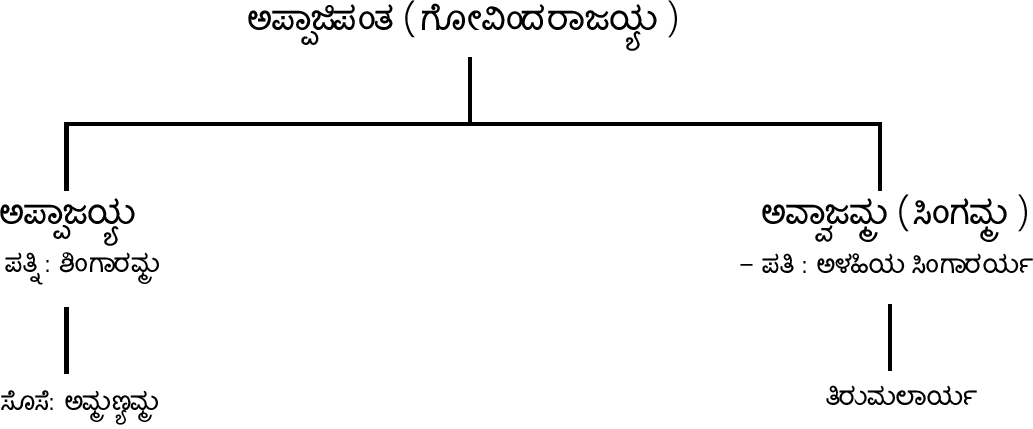
\includegraphics[scale=1.1]{"images/chap5/chap5fig1.jpeg"}
\end{figure}

ಕರಣಿಕ ಗೋವಿಂದಯ್ಯನವರ ಹೆಂಡಿರು \textbf{ಹೊನ್ನಮ್ಮನ} ಸೇವೆ ಎಂದು ಮೇಲುಕೋಟೆ ಬೆಟ್ಟದ ಮೇಲಿನ\break ಯೋಗಾನರಸಿಂಹಸ್ವಾಮಿ ದೇವಾಲಯದ ಸುತ್ತಲೂ ಇರುವ ಬಂಡೆಯ ಒಂದು ಕಡೆ ಕೆತ್ತಲಾಗಿದೆ. ಬಹುಶಃ ಇದು ಪ್ರದಕ್ಷಿಣಾಪಥವಾಗಿದ್ದು, ಈ ಬಂಡೆಯನ್ನು ಕೊರೆಯಿಸಿ, ಗೋಡೆಯನ್ನು ನಿರ್ಮಿಸುವ ಕಾರ್ಯವನ್ನು ಹೊನ್ನಮ್ಮ ಮಾಡಿಸಿರ\-ಬಹುದೆಂದು ಹೇಳಬಹುದು. ಕರಣಿಕ ಗೋವಿಂದಯ್ಯನು ಚಿಕ್ಕದೇವರಾಜನ ಮಂತ್ರಿಗಳಲ್ಲಿ ಒಬ್ಬನಾಗಿದ್ದ ಕರಣಿಕ ಲಿಂಗಣ್ಣಯ್ಯನ ಮಗನಿರಬಹುದು.


\section{ವೀರರ ಪತ್ನಿಯರು}

ವೀರರು ನಾನಾ ಕಾರಣಗಳಿಗಾಗಿ ಮಡಿದಾಗ, ಅವರಿಗಾಗಿ ವೀರಗಲ್ಲನ್ನು ಮಡಿದ ವೀರನ ತಾಯಿ, ಹೆಂಡತಿ, ಮಗಳು, ಸೋದರಿಯರು ಹಾಕಿಸುತ್ತಿದ್ದರು. ಮಡಿದ ವೀರರಿಗೆ ಬಿಟ್ಟ ದತ್ತಿಯನ್ನು ಅವರ ಕುಟುಂಬದ ಸ್ತ್ರೀಯರೇ ಪಡೆಯುತ್ತಿದ್ದರೆಂದು ಊಹಿಸಬಹುದು. ಅಧಿಕಾರವರ್ಗಕ್ಕೆ ಸೇರಿದ ವೀರರು ಮಡಿದಾಗ ಅವರ ಮನೆಯವರು ವೀರಗಲ್ಲನ್ನು ಹಾಕಿಸುತ್ತಿದ್ದರು. ಉಲ್ಲೇಖಿತ ಕೆಲವು ಶಾಸನಗಳನ್ನು ನೋಡಿದಾಗ ಇವರು ಸಾಮಾನ್ಯ ವರ್ಗಕ್ಕೆ ಸೇರಿದ ವೀರರು ಅಥವಾ ಸೈನಿಕರು ಎಂದು ಊಹಿಸಬಹುದು.

ಮಡಿವಳ್ಳ ನಾಗಿಯಣ್ಣ ತುರುಗೋಳಿನಲ್ಲಿ ಮಡಿದಾಗ, ಪುಳ್ಳಿಯಬ್ಬೆ ಮತ್ತು ಸಳಪಯ್ಯ ಕಲ್ಲನ್ನು ನೆಡಿಸಿದರೆಂದು ಮಂಚಿಬೀಡು ಶಾಸನದಲ್ಲಿ ಹೇಳಿದೆ. ಪುಳ್ಳಿಯಬ್ಬೆ ಈ ವೀರನ ತಾಯಿ ಇರಬಹುದು.\endnote{ ಎಕ 6 ಕೃಪೇ 17 ಮಂಚಿಬೀಡು 11ನೇ ಶ.} ಸುಂಕಾತೊಂಡನೂರು ಘಣ್ಟಮ್ಮನ ವೀರಗಲ್ಲಿನಲ್ಲಿ ಎರಕಬ್ಬೆಯ ಹೆಸರಿದ್ದು, ಅವಳು ಇವನ ತಾಯಿಯಾಗಿರಬಹುದು.\endnote{ ಎಕ 6 ಪಾಂಪು 243 ಸುಂಕಾತೊಂಡನೂರು 10ನೇ ಶ.} ಎರೆಯಮ್ಮನು ಬೆಗಿವಂದದ ತುರುಗೋಳಿ\-ನಲ್ಲಿ ಮಡಿದಾಗ “ಬೀಯಮ್ಮ ಕಲ್ಲನಿರಿಸಿದಳ್​” ಎಂದು ಹೇಳಿದೆ.\endnote{ ಎಕ 7 ನಾಮಂ 137 ಬೇಗಮಂಗಲ 11ನೇ ಶ.} ಬೀಯಮ್ಮ ವೀರನ ತಾಯಿಯೋ, ಅಕ್ಕ-ತಂಗಿಯೋ ಆಗಿರಬಹುದೆಂದು ಊಹಿಸಬಹುದು. ಮಂಡ್ಯ ತಾ. ಬೀಚನಹಳ್ಳಿಯ \textbf{ಒಂದನೆಯ ಬುಕ್ಕರಾಯನ ಕಾಲದ ಶಾಸನದಲ್ಲಿ, ನಲುವಶಿಯ ಭೀಮ ಎನ್ನುವವನು ಮಡಿದಾಗ ಅವನ ಸತಿ ತಿಂಮವ್ವೆಯು ವೀರಗಲ್ಲನ್ನು ನೆಡಿಸುತ್ತಾಳೆಂದು ಹೇಳಿದೆ}.\endnote{ ಎಕ 7 ಮಂ 19 ಬೀಚೇನಹಳ್ಳಿ 1341} ವಿಜಯನಗರ ಕಾಲದ ಹೊತ್ತಿಗೆ ಸಹಗಮನ ಪದ್ಧತಿ ಕಡಿಮೆ ಆಗಿತ್ತೆಂದು ಇದರಿಂದ ಊಹಿಸಬಹುದು.


\section{ಗಾವುಂಡಿಯರು}

ಗಾವುಂಡರು ವಂಶಪಾರಂಪರ್ಯವಾಗಿ ಹಳ್ಳಿಗಳ ಅಧಿಕಾರಿಗಳಾಗಿದ್ದರು. ಅವರ ಪತ್ನಿಯರನ್ನು ಶಾಸನಗಳು ಗಾವುಂಡಿಯರೆಂದು ಕರೆದಿವೆ. ಹೊಯ್ಸಳರ ಶಾಸನಗಳಲ್ಲಿ ಅನೇಕ ಗಾವುಂಡಿಯರ ಪ್ರಸ್ತಾಪ ಬಂದಿದೆ. ಇವರೂ ಕೂಡಾ ದೇವಾಲಯ, ಕೆರೆಗಳ ನಿರ್ಮಾಣ ಮತ್ತು ದತ್ತಿಗಳನ್ನು ಸ್ವತಂತ್ರವಾಗಿ ನೀಡಿರುವುದು ಕಂಡು ಬರುತ್ತದೆ. ಇವರ ಮಕ್ಕಳು ವೀರರಾಗಿದ್ದರು. ಇವರ ಗಂಡಂದಿರು ಮತ್ತು ಮಕ್ಕಳು ಇವರನ್ನು ಬಹಳ ಗೌರವದಿಂದ ನೋಡಿಕೊಳ್ಳುತ್ತಿದ್ದುದು ಶಾಸನಗಳಿಂದ ತಿಳಿದುಬರುತ್ತದೆ.

ನಾಗಮಂಗಲ ತಾಲ್ಲೂಕಿನ ಮುದಿಗೆರೆಯನ್ನು ಆಳುತ್ತಿದ್ದ ಬಾರಂದರ ಕುಲದ ಚಾಮಗಾವುಂಡನ ಮಗ ಬಿಣ್ನಾಂಡಿಯು ತನ್ನ ಮುತ್ತಬ್ಬೆ ಅಂದರೆ ಅಜ್ಜಿ (ಹೆಸರಿನ ಉಲ್ಲೇಖವಿಲ್ಲ) ಮತ್ತು ತಮ್ಮ ಅವ್ವೆ (ತಾಯಿ) \textbf{ಚಾನವ್ವೆಯರು} ಸ್ವರ್ಗಸ್ಥರಾದಾಗ ಅವರನ್ನು ಕೆರೆಯ ಮೇಲಿಕ್ಕಿ, ಅಂದರೆ ಕೆರೆಯ ಬಳಿ ಸಮಾಧಿ ಮಾಡಿ, ಅಲ್ಲಿ ಬಾರಂದೇಶ್ವರ ದೇವಾಲಯವನ್ನು ನಿರ್ಮಿಸುತ್ತಾನೆ.\endnote{ ಎಕ 7 ನಾಮಂ 98 ಮುದಿಗೆರೆ 1139} ಮಾರಗವುಡ ಹಲವರನ್ನು \textbf{ಕೊಂದು ಬಿದ್ದಾಗ ಅವನ ಮದವಳಿಗೆ ಸೋಮವ್ವೆದೇವಿಗೆ ಕೊಡಿಗೆ ಕಲ್ಲನ್ನು ಹಾಕಲಾಗಿದೆ}.\endnote{ ಎಕ 6 ಪಾಂಪು 241 ಸುಂಕಾತೊಂಡನೂರು 12ನೇ ಶ.} ಸುಂಕಾತೊಂಡನೂರಿನ 12ನೇ ಶತಮಾನದ ಈ ವೀರಗಲ್ಲನ್ನು ಗಮನಿಸಿದಾಗ ಆ ಕಾಲದಲ್ಲಿಯೇ ಸಹಗಮನವು ಕಡ್ಡಾಯ ಇರಲಿಲ್ಲ ಎಂಬುದನ್ನು ಖಚಿತವಾಗಿ ಸೂಚಿಸುತ್ತದೆ.

ಮಹಾಪ್ರಭು ಕತ್ತರಿಘಟ್ಟದ ವೃತ್ತಿಯ ಮೊಡವನಕೋಡಿಯ ಬಿಟ್ಟಿಗಾವುಡನ ಹೆಂಡತಿ \textbf{ದುಬಿಗಾವುಂಡಿಯನ್ನು}\break \textbf{“ಅರ್ಧಾಂಗ ಲಕ್ಷ್ಮಿ, ಧರ್ಮದಮೇರು, ಪಾರ್ವತಿ ಗೌರಿ, ಅಭಿಮಾನ ಸುಗ್ಗಲದೇವಿ, ಗೋತ್ರಚಿಂತಾಮಣಿ, ರಾಣಿಮೊಖಜ್ಯೋತಿ”} ಎಂದು ಶಾಸನ ವರ್ಣಿಸುತ್ತದೆ.\endnote{ ಎಕ 6 ಕೃಪೇ 111 ಮಡುವಿಅನಕೋಡಿ 1200} ಇದೇ ವಂಶದ ಮಾಚಿಗವುಡನ ಪತ್ನಿ ಮಾದಗವುಡಿಯನ್ನೂ ಮೇಲಿನ ವಿಶೇಷಣಗಳಿಂದಲೇ ಮತ್ತೊಂದು ಶಾಸನ ಹಾಡಿಹೊಗಳುತ್ತದೆ.\endnote{ ಎಕ 6 ಕೃಪೇ 100 ಮಡುವಿನಕೋಡಿ 1346}

ಮಹಾನಾಳ್ಪ್ರಭು ಬೆಳ್ಳಿಯರ ಕುಲತಿಲಕ ಧಮ್ಮಗವುಂಡನ ಪತ್ನಿ ಬೊಮ್ಮಗವುಂಡಿ. ಇವರ ಮಗ ಬಿಟ್ಟಿಗವುಂಡ. ಇವನ ಪತ್ನಿ ಬೀಚಗವುಂಡಿ. ಇವರ ಮಗ ಮಾರದೇವ. ಮಾರದೇವನ ಹೆಂಡತಿ ಮಾಚಿಗವುಡಿ. ಇವರ ಮಗ ಕಲ್ಲಗವುಡನು ಪ್ರಸಿದ್ಧನಾಗಿ ತಮ್ಮ ಅಜ್ಜ ದಮ್ಮಗವುಂಡನ ಹೆಸರಿನಲ್ಲಿ ದಮ್ಮೇಶ್ವರ ದೇವಾಲಯವನ್ನು ನಿರ್ಮಿಸುತ್ತಾನೆ.

ಶ‍್ರೀ ವೊಪ್ಪಣಾದಿ ಅಗ್ರಹಾರವಾದ ಚಿಕ್ಕಅರಸಿನಕೆರೆಯ ಮಹಾಜನಗಳು ಹಿರಿಯೀರೇಗೌಡ ಮತ್ತು ದೊಡ್ಡಿಯಮ್ಮ ಇವರುಗಳ ಮಗಳಾದ, ಮಾರವ್ವಿಗೆ ತೋಟವನ್ನು ಮಾನ್ಯವಾಗಿ ನೀಡುತ್ತಾರೆ.\endnote{ ಎಕ 7 ಮ 132 ಕ್ಯಾಗಟ್ಟ 1322} ಬೆಳಗೊಳದ ಗೌಡಿಯ ಮಗಳು \textbf{ಸಂಗಮಾಲೆ} ಎಂಬುವವಳು ಬೆಳಗೊಳದ ಕೈಲಾಸೇಶ್ವರ ದೇವಾಲಯದ ದೀಪಮಾಲೆ ಕಂಬವನ್ನು ಮಾಡಿಸಿದ್ದಾಳೆ. ಸಂಗಮಾಲೆ ಎಂಬ ಹೆಸರು ವಿಶೇಷವಾಗಿದೆ.\endnote{ ಎಕ 6 ಶ‍್ರೀಪ 72 ಬೆಳಗೊಳ} ಈಕೆ ಏನಾದರೂ ಬೌದ್ಧ ಧರ್ಮದ ಅನುಯಾಯಿಯಾಗಿದ್ದಳೆ ಎಂಬ ಊಹೆಗೆ ಅವಕಾಶವಿದೆ.


\section{ಸೆಟ್ಟಿತಿಯರು}

ವರ್ತಕ ಅಥವಾ ನಕರ ವಂಶಕ್ಕೆ ಸೇರಿದ ಸೆಟ್ಟಿಗಳ ಪತ್ನಿಯರನ್ನು ಶಾಸನಗಳಲ್ಲಿ ಸೆಟ್ಟಿತಿಯರೆಂದು ಕರೆಯಲಾಗಿದೆ. ಇವರು\break ಅನೇಕ ಧಾರ್ಮಿಕ, ಸಾಮಾಜಿಕ ಕಾರ್ಯಗಳನ್ನು ಮಾಡಿ ಶಾಸನದಲ್ಲಿ ಉಲ್ಲೇಖಿತರಾಗಿದ್ದಾರೆ. ದೋರಸಮುದ್ರದ ಪಟ್ಟಣಸ್ವಾಮಿ\-ಯಾಗಿದ್ದ ನೊಣಂಬಿಸೆಟ್ಟಿ ಅಥವಾ ಚವುಂಡಾಡಿಯ ಪತ್ನಿ ದೇಮಿಕಬ್ಬೆ ಸೆಟ್ಟಿತಿಯನ್ನು ಹೊಸಹೊಳಲು ಶಾಸನ \textbf{“ಶ‍್ರೀ ಶುಭಚಂದ್ರ ಸಿದ್ಧಾಂತ ದೇವರ ಗುಡ್ಡನಾ ಪ್ರಭುವಿನ ಮನೋನಯನವಲ್ಲಭೆ ಜಿನಗಂಧೋದಕ ಪವಿತ್ರೀಕ್ರಿತೋತ್ತಮಾಂಗೆಯರುಂ, ಆಹಾರಾಭಯ ಭೈಷಜ್ಯ ಶಾಸ್ತ್ರದಾನ ವಿನೋದೆಯರುಮಪ್ಪ ದೇಮಿಕಬ್ಬೆ ಸೆಟ್ಟಿತಿಯರು”} ಎಂದು ವರ್ಣಿಸಿದೆ.\endnote{ ಎಕ 6 ಕೃಪೇ 3 ಹೊಸಹೊಳಲು 1118} ದೇಮಾಂಬಿಕೆಯು ಕತ್ತರಿಘಟ್ಟದಲ್ಲಿ ತ್ರಿಕೂಟ ಜಿನಾಲಯವನ್ನು ಮಾಡಿಸಿ ತಮ್ಮ ಗುರು ಶುಭಚಂದ್ರ ಸಿದ್ಧಾಂತ ದೇವರಿಗೆ ದತ್ತಿಯಾಗಿ ಬಿಡುತ್ತಾಳೆ.

ಹಟ್ಟಣ ಶಾಸನವು ಪ್ರಖ್ಯಾತ ಸೋವಿಸೆಟ್ಟಿ ವಂಶದ ಮಹಿಳೆಯರ ವಿವರಗಳನ್ನು ನೀಡುತ್ತದೆ.\endnote{ ಎಕ 7 ನಾಮಂ 118 ಹಟ್ಟಣ 1199} ಈ ಶಾಸನ\-ದಲ್ಲಿ ಸ್ತ್ರೀಯರನ್ನು ಮಾಮೂಲಿ ವಿಶೇಷಣಗಳಿಂದ ವರ್ಣಿಸಲಾಗಿದೆಯೇ ಹೊರತು, ಅವರ ಸಾಧನೆಗಳೇನೆಂದು ತಿಳಿದುಬರುವುದಿಲ್ಲ. ಬಮ್ಮಿಸೆಟ್ಟಿಯ ಹೆಂಡತಿ \textbf{“ಆತ್ಮಮನೋಹರೆ ಮಾಚಿಯಕ್ಕ”.} ಇವರ ಮಗ ಗಂಧಿಸೆಟ್ಟಿಯ ಹೆಂಡತಿ \textbf{“ಅಮಲ ಶೀಲವತಿ ಮಾಸತಿ ಕಾಂತೆ ಲಕ್ಷ್ಮಿವೋಲ್​ ಎಸೆವೆ ಮಾಕವ್ವೆ”,} ಇವರ ಮಗ ಸೋವಿಸೆಟ್ಟಿಯ ಹೆಂಡತಿ \textbf{“ಪರಮ ಜಿನಪದಕಮಳೆ ಮಧುಕರಿ, ದಾನವಿನೋದೆ, ಗೋತ್ರಚಿಂತಾಮಣಿ, ಬಂಧುರಿಮಗುಣಿ, ಸುಶೀಲೆ ಪುಣ್ಯವತಿ ಮರುದೇವಿ”.} ಸೋವಿಸೆಟ್ಟಿಯು ಪಟ್ಟಣದಲ್ಲಿ ತಟಾಕತ್ರಯವನ್ನು, ಉತ್ತುಂಗ ಚೈತ್ಯಾಲಯವನ್ನು ಕಟ್ಟಿಸುತ್ತಾನೆ. ಮಂಡಲಸ್ವಾಮಿ ಕೇತಿಸೆಟ್ಟಿಯ ವಂಶದ ಮಹಿಳೆಯರ ಉಲ್ಲೇಖ ಬೆಳ್ಳೂರಿನ ಶಾನಸದಲ್ಲಿ ಬಂದಿದೆ. ಬಾವಿಸೆಟ್ಟಿಯ ಹೆಂಡತಿ \textbf{ಸೂಚಿಕಬ್ಬೆ}. ಇವರ ಮಗ ಬೆಳ್ಳೂರಿನ ಮಂಡಲಸ್ವಾಮಿಯಾಗಿದ್ದ ಕೇತಿಸೆಟ್ಟಿ. ಕೇತಿಸೆಟ್ಟಿಯ ಹೆಂಡತಿ \textbf{“ವನಿತಾತಿಳಕ ಸಮಾನೆ ಮಾಚವ್ವೆ”.} ಈ ಮಂಡಲಸ್ವಾಮಿಯು ಬೆಳ್ಳೂರಿನಲ್ಲಿ ಮಂಡಲೇಶ್ವರ ದೇವಾಲಯವನ್ನು ನಿರ್ಮಿಸುತ್ತಾನೆ.\endnote{ ಎಕ 7 ನಾಮಂ 80 ಬೆಳ್ಳೂರು 1199} ಪತಿಯ ಧರ್ಮಕಾರ್ಯಗಳಲ್ಲಿ ಪತ್ನಿಯರೂ ಸಹಕರಿಸುತ್ತಿದ್ದರೆಂದು ಊಹಿಸಬಹುದು.


\section{ಅಧಿಕಾರಿಗಳ ಪತ್ನಿಯರು}

ಆಡಳಿತ ವ್ಯವಸ್ಥೆಯಲ್ಲಿ ವಿವಿಧ ಮಟ್ಟದ ಅಧಿಕಾರಗಳನ್ನು ಹೊಂದಿದ್ದ ಅಧಿಕಾರಿಗಳ ಪತ್ನಿಯರು ಹಾಗೂ ಅವರ ಸಾಧನೆಗಳ ಉಲ್ಲೇಖ ಜಿಲ್ಲೆಯ ಶಾಸನಗಳಲ್ಲಿ ತಕ್ಕಮಟ್ಟಿಗೆ ಉಲ್ಲೇಖಗೊಂಡಿದೆ. ಮಹಾಪಸಾಯಿತ ಪಟ್ಟಸಾಹಣಿ ಅರಸಿಯಕರೆಯ ಮಹದೇವಣ್ಣನ ಪತ್ನಿ \textbf{ನನ್ನವ್ವೆಯ} ವರ್ಣನೆ ಕಸಲಗೆರೆ ಶಾಸನದಲ್ಲಿ ಬಂದಿದೆ.\endnote{ ಎಕ 7 ನಾಮಂ 168 ಕಸಲಗೆರೆ 1190}

ಪೆರ್ಗ್ಗಡೆ ಮಲ್ಲಿಯಣ್ಣನ ತಾಯಿ \textbf{ಮಾರವ್ವೆ.}\endnote{ ಎಕ 7 ಮ 29 ಆಬಲವಾಡಿ 1131} ಈ ಶಾಸನದಲ್ಲಿ ಮಲ್ಲಿನಾಥನ ವಿವರಗಳ ನಂತರ ಈಕೆಯ ವಿವರವೂ ಬಂದಿರುವುದರಿಂದ ಈಕೆ ಇವನ ಪತ್ನಿಯಾಗಿರಬಹುದೆಂದು ಹ.ಕ. ರಾಜೇಗೌಡರು ಹೇಳುತ್ತಾರೆ.\endnote{ ರಾಜೇಗೌಡ ಹ.ಕ., ಮಂಡ್ಯ ಜಿಲ್ಲೆಯ ಶಾಸನಗಳಲ್ಲಿ ಸ್ತ್ರೀಯರು, ಸಿರಿಯೊಡಲು, ಪುಟ} ಆದರೆ ಶಾಸನ ತ್ರುಟಿತವಾಗಿದ್ದು, ಮೊದಲು ವಿಷ್ಣುವರ್ಧನನ ಉಲ್ಲೇಖದ ನಂತರ ಮಲ್ಲಿನಾಥನನ್ನು ಉಲ್ಲೇಖಿಸಿ, ಅವನ ವಂಶವೃಕ್ಷವನ್ನು ವರ್ಣಿಸುವಾಗ ಮಾಚಿಕೆಯ ಹೆಸರು ಉಲ್ಲೇಖವಾಗಿದೆ. ಆದಕಾರಣ \textbf{ಮಾಚಿಕೆಯು} ಮಲ್ಲಿನಾಥನ ತಾಯಿ ಆಗಿರಬಹುದು. ಮಲ್ಲಿನಾಥನ ಉಲ್ಲೇಖವಿರುವ ಶ್ರವಣಬೆಳಗೊಳ ಶಾಸನದಲ್ಲೂ ವಿವರಗಳು ಸಿಗುವುದಿಲ್ಲ.\endnote{ ಎಕ 2 ಶ್ರವಣಬೆಳಗೊಳ 81 ಚಿಕ್ಕಬೆಟ್ಟ 12ನೇ ಶ.}

ಹಡವಳರ(ಪಡೆವಳ) ಪತ್ನಿಯರ ಉಲ್ಲೇಖ ಕೆಲವು ಶಾಸನಗಳಲ್ಲಿ ಬಂದಿದೆ. ಹಡವಳದ ಕೊಳ್ಳಿಮಯ್ಯನ \textbf{“ಸರ್ಭಾಂಗ ಲಕ್ಷುಮಿ ಚಾಮುಂಡವ್ವೆ”.\endnote{ ಎಕ 6 ಕೃಪೇ 42 ತೆಂಗಿನಘಟ್ಟ 1117}} ಕುಂನಿಯ ಕೋಲ ಹಡವಳ ಹೊನ್ನಯ್ಯನ \textbf{“ಭಾರ್ಯೆ ಸಿವಪಾದಸೇಖರೆ ಶಿವಕಥಾಳಾಪೆ ಶಿವಪಾದೋದಕೆ ದೇಗುಲಗೌಣ್ಡಿ”.}\endnote{ ಎಕ 7 ನಾಮಂ 107ಹೊನ್ನೇನಹಳ್ಳಿ 1180} ದೇಗುಲಗೌಂಡಿಯ ಶಿವಭಕ್ತಿಯ ವರ್ಣನೆಯನ್ನು ನೋಡಿದರೆ ಈಕೆ ಶೈವಧರ್ಮಕ್ಕೆ ಅಪಾರ ಸೇವೆ ಸಲ್ಲಿಸಿರಬಹುದೆಂದು ತೋರುತ್ತದೆ. ಹಡವಳಿತಿಯರು ಭೂಮಿಯನ್ನು ಹೊಂದಿರುತ್ತಿದ್ದರು. ಕೆರೆಗಳನ್ನು ಕಟ್ಟಿಸುತ್ತಿದ್ದರು. \textbf{“ಹಡವಳಿತಿಯ ಹೊಲ, ಹಡವಳಿತಿಯ ಹೊಲದೊಳಗೆ ಸಲ್ಲುವ ಹಿರಿಯ ಕೆರೆ, ಹಡವಳಿತಿಯ ಬೆದ್ದಲೆ, ಹಡವಳಿತಿಯ ಕೆರೆಯ ಪಡುವಣ ಕೋಡಿ”} ಎಂಬ ಉಲ್ಲೇಖಗಳು ಅಳೀಸಂದ್ರ ಶಾಸನದಲ್ಲಿ ಬಂದಿರುವುದನ್ನು ಗಮನಿಸಬಹುದು. ಕರದಾಳದ ಮಲ್ಲಿದೇವನ ಹೆಂಡತಿ ಚನ್ನದೇವಿಯು ಹೊಲತ್ತಿ(ಹಾಲತಿ)ಯಲ್ಲಿದ್ದ ತನ್ನ ಕೊಡಗಿಯ ಹೊಲವನ್ನು ದೇವರಿಗೆ ದತ್ತಿಯಾಗಿ ಬಿಡುತ್ತಾಳೆ.


\section{ಸಾಮಾನ್ಯ ಸ್ತ್ರೀಯರು}

ಯಾವುದೇ ಅಧಿಕಾರ ಸ್ಥಾನದಲ್ಲಿ ಇಲ್ಲದಿರುವ ಸಾಮಾನ್ಯ ಸ್ತ್ರೀಯರೂ ಕೂಡಾ ಶಾಸನಗಳಲ್ಲಿ ಸ್ಥಾನ ಪಡೆದಿದ್ದಾರೆ. ಮಹಿಳೆಯರು ಶಾಸನದಲ್ಲಿ ಸ್ಥಾನ ಪಡೆಯುವುದು ಕಷ್ಟವಿತ್ತು ಎಂಬುದನ್ನು ಅಳಿಸಂದ್ರ ಶಾಸನದ ಪದ್ಯವೊಂದು ಇತರ ಮಹಿಳೆಯರು ಲೋಕದ ಗಣಿಕೆಯರಿದ್ದಂತೆ, ಶಾಸನದಲ್ಲಿ ಸ್ಥಾನಪಡೆಯುವವಳು ಶಾಸನದೇವಿಯರಿದ್ದಂತೆ ಎಂದು ಹೇಳಿದೆ.\endnote{ ಎಕ 7 ನಾಮಂ 72 ಅಳೀಸಂದ್ರ 1183}

\textbf{ಜೈನಧರ್ಮದ ಮಹಿಳೆಯರು: } ಜೈನಧರ್ಮದಲ್ಲಿ ಸಾಮಾನ್ಯ ಸ್ತ್ರೀಯರೂ ಗೌರವಾದರಗಳಿಗೆ ಪಾತ್ರರಾಗಿದ್ದರು. ಅವರು ತಮ್ಮ ಜೀವಿತದ ಅಂತ್ಯ ಕಾಲದಲ್ಲಿ ಅಥವಾ ತಮ್ಮ ಬಾಳು ಸಾಕೆನೆಸಿದಾಗ, ಜೈನಧರ್ಮದ ನಿಯಮಗಳ ಪ್ರಕಾರ ಸನ್ಯಸನ ವಿಧಿಯಿಂದ ದೇಹತ್ಯಾಗ ಮಾಡುತ್ತಿದ್ದುದು ತಿಳಿದೇ ಇದೆ. ಕೆಲವರು ಕಂತಿಯರಾಗಿ ಈ ನಿಯಮ ಅನುಸರಿಸಿ ಮೃತರಾದರೆ, ಇನ್ನು ಕೆಲವು ಗೃಹಸ್ಥೆಯರು ಅಥವಾ ಶ್ರಾವಿಕೆಯರು ಉಪವಾಸ ವ್ರತದಿಂದ ದೇಹತ್ಯಾಗ ಮಾಡುತ್ತಿದ್ದರು. ತಮ್ಮ ಪ್ರೀತಿಪಾತ್ರರು ಈ ವಿಧಿಯಿಂದ ಮರಣ ಹೊಂದಿದಾಗ ಸ್ತ್ರೀಯರೇ ನಿಸಿದಿಗೆಯನ್ನು ನಿರ್ಮಿಸುತ್ತಿದ್ದ ಉದಾಹರಣೆಗಳು ಕಂಡುಬರುತ್ತವೆ.

ಪ್ರಭಾಚಂದ್ರ ಸೈದ್ಧಾಂತಿಕರು ತಮ್ಮ ಶಿಷ್ಯಿತಿಯರಾದ \textbf{“ರುಕಮವ್ವೆ ಜಕ್ಕವ್ವೆ ಕನ್ತಿಯರ್ಗೆ ನಿಸಿದಿಯಂ ಮಾಡಿಸಿ\general{\break }ಸ್ವರ್ಗಸ್ಥರಾದರು” ಎಂದು ಹೇಳಿದ್ದು, ಇವರ ಮರಣದ ನಂತರ ಇವರಿಗೆ ನಿಸಿದಿಗೆಯನ್ನು ಮಾಡಿಸಿ ಗುರುವೂ ಮರಣಹೊಂದಿದ್ದಾನೆ. ಮೂವರೂ ಒಟ್ಟಿಗೆ ಸಲ್ಲೇಖನ ವ್ರತವನ್ನು ಅನುಸರಿಸುತ್ತಿದ್ದರೆಂದು ಹೇಳಬಹುದು.}\endnote{ ಎಕ 7 ನಾಮಂ 28 ಕಂಬದಹಳ್ಳಿ 12ನೇ ಶ.} ಶ್ರವಣಬೆಳಗೊಳದ ಶಾಸನದಲ್ಲಿ ಜಕ್ಕವ್ವೆ ಮೈದುನ ಬೊದ್ದಿಸೆಟ್ಟಿ ಎಂಬ ಉಲ್ಲೇಖವಿದೆ. ಬಹುಶಃ ಈ ಜಕ್ಕವ್ವೆ ಕಂಬದಳ್ಳಿ ಶಾಸನೋಕ್ತ ಜಕ್ಕವ್ವೆಯೇ ಆಗಿದ್ದಾಳೆಂದು ಹೇಳಬಹುದು.\endnote{ ಎಕ 2 ಶ್ರಬೆ 356 ದೊಡ್ಡಬೆಟ್ಟ 12ನೇ ಶ.}

ತಂದೆಯು ಸನ್ಯಸನ ವಿಧಿಯಿಂದ ಮರಣ ಹೊಂದಿದಾಗ ಅವನ ಮಗಳಾದ \textbf{ಬಿಡಕ್ಕ} ನಿಸಿದಿಗೆಯನ್ನು ಮಾಡಿಸುತ್ತಾಳೆ.\endnote{ ಎಕ 7 ನಾಮಂ 24 ಕೋಡಿಹಳ್ಳಿ 10ನೇ ಶ.} ಉಭಯಭಾಷಾ ಕವಿಚಕ್ರವರ್ತಿ ಕಂದರ್ಪದೇವರ ಮದುವಳಿಗೆ \textbf{ಸೊನ್ನಾದೇವಿಯ} ಉಲ್ಲೇಖ ತಿಪ್ಪೂರು ಶಾಸನದಲ್ಲಿದೆ. ಇವಳ ಮಗ ಕಾಣೂರ್ಗ್ಗಣ ತಿಳಕನುಮಪ್ಪ ಬಾಳಚಂದ್ರದೇವ ಎಂದು ತಿಳಿದುಬರುತ್ತದೆ.\endnote{ ಎಕ 7 ಮ 54 ತಿಪ್ಪೂರು 1117} ತಮ್ಮ ಗುರುಗಳು ಮುಡಿಪಿದಾಗ ಅವರ ಶಿಷ್ಯೆ \textbf{ಮಾದೇವಿ ಕಂತಿಯರು} ನಿಸಿದಿಗೆಯ ಕಂಬವನ್ನು ಇರಿಸಿದರು ಎಂದು ಮಾರಗಾನಹಳ್ಳಿ ಗೋಗಲ್ಲು ಶಾಸನದಲ್ಲಿದೆ.\endnote{ ಎಕ 7 ಮ 143 ಮಾರಗಾನಹಳ್ಳಿ 13ನೇ ಶ.} ಈ ಶಾಸನದಲ್ಲಿ ಶ‍್ರೀಮತ್​ \textbf{ಬಾವಿತ್ತೆಯದಕ್ಕ} ಎಂಬ ಉಲ್ಲೇಖವಿದ್ದು ಈಕೆಯೂ ಕಂತಿಯಾಗಿರಬಹುದೆಂದು ಊಹಿಸಬಹುದು.

\textbf{ಶೈವಧರ್ಮದ ಮಹಿಳೆಯರು: } ಶೈವಧರ್ಮದ ಸ್ಥಾನಪತಿಗಳ ಮನೆತನದ ಸ್ತ್ರೀಯರೂ ಶಾಸನೋಕ್ತರಾಗಿದ್ದಾರೆ. ಧರ್ಮರಾಸಿ ಪಂಡಿತರ \textbf{ಮದವಳಿಗೆ ಹೊನ್ನವ್ವೆಗೆ} ಮತ್ತು ಆಕೆಯ ಇಬ್ಬರು ಮಕ್ಕಳಿಗೆ ಬಮ್ಮಣ್ಣನವೆಂಬುವವನು ಭಟಾರ ದೇವಾಲಯನ್ನು ಕಟ್ಟಿಸಿದಾಗ ದತ್ತಿಯನ್ನು ಬಿಡುತ್ತಾನೆ.\endnote{ ಎಕ 6 ಪಾಂಪು 252 ತಿರುಮಲಸಾಗರ ಛತ್ರ 1125} ಶಾಸನ ಕವಿ ಸಾಂತಮಹಂತನು ತನ್ನ ತಾಯಿ ಸೋಮಿಯಕ್ಕನನ್ನು \textbf{“ಕ್ಷಿತಿವಿನುತೆ ಸರ್ಬ್ಬದೇವನುತೆ ಸಂನುತೆ ಸೋಮಿಯಕ್ಕನಣುಗಿನ ಪುತ್ತ್ರಂ ಸತುಕವಿ ಸಾಂತಮಹಂತಂ”} ಎಂದು ಪ್ರೀತಿಗೌರವಗಳಿಂದ ವರ್ಣಿಸಿದ್ದಾನೆ.\endnote{ ಎಕ 7 ನಾಮಂ 61 ಲಾಳನಕೆರೆ 1138}ಸೋಮೇಶ್ವರ ಪಂಡಿತರ ಸ್ತ್ರೀ (ಪತ್ನಿ) \textbf{ಚಾಮವ್ವೆಯು} ಆರಣಿಯ ಕೆರೆಯ ಏರಿಯ ಮೇಲೆ ಚಾಮುಂಡೇಶ್ವರಿ ದೇವಿಯ ವಿಗ್ರಹವನ್ನು ಪ್ರತಿಷ್ಠಾಪಿಸಿದ್ದಾಳೆ.\endnote{ ಎಕ 7 ನಾಮಂ 101 ಆರಣಿ. 13 ನೇ ಶ.}ಸಿಂಗಳದೇವ ಒಡೆಯರ ಶಿಷ್ಯೆ (ಸಿಸ್ಯಿ) \textbf{ಚಿಕ್ಕಿಯರ} ಮಗ ಮುದ್ದಣ್ಣನ ಪ್ರಸ್ತಾಪ ಪ್ರಾಚೀನ ಶೈವಕೇಂದ್ರವಾದ ಹಾಲತಿಯ ಶಾಸನದಲ್ಲಿ ಬರುತ್ತದೆ.\endnote{ ಎಕ7 ನಾಮಂ 139 ಹಾಲ್ತಿ 1605}

\textbf{ವೈಷ್ಣವಧರ್ಮದ ಮಹಿಳೆಯರು:} ವೈಷ್ಣವಧರ್ಮದ ಅನುಯಾಯಿಗಳಾದ ಸಾಮಾನ್ಯ ಸ್ತ್ರೀಯರ ಉಲ್ಲೇಖ ಶಾಸನಗಳಲ್ಲಿ ಹೆಚ್ಚಾಗಿ ಕಂಡುಬರುತ್ತದೆ. ಈ ಧರ್ಮದಲ್ಲಿ ಸ್ತ್ರೀಯರಿಗೆ ಹೆಚ್ಚಿನ ಸ್ವಾತಂತ್ರ್ಯವೂ ಮಾನ್ಯತೆಯೂ ಇರುವುದು ಈ ಶಾಸನಗಳ ಅಧ್ಯಯನದಿಂದ ಕಂಡುಬರುತ್ತದೆ. ಕೆಲವು ಸಲ ಇವರ ಪತಿಯರ, ತಂದೆ ತಾಯಿಗಳ ಹೆಸರು ಶಾಸನಗಳಲ್ಲಿ ಕಾಣಿಸಿಕೊಂಡರೂ, ಅವರು ಯಾವ ಅಧಿಕಾರ ಸ್ಥಾನದಲ್ಲಿದ್ದರೆಂಬುದು ತಿಳಿದುಬರುವುದಿಲ್ಲ.

ಮಟ್ಟಿಯಮ್ಬಾಕ್ಕಮ್ ಗ್ರಾಮದ ಇಳೈಯಭಿರಾನ್​ಭಟ್ಟನ ಪತ್ನಿ ನಂಗೈ ಆಂಡಾಳ್​ ಯಾದವನಾರಾಯಣ ಚತುರ್ವೇದಿ ಮಂಗಲದ ಅಂದರೆ, ತೊಂಡನೂರಿನಲ್ಲಿ ಚೊಕ್ಕಾಣ್ಡೈ ಪೆರ್ಗಡೆ ಎಂಬುವವನು ಬೆಟ್ಟದಮೇಲೆ ಕಟ್ಟಿಸಿದ್ದ ಮಲೈಮೇಲ್​\break ಸಿಂಗಪೆರುಮಾಳ್​ ಅಥವಾ ನರಸಿಂಹದೇವರ ಆಲಯದಲ್ಲಿ ವೆಣ್ಣೈಕೂತ್ತಪಿಳ್ಳೆ ಅಂದರೆ ಕೃಷ್ಣನ ಪ್ರತಿಮೆಯನ್ನು ಪ್ರತಿಷ್ಠಾಪಿಸಿ ಅದರ ಸೇವೆಗಾಗಿ ಹತ್ತು ಹೊನ್ನನ್ನೂ,\endnote{ ಎಕ 6 ಪಾಂಪು 120 ತೊಣ್ಣೂರು 1136} ಮತ್ತೆ ತಾನು ಪ್ರತಿಷ್ಠಾಪಿಸಿದ ಈ ಪಿಳ್ಳೈದೇವರ ಜಯಂತಿ ಉತ್ಸವ ಹಾಗೂ ಮೆರವಣಿಗೆಗೆ ಮತ್ತೆ ಆರು ಹೊನ್ನುಗಳನ್ನು ದತ್ತಿಯಾಗಿ ಬಿಡುತ್ತಾಳೆ.\endnote{ ಎಕ 6 ಪಾಂಪು 119 ತೊಣ್ಣೂರು 1152} ಪಟ್ಟದ ಅಗ್ರಹಾರ ಸರ್ವಜ್ಞವೀರನರಸಿಂಹಪುರವಾದ ಅರಕೆರೆಯಲ್ಲಿದ್ದ ಪ್ರಭಾಕರದ ವಿದ್ವಾಂಸ ಕುಮಾಂಡೂರಾಚರ ಹೆಂಡತಿ \textbf{ಅಯ್ಯಾದಕ್ಕ}, ತನಗೆ ಸೇರಿದ ವೃತ್ತಿಯಲ್ಲಿ, ಪಾದ ವೃತ್ತಿಯನ್ನು (ಕಾಲುಭಾಗ) \textbf{ಸ್ತ್ರೀ, ಪುತ್ರ, ಜ್ಞಾತಿ, ಸ್ವಗ್ರಾಮಿ, ಸಾಮಂತ, ದಾಯಾದಿ ಇವರ ಅನುಮತಿಯ ಪ್ರಕಾರ} ಚನ್ನಕೇಶವ ದೇವರಿಗೆ ದತ್ತಿ ಬಿಡುತ್ತಾಳೆ. ಈ ದತ್ತಿಗೆ ಸೇರಿದ ಭೂಮಿಯಲ್ಲಿ ಬರುವ ಬೆಳೆ ಹಾಗೂ ಉತ್ಪತ್ತಿಯನ್ನು ಆ ದೇವರ “ತಿರಿನಂದನವನ”ವನ್ನು ನಿರ್ವಹಣೆ ಮಾಡುವವರು, ಪ್ರತಿವರ್ಷ ತಮ್ಮ ಜೀವಿತ ಮುಖ್ಯವಾಗಿ, ಆ ದೇವರ ಶ‍್ರೀಕಾರ್ಯ, ಅಂಗಭೋಗಕ್ಕೆ ಕೊಡುವಂತೆ ಕಟ್ಟುಪಾಡನ್ನು ವಿಧಿಸುತ್ತಾಳೆ.\endnote{ ಎಕ 6 ಶ‍್ರೀಪ 98 ಅರಕೆರೆ 1254} ಶ‍್ರೀವೈಷ್ಣವ ಧರ್ಮಕ್ಕೆ ಸೇರಿದ ಮಹಿಳೆಯಾದ ಈಕೆಯು ತನ್ನ ವೃತ್ತಿಯನ್ನು ದೇವರಿಗೆ ದತ್ತಿ ಬಿಡುವಾಗ ಎಲ್ಲರ ಒಪ್ಪಿಗೆಯನ್ನು ಪಡೆಯುತ್ತಾಳೆ. ಸ್ತ್ರೀಯರು ತಮಗೆ ಸೇರಿದ ವೃತ್ತಿಯನ್ನು ದಾನ ಮಾಡುವಾಗ ಸಂಬಂಧಿಸಿದವರ ಒಪ್ಪಿಗೆ ಪಡೆಯಬೇಕಾಗುತ್ತಿತ್ತು ಎಂಬುದು ಇದರಿಂದ ತಿಳಿದುಬರುತ್ತದೆ. ತೊಣ್ಣೈಕೂಡು ಶ‍್ರೀವುರಮಂಗಲದ ಅಂದರೆ ಇಂದಿನ ಶ‍್ರೀರಂಗಪಟ್ಟಣದ ತಿರುವರಂಗ ಮುಡೈಯಾನವನ್​ನ ಧರ್ಮಪತ್ನಿ \textbf{ಕಲ್ಪಗಂಕೊಂಡಾಳ್​}. ಇವರ ಮಗ ವರಂತರುಮ್ ಪೆರುಮಾನ್​. ಈತನು ಮಹಾಜನರಿಗೆ ದತ್ತಿ ಬಿಡುತ್ತಾನೆ.\endnote{ ಎಕ 6 ಶ‍್ರೀಪ 1 ಶ‍್ರೀರಂಗಪಟ್ಟಣ 1210} ಯಾದವ ನಾರಾಯಣ ಚತುರ್ವೇದಿ ಮಂಗಲವಾದ ತೊಂಡನೂರಿನ ನಡುವಣ ದೇವಾಲಯದ ವೀರ್ರಿರುಂದ ಪೆರುಮಾಳೈ ದೇವರ ನಂದಾದೀಪಕ್ಕೆ ಅದೇ ಊರಿನ \textbf{ಕೋದೈಯಾಣ್ಡಾಳಮ್ಮೈ} ಅರ್ಧವೃತ್ತಿಯನ್ನು ದತ್ತಿಯಾಗಿ ಬಿಡುತ್ತಾಳೆ.\endnote{ ಎಕ 6 ಪಾಂಪು 82 ತೊಣ್ಣೂರು 13ನೇ ಶ.} ಇದೇ ದೇವರಿಗೆ ಕುಚಪ್ಪವಿಲ್​ ಸೀತೈಯಾಣ್ಡಾಳ್​ ನಂಗೈಯಾರ್​ ತಿರುವರಾಧಾನೆಗೆ ಒಂದು ವೃತ್ತಿಯನ್ನು ಬಿಡುತ್ತಾಳೆ.\endnote{ ಎಕ 6 ಪಾಂಪು 84 ತೊಣ್ಣೂರು 13ನೇ ಶ.} ಕೌಶಿಕಗೋತ್ರದ \textbf{ಪುಂಗನೂರ ಚನ್ನಮ್ಮ} ಶ‍್ರೀಮಾಧವ ಪೆರುಮಾಳ ತಿರುನಂದಾದೀಪಕ್ಕೆ ಮೂರು ಹೊನ್ನನ್ನು ಇಟ್ಟು ಅದರ ಬಡ್ಡಿಯನ್ನು ದತ್ತಿಯಾಗಿ ಬಿಡುತ್ತಾಳೆ\endnote{ ಎಕ 7 ಮ 126 ದೊಡ್ಡಅರಸಿನಕೆರೆ 13-14ನೇ ಶ.} ತುಗವಿ ಮಂಡೂರಿನ ಪೆರಿಯಪೆರುಮಾಳ್​ನ ಹೆಂಡತಿ \textbf{ಬ್ರಾಹ್ಮಣಿ ಅಲ್ಲಾಳಿ} ಮಾರೆಹಳ್ಳಿ ಲಕ್ಷ್ಮೀನರಸಿಂಹ ದೇವಾಲಯದ ಮುಖಮಂಟಪದ ನಿರ್ಮಾಣಕ್ಕೆ, ಇಪ್ಪತ್ತು ಪಣವನ್ನು ದತ್ತಿಯಾಗಿ ಬಿಡುತ್ತಾಳೆ.\endnote{ ಎಕ 7 ಮವ 68 ಮಾರೆಹಳ್ಳಿ 13ನೇ ಶ.} ಮಾರೆಹಳ್ಳಿಯ ಲಕ್ಷ್ಮೀನರಸಿಂಹ ದೇವರಿಗೆ \textbf{ಕುಪ್ಪಮ್ಮನು} ಹಿತ್ತಾಳೆಯ ಮಾವಿನ ಎಲೆಯ ತೋರಣವನ್ನು ಮಾಡಿಸಿಕೊಡುತ್ತಾಳೆ.\endnote{ ಎಕ 7 ಮವ 66 ಮಾರೆಹಳ್ಳಿ 19ನೇ ಶ.}

ಮೇಲುಕೋಟೆಯ ನಾರಾಯಣ ದೇವಾಲಯದಲ್ಲಿರುವ ಬೆಳ್ಳಿಯ ಕೊಡವನ್ನು, ರಾಮಾಯಣದ\break ತಿರುಮಲಾಚಾರ್ಯರ ಧರ್ಮಪತ್ನಿಯರಾದ \textbf{ನಾಚಾರಮ್ಮ} ಮತ್ತು \textbf{ತಿರುವೆಂಗಡಮ್ಮ} ಮಾಡಿಸಿಕೊಟ್ಟಿದ್ದಾರೆ.\endnote{ ಎಕ 6 ಪಾಂಪು 173 ಮೇಲುಕೋಟೆ, ಸು. 1725} ಇದೇ\break ನಾರಾಯಣಸ್ವಾಮಿ ದೇವಾಲಯದಲ್ಲಿರುವ ಬೆಳ್ಳಿಯ ಪುಷ್ಪತಟ್ಟೆಯನ್ನು, ಮೇಲುಕೋಟೆ \textbf{ಕಲ್ಯಾಣಿ ಕೆಂಪಮ್ಮನ} ಮಗಳು\break \textbf{ಪುಟ್ಟಶಿಂಗಮ್ಮನು} ಮಾಡಿಸಿಕೊಟ್ಟಿದ್ದಾಳೆ.\endnote{ ಎಕ 6 ಪಾಂಪು 174 ಮೇಲುಕೋಟೆ 18ನೇ ಶ.} ಈ ದೇವಾಲಯದಲ್ಲಿರುವ ಬೆಳ್ಳಿಬಟ್ಟಲನ್ನು ಮೇಲುಕೋಟೆಯ \textbf{ಪುಟ್ಟನರಸಮ್ಮನು} ನರಸಿಂಹದೇವರಿಗೆ ಮಾಡಿಸಿಕೊಟ್ಟಿದ್ದಾಳೆ.\endnote{ ಎಕ 6 ಪಾಂಪು 175 ಮೇಲುಕೋಟೆ 18 ನೇ ಶ.} ಈಗಲೂ ಇದನ್ನು \textbf{ಪುಟ್ಟನರಸಿ ಬೆಳ್ಳಿಬಟ್ಟಲು} ಎಂದೇ ಈಗಲೂ ಕರೆಯಲಾಗುತ್ತಿದೆ.

ಶ‍್ರೀರಂಗಪಟ್ಟಣದ ಬಳಿ ಇರುವ ಶ‍್ರೀನಿವಾಸ ಕ್ಷೇತ್ರವೂ ಕೂಡಾ ಒಂದು ವೈಷ್ಣವಕೇಂದ್ರವಾಗಿತ್ತು. ಶ‍್ರೀನಿವಾಸಕ್ಷೇತ್ರದ ನರಸಿಂಹಶಠಕೋಪ ಸ್ವಾಮಿಯವರ ಸನ್ನಿಧಿಯಲ್ಲಿ, ನಿರವಧಿಕ ನಿತ್ಯ ತದೀಯಾರಾಧನವು ನಡೆಯಲು ಹರಿತ್ಸ ಗೋತ್ರದ ರಾಮೈಯಂಗಾರರ ಪುತ್ರಿ \textbf{ನಾಚಾರಮ್ಮನು} ಎಂಟು ಅಂಕಣ ಶಿಲಾದ (ಶಿಲೆಯಿಂದ ನಿರ್ಮಿತವಾದ) ಶ‍್ರೀಮಠವನ್ನು ಮಾಡಿಸಿ ಸಮರ್ಪಿಸುತ್ತಾಳೆ.\endnote{ ಎಕ 6 ಶ‍್ರೀಪ 82 ಶ‍್ರೀನಿವಾಸಕ್ಷೇತ್ರ 1847} ಶ‍್ರೀನಿವಾಸ ಕ್ಷೇತ್ರದ ಬಳಿ ಕಾವೇರಿ ಹೊಳೆಗೆ ಇಳಿಯುವ ಸೋಪಾನವನ್ನು \textbf{ವಾರಣಾಸಿಯ ನಂಜಮ್ಮ} ಮಾಡಿಸಿದ್ದಾಳೆ.\endnote{ ಎಕ 6 ಶ‍್ರೀಪ 83 ಶ‍್ರೀನಿವಾಸಕ್ಷೇತ್ರ 19ನೇ ಶ.} ಆಳಿದ ಮಹಾಸ್ವಾಮಿಯವರ ಪಾದಸೇವಕಳಾದ \textbf{ಸಂಬಂಮನ} (ಸಾಂಬಮ್ಮ) ತಾಯಿ \textbf{ದೊಡ್ಡನಂಜಮ್ಮನ} ಮಗಳು \textbf{ಹೊಸೂರು ವೆಂಕಟಲಕ್ಷ್ಮಮ್ಮನು} ಮದ್ದೂರು ನರಸಿಂಹಸ್ವಾಮಿಗೆ ಬೆಳ್ಳಿಮುಲಾಮಿನ ದೊಡ್ಡ ಗರುಡವಾಹನವನ್ನು ಮಾಡಿಸಿಕೊಡುತ್ತಾಳೆ.\endnote{ ಎಕ 7 ಮ 13 ಮದ್ದೂರು 1851}\textbf{ “ಬೆಳಗೊಳದ ವಳಾಯ ಮಳಗಿಯರ ವೊಡವುಟ್ಟಿದ ಅಕಬೆಯುಂ(ಅಕ್ಕಬ್ಬೆ) ಪೆರುಂದೇವಿಯುಂ\general{\break } ನಾರಾಯಣದೇವರ ತ್ತಿರ್ಮಾಲೆಗೆ”} ಅಂದರೆ ತಿರುಮಾಲೆಗೆ ಗದ್ದೆಯನ್ನು ದಾನವಾಗಿ ನೀಡಿ, ಅದನ್ನು ತಿರಿಕಂಣ್ನದರ ಜೀಯರು ನಡೆಸಿಕೊಂಡು ಹೋಗುವಂತೆ ಹೇಳಿದ್ದಾರೆ.\endnote{ ಎಕ 6 ಪಾಂಪು 178 ಮೇಲುಕೋಟೆ 18ನೇ ಶ.} ಅಕಬ್ಬೆ ಮತ್ತು ಪೆರುಂದೇವಿ ಎಂಬ ಹೆಸರುಗಳು ಜೈನಧರ್ಮದ ಮಹಿಳೆಯರ ಹೆಸರಿನಂತೆ ಕಂಡುಬರುತ್ತವೆ. ಜೊತೆಗೆ ಈ ಮಹಿಳೆಯರು ಬೆಳಗೊಳದವರಾಗಿದ್ದಾರೆ. ಜೈನಧರ್ಮದ ಮಹಿಳೆಯರೂ ಕೂಡಾ ವೈಷ್ಣವ ದೇವರಿಗೆ ದತ್ತಿ ಬಿಟ್ಟಿರುವುದು ಗಮನಾರ್ಹವಾದ ವಿಚಾರವಾಗಿದೆ. ಮಳಗಿ ಎಂಬುದು ಇವರ ಸಹೋದರನ ಅಡ್ಡ ಹೆಸರಾಗಿರಬಹುದು. ಈಗಲೂ ಉತ್ತರ ಕರ್ನಾಟಕದ ಕಡೆ ಮಳಗಿ ಎಂಬ ಅಡ್ಡ ಹೆಸರಿನ ಜೈನರಿದ್ದಾರೆ.

ಬ್ರಿಟಿಷರ ಸೇನೆಯಲ್ಲಿದ್ದ ಅನೇಕ ಶ‍್ರೀವೈಷ್ಣವಧರ್ಮದ ಅನುಯಾಯಿಗಳಾದ, ತೆಲುಗು ಮಾತನಾಡುವ ನಾಯಿಡು ಜನಾಂಗಕ್ಕೆ ಸೇರಿದ, ಕೆಲವು ಸೈನಿಕರುಗಳು ಮತ್ತು ಅವರ ಹೆಂಡತಿ ಮಕ್ಕಳು ಮಡಿದ ವಿಚಾರವನ್ನು ತಿಳಿಸುವ ಸಮಾಧಿ ಶಾಸನಗಳು (ಬೃಂದಾವನದಗಳು) ಪಾಂಡವಪುರದ ಹಿಂದೂ ರುದ್ರಭೂಮಿಯಲ್ಲಿವೆ. ಈ ಶಾಸನಗಳು ತೆಲುಗು ಭಾಷೆ ಮತ್ತು ಕನ್ನಡ ಲಿಪಿಯಲ್ಲಿವೆ. ಈ ಊರು ಹಿಂದೆ ಫ್ರೆಂಚ್​ರಾಕ್ಸ್​ ಎಂಬ ಹೆಸರು ಪಡೆದಿತ್ತು. ಬ್ರಿಟಿಷರು ಇಲ್ಲಿ ಸೇನೆಯನ್ನು ಇಟ್ಟಿದ್ದರು. ಜೊತೆಗೆ ಈ ಊರು ಶ‍್ರೀವೈಷ್ಣವಕ್ಷೇತ್ರಗಳಾದ ತೊಂಡನೂರು, ಸುಂಕಾತೊಂಡನೂರು, ಮೇಲುಕೋಟೆಗಳಿಗೆ ಹತ್ತಿರದಲ್ಲಿ ಇದ್ದು ಈ ಸಿಪಾಯಿಗಳು ಇಲ್ಲಿಯೇ ನೆಲೆಸಿ ಸಮಾಧಿಸ್ಥರಾಗಿರಬಹುದು.

ಜೊಮ್ಮಿಸೆಟ್ಟಿ ಅಕ್ಕಯ್ಯನ ಹೆಂಡತಿ \textbf{ಆದೆಮ್ಮ}, ರಾಮಾನುಜಾಚಾರ್ಯರ ದಿವ್ಯ ತಿರುವಡಿಗಳನ್ನು ಆಶ್ರಯಿಸಿ ಪರಮಪದ\-ವನ್ನೈದಿದಾಗ ಅವಳ ಸ್ಮರಣಾರ್ಥ ಸಮಾಧಿಯನ್ನು ನಿರ್ಮಿಸಲಾಯಿತು.\endnote{ ಎಕ 6 ಪಾಂಪು 4 ಪಾಂಡವಪುರ 1849} ಗ್ರಾಂಒಯರ್​ ಕಂಪನಿಯಲ್ಲಿ ಲಾನ್ಸ್​ನಾಯಕ್​ ಆಗಿದ್ದ ಜಗನಾಯಕನು ಸತ್ತಾಗ ಅವನ \textbf{ತಲ್ಲಿ, ತಂಡ್ರಿ ಸಮಾಧಿಯನ್ನು ನಿರ್ಮಿಸುತ್ತಾರೆ}.\endnote{ ಎಕ 6 ಪಾಂಪು 2 ಪಾಂಡವಪುರ 1852} 21ನೇ ರಿಜಿಮೆಂಟ್​ನಲ್ಲಿ ಸುಬೇದಾರ್​ ಆಗಿದ್ದ ಶ‍್ರೀಕಾಕುಳಂನ ಚಟುಕುಂ ಆದೆಪ್ಪನ ಹೆಂಡತಿ \textbf{ಪಾಪಮ್ಮ} ಮತ್ತು ಅವನ ಮಗ ಲಕ್ಷ್ಮೀನಾರಾಯಣ ಮೃತರಾದಾಗ ಅವರಿಗೆ ತುಳಸೀ ಬೃಂದಾವನದ ಸಮಾಧಿಯನ್ನು ನಿರ್ಮಿಸಲಾಗಿದೆ.\endnote{ ಎಕ 6 ಪಾಂಪು 6 ಪಾಂಡವಪುರ 1866} ಪಾಪಮ್ಮ ಸಾಕ್ಷಾತ್​ ವೈಕುಂಠದ ಲಕ್ಷ್ಮೀಸಾನ್ನಿಧ್ಯವನ್ನು ಸೇರಿದಳೆಂದು ಹೇಳಿದೆ. ಪಘವುಲೆಟಿ \textbf{ಗೊಡಮ್ಮ ಗೌಡು} ಪರಮಪದವನ್ನೈದಿಳೆಂದು ಹೇಳಿದೆ.\endnote{ ಎಕ 6 ಪಾಂಪು 8 ಪಾಂಡವಪುರ 1848} ತೊಂಡೈಮಂಡಲದ, ಪಷಟ್ಟುಪಟ್ಟಾಳಮ್​ನ ಧರ್ಮರಾಜ ದೇವಾಲಯದ ಪೂಜಾರಿ, ವನ್ನಿಯಾರ್​ ಜನಾಂಗದ ವಿಷ್ಣುಗೋತ್ರದ ವಾಲಮುತ್ತು ಮಗ ನಾಗಪ್ಪ ಪೂಜಾರಿ ಮತ್ತು ಅವನ ಮಗಳು 16 ವರ್ಷ ವಯಸ್ಸಿನ \textbf{ವಿನಯಶಾಲಿನಿಯಾದ ಕುಮಾರಿ ಕುಪ್ಪಮ್ಮ} ಇವರು ವೈಕುಂಠ ಪದವಿಗೆ ಸೇರಿದರೆಂದು ಹೇಳಿದೆ.\endnote{ ಎಕ 6 ಪಾಂಪು 9 ಪಾಂಡವಪುರ 1848} ಈ ಶಾಸನ ತಮಿಳು ಭಾಷೆ ಗ್ರಂಥಲಿಪಿಯಲ್ಲಿದೆ.

\textbf{ವೀರಶೈವಧರ್ಮದ ಮಹಿಳೆಯರು: } ವೀರಶೈವಧರ್ಮದಲ್ಲಿ ಮಹಿಳೆಯರಿಗೆ ಪುರುಷರಿಗೆ ಧಾರ್ಮಿಕವಾಗಿ ಸಾಮಾಜಿಕವಾಗಿ ಸಮಾನ ಸ್ಥಾನಮಾನವಿತ್ತು. ವೀರಮಲ್ಲಯ್ಯನೆಂಬುವವನು ರಾಯಸೆಟ್ಟಿಪುರವಾದ ಶಿವಪುರದಲ್ಲಿ ಒಂದು ವೃತ್ತಿಯನ್ನು ತವರದ ಮಾರಿಸೆಟ್ಟಿಯ ಮಗಳು \textbf{ಚಂಗಣವ್ವೆ}ಮತ್ತು \textbf{ಮಾದವ್ವೆ} ಇವರುಗಳಿಗೆ ದತ್ತಿಯಾಗಿ ಬಿಡುತ್ತಾನೆ.\endnote{ ಎಕ 7 ಮಂ 34 ರಾಯಸೆಟ್ಟಿಪುರ 1254} ಈ ವೃತ್ತಿಯನ್ನು ಇವರ ನಂತರ ವೃತ್ತಿವಂತರ ಹೆಣ್ಣುಮಕ್ಕಳು, ಹೆಂಡಿರು, ತೊತ್ತಿನ ಮಕ್ಕಳು, ಭಕ್ತರಾಗಿ ಅನುಭವಿಸುವರು ಎಂದು ಹೇಳಿದೆ. \textbf{ಅಂದರೆ ಸ್ತ್ರೀಯರ ವೃತ್ತಿಯು ಅವರ ನಂತರ ಹೆಣ್ಣುಮಕ್ಕಳಿಗೇ ಹೋಗಬೇಕೆಂಬ ವಿಚಾರವನ್ನು ಪ್ರಮುಖವಾಗಿ ಗಮನಿಸಬಹುದು}. ಅದೇರೀತಿ ಈ ಶಾಸನದಲ್ಲಿ \textbf{ಬೈಚವ್ವೆಯ} ಮಗ ಕುಂಬಯ್ಯನಿಗೆ ಒಂದು ವೃತ್ತಿಯನ್ನು ನೀಡಿದೆ. ಇಲ್ಲಿ ಕುಂಬಯ್ಯನನ್ನು ಅವನ ತಾಯಿಯ ಹೆಸರಿನಿಂದ ಗುರುತಿಸಿರುವುದು ಮುಖ್ಯವೆನಿಸುತ್ತದೆ. ಕುಂಬಯ್ಯ ಕುಂಬಾರ ಗುಂಡಯ್ಯನ ಅನುಯಾಯಿ ಅಥವಾ ಆ ಜಾತಿಗೆ ಸೇರಿದವನಾಗಿರಬಹುದು.

\textbf{ಇಸ್ಲಾಂ ಧರ್ಮದ ಮಹಿಳೆಯರು: } ಇಸ್ಲಾಂ ಧರ್ಮದ ಮಹಿಳೆಯರು ಶಾಸನೋಕ್ತವಾಗಿರುವ ಉದಾಹರಣೆಗಳು ಬಹಳ ಕಡಿಮೆ. ಇಂತಹ ಒಂದು ಅಪರೂಪದ ಶಾಸನ ಶ‍್ರೀರಂಗಪಟ್ಟಣದ ಗುಂಬಜ್​ನಲ್ಲಿರುವ ಒಂದು ಗೋರಿಯ ಮೇಲಿದೆ.\endnote{ ಎಕ 6 ಶ‍್ರೀಪ 62 ಗಂಜಾಮ್ 1792} ಬುರಹಾನ್​ಅಲ್​ದೀನ್​ ಬುರಾನುದ್ದೀನ್​ನ ಸೋದರಿ \textbf{ರುಕಯ್ಯಾ ಬೀಬಿ} 1792 ಜನವರಿ 20 ರಂದು ನಿಧನಳಾದಳೆಂದು ಪರ್ಷಿಯನ್​ ಭಾಷೆಯ ಶಾಸನ ತಿಳಿಸುತ್ತದೆ. ಪಕ್ಕದಲ್ಲೇ ಇರುವ ಇನ್ನೊಂದು ಗೋರಿಯ ಮೇಲಿರುವ ಶಾಸನ ಬುರ್​ಹಾನ್​ ಅಲ್​ದೀನ್​ 1790 ರಲ್ಲಿ ಮೃತಪಟ್ಟನೆಂದು ಹೇಳುತ್ತದೆ.\endnote{ ಎಕ 6 ಶ‍್ರೀಪ 63 ಗಂಜಾಮ್ 1790-91} ಇವನು ಟಿಪ್ಪೂಸುಲ್ತಾನ್​ ಕಾಲದ ಆಧಿಕಾರಿ.

\textbf{ಕ್ರಿಶ್ಚಿಯನ್​ ಮಹಿಳೆಯರು: } ಮಳವಳ್ಳಿಯ ಕುಡಿನೀರು ಕಟ್ಟೆಯ ಸಮೀಪ ಇರುವ ಕ್ರಿಶ್ಚಿಯನ್​ ಧರ್ಮದವರ ಸ್ಮಶಾನದಲ್ಲಿರುವ ಒಂದು ಗೋರಿಯ ಮೇಲೆ ಮಳವಳ್ಳಿ ತಾಲ್ಲೂಕು ಮಾಮಲೇದಾರ್​ ಜೋಸೆಫ್​ಸಿಬಾಲ್​ ಮತ್ತು ಅವನ ಪತ್ನಿ \textbf{ಲಿಲ್ಲೆಲ್​ ಮೈನಾ} ಈ ದಂಪತಿಗಳ ಅತೀಪ್ರೇಮದ ಕುಮಾರಿಯಾದ \textbf{ಜೇನ್ನೇಬ್}​ ಎಂಬುವವಳು 1868 ಡಿಸೆಂಬರ್​ 9 ರಂದು ಜನಿಸಿ, 1869 ಫೆಬ್ರವರಿ 23 ರಲ್ಲಿ ಸ್ವರ್ಗಸ್ಥಳಾದಳೆಂದು ಹೇಳಿದೆ.\endnote{ ಎಕ 7 ಮವ 1 ಮಳವಳ್ಳಿ 1869} ಈ ದಂಪತಿಗಳು ತಮ್ಮ ಮಗಳ ಮೇಲೆ ಎಷ್ಟು ಪ್ರೀತಿಯನ್ನು ಇಟ್ಟಿದ್ದರು ಹಾಗೂ ಅವಳು ಮೃತಪಟ್ಟಾಗ ಎಷ್ಟೊಂದು ದುಃಖದಿಂದ ಈ ಸಮಾಧಿ ಶಾಸನವನ್ನು ಹಾಕಿಸಿದ್ದಾರೆ ಎಂಬುದನ್ನು ಊಹೆ ಮಾಡಿಕೊಳ್ಳಬಹುದು.


\section{ಶಾಸನೋಕ್ತ ಕುಲಗಳು}

ಮಂಡ್ಯ ಜಿಲ್ಲೆಯ ಶಾಸನಗಳಲ್ಲಿ ಅನೇಕ ಕುಲಗಳ ಪ್ರಸ್ತಾಪ ಬಂದಿದೆ. ಕೆಲವು ಕುಲಗಳಿಗೆ ಆ ಹೆಸರು ಹೇಗೆ ಬಂದಿತು ಎಂಬುದನ್ನು ಶಾಸನಗಳೇ ನೀಡುತ್ತವೆ. ಆದರೆ ಈ ವಿವರಣೆ ವೈಜ್ಞಾನಿಕವಾಗಿಲ್ಲ. ಇನ್ನು ಕೆಲವು ಕುಲಗಳನ್ನು ಈಗಲೂ ಗುರುತಿಸಬಹುದು. ಡಾ. ಸೂರ್ಯನಾಥ ಕಾಮತ್​ ಅವರು “ಒಕ್ಕಲುತನ ಮತ್ತು ಒಕ್ಕಲಿಗರು: ಇತಿಹಾಸ ಅನ್ವೇಷಣೆ” ಕೃತಿಯಲ್ಲಿ ಕುರುವಂದ ಅಥವಾ ಮೊರಸು, ಕೊಮ್ಮೆಯರು, ಬೆಳ್ಳಿ, ಎಮ್ಮೆಯರ, ತೆನದಂಕರ, ಅವಚ, ಮಡಿಯರು ಕುಲಗಳನ್ನು ಗುರುತಿಸಿದ್ದು, ಈ ಕುಲಗಳು ಒಕ್ಕಲಿಗರ ಕುಲದಲ್ಲಿದ್ದ ಬೆಡಗುಗಳು ಎಂದು ಹೇಳಿದ್ದಾರೆ. ಗಂಗವಾಡಿಕಾರ ಅಂದರೆ ಗಂಗಡಿಕಾರ ಒಕ್ಕಲಿಗರಲ್ಲೂ ಬೆಳ್ಳಿಯರ, ಕೊಮ್ಮೆಯರ ಎಂಬ ಬೆಡಗುಗಳಿವೆ ಎಂದು ಹೇಳಿದ್ದಾರೆ.\endnote{ ಸೂರ್ಯನಾಥ ಕಾಮತ್​, ಡಾ॥, ಒಕ್ಕಲುತನ ಮತ್ತು ಒಕ್ಕಲಿಗರು: ಇತಿಹಾಸ ಅನ್ವೇಷಣೆ, ಪುಟ 103-109} ಶಾಸನೋಕ್ತ ಕುಲಗಳ ಬಗ್ಗೆ ಜಿಲ್ಲೆಯ ಹಾಗೂ ಅಕ್ಕಪಕ್ಕದ ಜಿಲ್ಲೆಗಳಲ್ಲಿ ದೊರೆಯುವ ಮಾಹಿತಿಯನ್ನು ಕ್ರೋಢೀಕರಿಸಿ ವಿವರಿಸಲಾಗಿದೆ. ಆದರೆ ಈ ಶಾಸನೋಕ್ತ ಕುಲಗಳ ಬಗ್ಗೆ ಪ್ರತ್ಯೇಕ ಸಮಾಜ\break ಶಾಸ್ತ್ರೀಯ ಅಧ್ಯಯನದ ಅಗತ್ಯ ಇದೆ.

\textbf{ಎಮ್ಮೆಯರ ಕುಲ:} ಇಂದಿನ ಪಾಂಡವಪುರ ತಾಲ್ಲೂಕಿನಲ್ಲಿ ಬರುವ ಕುರುಕ್ಕಿನಾಡ ಮಾಳಾನಹಳ್ಳಿಯ ಎಮ್ಮೆಯರ ಕುಲದ ಚಾಕಗಾವುಂಡನ ಮಗ ಹರದಗಾವುಂಡನು ಹರದಸಮುದ್ರವೆಂಬ ಕೆರೆಯನ್ನು, ಹರದೇಶ್ವರ ದೇವಾಲಯವನ್ನು ನಿರ್ಮಿಸುತ್ತಾನೆ.\endnote{ ಎಕ 6 ಪಾಂಪು 20 ಮಾಳಾನಹಳ್ಳಿ 12ನೇ ಶ.} ಎರೆಯಂಗನು ಮಡಿದಾಗ ವೇಳೆವಾಳಿ\-ಯಾದ ಎಬ್ಬೆ ಬಸವನೆಂಬುವವನು ಮಡಿಯುತ್ತಾನೆ.\endnote{ ಎಕ 7 ಮವ 141 ಕಲ್ಕುಣಿ 10ನೇ ಶ.} ಎಬ್ಬೆ ಬಸವನೆಂಬುದನ್ನು ಕೆಲವು ವಿದ್ವಾಂಸರು ಎಮ್ಬೆ ಬಸವ ಎಂದು ಓದಿದ್ದಾರೆ.\endnote{ ಅನಂತರಾಮು.ಡಾ॥ ಕೆ., ಮಂಡ್ಯ ಜಿಲ್ಲೆಯ ಶಾಸನ ಸಂಪದ, ಸುವರ್ಣಮಂಡ್ಯ,, ಪುಟ 95} ಈ ಎಮ್ಬೆ ಪದಕ್ಕೂ ಎಮ್ಮೆ ಪದಕ್ಕೂ ಸಂಬಂಧವಿದೆ. ಎಬ್ಬೆ\textgreater ಎಮ್ಬೆ\textgreater ಎಮ್ಮೆ ಆಗಿರುವ ಸಾಧ್ಯತೆ ಇದೆ. ಎಂಮಾರ ಗವುಡರ ಮಗ ಬೊಂಮಗವುಡ, ಎಂಮಾರ ಅಂಕಿಸೆಟ್ಟಿಯ ಮಗ ಬಾಚಿಸೆಟ್ಟಿಯರ ಪ್ರಸ್ತಾಪ ಅರಸೀಕೆರೆ ತಾಲ್ಲೂಕಿನ ಶಾಸನದಲ್ಲಿ ಬಂದಿದೆ.\endnote{ ಎಕ 10 ಅರಸೀಕೆರೆ 144 ಸೂಳೆಕೆರೆ 1310} ಎಂಮಾರ ಎಂಬುದು ಎಮ್ಮೆಯರ ಶಬ್ದದ ಅಪಭ್ರಂಶವಾಗಿರಬಹುದು. ಭೂಮಿಕಾರ ಎಮ್ಮೆಯ ಚವುಡಾಚಾರಿಯ ವಂಶದ ಸಕಳಾಚಾರಿ ಮುಂತಾದವರು ಕೇತಮ್ಮ ದೇವಾಲಯವನ್ನು ನಿರ್ಮಿಸಿದರೆಂದು ನಂಜನಗೂಡು ತಾಲ್ಲೂಕು ಮಣಲೂರು ಶಾಸನದಿಂದ ತಿಳಿದುಬರುತ್ತದೆ.\endnote{ ಎಕ 3 ನಂಗೂ 164 ಮಣಲೂರು 1231} ಇವರು ಎಮ್ಮೆಯರ ಕುಲಕ್ಕೆ ಸೇರಿರುವ ಸಾಧ್ಯತೆ ಇದೆ. ಕಾಲಜ್ಞಾನವನ್ನು ಬರೆದ ಶಿವಶರಣ ಎಮ್ಮೆಬಸವನ ಉಲ್ಲೇಖ “ವೀರಶೈವಾಗಮಜ್ಞ ಎಂಮೆಬಸವೇಂದ್ರ ತಪಸ್ವಿ” ಎಂಬುದಾಗಿ ನಂಜನಗೂಡು ರಾಘವೇಂದ್ರಸ್ವಾಮಿ ಮಠದಲ್ಲಿರುವ ತಾಮ್ರಶಾಸನದಲ್ಲಿದೆ.\endnote{ ಎಕ 3 ನಂಗೂ 115 ನಂಜನಗೂಡು 1543} ಇವನು ಎಮ್ಮೆಯರ ಕುಲಕ್ಕೆ ಸೇರಿದ್ದು ನಂತರ ವೀರಶೈವಧರ್ಮವನ್ನು ಅನುಸರಿಸಿದನೇ ಎಂಬುದು ವಿಚಾರಾರ್ಹ. ‘ಎಮ್ಮೆನವರು’ ಎಂಬ ಬೆಡಗು ಕುಂಚಿಟಿಗರಲ್ಲೂ ಇದೆ ಎಂದು ತಿಳಿದುಬರುತ್ತದೆ.\endnote{ ಸೂರ್ಯನಾಥ ಕಾಮತ್​, ಡಾ॥, ಒಕ್ಕಲುತನ, ಒಕ್ಕಲಿಗರು: ಇತಿಹಾಸ ಅನ್ವೇಷಣೆ, ಪುಟ 105}

ಎಮ್ಮಳ್ದಕ್ಕೆ ಗ್ರಾಮದಲ್ಲಿ ದತ್ತಿಬಿಟ್ಟ ವಿಚಾರ ಗಂಗರ ಕಾಲದ ಶಾಸನದಲ್ಲಿದೆ.\endnote{ ಎಕ 7 ಮವ 135 ಯಮ್ಮದೂರು 9ನೇ ಶ.} ಎಂಮದೂರಹಳ್ಳಿಯ ಪ್ರಸ್ತಾಪ ಕನ್ನಲ್ಲಿ ಶಾಸನದಲ್ಲಿ ಬಂದಿದೆ.\endnote{ ಎಕ 7 ಮಂ 71 ಕನ್ನಲ್ಲಿ 1251} ಯೆಮ್ಮೆಗೆರೆಯ ಉಲ್ಲೇಖ ನಾಗಮಂಗಲ ಶಾಸನದಲ್ಲಿದೆ.\endnote{ ಎಕ 7 ನಾಮಂ 7 ನಾಗಮಂಗಲ 1134} ಎಮ್ಮೆಯ ಕೇತನಹಟ್ಟಿ ಗ್ರಾಮವನ್ನು ಶಿವಪುರವನ್ನಾಗಿ ಮಾಡಿದ ವಿಚಾರ ಮರಡಿಪುರ ಶಾಸನದಲ್ಲಿದೆ.\endnote{ ಎಕ 7 ಮಂ 13 ಮರಡಿಪುರ 1280} ಈಗ ಈ ಊರನ್ನು ಯಮ್ಮದೂರು ಎಂದು ಕರೆಯಲಾಗುತ್ತಿದೆ. ಹೀಗೆ ಎಮ್ಮೆ ಎಂಬ ಪ್ರಾಣಿ ಸಂಬಂಧವಾದ ಊರುಗಳ ಹೆಸರು ಮಂಡ್ಯಜಿಲ್ಲೆಯಲ್ಲಿ ಅನೇಕವಿವೆ. ಇವೆಲ್ಲಾ ಎಮ್ಮೆಯರ ಕುಲದವರು ಹೆಚ್ಚಾಗಿ ವಾಸಿಸುತ್ತಿದ್ದ ಊರುಗಳಾಗಿರಬಹುದು. ಇಂದಿನ ನೀಲಗಿರಿ ಪ್ರದೇಶದಲ್ಲಿ ವಾಸಿಸುವ ಅಚ್ಚಕನ್ನಡಿಗರಾದ ತೋಡರ ಕುಲದೇವತೆಯು ಎಮ್ಮೆಯಾಗಿದೆ. ಕೃಷ್ಣರಾಜಪೇಟೆ, ನಾಗಮಂಗಲ, ಚನ್ನರಾಯಪಟ್ಟಣ, ಹಾಸನ ಮುಂತಾದ ಪ್ರದೇಶಗಳ ಗಂಗಡಿಕಾರ ಒಕ್ಕಲಿಗರು ನೀಲಗಿರಿಯಲ್ಲಿ ಬಹಳ ವರ್ಷಗಳಿಂದ ನೆಲೆಸಿದ್ದಾರೆ. ಅವರೆಲ್ಲರ ಮನೆಮಾತು ಕನ್ನಡ. ಎಮ್ಮೆಯರ ಕುಲಕ್ಕೂ ಇವರಿಗೂ ಏನಾದರೂ ಸಂಬಂಧವಿದೆಯೇ ತಿಳಿಯದು. ಎಮ್ಮೆಯರ ಕುಲದವರು ಇಂದಿಗೂ ಮಳವಳ್ಳಿ ತಾಲ್ಲೂಕಿನಲ್ಲಿ ವಾಸಿಸುತ್ತಿದ್ದಾರೆಂದು ತಿಳಿದುಬರುತ್ತದೆ.

\textbf{ಕಾಗಣಿಯರ ಕುಲ:} ಇಮ್ಮಡಿ ಬಲ್ಲಾಳನ ಕಾಲದಲ್ಲಿ ಬಡಗರೆ ನಾಡ ಲಕ್ಕಿಯೂರ ಕಾಗಣಿಯರ ಬಮ್ಮಗವುಂಡನ ಮಗ ಮಾದೆಗವುಂಡನು ಗಣಿಗನೂರ ತುರುವಳಿವಿನಲಿ ಕಾದಿ ಮಡಿಯುತ್ತಾನೆ. ಕೆಂಪನಪುರ ಶಾಸನದಲ್ಲಿ ಬರುವ “ಎಡೆಯೂರ ಕಾಗಣಿಯ ಕೇತಗೌಂಡ” ಎಂಬುದು ಕಾಗಣಿಯರ ಕುಲದ ಅತ್ಯಂತ ಪ್ರಾಚೀನ ಉಲ್ಲೇಖವಾಗಿದೆ ಎಂದು ಹೇಳಬಹುದು.\endnote{ ಎಕ 4 ಚಾನ 143 ಕೆಂಪನಪುರ 1169} ಕವಡೆಗೆ ಕಾಕಿಣಿ ಎಂಬ ಪದಪ್ರಯೋಗವಿದೆಯೆಂದು ಕಿಟ್ಟೆಲ್​ ಅವರು ಹೇಳಿದ್ದಾರೆ. ಕಾಕಿಣಿ ಶಬ್ದ ನಾಚಿರಾಜೀಯದಲ್ಲಿದೆ ಎಂದು ಅವರು ಹೇಳಿದ್ದಾರೆ.\endnote{ ಕಿಟ್ಟೆಲ್​ರವರ ಕನ್ನಡ-ಇಂಗ್ಲಿಷ್​ ನಿಘಂಟು, ಪುಟ 388-398} ಕಾಕಿಣಿ\textgreater ಕಾಕಣಿ\textgreater ಕಾಗಣಿ ಆಗಿದೆಯೇ ಎಂಬುದು ಒಂದು. ಕಾಗಡಿ ಎಂದರೆ ಕಾವಡಿ ಎಂಬ ಅರ್ಥವಿದೆ. ಕಾಗಡಿಯಿಂದ ಕಾಗಣಿ ನಿಷ್ಪನ್ನವಾಗಿದೆಯೇ ಎಂಬುವು ಪರಿಶೀಲಿಸಬೇಕಾದ ವಿಚಾರಗಳು.

\textbf{ಕುರುವಂದ ಕುಲ ಅಥವಾ ಮೊರಸುಕುಲ:} ಇದೊಂದು ಪ್ರಸಿದ್ಧವಾದ ಕುಲ. ಹೊಯ್ಸಳ ಮಹಾಸಾಮಂತ, ರಣಿತ ಗವುಂಡನ ವಂಶಜರನ್ನು \textbf{“ಕುರುವಂದ ಕುಲೈಕ ಭೂಷಣರು, ಕುರುವಂದಾನ್ವಯ ಮಾಣಿಕ್ಯ ದೀಪಾಂಕುರರು, ಕುರುವಂದಕುಲ ಕಮಲ ಮಾರ್ತಾಂಡರು”} ಎಂದು ಬೆಳ್ಳೂರು ಶಾಸನವು ವರ್ಣಿಸಿದೆ.\endnote{ ಎಕ 7 ನಾಮಂ 81 ಬೆಳ್ಳೂರು 1223-24} ಇವರನ್ನು ‘ಮೊರಸಾಧಿರಾಯ’ ರೆಂದು ಹೇಳಿರುವುದರಿಂದ ಇವರು ಮೊರಸು ಕುಲಕ್ಕೆ ಸೇರಿದವರಾಗಿರಬಹುದು. ಅಲ್ಲಿಗೆ ಮೊರಸುಕುಲ ಅಥವಾ ಕುರುವಂದ ಕುಲವು ಒಂದೇ ಆಗಿದೆ ಎಂದು ಹೇಳಬಹುದು. “ಮೊರಸು ಒಕ್ಕಲಿಗರಲ್ಲಿ ‘ಕುರಂದರ’ ಎಂಬ ಬೆಡಗು ಇದೆಯೆಂದು ಎಚ್​.ವಿ. ನಂಜುಂಡಯ್ಯನವರು ‘ದಿ ಮೈಸೂರ್​ ಟ್ರೈಬ್ಸ್​ ಅಂಡ್​ ಕ್ಯಾಸ್ಟ್ಸ್’ ಕೃತಿಯಲ್ಲಿ ಹೇಳಿದ್ದಾರೆಂದೂ, ಅದೇ ಕುರುವಂದ ಕುಲವಿರಬಹುದೆಂದು” ಸೂರ್ಯನಾಥ ಕಾಮತ್​ ಹೇಳಿದ್ದಾರೆ.\endnote{ ಸೂರ್ಯನಾಥ ಕಾಮತ್​, ಡಾ॥, ಒಕ್ಕಲುತನ, ಒಕ್ಕಲಿಗರು: ಇತಿಹಾಸ ಅನ್ವೇಷಣೆ, ಪುಟ 103} ಮೊರಸು ಒಕ್ಕಲುವಿನಲ್ಲಿ ಮೊರಸು, ಮೊರಸು ಮುಸುಕು, ತೆಲುಗು ಮೊರಸು ಎಂಬ ಮೂರು ಗುಂಪುಗಳಿವೆಯೆಂದು ಫ್ರಾನ್ಸಿಸ್​ ಬುಕ್​ನಾನ್​ ತನ್ನ ವರದಿಯಲ್ಲಿ ಹೇಳಿದ್ದಾನೆಂದು ತಿಳಿದುಬರುತ್ತದೆ.\endnote{ ಅದೇ - ಪುಟ 40}\textbf{“ಕುರುಭೂಮಿಯೊಳ್​ ಜನಿಸಿ ಬಂದೀ ಹೊಯ್ಸಳಖ್ಯಾತರಂ ಪದುಳಂ ಮಾಡಿ ಪೊಗಳ್ತೆಯೆಂ ಮೆರೆಯ ಜನ್ಮಕ್ಷೇತ್ರವಂ ಮಾಡಿ”} ಎಂಬ ವರ್ಣನೆಯಿಂದ ಇವರು ಕುರುಭೂಮಿಯಲ್ಲಿ ಜನಿಸಿ ಬಂದು, ಹೊಯ್ಸಳರನ್ನು ಮೆಚ್ಚಿಸಿ, ಹೊಯ್ಸಳ ನಾಡನ್ನೇ ತಮ್ಮ ಜನ್ಮಭೂಮಿಯನ್ನಾಗಿ ಮಾಡಿಕೊಂಡು ನೆಲೆಸಿದ್ದರಿಂದ ಇವರಿಗೆ ಕುರುವಂದಕುಲದವರು, ಕುರುವಂದಾನ್ವಯರು ಎಂಬ ಹೆಸರು ಬಂದಿತೆಂದು ತಿಳಿದುಬರುತ್ತದೆ. ಬೆಂಗಳೂರು, ಹೊಸಕೋಟೆ, ದೊಡ್ಡಬಳ್ಳಾಪುರ, ಚಿಕ್ಕಬಳ್ಳಾಪುರ ಸುತ್ತಮುತ್ತಲ ಪ್ರದೇಶಗಳಿಗೆ ಮೊರಸುನಾಡು ಎಂಬ ಹೆಸರಿದೆ. ಈ ಪ್ರದೇಶವೂ ಚೋಳರ ಅಧೀನದಲ್ಲಿತ್ತು. ಹೊಯ್ಸಳರು ಈ ಪ್ರದೇಶವನ್ನು ವಶಪಡಿಸಿಕೊಂಡ ನಂತರ ಅಲ್ಲಿದ್ದ ಈ ಕುರುವಂದ ಕುಲದವರು ಈ ಭಾಗಕ್ಕೆ ಬಂದು ಹೊಯ್ಸಳರ ಆಶ್ರಯದಲ್ಲಿ ನೆಲೆಸಿರಬಹುದು. ವೀರರಾಜೇಂದ್ರ ಎಂಬ ಬಿರುದು ಚೋಳರಿಗೂ, ಚೆಂಗಾಳ್ವರಿಗೂ ಅನ್ವಯಿಸುವಂತೆ ಚೋಳರ ಸಾಮಂತರಾಗಿದ್ದವರಿಗೂ ಅನ್ವಯಿಸುತ್ತದೆ. ಆದುದರಿಂದ ಇವರು ಮೊದಲಿಗೆ ಚೋಳರ ಸಾಮಂತರಾಗಿದ್ದರೆಂದು ಹೇಳಬಹುದು. \textbf{“ಚತುರ್ತ್ಥ ವಂಶಜರೊಳು ರಣಿತಗವುಂಡನುದ್ಭವಿಸಿ”} ಎಂದೂ ಒಂದು ಕಡೆ ಹೇಳಿರುವುದರಿಂದ ಇವರು ಶೂದ್ರಕುಲದವರಾಗಿದ್ದರೆಂದು ಹೇಳಬಹುದು. ಹಡವಳ ಹೊಳಲೆಯನ ಹೆಂಡತಿ ಉಮೆಯಾಂಡೆಯು ಬೆಣ್ಣೆಗೆರೆಯ ಕೆಳಗೆ ಕುರುವಂದೇಶ್ವರ ದೇವಾಲಯವನ್ನು ಕಟ್ಟಿಸಿದಳೆಂದು ಚನ್ನರಾಯಪಟ್ಟಣ ತಾ. ಗೇರಹಳ್ಳಿ ಶಾಸನದಿಂದ ತಿಳಿದುಬರುತ್ತದೆ.\endnote{ ಎಕ 10 ಚರಾಪ 49 ಗೇರಹಳ್ಳಿ 1208} ಕುರುವಂದಕುಲದವರ ಮನೆ ದೇವರು, ಕುರುವಂದೇಶ್ವರ ಎಂದು ಹೇಳಬಹುದು.

ನವಲೆನಾಡ ಅಧಿಪತಿ ಕುರುವಂದಕುಲದ ಪೆರ್ವ್ವಯಲ ಏಚನಿಗೆ, ಎಡೆನಾಡ ಅಧಿಪತಿ ಕುಡಿಯರ ಕುಲದ ರವಿಗ ಹಾಗೂ ಪೊನ್ನಕಬ್ಬೆಯ ಮಗಳಾದ ದೇಕಬ್ಬೆಯನ್ನು ಕೊಟ್ಟು ವಿವಾಹ ಮಾಡಿದ್ದ ವಿಚಾರ ಪ್ರಸಿದ್ಧವಾದ ದೇಕಬ್ಬೆಯ ಬೆಳತೂರು ಶಾಸನದಿಂದ ತಿಳಿದುಬರುತ್ತದೆ.\endnote{ ಎಕ 3 ಹೆಕೋ 60 ಬೆಳತೂರು 1057}

\textbf{ಕುರುಕಿ ಮಾಳೆಯರ ಕುಲ (ಕುಱುಕಿ ಮಾಳೆಯರ ಕುಲ):} ಕುರುಕಿಮಾಳೆಯರ ಕುಲತಿಲಕ ಹರಹಗೌಡ ಮೊದಲಾದವರ ಹೆಸರು,\endnote{ ಎಕ 7 ನಾಮಂ 161 ತಿಬ್ಬನಹಳ್ಳಿ 1314} ಇದೇ ಕುಲದ ಹರಹಗೌಡನ ಮಗ ಸಂಕರಗೌಡನ ಮಗ ರಾಮೆಯನ ಹೆಸರು,\endnote{ ಎಕ 7 ನಾಮಂ 162 ತಿಬ್ಬನಹಳ್ಳಿ 1314} ನಾಗಮಂಗಲ ತಾ. ತಿಬ್ಬನಹಳ್ಳಿ ವೀರಗಲ್ಲುಗಳಲ್ಲಿ ಉಕ್ತವಾಗಿದೆ. ಜಿಲ್ಲೆಯಲ್ಲಿ ಕುರುವಂಕ ನಾಡು, ಕುರುವಂದ ಕುಲ, ಕುರುದೆರೆಗಳ ಉಲ್ಲೇಖವಿದೆ. ಅದೇ ರೀತಿ ಕುಱುಕ್ಕಿ ನಾಡು ಎಂಬ ಒಂದು ನಾಡೂ ಕೂಡಾ ಇದೆ.\endnote{ ಎಕ 6 ಪಾಂಪು 20 ಮಾಳಾನಹಳ್ಳಿ 1176} ಮೇಟಿಕುರಿಕೆ ಎಂಬ ಊರೂ ಅರಸಿಕೆರೆಯ ಬಳಿ ಇದೆ.

\textbf{ಕೂಡಲೂರು ಕುಲ:} ನಾಗಮಂಗಲ ತಾಲ್ಲೂಕು ಕಸಲಗೆರೆ ಶಾಸನದಲ್ಲಿ ಸಾಮಂತ ಸೋಮನನ್ನು \textbf{“ಕೂಡಲೂರಕುಲ ಕಮಲ ಮಾರ್ತಾಂಡ”} ನೆಂದು,.\endnote{ ಎಕ 7 ನಾಮಂ 171 ಕಸಲಗೆರೆ 12ನೇ ಶ.} ಇವನ ಹೆಂಡತಿ ಮಾರವ್ವೆಯನ್ನು “ಕೂಡಲೂರ ಕುಲ ಲಲನೆ” ಎಂದು ವರ್ಣಿಸಲಾಗಿದೆ.\endnote{ ಎಕ 7 ನಾಮಂ 169 ಕಸಲಗೆರೆ 1142}\break ಇವರ ಗುರು ಭಾನುಕೀರ್ತಿ ದೇವ, ಇವರು ಜೈನ ಬಸದಿಯನ್ನು ಕಟ್ಟಿಸಿದರು. ಆದುದರಿಂದ ಇವರು ಜೈನಧರ್ಮದ ಅನುಯಾಯಿಗಳಾಗಿದ್ದರು ಎಂಬುದು ಇದೇ ಊರಿನಲ್ಲಿದ್ದ, ಈ ಕುಲಕ್ಕೆ ಸೇರಿದ, ಸಾಮಂತ ಮಾಚಿದೇವನನ್ನು ಶಿವನಿಗೆ ಹೋಲಿಸಲಾಗಿದೆ. ಈ ಕಾಲಕ್ಕೆ ಇವರು ಶೈವಮತಾವಲಂಬಿಗಳಾಗಿದ್ದರು.\endnote{ ಎಕ 7 ನಾಮಂ 172 ಕಸಲಗೆರೆ 1260} ಈ ಭಾಗದಲ್ಲಿ ಕೂಡು ಒಕ್ಕಲಿಗರು ಎಂಬ ಒಂದು ಜಾತಿ ಇದ್ದು ಇವರಿಗೂ ಕೂಡಲೂರು ಕುಲಕ್ಕೂ ಏನಾದರೂ ಸಂಬಂಧವಿದೆಯೇ ಎಂಬುದು ವಿಚಾರಾರ್ಹ.

\textbf{ಕೊಮ್ಮೆಯರ ಕುಲ:} ಕೊಮ್ಮೆಯರ ಕುಲದ ಪ್ರಾಚೀನ ಉಲ್ಲೇಖ ಕ್ರಿ.ಶ.444ರ (ಎಂಟನೆಯ ಶತಮಾನದಲ್ಲಿ ಕೊರೆದ) ಹರಿವರ್ಮನ ತಿ. ನರಸಿಪುರ ತಾಲ್ಲೂಕು ತುಂಬಲ ತಾಮ್ರಶಾಸನದಲ್ಲಿದ್ದು \textbf{“ತಗಡೂರ ಕೊಮ್ಮೆಯರ ಕೋವರುಂ”} ಎಂದು ಹೇಳಿದೆ. ಕೊಮ್ಮೆಯರು ಎಂದರೆ ಬುಟ್ಟಿ ಹೆಣೆಯುವವರು ಎಂದು ಶಾಸನ ಸಂಪಾದಕರು ಹೇಳಿದ್ದಾರೆ.\endnote{ ನರಸಿಂಹಮೂರ್ತಿ, ಡಾ॥ ಎ.ವಿ., ಗಂಗ ಹರಿವರ್ಮನ ತುಂಬಲು ತಾಮ್ರಶಾಸನ, ಕರ್ನಾಟಕ ಪುರಾತತ್ವ, ಪುಟ, 148} ಹೊಯ್ಸಳ ವೀರಸೋಮೇಶ್ವರನ ಕಾಲದಲ್ಲಿ ಕೊಮ್ಮೆಯರ ಕುಲದ ಮುದ್ದಗೌಡ ಮತ್ತು ಅವನ ಮಕ್ಕಳು ಕೊಂಮೇಶ್ವರ ದೇವರ ಪ್ರತಿಷ್ಠೆಯನ್ನು ಮಾಡಿ, ದತ್ತಿಯನ್ನು ಬಿಡುತ್ತಾರೆ.\endnote{ ಎಕ 7 ನಾಮಂ 173 ಭೀಮನಹಳ್ಳಿ 1230} ಇವರು ಶೈವಧರ್ಮಾನುಯಾಯಿಗಳಾಗಿದ್ದರು ಎಂಬುದನ್ನು ಹೊರತುಪಡಿಸಿ ಬೇರೆ ವಿವರಗಳು ದೊರೆಯುವುದಿಲ್ಲ. ಕೊಂಮೆಯರ (ಕೊಮ್ಮೆಯರ) ಕುಲದ ಪ್ರಸ್ತಾಪ ಮೈಸೂರು ಮತ್ತು ಚಾಮರಾಜನಗರ ಜಿಲ್ಲೆಯ ಶಾಸನಗಳಲ್ಲಿ ಹೆಚ್ಚಾಗಿ ದೊರಕುತ್ತದೆ. ಮಂಡ್ಯ ಜಿಲ್ಲೆಯ, ಕೃಷ್ಣರಾಜಪೇಟೆ, ಮಂಡ್ಯ, ಶ‍್ರೀರಂಗಪಟ್ಟಣ ತಾಲ್ಲೂಕಿನಲ್ಲಿ ಕೊಮ್ಮೆಯರ(ಕೊಮ್ಮೇರ)ಹಳ್ಳಿ ಎಂಬ ಹಳ್ಳಿಗಳಿದ್ದು, ಕೊಮ್ಮೆಯರ ಜನಾಂಗದವರು ಹೆಚ್ಚಾಗಿ ವಾಸಿಸುತ್ತಿದ್ದ ಹಳ್ಳಿಗಳಾಗಿರಬಹುದು.

\textbf{ಕೌಶಿಕ ಕುಲ:} ನಾಗಮಂಗಲ ತಾಲ್ಲೂಕು ಯಲಾದಹಳ್ಳಿ ಶಾಸನದಲ್ಲಿ ಶ‍್ರೀಮನ್​ಮಹಾಪ್ರಧಾನ ತಂತ್ರವೆಗ್ಗಡೆ ವಿಭು ದೇವರಾಜನನ್ನು ಕೌಶಿಕ ಕುಳಾಂಬರ ದಿವಾಕರನೆಂದು ವರ್ಣಿಸಲಾಗಿದೆ.\endnote{ ಎಕ 7 ನಾಮಂ 64 ಯಲ್ಲಾದಹಳ್ಳಿ 1145} ಬಹುಶಃ ಕೌಶಿಕ ಗೋತ್ರವನ್ನೇ ಕುಲವೆಂದು ಹೇಳಿರುವ ಸಾಧ್ಯತೆ ಇದೆ. ಈ ಶಾಸನದಲ್ಲಿಯೇ ಮುಂದೆ \textbf{“ಆ ವಿಶಿಷ್ಟ ಕಲ್ಪದ್ರುಮನ ವಂಶಾವತಾರವೆಂತೆಂದೊಡೆ ಶ‍್ರೀಕೌಶಿಕ ಮುನೀಶ್ವರನಿಂದನೇಕರುವಂ ನುಪಮರೆಸೆದರವರೊಳಗೆ”} ಎಂದು ಹೇಳಿರುವುದರಿಂದ ಕೌಶಿಕ ಗೋತ್ರಕ್ಕೇ ಕೌಶಿಕ ಕುಲವೆಂದು ಹೇಳಿರುವುದು ಖಚಿತವಾಗುತ್ತದೆ. ಜೈನರು ತಮ್ಮ ಪೂರ್ವಜರ ಗೋತ್ರಗಳನ್ನೇ ಹೇಳಿಕೊಳ್ಳುತ್ತಾರೆ.

\textbf{ಕ್ಷತ್ರಿಲಾಡರಿ:} ಮುಮ್ಮಡಿ ಕೃಷ್ಣರಾಜ ಒಡೆಯರ ಕಾಲದಲ್ಲಿ ಸೀರ್ಯ ಸ್ಥಳದ ಕ್ಷತ್ರಿ ಲಾಡರಿ ರಾಮಣ್ಣನ ಪೌತ್ರ, ತಿಮ್ಮಣ್ಣನ ಪುತ್ರ, ತುಪದ ವೆಂಗಟಪನು, ಶ‍್ರೀರಂಗಪಟ್ಟಣದ ರಂಗನಾಥಸ್ವಾಮಿ ದೇವಾಲಯದ ಆವರಣದಲ್ಲಿರುವ ಪ್ರಸನ್ನ ವೆಂಕಟರಮಣಸ್ವಾಮಿಯ ದೇವಾಲಯದ ಮುಂದೆ ಶಿಲಾಮಂಟಪವನ್ನು ಮಾಡಿಸಿದನು.\endnote{ ಎಕ 6 ಶ‍್ರೀಪ 33 ಶ‍್ರೀರಂಗಪಟ್ಟಣ 1829} ಕ್ಷತ್ರಿ ಲಾಡರಿ ಎಂಬುದು ಒಂದು ಜಾತಿಯಾಗಿರಬಹುದು. ಸಂಡೂರು ಮಹಾರಾಜರ ಆಸ್ಥಾನದಲ್ಲಿ ಉದ್ಯೋಗದಲ್ಲಿದ್ದ ಮರಾಠಾ ಪಂಗಡಕ್ಕೆ ಸೇರಿದ ವಂಶದವರು ‘ಲಾಡ್​’ ಎಂಬ ಅಡ್ಡಹೆಸರನ್ನು (ಇರೋಜಿ ಲಾಡ್​) ಇಟ್ಟುಕೊಳ್ಳುವುದುನ್ನು ನೋಡಬಹುದು. ಇವರು ಆಸ್ಥಾನ ವಿದೂಷಕ(ಹಾಸ್ಯಗಾರ)ರಾಗಿದ್ದರೆಂದು ತಿಳಿದುಬರುತ್ತದೆ. ಬಹುಶಃ ವೆಂಗಟಪ್ಪನು ಅದೇ ಕುಲದವನಾಗಿರಬಹುದು.

\newpage

\textbf{ಗುದಿಯರ ಕುಲ:} ಹೊಯ್ಸಳರ ಕಾಲದಲ್ಲಿ ನಡೆದ ಬಸರಿವಾಳದ(ಬಸರಾಳು) ಊರಳಿವಿನಲ್ಲಿ ಗುದಿಯರ ಕುಲದ ಕರೆಗೌಡನ ಮಗ ರಂಗಗೌಡನು ಕಾದಿ ವಿಜಯಶಾಲಿಯಾಗಿ ಬಂದಾಗ ಅವನ ತಮ್ಮ ಮಂಡಗವುಡನು ಬೀರಗಲ್ಲನ್ನು ಎತ್ತಿಸುತ್ತಾನೆ.\endnote{ ಎಕ 7 ಮಂ 23 ಹಂಫಾಪುರ 1242} ಬಳೆಗಳ ಗೊಂಚಲಿಗೆ ಗುದಿ ಎಂದು ಹೇಳುತ್ತಾರೆ. ಆದರೆ ಇಲ್ಲಿ ಈ ಅರ್ಥ ಅನ್ವಯವಾಗುವುದಿಲ್ಲ. “ಗುದಿಗೆ” ಎಂದರೆ ಒಂದು ರೀತಿಯ ಆಯುಧ ಎಂದು ಕಿಟ್ಟೆಲ್​ ಹೇಳಿದ್ದಾರೆ.

\textbf{ಗಂಗಡಿಕಾರರು:} ಮಂಡ್ಯ, ಮೈಸೂರು, ತುಮಕೂರು, ಬೆಂಗಳೂರು, ಹಾಸನ, ಚಿಕ್ಕಮಗಳೂರು ಈ ಮುಂತಾದ ಜಿಲ್ಲೆಗಳಲ್ಲಿರುವ ಒಕ್ಕಲಿಗ ಜನಾಂಗದಲ್ಲಿ (ಗೌಡರು) ಗಂಗಡಿಕಾರರು ಬಹುಸಂಖ್ಯಾತರಾಗಿದ್ದಾರೆ. ಈ ಪ್ರದೇಶದಲ್ಲಿ ಕೂಡು ಒಕ್ಕಲಿಗರು, ದಾಸ ಒಕ್ಕಲಿಗರು, ಮರಸು ಒಕ್ಕಲಿಗರು, ಮುಳ್ಳು ಒಕ್ಕಲಿಗರು ಎಂಬ ಒಳಭೇದಗಳೂ ಇವೆ. ಆದರೆ ಗಂಗಡಿಕಾರರೇ ಬಹುಸಂಖ್ಯಾತರು. ಗಂಗವಾಡಿಕಾರ ಎಂಬುದರ ಆಡುಮಾತೇ ಗಂಗಡಿಕಾರ ಆಗಿದೆ. ಗಂಗವಾಡಿ ಪ್ರದೇಶದಲ್ಲಿ ವಾಸವಾಗಿದ್ದ ಒಕ್ಕಲಿಗರೇ ಗಂಗಡಿಕಾರರು. ಗಂಗಡಿಕಾರ ಎಂಬ ಪದಪ್ರಯೋಗ ಕ್ರಿ.ಶ.1818ರ ಕನ್ನಂಬಾಡಿ ಶಾಸನದಲ್ಲಿ ಬಂದಿದೆ. ಈ ಭಾಗದಲ್ಲಿ ಮಹೇಶ್ವರಿ ಉಪದ್ರವದಿಂದ (ಜ್ವರ) ಜನರು ಮೃತವಾಗುತ್ತಿದ್ದಾಗ, ಕಣ್ವಪುರಿ ಕ್ಷೇತ್ರದಲ್ಲಿ ಇದ್ದ ನಾಲ್ಕನೇ ವರ್ಣದ (ಶೂದ್ರ) ಗಂಗಡಿಕಾರರಲ್ಲಿ ಜನಿಸಿದ ಬೋಗೇಗೌಡ ಮತ್ತು ಅವನ ಪತ್ನಿ ತಿಮ್ಮಮ್ಮ ಇವರುಗಳ ಪುತ್ರಿಯಾದ ನಂಜಮ್ಮ ಎಂಬ ಕನ್ನಿಕೆಯ ಮೇಲೆ ಅಮ್ಮನವರು ಅವಿರ್ಭವಿಸಿ ಬ್ರಾಹ್ಮಣ, ಕ್ಷತ್ರಿಯ, ವೈಶ್ಯ ಮತ್ತು ಶೂದ್ರ ಈ ನಾಲ್ಕೂ ವರ್ಗದ ಜನರಿಗೆ ಒಳ್ಳೆಯದಾಗುತ್ತದೆ ಎಂದು ಹೇಳುತ್ತಾಳೆ. ಆಗ ನಂಜಯ್ಯನು ಕನ್ನಂಬಾಡಿ ಗ್ರಾಮದ ಮಧ್ಯದಲ್ಲಿ ದೇವಾಲಯವನ್ನು ಕಟ್ಟಿಸುತ್ತಾನೆ.\endnote{ ಎಕ 6 ಪಾಂಪು 23 ಕನ್ನಂಬಾಡಿ 1818} ಇದೇ ಕಾಲದ ಇನ್ನೊಂದು ಶಾಸನದಲ್ಲೂ ಗಂಗಡಿಕಾರರ ಕುಲದ ಪ್ರಸ್ತಾಪವಾಗಿದೆ.\endnote{ ಎಕ 6 ಪಾಂಪು 24 ಕನ್ನಂಬಾಡಿ} ಕ್ರಿ.ಶ. 1422ರ ಶ‍್ರೀರಂಗಪಟ್ಟಣ ತಾಲೂಕು ಬಸ್ತಿಪುರ ಶಾಸನದಲ್ಲಿ ಕೂರಿಗಿಹಳ್ಳಿಯ ಪ್ರಭುಗಳನ್ನು ಗವುಡಕುಲ ತಿಲಕರು ಎಂದು ಹೇಳಿದೆ.\endnote{ ಎಕ 6 ಶ‍್ರೀಪ 74 ಬಸ್ತಿಪುರ 1422} ಬಹುಶಃ ಗವುಡು ಕುಲ ಎಂದರೆ ಇದೇ ಗಂಗಡಿಕಾರರ ಕುಲವನ್ನು ದೃಷ್ಟಿಯಲ್ಲಿಟ್ಟುಕೊಂಡು ಹೇಳಿರಬಹುದು. ಮೇಲಿನ ಕನ್ನಂಬಾಡಿ ಶಾಸನದಲ್ಲಿ ಗಂಗಡಿಕಾರ ಬೋಗೋಗೌಡನ ಹಿಂದಿನ ಮೂರು ತಲೆಮಾರುಗಳನ್ನು ನೀಡಿದ್ದು, 15-16ನೇ ಶತಮಾನಗಳಿಂದಲೇ ಗಂಗಡಿಕಾರ ಎಂಬ ಹೆಸರು ಬಳಕೆಯಲ್ಲಿತ್ತು ಎಂದು ಹೇಳಬಹುದು. ಕನ್ನಂಬಾಡಿ ಶಾಸನಗಳಲ್ಲಿ ನೀಡಿರುವ ಭೋಗೇಗೌಡನ ವಂಶಾವಳಿ ಈ ರೀತಿ ಇದೆ.

\begin{figure}[!h]
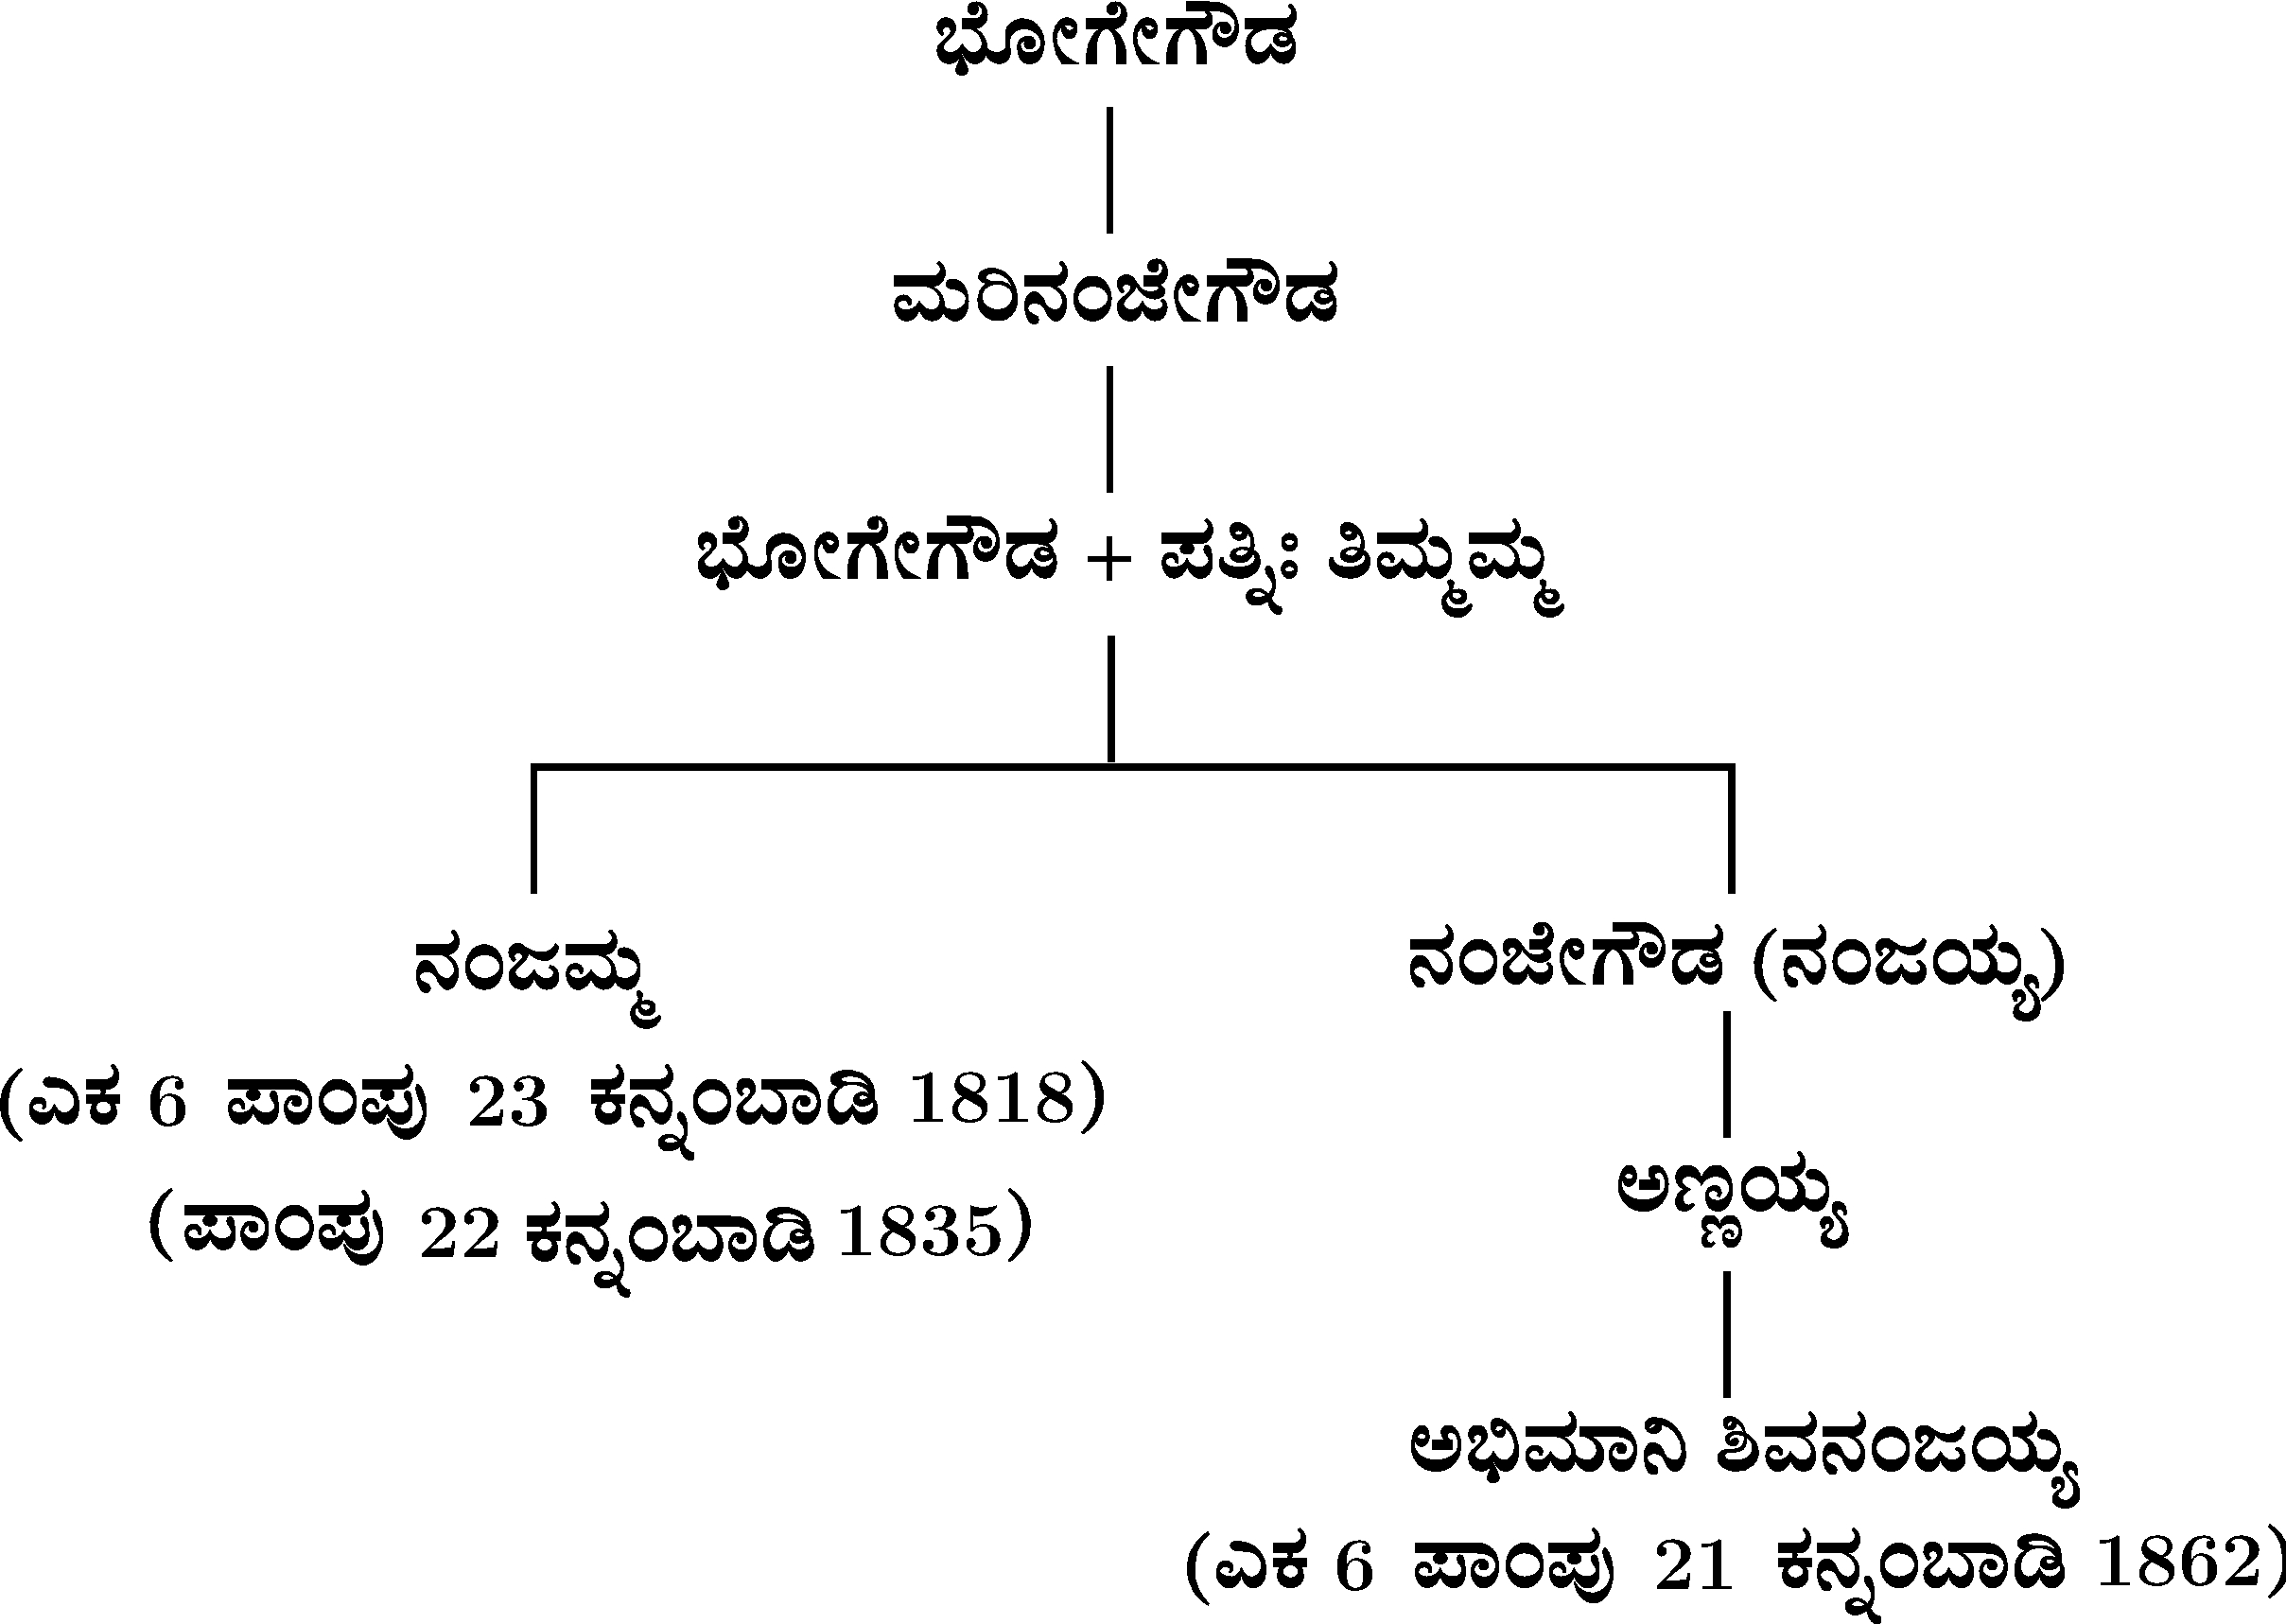
\includegraphics[scale=.9]{"images/chap5/chap5fig2.jpeg"}
\end{figure}

ಭೋಗೇಗೌಡನ ಪುತ್ರಿ ನಂಜಮ್ಮನು ಶ‍್ರೀ ಅಮ್ಮನವರಿಗೆ ರಂಗಮಂಟಪ ಮಾಡಿಸುತ್ತಾಳೆ. ಅ ಮಂಟಪಕ್ಕೆ ಮುಖಮಂಟಪ ಮಾಡಿಸುತ್ತಾಳೆ. ಶೀಮೆಗಳ ಮೇಲೆ ಬಂದ ಕಾಣಿಕೆಯಲ್ಲಿ ನಂಜಯ್ಯನು ಕನ್ನಂಬಾಡಿ ಗ್ರಾಮದ ಮಧ್ಯದಲ್ಲಿ ನೂತನ ದೇವಸ್ಥಾನವನ್ನು ಕಟ್ಟಿಸಿ, ಅವತಾರ ಭೇದವಾದ ಭೂತಗಣಕ್ಕೆ ಅಧಿಷ್ಠಾನ ದೇವತೆಯಾದ ಮಹಾಕಾಳಿ ಅಮ್ಮನವರು ಮತ್ತು ಸರಸ್ವತಿ ಅಮ್ಮನವರನ್ನು ಪರಿವಾರ ಸಮೇತವಾಗಿ ಪ್ರತಿಷ್ಠಾಪನೆ ಮಾಡಿಸುತ್ತಾನೆ. ಮಹಾಕಾಳಿ ಸರಸ್ವತಿ ಅಮ್ಮನವರ ದೇವಸ್ಥಾನಕ್ಕೆ ಹಿತ್ತಾಳೆ ವಡ್ನೆನಗ ಮಾಡಿಸಿ ಭಕ್ತಿ ಸೇವೆಯಾಗಿ ಅಲಂಕರಿಸುತ್ತಾನೆ. ಈತನು ತನ್ನ ವಂಶದ ಮೇಲೆ ಅಭಿಮಾನ ಹೊಂದಿದ್ದ ಕಾರಣಕ್ಕಾಗಿ ಶಿವನಂಜಯ್ಯನಿಗೆ ಅಭಿಮಾನಿ ಶಿವನಂಜಯ್ಯನೆಂಬ ಹೆಸರು ಬಂದಿರಬಹುದು. ಇತ್ತೀಚಿನವರೆಗೂ ಈ ಭಾಗದ ಗ್ರಾಮಗಳಲ್ಲಿ ದೇವಾಲಯವನ್ನು ಕಟ್ಟಿಸಲು ಹಣ ಬೇಕಾದಾಗ, ಮೆರೆಯುವ ದೇವರನ್ನು ಸುತ್ತಮುತ್ತಲ ಹಳ್ಳಿಗಳ ಮೇಲೆ ಮೆರವಣಿಗೆ ಮಾಡಿಸಿ ಬಂದ ಕಾಣಿಕೆಗಳನ್ನು ಕೂಡಿಸಿ ದೇವಾಲಯ ನಿರ್ಮಿಸುತ್ತಿದ್ದರು.

\textbf{ಚಂಗಿಕುಲ:} ಸಣ್ನೆ ನಾಡನ್ನು ಆಳುತ್ತಿದ್ದ ಸಾಮಂತ ಭರತೆಯ ನಾಯಕನನ್ನು ಚಂಗಿ ಕುಲಕಮಲ ಮಾರ್ತಾಂಡನೆಂದು ಕಂಬದಹಳ್ಳಿ ಶಾಸನವು ಬಣ್ಣಿಸಿದೆ.\endnote{ ಎಕ 7 ನಾಮಂ 29 ಕಂಬದಹಳ್ಳಿ 1174} ಇವನಿಗೆ ವೀರರಾಜೇಂದ್ರಹೊಯ್ಸಳ ಎಂಬ ಬಿರುದು ಇತ್ತು. ವೀರರಾಜೇಂದ್ರ ಎಂಬ ಬಿರುದು ಮೂಲತಃ ಚಂಗಾಳ್ವರದ್ದು. ನಂತರ ಇವರು ಹೊಯ್ಸಳರ ಅಧೀನರಾಗಿ ಆಳಿದರು. ಆದಕಾರಣ ಚಂಗಿ ಕುಲ ಎಂಬುದು ಚಂಗಾಳ್ವರ ಕುಲವನ್ನು ಸೂಚಿಸುತ್ತಿದೆ ಎಂದು ಹೇಳಬಹುದು. ಈ ಭಾಗದಲ್ಲಿ ಇತ್ತೀಚಿನವರೆಗೂ ಚೆಂಗಪ್ಪ ಎಂಬ ಹೆಸರನ್ನು ಗಂಗಡಿಕಾರ ಒಕ್ಕಲಿಗರು ಇಟ್ಟುಕೊಳ್ಳುತ್ತಿದ್ದರು. ಕೊಡಗು ಜಿಲ್ಲೆಯಲ್ಲಂತೂ ಚೆಂಗಪ್ಪ ಎಂಬ ಹೆಸರು ಸಾಮಾನ್ಯ. ಬಹುಶಃ ಇವರು ಈ ಚೆಂಗಿ ಕುಲದವರೇ ಇರಬಹುದೆಂದು ಹೇಳಬಹುದು.

\textbf{ಜೇಡರ ಕುಲ:} ಇಂದಿನ ದೇವಾಂಗ ಕುಲದ ಪ್ರಾಚೀನ ಮೂಲ ಹೆಸರು ಜೇಡರ, ಜಾಡರು. ಇವರನ್ನು ನೆಯ್ಗೆ ಕುಲದವರು, ಮಗ್ಗದವರು ಎಂದೂ ಕರೆಯಲಾಗುತ್ತದೆ. ನಾಗಮಂಗಲ, ಕೃಷ್ಣರಾಜಪೇಟೆ, ಪಾಂಡವಪುರ ಮತ್ತು ಮಂಡ್ಯ ತಾಲ್ಲೂಕುಗಳಲ್ಲಿ ಇವರ ಸಂಖ್ಯೆ ಹೆಚ್ಚಾಗಿದೆ. ದೇವಲಾಪುರ ಶಾಸನದಲ್ಲಿ ಜೇಡರ ಮೊಜ್ಜನ ಮಗ್ಗಕ್ಕೆ ಸಲ್ಲುವ ತೆರಿಗೆಯನ್ನು ಲಕ್ಷ್ಮೀಕಾಂತದೇವರ ವಸ್ತ್ರಕ್ಕೆ ಧಾರೆಯೆರೆದು ಕೊಡಲಾಗಿದೆ.\endnote{ ಎಕ 7 ನಾಮಂ 155 ದೇವಲಾಪುರ 1437} ಇದೇ ಮೊಜ್ಜನ ಮರೆ ಮಗ್ಗಕ್ಕೆ ಸಲ್ಲುವ 3 ಹಣವನ್ನು ಲಕ್ಷ್ಮೀಕಾಂತ ಸ್ವಾಮಿಯ ಮೈಭೋಗಕ್ಕೆ ಧಾರೆಯೆರೆದು ಕೊಡಲಾಗಿದೆ.\endnote{ ಎಕ 7 ನಾಮಂ 156 ದೇವಲಾಪುರ 1483} ಮೈಭೋಗ ಎಂದರೆ ಅಂಗಭೋಗ. ಇದರಲ್ಲಿ ವಸ್ತ್ರವೂ ಸೇರಿದೆ. ಜೇಡರದಾಸಿಮಯ್ಯನ ಮಗ ಕಾಟಿಗೌಡನು ಕೆರೆಯನ್ನು ಕಟ್ಟಿಸಿದಾಗ ಅದಕ್ಕೆ ಊರಿನ ಪ್ರಜೆಗಳು ಉಂಬಳಿಯನ್ನು ಬಿಟ್ಟರೆಂದೂ, ಕಾಟಿಗೌಡನು ಆ ಊರಿನ ಅಂದರೆ ಗಿಜೆಹಳ್ಳಿಯ ಮೇಳೇಶ್ವರ ದೇವರಿಗೆ ಗದ್ದೆಯನ್ನು ದತ್ತಿಯಾಗಿ ಬಿಟ್ಟನೆಂದೂ, ಅರಸಿಕೆರೆ ತಾಲ್ಲೂಕು ಗಿಜಹಳ್ಳಿ ಶಾಸನದಲ್ಲಿ ಹೇಳಿದೆ. ಜೇಡರ ದಾಸಿಮಯ್ಯನ ಹಾಗೂ ಅವನ ಮಗನ ಉಲ್ಲೇಖ ಇರುವ ಅಪರೂಪದ ಶಾಸನ ಇದಾಗಿದೆ.\endnote{ ಎಕ 10 ಅರ 222 ಗೀಜಹಳ್ಳಿ 1200} ಜೇಡಗೊತ್ತಳಿಯ ಉಲ್ಲೇಖ ಚಾಮರಾಜಪುರ(ಹಲುಕೂರು) ಶಾಸನದಲ್ಲಿಯೂ\endnote{ ಎಕ 10 ಅರ 97 ಜಯಚಾಮರಾಜಪುರ 12ನೇ ಶ.}, ಜೇಡದೆರೆಯ ಉಲ್ಲೇಖ ಕೆಲ್ಲಂಗೆರೆ ಶಾಸನದಲ್ಲಿಯೂ ಇದೆ.\endnote{ ಎಕ 10 ಅರ 160 ಕೆಲ್ಲಂಗೆರೆ 1161}

\textbf{ತೆನದಂಕ ಕುಲ:} ಶ‍್ರೀಮನ್​ ಮಹಾಪ್ರಧಾನ ಅಡ್ಡಾಯಿದದ ಹರಿಹರ ದಂಡನಾಯಕನನ್ನು \textbf{“ತೆನದಂಕ ಕುಲಾನ್ವಯ ಮೇರು, ತೆನದಂಕಕುಲ ಕಮಲ ಮಾರ್ತಾಂಡ”} ನೆಂದು ಬಸರಾಳು ಶಾಸನ ವರ್ಣಿಸಿದೆ.\endnote{ ಎಕ 7 ಮಂ 29 ಬಸರಾಳು 1234 ಮತ್ತು 27 ಬಸರಾಳು 1237} ಇವರು ಹರಿಹರ ದೇವರ ಪಾದಪದ್ಮಾರಾಧಕರಾಗಿದ್ದರು. ಇವನೂ ಇವನ ಸಹೋದರರೂ ಸೇರಿ ಬಸರಾಳಿನಲ್ಲಿ ಮಲ್ಲಿಕಾರ್ಜುನ ದೇವಾಲಯವನ್ನು ಮತ್ತು ಕೆರೆಗಳನ್ನೂ ಕಟ್ಟಿಸುತ್ತಾರೆ. ಇವರು ಶೈವಧರ್ಮಾವಲಂಬಿಗಳಾಗಿದ್ದರೆಂದು ಹೇಳಬಹುದು. ಅಂಕ ಎಂದರೆ ಯುದ್ಧ, ತೆನದಂಕ ಎಂಬ ಶಬ್ದ ಯುದ್ಧ ಸಂಬಂಧಿ ಅರ್ಥವನ್ನು ಹೊಂದಿರಬಹುದೇ ಎಂಬುದು ವಿಚಾರ ಮಾಡಬೇಕಾದ ಸಂಗತಿಯಾಗಿದೆ. ತೆನದಕ್ಕನ ಮಗ ಚೋಳಿಗ ಕಾದಿ ಮಡಿದನೆಂದು ಬಸರಾಳಿನ ಕೆರೆಯ ಹತ್ತಿರ ಇದ್ದ ಹರದನಹಳ್ಳಿ(ಬೇಚಿರಾಕ್​) ಗ್ರಾಮದ ಶಾಸನದಿಂದ ತಿಳಿದುಬರುತ್ತದೆ.\endnote{ ಎಕ 7 ಮಂ 33 ಹರದನಹಳ್ಳಿ 11-12ನೇ ಶ.} ತೆನದಕ್ಕ ಎಂಬುದು ಪುರುಷನ ಹೆಸರಾಗಿದ್ದು, ಇವನು ತೆನದಂಕ ವಂಶದವನಾಗಿರುವ ಸಾಧ್ಯತೆ ಇದೆ. ತೆನೆ ಎಂದರೆ ಕೋಟೆಯ ಮೇಲಿನ ರಚನೆಗಳು. ಇದಕ್ಕೆ ಕೋಟೆಯ ಅಗ್ರ, ಕಪಿಶೀರ್ಷ ತೊಂಡೆ ಎಂದೂ ಹೆಸರಿದೆ. ಇವರು ಕೋಟೆಯ ಮೇಲೆ ನಿಂತು ಯುದ್ಧ ಮಾಡುತ್ತಿದ್ದವರೇ ಎಂಬುದೂ ವಿಚಾರಾರ್ಹ. “ಹೊಮ್ಮದ ತೆನದಂಕರ ಕೇತ್ತಗೌಂಡನ” ಉಲ್ಲೇಖ ಕೆಂಪನಪುರ ಶಾಸನದಲ್ಲಿದ್ದು ಇದು ಅತ್ಯಂತ ಪ್ರಾಚೀನ ಉಲ್ಲೇಖವೆಂದು ಹೇಳಬಹುದು.\endnote{ ಎಕ 4 ಚಾನ 143 ಕೆಂಪನಪುರ} “ಕ್ರಿ.ಶ. 1165ರ ಹುಣಸೂರು ತಾಲ್ಲೂಕಿನ ತೊಂಡಾಳು ಶಾಸನದಲ್ಲಿ “ತೊಂಡೆಯಹಾಳ ತೆನದಂಕರ ಬೋಗೆಯ ಸಾವಂತನ ಮಗ ಹರದಗಾವುಂಡನು, ಕಾಳೆಯ ಸಾವಂತ ಗವುಡನೊಡಹುಟ್ಟಿದ ತಮುಉತ್ತಯ್ವರು (ಐದು ಜನ ಸಹೋದರರು) ಕೆರೆಯನ್ನು ಕಟ್ಟಿಸಿ, ಸೋಮೇಶ್ವರ ದೇವಾಲಯಕ್ಕೆ ದಾನ ನೀಡಿದರೆಂದು, ಚಾಮರಾಜನಗರದ ತಾಲ್ಲೂಕಿನ 12ನೇ ಶತಮಾನದ ಶಾಸನದಲ್ಲಿ ತೆನ್ನ ಪಕ್ಷದ ಚವುಡಗಾವುಂಡನ ಉಲ್ಲೇಖವಿದೆಯೆಂದು, ಇದೇ ತಾಲ್ಲೂಕಿನ ಬಾಗಳಿ ಶಾಸನದಲ್ಲಿ ತೊನದಕರ (ತೆನದಂಕರ) ಜಗಗೌಡನ ಉಲ್ಲೇಖವಿದೆಯೆಂದೂ, ತೆನದಂಕರ ಎಂಬುದು ತೆನೆ ಬೆಡಗಿಗೆ ಸಂಬಂಧಿಸಿದೆ” ಎಂದೂ ಸೂರ್ಯನಾಥ ಕಾಮತ್​ ಅವರು ಹೇಳಿದ್ದಾರೆ.\endnote{ ಸೂರ್ಯನಾಥ ಕಾಮತ್​, ಡಾ॥, ಒಕ್ಕಲುತನ ಮತ್ತು ಒಕ್ಕಲಿಗರು: ಇತಿಹಾಸ ಅನ್ವೇಷಣೆ, ಪುಟ 105} ತೆನದಕರ(ತೆನದಂಕ)ಕುಲದ ಪ್ರಾಚೀನ ಪ್ರಸ್ತಾಪ ಕ್ರಿ.ಶ.444ಕ್ಕೆ ಸೇರಿದ(ಎಂಟನೆಯ ಶತಮಾನದಲ್ಲಿ ಕೊರೆದ) ಹರಿವರ್ಮನ ತುಂಬಲ ಶಾಸನದಲ್ಲಿದೆ. ತೆನದಕರ ವಂಶವು ಶೌರ್ಯಕ್ಕೆ ಹೆಸರಾಗಿತ್ತು ಎಂದು ಹೇಳಿದೆ. ಮೈಸೂರು, ಕೆ.ಆರ್​.ನಗರ, ಮತ್ತು ಚಾಮರಾಜನಗರ ಶಾಸನಗಳಲ್ಲಿ ಈ ಮನೆತನದ ಉಲ್ಲೇಖ ಇರುವುದನ್ನು ಹೇಳಿದೆ.\endnote{ ನರಸಿಂಹಮೂರ್ತಿ, ಡಾ॥ ಎ.ವಿ., ಗಂಗ ಹರಿವರ್ಮನ ತುಂಬಲು ತಾಮ್ರಶಾಸನ, ಕರ್ನಾಟಕ ಪುರಾತತ್ವ, ಪುಟ 148} ಅಡ್ಡಾಯದ ಎಂಬುದು ಒಂದು ರೀತಿಯ ಆಯುಧ.

\textbf{ತೆಳರ (ತೆಳ್ಳರ) ಕುಲ:} ತೆಳರ ಕುಲತಿಲಕ ನಗರುರ ಸೋಮಯ್ಯನು ಹಡದ ಕ್ಷೇತ್ರದ ಬಂಕಿನಾಡನ್ನು ಆಳುತ್ತಿದ್ದನು. ಇವನ ವಂಶಜರು ಎರೆಯಂಗನ ಲೆಂಕರಾಗಿದ್ದರೆಂದು ಹೇಳಿದೆ. ಈ ಶಾಸನದಲ್ಲಿ ಒಂಭತ್ತು ಉಬ್ಬುಶಿಲ್ಪಗಳನ್ನು ಬಿಡಿಸಿದೆ.\endnote{ ಎಕ 7 ಮ 104 ಹಾಗಲಹಳ್ಳಿ 11ನೇ ಶ.} ತೆಳರಕುಲದ ಆದಿತ್ಯ ಗಾಮುಂಡನು ಬೊಪ್ಪಸಮುದ್ರದಲ್ಲಿ ತುರುಗೋಳಿನಲ್ಲಿ ಹೋರಾಡಿ ಮಡಿಯುತ್ತಾನೆ.\endnote{ ಎಕ 7 ಮ 103 ಹಾಗಲಹಳ್ಳಿ 11-12ನೇ ಶ.} ತೆಳ್ಳರಕುಲದ ಬೊಮ್ಮಣ್ಣನ ಉಲ್ಲೇಖವಿದೆ.\endnote{ ಎಕ 7 ಮ 113 ಬೊಪ್ಪಸಮುದ್ರ 1363} ಬೊಪ್ಪಸಮುದ್ರವನ್ನು ತೆಳ್ಳರ ವಂಶದವರ ಸಮ್ಮುಖದಲ್ಲಿ ಬಡವಾರಕುಲದ ಭಟ್ಟರಬಾಚಿಯಪ್ಪನ ಮಕ್ಕಳಿಗೆ ದತ್ತಿ ಹಾಕಿಕೊಡಲಾಗಿದೆ. ಶಾಸನದಲ್ಲಿ ಇವರ ವಂಶಾವಳಿಯನ್ನು ನೀಡಿದೆ. \textbf{ತೆಳ್ಳರ ವಂಶದ ತ್ರಿಭುವನಗಂಡ (ಶಿ)ವರಾ(ಯ)\textgreater  ದೇವಪ್ಪ\textgreater  ದಂಣ್ನು ಸಹದೇವ\textgreater  ದಂಣ್ನು ಮಾದಣ್ಣ\textgreater  ಕೊಮ್ಮಣ್ಣ. }\endnote{ ಎಕ 7 ಮ 110 ಬೊಪ್ಪಸಮುದ್ರ 1388} ತೆಳ್ಳರ ಕುಲದವರ ಪ್ರಸ್ತಾಪ ಬೊಪ್ಪಸಮುದ್ರ, ಹಾದಿರವಾಗಿಲು, ಹಾಗಲಹಳ್ಳಿ ಶಾಸನಗಳಲ್ಲೇ ಕಾಣಿಸಿಕೊಂಡಿದ್ದು, ಇವರು ಈ ಭಾಗದ ಮಾಂಡಲೀಕರಾಗಿ ಇವರು ಆಳ್ವಿಕೆ ನಡೆಸುತ್ತಿರಬಹುದೆಂದು ತೋರುತ್ತದೆ. \textbf{ಈ ಊರುಗಳಲ್ಲಿ ತೆಳ್ಳಾರಮ್ಮನೆಂಬ ಗ್ರಾಮದೇವತೆಯ ದೇವಾಲಯವೂ ಇದೆ.} ರಾಜರಾಜಚೋಳನ ಮಹಾಮಾತ್ಯ ಮತ್ತು ದಂಡನಾಯಕ ಅಪ್ರಮೇಯನನ್ನು ಕಲಿಯೂರು ಶಾಸನವು “ತೆಲ್ಲಕುಲ ತಿಲಕ” ಎಂದು ಕರೆದಿದೆ.\endnote{ ಎಕ 5 ತೀನಪು 220 ಕಲಿಯೂರು 1006} ಇವನು ತೆಲ್ಲ ಅಥವಾ ತೆಳ್ಳರ ಕುಲದವನೇ ಆಗಿದ್ದಾನೆ. ಜೊತೆಗೆ ಈತನು ತನ್ನ ಸಮುದಾಯದವರು ಹೆಚ್ಚಾಗಿರುವ ಮದ್ದೂರಿಗೆ ಸಮೀಪದ ಮಳೂರಿನಲ್ಲಿ ಅಪ್ರಮೇಯ ದೇವಾಲಯವನ್ನೂ ನಿರ್ಮಿಸಿದ್ದಾನೆ. ತೆಳನೂರ ವೀರಯ್ಯಗವುಡನು ಮಲ್ಲಿಕಾರ್ಜುನ ದೇವರಿಗೆ ಭೂಮಿಯನ್ನು ದತ್ತಿಬಿಟ್ಟಿದ್ದಾನೆ.\endnote{ ಎಕ 5 ತೀನಪು 81 ಬೆಟ್ಟದಹಳ್ಳಿ 1680}

ತೆಳರ(ತೆಳ್ಳರ) ಕುಲ-ತೆಲ್ಲಿಗರು ಎರಡೂ ಒಂದೇ ಅಥವಾ ಬೇರೆ ಬೇರೆಯೇ ಎಂಬುದು ವಿಚಾರಾರ್ಹ. “ಗ್ರಾಮ, ಪಟ್ಟಣಗಳಲ್ಲಿ, ಎಣ್ಣೆ ಉತ್ಪಾದನೆ ಮಾಡುವವರು ತೆಲ್ಲಿಗರು. ಇವರ ಇನ್ನೊಂದು ಹೆಸರು ಗಾಣಿಗರು, ತೆಲ್ಲಿಗರು ಮಧ್ಯಯುಗ ಕರ್ನಾಟಕದ ಬಹುಮುಖ್ಯ ಉತ್ಪಾದಕರು ವ್ಯಾಪಾರಿಗಳೂ ಆಗಿದ್ದರು.\endnote{ ಹಿರೇಮಠ್​, ಡಾ॥ ಬಿ.ಆರ್​. ಶಾಸನಗಳಲ್ಲಿ ಕರ್ನಾಟಕದ ವರ್ತಕರು, ಪುಟ 103-105} ಆದರೆ ಎಲ್ಲಿಯೂ ತೆಲ್ಲಿಗರಿಗೆ “ತೆಳರ” ಎಂಬ ಪದ ಪ್ರಯೋಗವನ್ನು ಮಾಡಿರುವುದು ಕಂಡು ಬರುವುದಿಲ್ಲ. ಅದೂ ಅಲ್ಲದೆ ತೆಲ್ಲಿಗರ ನಾಮವು ಸೆಟ್ಟಿ ಎಂಬ ವೃತ್ತಿನಾಮದಿಂದ ಅಂತ್ಯವಾಗುತ್ತದೆ.\endnote{ ಅದೇ, ಪುಟ 104}ಭೂಮಿಕಾರನಾದ \textbf{ತೆಳ್ಳರ ಕುಲದ} ಚಾಮಗಾವುಂಡನು ತಿಪ್ಪೂರು ತೀರ್ಥಕ್ಕೆ ಒಂದು ಕಲ್ಲಗಾಣವನ್ನು ಮಾಡಿಸಿಕೊಡುತ್ತಾನೆ. ಇವನನ್ನು ಶ್ರುತಕೀರ್ತಿದೇವರು ಮತ್ತು ಅನಾದಿಪಂಡಿತ ದೇವರ ಗುಡ್ಡನೆಂದು ಹೇಳಿದೆ.\endnote{ ಎಕ 7 ಮ 106 ಹಾಗಲಹಳ್ಳಿ 1700}\break ಚಾಮಗಾವುಂಡನ ವಂಶಾವಳಿಯು ಈ ಕೆಳಗಿನಂತಿದೆ. ತೆಳ್ಳರ ಕುಲದ ಎರೆಯಂಗ ಗಾವುಂಡ\textgreater ದೇವಗಾವುಂಡ\textgreater ಕಾವಗಾವುಂಡ\textgreater \break ಚಾಮಗಾವುಂಡ. ತೆಲ್ಲಿಗರು ವರ್ತಕ ಸಮುದಾಯದವರಾಗಿದ್ದು ಎಲ್ಲಿಯೂ ಗಾವುಂಡರಾಗಿರುವುದಿಲ್ಲ. ಗಾಣವನ್ನು ಮಾಡಿಸಿ ಕೊಟ್ಟಿರುವುದರಿಂದ ಇವನು ತೆಲ್ಲಿಗರ ಕುಲದವನಿರಬಹುದೆಂಬ ಅನುಮಾನ ಮೂಡುತ್ತದೆ.

\textbf{ನಾಯಿಂದರು(ನಾವಿದರು)(ವಾಲಗದವರು):} ಶ‍್ರೀರಂಗಪಟ್ಟಣದ ಸೀಮೆಯ ನಾಯಿಂದರಿಗೆ ಸುಂಕ, ಬೇಡಿಗೆಗಳನ್ನು ದತ್ತಿಯಾಗಿ ಬಿಡಲಾಗಿದೆ.\endnote{ ಎಕ 6 ಶ‍್ರೀಪ 36 ಶ‍್ರೀರಂಗಪಟ್ಟಣ 1438} ಚಂದಿಗಾಲು ಅಗ್ರಹಾರದಲ್ಲಿ ನಾಯಿಂದರ ಕೊಡುಗೆ ಹೊಲ ಇತ್ತೆಂದು ತಿಳಿದುಬರುತ್ತದೆ.\endnote{ ಎಕ 6 ಶ‍್ರೀಪ 25 ಶ‍್ರೀಪ 1430} ಈ ಶಾಸನದ ಕೆಳಗೇ ಮುಮ್ಮಡಿ ಕೃಷ್ಣರಾಜ ಒಡೆಯರೂ ಕೂಡಾ ಒಂದು ಶಾಸನವನ್ನು ಹಾಕಿಸಿ ಶ‍್ರೀರಂಗಪಟ್ಟಣ ನಗರ, ಚಂನಪಟ್ಟಣ ಕಂದ್ಯಾ (ಕಂದಾಯದ) ಊರು, ಉಭಯ ಅಷ್ಟಗ್ರಾಮ ಮುಂತಾದ ಗ್ರಾಮಗಳಲ್ಲಿ ಕೆಲಸದ ವಾಲಗದವರು, ಹದಿನೆಂಟು ಬಣಗಳಲ್ಲಿ ವಾಲಗವನ್ನು ಮಾಡಿದಾಗ ಅದಕ್ಕೆ ಕೆಲವು ಪ್ರತಿಫಲವನ್ನು ಪಡೆಯಲು ಅರ್ಹರೆಂದು ಶಾಸನ ಹಾಕಿಕೊಟಿದ್ದಾರೆ.\endnote{ ಎಕ 6 ಶ‍್ರೀಪ 37 ಶ‍್ರೀರಂಗಪಟ್ಟಣ 1801} ಇಲ್ಲಿ ನಾಯಿಂದರು, ವಾಲಗದವರು ಎಲ್ಲಾ ಒಂದೇ ಕುಲದ ಹೆಸರುಗಳಾಗಿವೆ. ಶ‍್ರೀರಂಗರಾಯನು, ಶ‍್ರೀರಂಗಪಟ್ಟಣ ಸೀಮೆಯ ನಾಯಕರುಗಳಿಗೆ ಕುಳಸುಂಕವನ್ನು ಮನ್ನಾ ಮಾಡಿದಾ, “ಯಿಂತ ತಪಿದವರು ನಾಇಂದರ ಮಕ್ಕಳು” ಎಂಬ ಶಾಪಾಶಯವನ್ನು ಪ್ರಯೋಗಿಸಿ, ಈ ಕುಲವನ್ನು ಕೀಳಾಗಿ ಕಂಡಿರುವುದನ್ನು ನೋಡಬಹುದು.\endnote{ ಎಕ 6 ಪಾಂಪು 237 ಸುಂಕಾತೊಂಡನೂರು 1550} ಧರ್ಮರಾಸಿ ಪಂಡಿತನ ಮಗ ಅಸಮಭಟ್ಟನು, ದೇವಡಿಗಗೆ(ದೇವಾಡಿಗನಿಗೆ) ದತ್ತಿಯನ್ನು ಬಿಟ್ಟನೆಂದು ತಿಳಿದುಬರುತ್ತದೆ.\endnote{ ಎಕ 6 ಪಾಂಪು 252 ತಿರುಮಲಸಾಗರ ಛತ್ರ 1125} ದೇವಾಡಿಗ ಎಂಬುದು ವಾಲಗದವರಿಗೆ ದಕ್ಷಿಣ ಕನ್ನಡ ಜಿಲ್ಲೆಯಲ್ಲಿ ಹೇಳುವ ಹೆಸರು.

\textbf{ಪರದರ ಕುಲ:} ಪರದರ ಕುಲದ ವರದಪ್ಪನ ಉಲ್ಲೇಖ ನಾಗಮಂಗಲ ತಾಲ್ಲೂಕು ಕೆಳಗೆರೆ ಶಾಸನದಲ್ಲಿದೆ.\endnote{ ಎಕ 7 ನಾಮಂ 59 ಕೆಳಗೆರೆ, 15ನೇ ಶ.} ಪರದ ಎಂಬುದು ಹರದ ಎಂಬುದರ ರೂಪಾಂತರ ಇರಬಹುದು. ಹರದ ಎಂದರೆ ವ್ಯಾಪಾರಿ. ಆದಕಾರಣ ಇವನು ವ್ಯಾಪಾರಿಗಳ ಕುಲಕ್ಕೆ ಸೇರಿರಬಹುದು. ಪರದರ ಕುಲದ ಹೊನ್ನೆಯ ನಾಯಕನ ಮಗ ವರದೆಯ ನಾಯಕನು (ವರದಪ್ಪ) ಭಟ್ಟಾರಕ ದೇವನ ಕೆಲ್ಲಂಗೆರೆಯನ್ನು ವರದರಾಜಪುರವೆಂಬ ಅಗ್ರಹಾರವನ್ನಾಗಿ ಮಾಡಿ ಅಲ್ಲಿ ಮಲ್ಲಿಕಾರ್ಜುನ ದೇವಾಲಯ ಮತ್ತು ಕೆರೆಗಳನ್ನು ಕಟ್ಟಿಸಿದನು.\endnote{ ಎಕ 7 ನಾಮಂ 58 ಕೆಳಗೆರೆ, 15ನೇ ಶ.}

\textbf{ಬಡವಾರ(ಬಡುವಾರ) ಕುಲ: } ಬಡುವಾರ/ಬಡವಾರ ಕುಲದ ದಾಮೋದರದೇವನ ಕುಮಾರ, ಕೀರ್ತಿದೇವನು ಮುಮ್ಮಡಿ ಬಲ್ಲಾಳನಿಂದ ದತ್ತಿಗಳನ್ನು ಪಡೆದನು.\endnote{ ಎಕ 7 ಮ 84 ಅರುವನಹಳ್ಳಿ 1316} ಮದ್ದೂರು ತಾಲ್ಲೂಕಿನ ಹಲವಾರು ಶಾಸನಗಳು ಬಡುವಾರ ಕುಲದ ಕೀರ್ತಿದೇವ ಹಾಗೂ ಅವನ ವಂಶದ ಭಟ್ಟರಬಾಚಿಯಪ್ಪ ಇವರ ವಂಶಾವಳಿ ಹಾಗೂ ಇತರ ವಿರವಗಳಿವೆ.\endnote{ ಎಕ 7 ಮದ್ದೂರು 85, 87, 93, 96, 102, 110} ಮದ್ದೂರು ತಾಲ್ಲೂಕು ಅರುವನಹಳ್ಳಿಯಲ್ಲಿ ಈ ಕುಲದವರ ಶಾಸನವಿರುವ ಆಂಜನೇಯ ದೇವಾಲಯದ ಅಂಗಳವನ್ನು ಇಂದಿಗೂ ಕೀರ್ತಿರಾಜನ ಅಂಗಳ ಎಂದೇ ಕರೆಯುತ್ತಾರೆ. ಬಡವಾರ ವಂಶೋದ್ಭವ ಪಾರಿಜಾತ ಕೀರ್ತಿದೇವ ತನೂಭವ ಬಾಚಿರಾಜನು, ಕೆರೆ, ಕಾಲುವೆಗಳನ್ನು ಮಾಡಿಸಿ, ಬಾಚಿರಾಜಪಟ್ಟಣವನ್ನು ಕಟ್ಟಿಸಿದನು. ಇವನು ಭೂಪಸ್ಥಾನಚಿ ರಂಜಿತ ಪ್ರಮುಖನಾಗಿದ್ದನೆಂದು ಶಾಸನ ಹೇಳಿದೆ.\endnote{ ಎಕ 7 ಮದ್ದೂರು 93 ಅರುವನಹಳ್ಳಿ 1358}

ಕೀರ್ತಿದೇವನ ಶಾಸನವನ್ನು ಪರಿಶೀಲಿಸಿದಾಗ, ಇವರು ಆನೆಗಳನ್ನು ಹಿಡಿದು ಪಳಗಿಸಿ ಹೊಯ್ಸಳರ ಸೇನೆಗೆ ಸರಬರಾಜು ಮಾಡುತ್ತಿದ್ದಿರಬಹುದು. ಅಥವಾ ಆನೆಗಳ ಸೇನೆಯ ಮುಖ್ಯಸ್ಥರಾಗಿರಬಹುದೆಂದು ಊಹಿಸಬಹುದು. ಗಜವೈದ್ಯವಿದ್ಯಾ ಪ್ರಸಿದ್ಧನಾದ ಜೈತೆಯನ ಹೆಂಡತಿಯ ಹೆಸರು \textbf{“ಬಡಿಯಬ್ಬೆ”} ಎಂದು ದೇಶಾಣಿ ಶಾಸನದಿಂದ ತಿಳಿದುಬರುತ್ತದೆ.\endnote{ ಎಕ 10 ಅರ 253 ದೇಶಾಣಿ 1139} ಈ ಬಡಿಯಬ್ಬೆಗೂ ಬಡವಾರ ಕುಲಕ್ಕೂ ಸಂಬಂಧ ಇರುವಂತೆ ತೋರುತ್ತದೆ. ಈ ಪ್ರದೇಶವನ್ನು ಬಡಗುನಾಡು ಎಂದು ಕರೆಯುತಿದ್ದು, ಬಡವಾರ ಕುಲದ ಹೆಸರು ಈ ನಾಡಿನ ಹೆಸರಿನಿಂದಲೂ ಬಂದಿರಬಹುದು.

\textbf{ಬಳಗಾರ ಕುಲ:} ಬಳಗಾರ ಕುಲದ ಬೀವಿಸೆಟ್ಟಿಯ ಮಗ ಬಮ್ಮಣ್ಣನು ಇಂಗಲಿಕನಕುಪ್ಪೆಯ ಸ್ವಯಂಭುದೇವರ ದೇವಾಲಯದಲ್ಲಿ ಎರಡು ಬಟ್ಟಾರ (ಪರಿವಾರದೇವತೆಗಳು) ದೇವಾಲಯವನ್ನು ಮಾಡಿಸಿ, ಉತ್ತರ ದಿಕ್ಕಿನ ಹಳ್ಳಕ್ಕೆ ಅಣೆಕಟ್ಟೆಯನ್ನು ಕಟ್ಟಿಸಿ, ಶೈವಯತಿಗಳಿಗೆ ದತ್ತಿಗಳನ್ನು ಬಿಡುತ್ತಾನೆ.\endnote{ ಎಕ 6 ಪಾಂಪು 252 ತಿರುಮಲಸಾಗರ ಛತ್ರ 1125} ಬಳೆಗಾರ ಕುಲವು ಜೈನಧರ್ಮದಲ್ಲಿ ಪ್ರಸಿದ್ಧ ಕುಲವಾಗಿದ್ದು ರನ್ನ ಕವಿಯು ಈ ಕುಲಕ್ಕೆ ಸೇರಿದವನು. ಮಂಡ್ಯ ಜಿಲ್ಲೆಯಲ್ಲಿ ಬೇಬಿ ಎಂಬ ಊರಿದೆ. ಇದು ಬೀವಿಸೆಟ್ಟಿ ಕಟ್ಟಿದ ಬೀವಿಸೆಟ್ಟಿಯ ಊರಾಗಿದ್ದು, ನಂತರ ಬೀವಿ\textgreater ಬೀಬಿ\textgreater ಬೇವಿ\textgreater ಬೇಬಿ ಆಗಿರುವ ಸಾಧ್ಯತೆ ಇದೆ. ಮೇಲುಕೋಟೆ ಬೆಟ್ಟದ ಕೆಳಗೆ ಬಳಘಟ್ಟ(ಬಳಿಗ) ಎಂಬ ಊರಿದೆ. ಇಲ್ಲಿ ನಿಸದಿ ಶಾಸನಗಳು ದೊರಕಿವೆ. ಬಳಗಾರ ಕುಲವು ಜೈನ ಧರ್ಮದಲ್ಲಿ ಬರುವ ಬಲಾತ್ಕರ ಗಣದ ಅನುಯಾಯಿಗಳ ಕುಲ ಎಂದು ಹಂಪನಾ ಅವರು ಹೇಳಿದ್ದಾರೆ.\endnote{ ನಾಗರಾಜಯ್ಯ, ಡಾ॥ ಹಂ.ಪ., ಶಾಸನಗಳಲ್ಲಿ ಯಾಪನೀಯ ಗಣಗಳು, ಚಂದ್ರಕೊಡೆ, ಪುಟ 155} ಆದರೆ ಅಯ್ಯಾವಳೆಯ ಬಳೆಗಾರ ಮಾರಿಶೆಟ್ಟಿಯು ತೆಂಕಲು ವ್ಯವಹಾರದಿಂದ ಬಂದು ಪೊಯ್ಸಳ ದೇವನನ್ನು ಕಂಡು ಅವನ ಕಾರುಣ್ಯದಿಂದ ಎಮ್ಮೆಸಂದಿಯನ್ನು ಪಡೆದು ಮಹಾಪ್ರಭುವಾಗಿದ್ದನೆಂದು, ಅವನ ಮಕ್ಕಳು ಬಸವಗಾವುಂಡ, ನಾಚಗಾವುಂಡ ಎಂದೂ ಇವರ ವಂಶದ ಪೆಮ್ಮಾಡಿಯು ಕೂಡಲೂರಿನಲ್ಲಿ ಹರಿಹರೇಶ್ವರ ದೇವಾಲಯವನ್ನು ನಿರ್ಮಿಸಿದನೆಂದು ತಿಳಿದುಬರುತ್ತದೆ.\endnote{ ಎಕ 9 ಬೇಲೂರು 225 ಕೂಡಲೂರು 1177-78} ಆದುದರಿಂದ ಇವರು ಶೈವರೇ ಎಂದು ಹೇಳಬಹುದು

\textbf{ಬೆಳ್ಳಿಯರ ಕುಲ:} ‘ನಗರೂರ ಬೆಳ್ಳಿಯರ’ ಪ್ರಸ್ತಾಪ ಶ‍್ರೀಪುರುಷನ ಹುಳ್ಳೇನಹಳ್ಳಿ ತಾಮ್ರ ಶಾಸನದಲ್ಲಿದೆ.\endnote{ ಎಕ 7 ಮಂ 14 ಹುಳ್ಳೇನಹಳ್ಳಿ 8ನೇ ಶ.} ಶ‍್ರೀಮನ್​ಮಹಾನಾಳ್ಪ್ರಭು ಬೆಳ್ಳಿಯರ ಕುಲತಿಲಕ, ಕಲಿದೇವರ ಪಾದಾರಾಧಕ ಕಲ್ಲ ಗವುಂಡನು, ತಮ್ಮಜ್ಜ ದಮ್ಮ ಗವುಂಡನ ಹೆಸರಿನಲ್ಲಿ ಕಿಕ್ಕೇರಿಯ ವೀಡಿಗೆ ಮುಖತಿಲಕದಂತಿದ್ದ, ಜಾಗನಕೆರೆಯಲ್ಲಿ ದಮ್ಮೇಶ್ವರ ದೇವಾಲಯವನ್ನು ನಿರ್ಮಿಸುತ್ತಾನೆ.\endnote{ ಎಕ 6 ಕೃಪೇ 69 ಜಾಗಿನಕೆರೆ 1242} ಈಗಲೂ ಕಿಕ್ಕೇರಿಯಲ್ಲಿ ಬೆಳ್ಳೇರು ಎಂಬ ಜಾತಿಯ ಜನರು ಇದ್ದಾರೆ. ಇವರುಗಳೂ ಕೂಡಾ ಗೌಡ ಎಂದು ಅಂತ್ಯವಾಗುವ ಹೆಸರುಗಳನ್ನು ಇಟ್ಟುಕೊಳ್ಳುತ್ತಾರೆ. ತಮ್ಮ ಕುಲದ ಲೋಹ ಬೆಳ್ಳಿ ಎಂದು ಹೇಳುತ್ತಾರೆ. ಇವರು ವಾಸಿಸುವ ಬೀದಿಗೆ ಬೆಳ್ಳೇರ ಕೇರಿ ಎಂದು ಹೇಳುತ್ತಾರೆ. ಇವರೇ ಬೆಳ್ಳಿಯರ ಕುಲದವರು. ಕಂಠೀರವ ನರಸರಾಜ ಒಡೆಯರು ಬೆಳ್ಳಿಕುಲೋದ್ಭವ ಚೆನ್ನವೀರಯ್ಯಗೌಡನವರ ಕುಮಾರ ದೊಡ್ಡಯ್ಯನವರಿಗೆ ಚನ್ನರಾಯಪಟ್ಟಣದ ಸೀಮೆಯನ್ನು ಕೊಟ್ಟಾಗ ಅದಕ್ಕೆ ಅವನು ಕಲ್ಲಕೋಟೆಯನ್ನು ಕಟ್ಟಿಸುತ್ತಾನೆ.\endnote{ ಎಕ 10 ಚರಾಪ 11 ಮತ್ತು 14 ಚನ್ನರಾಯಪಟ್ಟಣ 1648} ಈ ಕುಲದವರು ಗಂಗರ ಕಾಲದಿಂದ ಮೈಸೂರು ಅರಸರಕಾಲದವರೆಗೂ ಆಡಳಿತದಲ್ಲಿ ಭಾಗಿಯಾಗಿದ್ದರೆಂದು ಹೇಳಬಹುದು. ಬಡಗೆರೆನಾಡಿನ ಕಳಲ್​ತೂರಿನ ಬೆಳ್ಳಿಗವುಡನ ಮಗ ಬಿಟ್ಟಿಗವುಡನು ಸೋಮೇಶ್ವರದೇವರಿಗೆ ದತ್ತಿಬಿಟ್ಟನೆಂದು ಕ್ರಿ.ಶ. 1179ರ ಶಾಸನದಿಂದ ತಿಳಿದುಬರುತ್ತದೆ.\endnote{ ಶಾಸನ ಅಧ್ಯಯನ, ಸಂಪುಟ 4, ಕನ್ನಡ ವಿವಿ. ಹಂಪಿ, ಪುಟ 85}

ಬೆಳ್ಳಹಳ್ಳಿಯ ಪ್ರಸ್ತಾಪ ನಂಜನಗೂಡು ರಾಮಪುರ ತಾಲ್ಲೂಕಿನ ಶಾಸನದಲ್ಲಿದೆ.\endnote{ ಎಕ 3 ನಂಗೂ 159 ರಾಂಪುರ 1504} ಬೆಳಗುಂಬ, ಬೆಳ್ಳಿಕೆರೆ, ಬೆಳಗುಂದ, ಬೆಳವಾಡಿ ಇವೆಲ್ಲಾ ಬೆಳ್ಳಿಯನ್ನು ಪೂರ್ವಪದವಾಗಿ ಹೊಂದಿರುವ ಊರುಗಳ ಹೆಸರುಗಳು. ಬೆಳಗುಂಬದ ಹೆಸರು ಶಾಸನಗಳಲ್ಲಿ ಬೆಳ್ಳಿಗುಂಬ ಎಂದೇ ಇದೆ.\endnote{ ಎಕ 10 ಅರಸೀಕೆರೆ 175 ರಿಂದ 177 ಬೆಳಗುಂಬ} ಬೆಳ್ಳಿಯರ ಕುಲದ ಲೋಹ ಬೆಳ್ಳಿ ಆಗಿದ್ದಿರಬಹುದು. ಮರಸು ಒಕ್ಕಲಿಗರು ಮತ್ತು ಗಂಗಡಿಕಾರ ಒಕ್ಕಲಿಗರಲ್ಲಿ ಕೆಲವು ಮನೆತನದ ಲೋಹ ಕಂಚು. ಕಂಚಹಡವಳ ಎಂಬ ಹೆಸರಿನ ಉಲ್ಲೇಖವಿದೆ.\endnote{ ಎಕ 6 ಕೃಪೇ 42 ತೆಂಗಿನಘಟ್ಟ 1117} ಇದರಿಂದ ಈ ವಂಶದವರ ಲೋಹ ಕಂಚು ಆಗಿತ್ತೆಂದು ಹೇಳಬಹುದು. ಕೃಷ್ಣರಾಜಪೇಟೆ ತಾಲ್ಲೂಕಿನಲ್ಲಿ ಕಂಚಿನಕೆರೆ ಎಂಬ ಊರಿದೆ.\endnote{ ಎಕ 6 ಪಾಂಪು 99 ತೊಣ್ಣೂರು} ಸಂತೇಬಾಚಹಳ್ಳಿಯ ಹತ್ತಿರ ಕಂಚಿನಬೋರನ ಕಟ್ಟೆ ಎಂಬ ಒಂದು ಸಣ್ಣಕೆರೆಯೂ ಇದ್ದು, ಇದನ್ನು ಕಂಚುಕುಲದ ಬೋರ ಎಂಬುವವನು ಕಟ್ಟಿಸಿದನೆಂದು ಹೇಳುತ್ತಾರೆ.

\textbf{ಬೊಲರಕುಲ:} ಬೊಲರ ಕುಲದ ಗಂಗರಾಜರ ಕುಮಾರ ತಿರುಮಲರಾಜರು ವೃಂದಾವನಕ್ಕೆ ದತ್ತಿಯನ್ನು ಬಿಟ್ಟಿದ್ದಾರೆ. ಇದೊಂದು ರಾಜಮನೆತನವಿರಬಹುದು.\endnote{ ಎಕ 6 ಪಾಂಪು 218 ಹೊಸಹಳ್ಳಿ 1446}

\textbf{ಭೂಮಿಕಾರ ಬಾರಂದರ ಕುಲ:} ಮಂಡ್ಯ ಜಿಲ್ಲೆಯ ಶಾಸನಗಳಲ್ಲಿ ಹೆಚ್ಚಾಗಿ ಕಂಡುಬರುವ ಇನ್ನೊಂದು ಕುಲವೆಂದರೆ ಭೂಮಿಕಾರ ಬಾರಂದರ ಕುಲ. ಭೂಮಿಕಾರ ಎಂದರೆ, ಭೂಮಿಯ ಒಡೆಯ ಅಥವಾ ಜಮೀನುದಾರ ಎಂದು ಹೇಳಬಹುದು. ಆದರೆ ಬಾರಂದರ ಎಂಬುದನ್ನು ಅರ್ಥೈಸುವುದು ಕಷ್ಟ. ಬೆಂಗಳೂರು ಜಿಲ್ಲೆಯ ಚನ್ನಪಟ್ಟಣದ ಕಡೆ ಒಕ್ಕಲಿಗರಲ್ಲಿ ಬಂಧುಕಾರ ಎಂಬ ಉಪಪಂಗಡವಿದೆ. ಅದಕ್ಕೂ ಬಾರಂದರ ಕುಲಕ್ಕೂ ಸಂಬಂಧವಿದೆಯೇ ಎಂಬುದು ತಿಳಿದುಬರುವುದಿಲ್ಲ. ಅರಕೆರೆ ನಾಡನ್ನು ಆಳುತ್ತಿದ್ದ ಬೀರಗವುಂಡನು ಬಾರಂದರ ಕುಲಕ್ಕೆ ಸೇರಿದ್ದನು.\endnote{ ಎಕ 6 ಶ‍್ರೀಪ 113 ಅರಕೆರೆ 1108} ಭೂಮಿಕಾರ ಬಾರಂದರ ಕುಲದ ಚಿಕ್ಕಗೊಂಡನ ಮಗ ಕಾಚೈಯ್ಯ,\endnote{ ಎಕ 7 ಮ 98 ಬೆಲ್ಲೂರು 1122 (ಎಕ ಸಂಪಾದಕರು ಕಾಬೈಯ ಎಂದು ಓದಿದ್ದಾರೆ)}ಬೆಲ್ಲೂರ(ಬೆಳ್ಳೂರು) ಭೂಮಿಕಾರ ಬಾರಂದರ ಕಾಳಗೌಡನ ಮಗ ಬೀರಗೌಡ,\endnote{ ಎಕ 7 ಮ 97 ಬೆಲ್ಲೂರು 1369} ಇವರ ಉಲ್ಲೇಖ ಶಾಸನಗಳಲ್ಲಿದೆ.

ಬಾರಂದರ ಕುಲದ ಚಾಮಗವುಂಡನ ಮಗ ಬಿಣ್ನಾಂಡಿಯು ಮುದುಗೆರೆಯನ್ನು(ನಾಗಮಂಗಲ ತಾ. ಮುದಿಗೆರೆ) ಆಳುತ್ತಿದ್ದನು. ಅವನ ಮುತ್ತೆಯ, ಮುತ್ತಬ್ಬೆ,(ತಾತ, ಅಜ್ಜಿ) ಹಾಗೂ ಅವನ ಅವ್ವೆ ಚಾಮವ್ವೆಯರು ಸ್ವರ್ಗಸ್ಥರಾದಾಗ ಅವರ ಸ್ಮರಣಾರ್ಥ ಬಾರಂದೇಶ್ವರ ದೇವಾಲಯನ್ನು ನಿರ್ಮಿಸುತ್ತಾನೆ. ಇದು ಈ ಕುಲದವರ ದೇವರಿರಬಹುದು.\endnote{ ಎಕ 7 ನಾಮಂ 98 ಮುದಿಗೆರೆ 1139-40} ಸುಮಾರು ಇದೇ ಕಾಲದ ನಂಜನಗೂಡು ತಾ. ಕಾರ್ಯ ಶಾಸನದಲ್ಲಿ ಬಾರಂದರ ಕುಳಪತಿ ಕಾರೆಯದ ಹೆರ್ಮ್ಮಾಡಿ ಶಾವಂತ, ಬಾರಂದರ ಕುಳಪ್ರದೀಪ ವಿಭು ಹೆರ್ಮಾಡಿ ಗವುಂಡನ ಉಲ್ಲೇಖವಿದೆ.\endnote{ ಎಕ 3 ನಂಜನಗೂಡು 284 ಕಾರ್ಯ 12ನೇ ಶ.}

\textbf{ಮತ್ತಿಯರ ಕುಲ:} ತುರುಗೋಳಿನ ಶಾಸನದಲ್ಲಿ ಕದಂಬೆಹಳ್ಳಿಯ ಮತ್ತಿಯರ ಬಚಿಗವುಂಡನ ಮಗ ಕೇತಗವುಂಡನ ಉಲ್ಲೇಖವಿದೆ.\endnote{ ಎಕ 7 ಮವ 128 ಕದವಳ್ಳಿ 1183-84} ಮತ್ತಿಯರ ಎಂಬುದು ವೃಕ್ಷಸಂಬಂಧಿ ಕುಲನಾಮವೆಂದು ಹೇಳಬಹುದು. ಈ ಶಾಸನ ಇರುವ ಕದವಳ್ಳಿಯ ಹೆಸರೂ ವೃಕ್ಷಸಂಬಂಧಿಯಾಗಿದೆ.

\textbf{ಮಧುರೆಯದ ಕುಲ:} ಮಧುರೆಯದ ಕುಲದ ಕೆಂಪಗವುಂಡನ ಮಕ್ಕಳು ಗವುಡಿತಮ್ಮನ ಉಲ್ಲೆಖ ಗುತ್ತಲು ಶಾಸನದಲ್ಲಿದೆ.\endnote{ ಎಕ 7 ಮಂ 60 ಗುತ್ತಲು 1316}

\textbf{ಮಾಯಕಳಲಯಿಕ ಕುಲ:} ಮಾಯಕಳಲಯಿಕ ಕುಲದ ಸುಪುತ್ರ ರಾಮಸೆಟ್ಟಿಯು ಶಿವಾಲಯಕ್ಕೆ ಕಲ್ಲಿನ ಪಲ್ಲಕ್ಕಿಯನ್ನು ಮಾಡಿಸಿಕೊಟ್ಟನು.\endnote{ ಎಕ 6 ಪಾಂಪು 256 ಕಾಚೇನಹಳ್ಳಿ 13ನೇ ಶ.}

\textbf{ಮುಗಿಲಕುಲ:} ಕಬ್ಬಾಹು ನಾಡನ್ನು ಆಳುತ್ತಿದ್ದ ಮಹಾಸಾಮಂತ ಗಂಡನಾರಾಯಣ ಸೆಟ್ಟಿಯ ವಂಶಸ್ಥರು ತಾವು ಮುಗಿಲಕುಲ ಮಾರ್ತಾಂಡರೆಂದು ಹೇಳಿಕೊಂಡಿದ್ದಾರೆ. ಆದರೆ ಇವರು ವೀರಬಳಂಜು ಧರ್ಮವನ್ನು ಅನುಸರಿಸುತ್ತಿದ್ದವರು ಹಾಗೂ ವೇಳೆವಾಳಿಗಳು (ಗರುಡ) ಆಗಿದ್ದರು.\endnote{ ಎಕ 6 ಕೃಪೇ 77 ರಿಂದ 84 ಅಗ್ರಹಾರಬಾಚಹಳ್ಳಿ} ಗರುಡನಿಗೂ ಮುಗಿಲಿಗೂ(ಮೋಡ) ಅವಿನಾಭಾವ ಸಂಬಂಧವಿದೆ. ಗರುಡನು ಮುಗಿಲಿಗೆ ಒಡೆಯನಿದ್ದಂತೆ. ಆದುದರಿಂದ ಇವರು ತಮ್ಮನ್ನ ಮುಗಿಲಕುಲ ಮಾರ್ತಾಂಡರೆಂದು ಹೇಳಿಕೊಂಡಿದ್ದಾರೆಂದು ಊಹಿಸಬಹುದು. ಬೆಳ್ಳೂರಿನ ಪೆರುಮಾಳೆದೇವ ದಂಡನಾಯಕನೂ ಕೂಡಾ ಮೋಡಕುಲ/ಮೋಡೆಯಕುಲಕ್ಕೆ ಸೇರಿದವನು.\endnote{ ಎಕ 3 ಗುಂಡ್ಲುಪೇಟೆ 223 ಕಣ್ಣಾಗಾಲ, 152 ತ್ರಿಯಂಬಕಪುರ, 306 ಕೀಲಗೆರೆ, ಎಕ 12 ಕೊಳ್ಳೇಗಾಲ 30 ಸತ್ಯಾಗಾಲ} ಈ ಮೋಡಕುಲಕ್ಕೂ, ಗಂಡನಾರಾಯಣ ಸೆಟ್ಟಿಯ ಮುಗಿಲಕುಲಕ್ಕೂ ಏನಾದರೂ ಸಂಬಂಧವಿರಬಹುದು.

\textbf{ರಾಧೇಯ ಕುಲ ಅಥವಾ ಹರ್ಮ್ಯಕುಲ:} ಲಾಳನಕೆರೆ ಶಾಸನೋಕ್ತ ಅತ್ಯಮನಾಯಕನ ವಂಶದವರು ರಾಧೇಯಕುಲ ಅಥವಾ ಹರ್ಮ್ಯಕುಲದವರಾಗಿದ್ದರು. ಇವರನ್ನು ಸಂಭವರಾಯ ಕಾಡವರಾಯ ಕುಲಾನ್ವಯರು” ಎಂದು ಕರೆಯಲಾಗಿದೆ. ವೀರಬಲ್ಲಾಳನ ಸೇನೆಯಲ್ಲಿ ಇವರು ಎಡಗೈಯ ಸೇನಾನಾಯಕರಾಗಿದ್ದರು.\endnote{ ಎಕ 7 ನಾಮಂ 62 ಲಾಳನಕೆರೆ 1218} ಇವು ಮೂರೂ ಒಂದೇ ಕುಲದ ಪರ್ಯಾಯ ನಾಮಗಳು. ಚೋಳರ ಸಾಮಂತರಾಗಿ ಆಳುತ್ತಿದ್ದ ಶೇಂಗಣಿ ವಂಶದ ಶಂಭವರಾಯನ ಕುಲಕ್ಕೂ ಇದಕ್ಕೂ ಸಂಬಂಧವಿಲ್ಲ.\endnote{ ಎಪಿಗ್ರಾಫಿಯಾ ಕರ್ನಾಟಿಕಾ, ಸಂಪುಟ 7, ಪೀಠಿಕೆ}

\textbf{ವಾಜಿಕುಲ:} ನಾಗಮಂಗಲ ತಾ. ಲಾಳನಕೆರೆ ಶಾಸನೋಕ್ತ, ಮಧುಸೂದನ ದಂಡನಾಯಕನ ವಂಶದವರು ವಾಜಿಕುಲಕ್ಕೆ ಸೇರಿದವರು.\endnote{ ಎಕ 7 ನಾಮಂ 63 ಲಾಲನಕೆರೆ 1165} ಶಾಸನದಲ್ಲಿ ಇವರನ್ನು ಮನುಮಾರ್ಗರೆಂದು ಹೇಳಿಕೊಂಡಿದ್ದು, ಇವರನ್ನು ಹಾರುವರೆಂದು ಶಾಸನದಲ್ಲಿ ಹೇಳಿರುವುದರಿಂದ, ಇವರು ಸ್ಮಾರ್ತ ಬ್ರಾಹ್ಮಣ ಪಂಗಡದವರಾಗಿದ್ದರು. ವಾಜಿಕುಲವು ಜೈನಧರ್ಮದಲ್ಲಿ ಪ್ರಸಿದ್ಧವಾಗಿದೆ. ಜಿನಭಕ್ತ ಹುಳ್ಳಮಯ್ಯನೂ, ಶಿವಭಕ್ತ ಕಂಟಿಮಯ್ಯನೂ ಅಣ್ಣ ತಮ್ಮಂದಿರಂತೆ ಬಾಳಿದರೆಂದು, ಈ ಶಾಸನ ಮತೀಯ ಸೌಹಾರ್ದವನ್ನು ದಾಖಲಿಸಿದೆ ಎಂದು ಡಾ॥ ಹಂಪನಾ ಊಹಿಸಿದ್ದಾರೆ.\endnote{ ಅದೇ - ಪುಟ 432}ಮೈಸೂರು ಜಲ್ಲೆಯಲ್ಲಿ ವಾಜಿಮಂಗಲವೆಂಬ ಊರಿದ್ದು, ಇದು ವಾಜಿಕುಲ ಬ್ರಾಹ್ಮಣರ ಅಗ್ರಹಾರವಾಗಿದ್ದಿರಬಹುದು.

\textbf{ಸಂಕಿಯರ ಕುಲ:} ಕೃಷ್ಣರಾಜಪೇಟೆ ತಾಲ್ಲೂಕು ಕೈಗೋನಹಳ್ಳಿ ವೀರಶಾಸನವು ಮಾರಗೊಂಡ(ಗವುಡ) ಹಾಗೂ ಅವನ ಪುತ್ರರನ್ನು ಸಂಕಿಯರ ಕುಲತಿಲಕರೆಂದು ಕರೆದಿದೆ. ಇವರು ಯುದ್ಧದಲ್ಲಿ ಹೋರಾಡಿ ಮಡಿಯುತ್ತಾರೆ.\endnote{ ಎಕ 6 ಕೃಪೇ 70 ಕೈಗೋನಹಳ್ಳಿ 12ನೇ ಶ.}ಪಟ್ಟಣಸ್ವಾಮಿ ಹಳ್ಳಿಯ ಸಂಕಿಯರ ಕುಲದ ಸಾಮಂತನ ಸುಪುತ್ರ ಮಲ್ಲಯ್ಯ ಹೊಯ್ಸಳಾನ್ವಯ ವೀರನಾಗಿದ್ದು ಊರಳಿವಿನಲ್ಲಿ ಹೋರಾಡಿ ಸ್ವರ್ಗಸ್ಥನಾಗುತ್ತಾನೆ.\endnote{ ಎಕ 6 ಪಾಂಪು 258 ಪಟ್ಟಸೋಮನಹಳ್ಳಿ 1273} ಬಸವಕವಿಯ ಭೀಮಪುರಾಣದಲ್ಲಿ ಸಂಕೀ ದೇವನ ಪ್ರಸ್ತಾಪವಿದೆ.

\textbf{ಸೂತಕುಲ:} ಸೂತ ನರಸಿಂಗಯ್ಯ, ಮತ್ತು ಪಟ್ಟಸಾಹಣಿ ಮಹದೇವಣ್ಣ ಇವರುಗಳಿಗೆ ದೀರ್ಘಾಯುವಾಗಲೆಂದು ಕೂಸ ಎರೆಯಣ್ಣನು ಕಲಿದೇವರಿಗೆ ದತ್ತಿ ಬಿಟ್ಟನೆಂದು ಕಸಲಗೆರೆ ಶಾಸನದಲ್ಲಿ ಹೇಳಿದೆ.\endnote{ ಎಕ 7 ನಾಮಂ 168 ಕಸಲಗೆರೆ} ಪಟ್ಟಸಾಹಣಿ ಎಂದರೆ ಕುದುರೆಗಳ ಸೈನ್ಯದ ಒಡೆಯ. ಸೂತ, ಸೂತರು ಎಂದರೆ ಕುದುರೆಯನ್ನು ಕಟ್ಟಿದ ರಥವನ್ನು ಓಡಿಸುವವರು. ಮಹಾಭಾರತದ ಕರ್ಣನು ಸೂತಕುಲದ ರಾಧೇಯನ ಬಳಿ ಬೆಳೆದನೆಂದು ಹೇಳಿದೆ. ಸೂತ ನರಸಿಂಗಯ್ಯನೂ, ಕುದುರೆಗಳ ಸೇನೆಯ ಒಡೆಯ ಮಹದೇವಣ್ಣನ ಬಳಿ ರಥ ಓಡಿಸುವವರ ಮುಖ್ಯಸ್ಥನಾಗಿದ್ದನೆಂದು ಹೇಳಬಹುದು.

\textbf{ಹಳ್ಳಿಕಾರ (ಹಳಿಕಾರ):} ಹಳಿಕಾರ ಲಕ್ಕಣ್ಣನಾಯಕರ ಮಕ್ಕಳು ಚಿಕ್ಕಅಲ್ಲಪ್ಪನಾಯಕನು ದೇವಲಾಪುರದ ನಾಯಕ\-ನಾಗಿದ್ದನು.\endnote{ ಎಕ 7 ನಾಮಂ 158 ದೇವಲಾಪುರ 1472} ಹಳ್ಳಿಕಾರ ಸಮಾಜವು ಮಂಡ್ಯ ಜಿಲ್ಲೆಯ ಮದ್ದೂರು, ನಾಗಮಂಗಲ ತಾಲ್ಲೂಕುಗಳಲ್ಲಿ ಹೆಚ್ಚಾಗಿರುವುದು ಕಂಡುಬರುತ್ತದೆ. ಜಿಲ್ಲಾ ಕೇಂದ್ರವಾದ ಮಂಡ್ಯದಲ್ಲಿ ಇವರ ಒಂದು ಸಂಘವೂ ಇದೆ. ಹಳ್ಳಿಕಾರ ಎಂಬ ಹಸು ಮತ್ತು ಎತ್ತುಗಳ ತಳಿಯು ದಕ್ಷಿಣ ಕರ್ನಾಟಕದ ಬಯಲು ಸೀಮೆಯಲ್ಲಿ ಪ್ರಖ್ಯಾತವಾಗಿದೆ.

\textbf{ಹೊಲೆಯ:} ಹೊಲೆಯರು ಸಮಾಜದ ಪ್ರಮುಖ ಅಂಗವಾಗಿದ್ದರು. ಆದರೂ ಅವರು ಊರಿನಿಂದ ಪ್ರತ್ಯೇಕವಾಗಿರುವ ಕೇರಿಯಲ್ಲಿ ವಾಸಿಸುತ್ತಿದ್ದರು. ಇವರಿಗೆ ಪ್ರತ್ಯೇಕ ಕೆರೆ ಕಟ್ಟೆಗಳಿದ್ದವು. ಇವರನ್ನು ಪಂಚಮರೆಂದು ಕರೆಯ\-ಲಾಗಿದೆ. ತೊಣ್ಣೂರು ಶಾಸನದ ಶಾಪಾಶಯದಲ್ಲಿ “ಈ ಧರ್ಮಮಂ ಕಿಡಿಸಿದವಂ ಪಂಚಮ ಮಾಡಿದ ಪಾಪ” ಎಂದು ಹೇಳಿದೆ.\endnote{ ಎಕ 6 ಪಾಂಪು 80 ತೊಣ್ಣೂರು 1177} ಅಳೀಸಂದ್ರ ಶಾಸನದಲ್ಲಿ ಹೊಲೆಗೆರೆ ಮತ್ತು ಹೊಲೆಗೇರಿಯ ಪ್ರಸ್ತಾಪವಿದೆ.\endnote{ ಎಕ 7 ನಾಮಂ 72 ಅಳೀಸಂದ್ರ 1183} ಹೊಲೆಯರ ಹಳ್ಳದಸಾಗರ\endnote{ ಎಕ 10 ಚರಾಪ 40 ದಿಂಡಗೂರು 1209} ಹೊಲೆಗೆರೆಯ ಕೋಡಿ\endnote{ ಎಕ 10 ಚರಾಪ 70 ಕೆಂಬಾಳು 1235} ಪ್ರಸ್ತಾಪಗಳನ್ನು ಶಾಸನಗಳಲ್ಲಿ ಕಾಣಬಹುದು. ಹೊಲೆಗೇರಿ ಮತ್ತು ಹೊಲೆಗಟ್ಟೆಗಳು ಆಗಿನ ಕಾಲದಿಂದಲೂ ಅಸ್ತಿತ್ವದಲ್ಲಿದ್ದವು ಎಂದು ಹೇಳಬಹುದು. ಹೊಲೆಯರ ಜೀವದ ಸಾಲಿನ... ಬಾವಲಯಣವನ್ನು ಕೂಸ ಎರೆಯಣ್ಣನು ದತ್ತಿಯಾಗಿ ಬಿಟ್ಟನೆಂದು ಹೇಳಿದೆ. ಇದು ಬಹುಶಃ ಹೊಲೆಯರ ಮೇಲೆ ಹಾಕಿದ್ದ ತೆರಿಗೆಯಾಗಿದ್ದಿರಬಹುದು.\endnote{ ಅದೇ} ಹೊಲೆಯರ ಮೇಲೆ ಹಾಕುತ್ತಿದ್ದ “ಹೊಲೆದೆರೆಯ” ವಿಚಾರ ವೈದ್ಯನಾಥಪುರ ಶಾಸನದಲ್ಲಿದೆ.\endnote{ ಎಕ 7 ಮ 71 ವೈದ್ಯನಾಥಪುರ 12-13ನೇ ಶ.} ಹೊಲೆಯರ ಸುಂಕವನ್ನು ಮನ್ನಾ ಮಾಡಿರುವ ವಿಚಾರವನ್ನು ಬೀಚನಹಳ್ಳಿ ಶಾಸನದಿಂದ ತಿಳಿಯಬಹುದು.\endnote{ ಎಕ 7 ನಾಮಂ 18 ಬೀಚನಹಳ್ಳಿ 16 ನೇ ಶ.} ಕಬ್ಬಿಲರ ಹದಿಕೆ, ಹೊಲೆಯರ ಹದಿಕೆಗಳ ಪ್ರಸ್ತಾಪ ಚನ್ನರಾಯಪಟ್ಟಣ ತಾಲ್ಲೂಕಿನ ಶಾಸನದಲ್ಲಿದೆ.\endnote{ ಎಕ 10 ಚರಾಪ 126 ಪುರ 1235}

ಇವರನ್ನು ಕೀಳಾಗಿ ಕಂಡರೂ, ಇವರಿಗೆ ಅಂದಿನ ಸಮಾಜದಲ್ಲಿ ಜವಾಬ್ದಾರಿಯುತ ಸ್ಥಾನವನ್ನು ನೀಡಿರುವುದೂ ಕಂಡುಬರುತ್ತದೆ. \textbf{ಹೆಬ್ಬಹೊಲೆಯ ಮಂಡನಯಾಕ ಎಂಬುವವನು ಗುತ್ತಲಿನಲ್ಲಿ ನಡೆದ ವ್ಯವಹಾರಕ್ಕೆ ಸಾಕ್ಷಿಯಾಗಿರುವುದನ್ನು ನೋಡಬಹುದು}.\endnote{ ಎಕ 7 ಮಂ 60 ಗುತ್ತಲು 1316} ಈತನು ಹೊಲೆಯರ ಕುಲದ ಮುಖಂಡನಿರಬಹುದೆಂದು ಹೇಳಬಹುದು. ಯಾವುದೋ ಕೊಡುಗೆಗೆ\break ಇತರ ಸಾಕ್ಷಿಗಳ ಜೊತೆಗೆ “ಹೊಲೆ ಅಷವಂ” ಸಾಕ್ಷಿಯಾಗಿದ್ದಾನೆ.\endnote{ ಎಕ 3 ನಂಗೂ 320 ಗಟ್ಟವಾಡಿ 10ನೇ ಶ.} ವೀರನರಸಿಂಹನ ಕಾಲದ ನಂಜನಗೂಡು ತಾಲ್ಲೂಕು, ದಾಸನೂರು ಶಾಸನದಲ್ಲಿ “ಹೊಲೆಯರಸ...ಕವನ ಬಂಕ ಕಾವ ಇಂತೀ ಸಮಸ್ತ ಪ್ರಜೆಯು ಒಂಡಂಬಟ್ಟು ಶ‍್ರೀ ವಿಶ್ವನಾಥದೇವರಿಗೆ ಒಂದು ದೀವಿಗೆ, ಒಂದು ಉಪಾರಕೆ ಬಿಟ್ಟ ಭೂಮಿ” ಎಂದು ಹೇಳಿದೆ.\endnote{ ಎಕ 3 ನಂಗೂ 290 ದಾಸನೂರು 1278} ಊರಿನ ಆಡಳಿತವನ್ನು ನಡೆಸುವ ಸಂಸ್ಥೆಯಾದ “ಪ್ರಜೆ”ಯಲ್ಲಿ ಹೊಲೆಯರಸ ಅಂದರೆ ಹೊಲೆಯರ ಮುಖಂಡನಿಗೂ ಒಂದು ಸ್ಥಾನವಿತ್ತು ಎಂಬುದು ವಿಚಾರಾರ್ಹ.

\textbf{ಹದಿನೆಂಟು ಸಮಯ:} ಸಮಯ ಎಂದರೆ ಧರ್ಮ ಅಥವಾ ಸಿದ್ಧಾಂತ(ಪಂಥ) (ಉದಾಗೆ. ಜಿನಸಮೆಯ, ಶಿವಸಮಯ) ಹದಿನೆಂಟು ಸಮಯ ಎಂದರೆ ಹದಿನೆಂಟು ಧರ್ಮಗಳು ಅಥವಾ ಸಿದ್ಧಾಂತಕ್ಕೆ ಸೇರಿದ ಸಮುದಾಯದವರು ಎಂಬ ಅರ್ಥ ಬರುತ್ತದೆ. ಹೊಯ್ಸಳರ ಕಾಲದಲ್ಲಿ ಈ ಪದಪ್ರಯೋಗ ಇರುವುದರಿಂದ ಆಗ ಹದಿನೆಂಟು ಸಮಯಗಳು ಇದ್ದಿರಬಹುದು. “ಯಂ ಶೈವಸಮುಪಾಸತೆ” ಎಂಬ ಶ್ಲೋಕದಲ್ಲಿ ಕೆಲವು ಧರ್ಮಗಳು ಅಥವಾ ಸಿದ್ಧಾಂತಗಳನ್ನು ಹೇಳಿದೆ.

ಅಯ್ಯಾ ಪೊಳಲ್​ನ ವರ್ತಕರು ಹದಿನೆಂಟು ಸಮಯಕ್ಕೂ ಬೇಕಾದವರಾಗಿದ್ದರೆಂದು ಹೇಳಿದೆ.\endnote{ ಎಕ 7 ಮವ 51 ದನಗೂರು 13ನೇ ಶ.} ದೇವರಿಗೆ ಬಿಟ್ಟ ದತ್ತಿಯು ಹದಿನೆಂಟು ಸಮಯದವರಿಗೂ ಸಲ್ಲುತ್ತದೆ ಎಂದು ಹೇಳಿದೆ.\endnote{ ಎಕ 7 ಮವ 54 ಮಾರೆಹಳ್ಳಿ 13ನೇ ಶ.} ಹದಿನೆಂಟು ಸಮಯದವರು ಕೂಡಿ ಕನ್ನಂಬಾಡಿಯ ಗೋಪಾಲಕೃಷ್ಣ ದೇವಾಲಯವನ್ನು ಜೀರ್ಣೋದ್ಧಾರ ಮಾಡಿ ದತ್ತಿಬಿಟ್ಟರೆಂದು ತಿಳಿದುಬರುತ್ತದೆ.\endnote{ ಎಕ 7 ಪಾಂಪು 31 ಕನ್ನಂಬಾಡಿ 14ನೇ ಶ.} ಸಣ್ಣೇನಹಳ್ಳಿ ವೀರಗಲ್ಲಿನಲ್ಲಿ ಹದಿನೆಂಟು ಸಮಯವನ್ನು, ಅರವತ್ತೊಕ್ಕಲಿನ ಜೊತೆ ಉಪಯೋಗಿಸಿರುವುದರಿಂದ ಇದೊಂದು ಸಂಘವಾಗಿರಬಹುದು.\endnote{ ಎಕ 10 ಚರಾಪ 27 ಸಣ್ಣೇನಹಳ್ಳಿ 1289} ಎಪಿಗ್ರಾಫಿಯಾ ಕರ್ನಾಟಿಕಾ ಸಂಪಾದಕರೂ ಇದನ್ನು ಸಂಘ ಎಂದೇ ಹೇಳಿದ್ದಾರೆ. ಶಾಪಾಶಯವನ್ನು ಹೇಳುವಾಗ ಈ ಧರ್ಮವನ್ನು ಅಳಿದವನ್ನು ಹದಿನೆಂಟು ಸಮಯಕ್ಕೆ ದ್ರೋಹಿ ಎಂದು ಪುರ ಶಾಸನದಲ್ಲಿ ಹೇಳಿದೆ.\endnote{ ಎಕ 10 ಚರಾಪ 126 ಪುರ 1259} ಹದಿನೆಂಟು ಕಾಲ್ಪನಿಕ ಸಂಖ್ಯೆಯೇ, ಅಥವಾ ಹದಿನೆಂಟು ಸಮಯಗಳು ಇದ್ದವೆ ಎಂಬುದು ಪರಿಶೀಲಿಸಬೇಕಾದ ವಿಷಯ.

\textbf{ಮುದಜಾತಿ ಗ್ರಾಮ:} ಮಾರೆಹಳ್ಳಿಯನ್ನು ಜಾತಿಗ್ರಾಮ, ಸಕಲ ಜಾತಿ ಗ್ರಾಮ, ಮುದಜಾತಿ ಗ್ರಾಮ ಎಂದು ಕರೆಯಲಾಗಿದೆ.\endnote{ ಎಕ 7 ಮವ 62 ಮಾರೆಹಳ್ಳಿ 1148, 71 ಮಾರೆಹಳ್ಳಿ 1406} ಮಾರೇನಹಳ್ಳಿಯು ಅಗ್ರಹಾರವಾಗಿದ್ದು, ಇಲ್ಲಿ ಎಲ್ಲ ಜಾತಿಯ ಜನರು ವಾಸವಾಗಿದ್ದರೇ ಅಥವಾ ಗ್ರಾಮದ ಹೆಸರೇ ಈ ರೀತಿ ಇತ್ತೆ ಎಂಬುದು ಪ್ರಶ್ನಾರ್ಹವಾಗಿ ಉಳಿಯುತ್ತದೆ.\endnote{ ಎಪಿಗ್ರಾಫಿಯಾ ಕರ್ನಾಟಿಕಾ, ಸಂಪುಟ 7, ಪುಟ \engfoot{liv}} ಮುದುಗೂರು, ಮುದವಾಡಿ, ಮುದುಡಿ, ಮುದುಗುಂದೂರುಗಳ ಉಲ್ಲೇಖ ನಮಗೆ ಶಾಸನಗಳಲ್ಲಿ ದೊರೆಯುತ್ತದೆ. ಮುದಬೋವ, ಮುದಗಾವುಂಡ ಎಂಬ ಹೆಸರುಗಳೂ ಇವೆ. ಮುದವಿಡಿಯ ಸೀಮೆ ಎಂಬ ಆಡಳಿತ ವಿಭಾಗದ ಉಲ್ಲೇಖ ಚಿಕ್ಕಗಂಡಸಿ ಶಾಸನದಲ್ಲಿದೆ.\endnote{ ಎಕ 10 ಅರ 206 ಚಿಕ್ಕಗಂಡಸಿ 1535} ಮೇಲೆ ಪ್ರಯೋಗಿಸಲಾದ ಮುದ ಎಂಬ ಶಬ್ದಕ್ಕೂ, ಮುದಜಾತಿಗ್ರಾಮ ಪ್ರಯೋಗಕ್ಕೂ ಏನಾದರೂ ಸಂಬಂಧವಿದೆಯೇ ಎಂಬುದನ್ನೂ ಪರಿಶೀಲನಾರ್ಹ.

\textbf{ಇತರ ಜಾತಿಗಳು:} ಬ್ರಾಹ್ಮಣರು ಅಗ್ರಹಾರದಲ್ಲಿ ಪಡೆದ ವೃತ್ತಿಗಳನ್ನು ಶೂದ್ರರಿಗೆ ಮಾರಿದರೆ, ಅವರನ್ನು ಬ್ರಾಹ್ಮಣಿಕೆ\-ಯಿಂದ ಬಹಿಷ್ಕರಿಸಲಾಗುತ್ತಿತ್ತು ಎಂಬ ವಿಚಾರ ತಿಳಿದುಬರುತ್ತದೆ.\endnote{ ಎಕ 7 ಮವ 139 ಸುಜ್ಜಲೂರು 1473} ದಾನವನ್ನು ಅಪಹರಿಸಿದವನು, ಅಪಹರಿಸಲು ಸಹಕಾರಿಯಾದವನು ಕಿರಾತ, ಮ್ಲೇಚ್ಛ, ಚಂಡಾಲ, ಚಮ್ಮಕಾರರ(ಚರ್ಮಕಾರರ) ಜಾತಿಯಲ್ಲಿ ಜನಿಸುತ್ತಾನೆಂದು ತೊಣ್ಣೂರು ದೇವಾಲಯದಲ್ಲಿರುವ ಕ್ರಿ.ಶ.1722ರ ತಾಮ್ರ ಶಾಸನದಲ್ಲಿ ಹೇಳಿದೆ.\endnote{ ಎಕ 6 ಪಾಂಪು 91 ತೊಣ್ಣೂರು 1722} ಈ ಜಾತಿಗಳು ಬಹಳ ಕೀಳು ಎಂಬ ಭಾವನೆ ಇತ್ತು ಎಂದು ಹೇಳಬಹುದು.

ಅಗ್ರಹಾರವನ್ನು ದತ್ತಿಯಾಗಿ ನೀಡಿದಾಗ, \textbf{“ಒಕ್ಕಲುಮಕ್ಕಳು ಸಹ ಶೂದ್ರಪ್ರಜೆ ನಾನಾ ಜಾತಿಯಾದ ಬಿನುಗು ಪ್ರಜೆಯನೂ ಆಳಿಕೊಂಡು ಬಹಿರಿ”} ಎಂದು ಹೇಳಿದೆ.\endnote{ ಎಕ 7 ಮವ 106 ಮುಟ್ಣಹಳ್ಳಿ 1506} ಇದು ಅಗ್ರಹಾರದ ಪ್ರಜೆಗಳಿಗೆ, ಅಗ್ರಹಾರದ ಒಡೆಯರಿಗೆ ಅಗ್ರಹಾರದಲ್ಲಿ ವಾಸಿಸುವ ಇತರ ಜಾತಿ ಸಂಘಗಳ ಮೇಲೆ ಅಧಿಕಾರವಿತ್ತು ಎಂಬುದನ್ನು ತೋರಿಸುತ್ತದೆ. ಶೂದ್ರರನ್ನು ಹೊರತುಪಡಿಸಿ ಇತರ ಜನಾಂಗದವರಿಗೆ ಬಿನುಗು ಪ್ರಜೆಗಳೆಂದು ಹೇಳಿರಬಹುದು. ಬಿನುಗುದೆರೆಯ ಪ್ರಸ್ತಾಪ ಅನೇಕ ಶಾಸನಗಳಲ್ಲಿದೆ.

ಮಂಡ್ಯ ಜಿಲ್ಲೆಯ ಶಾಸನಗಳಲ್ಲಿ, ಕುಂಬಾರರ ಜಾತಿಯ ಪ್ರಸ್ತಾಪವಿದೆ. ಶ‍್ರೀರಂಗಪಟ್ಟಣದ ಗಂಗಾಧರೇಶ್ವರ ದೇವಾಲಯದಲ್ಲಿರುವ ತಮಿಳುನಾಡಿನ ಪುರಾತನರ ವಿಗ್ರಹಗಳ ಕೆಳಗೆ ಮನಕೋಜ ಕುಳಾಳರು, ಶ‍್ರೀನೀಲಕಂಠ ಕುಂಬಾರರು ಎಂಬ ಹೆಸರುಗಳಿವೆ.\endnote{ ಎಕ 6 ಶ‍್ರೀಪ 28 ಶ‍್ರೀರಂಗಪಟ್ಟಣ 18ನೇ ಶ.} “ಕುಂಭಕಾರ ತಟಾಕಾಂತ”\endnote{ ಎಕ 6 ಕೃಪೇ 71 ಕೈಗೋನಹಳ್ಳಿ 1508}, ಕುಂಭಾರಗುಂಡಿ,\endnote{ ಎಕ 7 ನಾಮಂ 74 ಬೆಳ್ಳೂರು 1271}, ಕುಂಬಾರಕಟ್ಟೆ,\endnote{ ಎಕ 6 ಪಾಂಪು 164 ಮೇಲುಕೋಟೆ 1369} ಕುಂಬಾರಗುಂಡಿಯಹಳ್ಳ,\endnote{ ಎಕ 6 ಶ‍್ರೀಪ 93 ನೆಲಮನೆ 1458} ಉಲ್ಲೇಖಗಳಿದ್ದು ಈ ವೃತ್ತಿಯನ್ನು ನಡೆಸುವವರಿಗೆ ಪ್ರತ್ಯೇಕವಾದ ಕೆರೆಗಳಿದ್ದುದು ತಿಳಿದುಬರುತ್ತದೆ. ನಾಲ್ವರು ಕುಂಬಾರ ಹೆಗ್ಗಡಿಗಳು ಗುತ್ತಲು ಅಗ್ರಹಾರದ ಭೂಮಿಯ ವ್ಯವಹಾರಕ್ಕೆ ಸಾಕ್ಷಿಯಾಗಿದ್ದಾರೆ.\endnote{ ಎಕ 7 ಮಂ 61 ಗುತ್ತಲು 1316} ಮುಟ್ನಹಳ್ಳಿ ಶಾಸನದಲ್ಲಿ ಕುಂಬಾರ\break ತೆರಿಗೆ\endnote{ ಎಕ 7 ಮವ 106 ಮುಟ್ನಹಳ್ಳಿ 1506}ಯ ಉಲ್ಲೇಖವಿದೆ. ಅಸಗರ (ಅಗಸ)ಗೊರವ ಹಂದಿಬೇಟೆಯಲ್ಲಿ ಸಾಯುತ್ತಾನೆ.\endnote{ ಎಕ 7 ಮ 97 ಬೆಲ್ಲೂರು 1264} ಅಸಗರ ಭೀಮನು ಗುತ್ತಲು ಅಗ್ರಹಾರದಲ್ಲಿ ನಡೆದ ಭೂವ್ಯವಹಾರಕ್ಕೆ ಪ್ರಮುಖ ಸಾಕ್ಷಿಯಾಗಿರುವುದು ಕಂಡುಬರುತ್ತದೆ.\endnote{ ಎಕ 7 ಮಂ 61 ಗುತ್ತಲು 1316} ತೊಗಟರ ಕಾಡಯ್ಯ ಮತ್ತು ಚಿನ್ನಪ್ಪ ಇವರು ಹೊನ್ನಾವರದ ಲಕ್ಷ್ಮೀಕಾಂತ ದೇವಾಲಯದ ಗರ್ಭಗುಡಿಯ ಬಾಗಿಲನ್ನು ಮಾಡಿಸಿಕೊಟ್ಟಿದ್ದಾರೆ.\endnote{ ಎಕ 7 ನಾಮಂ 30 ಹೊನ್ನಾವರ 18ನೇ ಶ.} ಇವರು ತೊಗಟವೀರರೆಂದು ಹೆಸರಾದ ಜಾತಿಗೆ ಸೇರಿದವರು.

ತೊಣ್ಣೂರು ಶಾಸನದಲ್ಲಿ ಬರುವ ತಾಳಗ್ರಾಹಿ ವೃತ್ತದಲ್ಲಿ “ಒಂದುಕಡೆಯೊಳು ತುರುಕರು, ಒಂದು ಕಡೆಯೊಳು ಮೊರಸರು, ಒಂದುಕಡೆಯೊಳು ಆರೆಯರು, ಬೇರೊಂದು ಬಳಿಯೊಳು ತಿಗುಳರು, ಒಂದಿರವಿನೊಳು ಕೊಡಗರು, ಒಂದು ಕೆಲದಲ್ಲಿ ಮಲೆಗರು” ಯುದ್ಧಕ್ಕೆ ಬಂದಾಗ ಚಿಕ್ಕದೇವ ನೃಪನು ಅವರೆಲ್ಲರನ್ನೂ ಸೋಲಿಸಿದನೆಂದು ಹೇಳಿದೆ.\endnote{ ಎಕ 6 ಪಾಂಪು 99 ತೊಣ್ಣೂರು 1722} ಇಲ್ಲಿ ಕೆಲವು ಪ್ರದೇಶವಾಚಕವಾಗಿ ಇನ್ನು ಕೆಲವು ಜಾತಿವಾಚಕವಾಗಿ ಇರುವುದನ್ನು ನೋಡಬಹುದು. ವಿಷ್ಣುವರ್ಧನನು ತಿಗುಳರ ಪಡೆಯನ್ನು ಬೆನ್ನುಹತ್ತಿ ಸೋಲಿಸಿದನೆಂದು ಹೇಳಿದೆ.\endnote{ ಎಕ 7 ನಾಮಂ 64 ಯಲಾದಹಳ್ಳಿ 1145, ನಾಮಂ 61 ಲಾಳನಕೆರೆ 1138} ತಿಗುಳರ ಮುಖಂಡನು ಕಟ್ಟಿಸಿರಬಹುದಾದ ಶ‍್ರೀಮತ್​ ತಿಗುಳನ ಕೆರೆಯ ಉಲ್ಲೇಖವೂ ನಾಗಮಂಗಲ ತಾಲ್ಲೂಕು, ಹೊನ್ನೇನಹಳ್ಳಿ ಶಾಸನದಲ್ಲಿದೆ.\endnote{ ಎಕ 7 ನಾಮಂ 107 ಹೊನ್ನೇನಹಳ್ಳಿ 1545} ತಿಗುಳರೇ ಕರಗ ಹೊರುವ ವೀರಮಕ್ಕಳು.


\section{ಶಿಲ್ಪಿಗಳು/ರೂವಾರಿಗಳು/ಕುಶಲಕರ್ಮಿಗಳು}

ಕರ್ನಾಟಕವು ಶಿಲ್ಪಕಲೆಯ ಬೀಡು. ನಾಡಿನ ಉದ್ದಗಲಕ್ಕೂ ನಾನಾ ರೀತಿಯ ವಿಕಾಸಶೀಲವಾದ ವಾಸ್ತುರಚನೆಯಿಂದ ಕೂಡಿದ ಸುಂದರವಾದ, ಸಾಧಾರಣವಾದ ಸಹಸ್ರಾರು ದೇವಾಲಯಗಳಿವೆ. ಈ ದೇವಾಲಯಗಳನ್ನು, ಅದರಲ್ಲಿರುವ ದೇವತಾ ವಿಗ್ರಹಗಳನ್ನು, ಸಮಕಾಲೀನ ಜನಜೀವನದ ವಿವಿಧ ಆಯಾಮಗಳಿಗೆ ಸಂಬಂಧಿಸಿದಂತೆ, ರಾಜರು, ರಾಣಿಯರು, ಅಧಿಕಾರಿಗಳು, ಸೈನಿಕರು, ನರ್ತಕಿಯರು, ಊಳಿಗದವರು, ಜನಸಾಮಾನ್ಯರು, ಪ್ರಾಣಿಪಕ್ಷಿಗಳು ಮುಂತಾದ ಮೂರ್ತಿಶಿಲ್ಪಗಳು, ಉಬ್ಬು ಶಿಲ್ಪಗಳನ್ನು, ದೇವಾಲಯಗಳಲ್ಲಿ, ವಿವಿಧ ವಾಸ್ತು ರಚನೆಗಳಲ್ಲಿ ಕಾಣಬಹುದು. ಅಲಂಕಾರಿಕವಾದ ಲಿಪಿಗಳು ಮತ್ತು ಉಬ್ಬುಶಿಲ್ಪಗಳಿಂದ ಕೂಡಿದ ಅಥವಾ ಸಾಮಾನ್ಯವಾದ ಬರಹವಿರುವ ಸಹಸ್ರಾರು ಶಾಸನಗಳನ್ನು, ಬರಹವಿಲ್ಲದ ಉಬ್ಬುಶಿಲ್ಪಗಳಿಂದ ಕೂಡಿದ ಸಹಸ್ರಾರು ಸ್ಮಾರಕ ಶಿಲೆಗಳನ್ನು ಕಾಣಬಹುದು. ಈ ಉಬ್ಬು ಶಿಲ್ಪಗಳಲ್ಲಿ ಸಮಕಾಲೀನ ಜನಜೀವನಕ್ಕೆ ಸಂಬಂಧಿಸಿದಂತೆ, ಆ ಕಾಲದ ರಾಜರು, ಅಧಿಕಾರಿಗಳು, ನೌಕರರು, ಜನಸಾಮಾನ್ಯರು, ಸ್ತ್ರೀಯರು ಧರಿಸುತ್ತಿದ್ದ ವಸ್ತ್ರಗಳ ವಿನ್ಯಾಸ, ಬಳಸುತ್ತಿದ್ದ ವಿವಿಧಬಗೆಯ ಕೃಷಿ, ಕೃಷಿಯೇತರ ಉಪಕರಣಗಳು, ಬಂಡಿಗಳು, ಪಾತ್ರೆ ಪರಟಿಗಳು, ರಥಗಳು ಯುದ್ಧೋಪಕರಣಗಳನ್ನು ನಾವು ಗುರುತಿಸಬಹುದು. ಅನೇಕ ದೇವಾಲಯಗಳ ಬಳಿ, ಊರೊಳಗೆ ಆ ಕಾಲದ ಕಲ್ಲಿನ ಗಾಣಗಳನ್ನು, ಬೀಸುವ ಕಲ್ಲುಗಳನ್ನು, ಹೊಲಗದ್ದೆಗಳಲ್ಲಿ ಕೃಷಿಗೆ ಉಪಯೋಗಿಸುತ್ತಿದ್ದ ಒಕ್ಕಣೆಯ ಕಲ್ಲುಗಳನ್ನು (ರೋಣಗಲ್ಲು) ಕಾಣಬಹುದು. ಇವೆಲ್ಲವನ್ನೂ ನಿರ್ಮಿಸಿದವರು ಶಿಲ್ಪಿಗಳು.

ಈ ಶಿಲ್ಪಗಳನ್ನು ಕೆತ್ತಿದ, ಶಾಸನಗಳನ್ನು ಕಂಡರಿಸಿದ, ಕೋಟೆ ಕೊತ್ತಲು ಭವನಗಳನ್ನು ರೂಪಿಸಿದ, ಉಪಕರಣಗಳನ್ನು ತಯಾರಿಸಿದ ಸಮಾಜದ ಪ್ರಮುಖ ಜನಾಂಗವನ್ನು, ಮಯ ವಿಶ್ವಕರ್ಮನ ವಂಶಜರು, ಶಿಲ್ಪಿಗಳು, ರೂವಾರಿಗಳು, ಅಕ್ಕಸಾಲಿಗರು, ಪಾಂಚಾಳದವರು, ಕಲ್ಕುಟಿಗರು, ಕಂಚುಗಾರರು, ಕಮ್ಮಾರರು ಎಂದೆಲ್ಲಾ ಗುರುತಿಸಲಾಗಿದೆ. ಒಟ್ಟಾರೆಯಾಗಿ ಇವರನ್ನು ರೂವಾರಿಗಳೆಂದು ಹೇಳಬಹುದು. “ದೇವಸ್ಥಾನಗಳು, ನಾನಾ ವಿಧವಾದ ವಿಗ್ರಹಗಳು, ಕೆರೆಗಳು, ಕೆರೆಗಳ ತೂಬುಗಳು, ಗರುಡಗಂಬಗಳು, ಗಾಣ ಮೊದಲಾದ ಸರಳ ಯಂತ್ರಗಳು, ಯುದ್ಧೋಪಕರಣಗಳು, ಹಡಗುಗಳು, ನಾಣ್ಯಗಳು, ಗೃಹೋಪ\-ಯೋಗಿ ಪಾತ್ರೆಪಡಗಗಳು, ಪೀಠೋಪಕರಣಗಳು, ಆಭರಣ ಮೊದಲಾದ ಪ್ರಸಾದನಗಳು, ಕೃಷಿ ಉಪಕರಣಗಳು, ಒಟ್ಟಾರೆ ಪ್ರಾಚೀನ ಕರ್ನಾಟಕದ ನಾಗರಿಕತೆಯ ಈ ಕೆಲವು ಅಗತ್ಯಗಳನ್ನು” ಇವರು ಪೂರೈಸಿರುತ್ತರೆಂದು ಡಾ.ಎಸ್​.ಕೆ.ಕುಮಾರಸ್ವಾಮಿ\-ಯವರು ಹೇಳಿದ್ದಾರೆ.\endnote{ ಕುಮಾರಸ್ವಾಮಿ ಡಾ॥ ಎಸ್​.ಕೆ., ಪ್ರಾಚೀನ ಕರ್ನಾಟಕದಲ್ಲಿ ಶಿಲ್ಪಾಚಾರಿಯರು, ಪುಟ 2}

ಶಾಸನ ಕಂಡರಣೆಕಾರರು ಮತ್ತು ಶಿಲ್ಪಿಗಳು ತಮ್ಮನ್ನು ‘ಕಲ್ಕುಟಿಗ’, ‘ರೂವಾರಿ’, ‘ಆಚಾರಿ’, ‘ಓಜ’ ಎಂದೆಲ್ಲಾ ಹೇಳಿಕೊಂಡಿದ್ದಾರೆ. “ಓಜಕುಲ ಅಥವಾ ಆಚಾರಿಗಳ ಜಾತಿಯು ಅಕ್ಕಸಾಲಿಗರು, ಕಮ್ಮಾರರು, ಬಡಗಿಗಳು, ಕಂಚುಗಾರರು ಮತ್ತು ಕಲ್ಲಿನ ಕೆಲಸ ಮಾಡುವವರನ್ನು ಒಳಗೊಂಡಿದೆ ಎಂದು ಹೇಳಬಹುದೆಂದು”, “ಬಡಗಿ, ಕಮ್ಮಾರ, ಅಕ್ಕಸಾಲಿ, ಕಂಚುಗಾರ ಮತ್ತು ಶಿಲ್ಪಿ” ಎಂಬ ಐದು ವಿಧವಾದ ಕೆಲಸಗಾರರನ್ನು ಸಮಾವೇಶಗೊಳಿಸಿ ಪಂಚಾಳರು, ಪಂಚಕಾರುಕರು, ವಿಶ್ವಕರ್ಮರು, ಓಜರು ಎಂಬ ಸಾಮಾನ್ಯ ವಾಚಕಗಳಿಂದ ಅನೇಕ ಶಾಸನಗಳಲ್ಲಿ ಕರೆಯಲಾಗಿದೆ” ಎಂದು ವಿವರಿಸಲಾಗಿದೆ.\endnote{ ಕುಮಾರಸ್ವಾಮಿ ಡಾ॥ ಕೆ.ಎಸ್​. ಪೂರ್ವೋಕ್ತ, ಪುಟ 106, 128}

ಹೊಯ್ಸಳರ ಕಾಲದ ಮಾಳಗೂರು ಶಾಸನವು ವಿಶ್ವಕರ್ಮ ಜನಾಂಗದ ಅಂದರೆ ಶಿಲ್ಪಿಗಳ ಪ್ರಶಸ್ತಿಯನ್ನು ನೀಡುವ ಜಿಲ್ಲೆಯ ಏಕೈಕ ಶಾಸನವಾಗಿದೆ. ಗವರಾಚಾರ್ಯನೆಂಬ ಪ್ರಸಿದ್ಧ ಶಿಲ್ಪಿಯ ಮನೆತನದವರು ಮಾಳಗೂರಿನಲ್ಲಿ ಕರ್ಮ್ಮಟೇಶ್ವರ ದೇವಾಲಯವನ್ನು ನಿರ್ಮಿಸಿದ್ದಾರೆ. ಇವರು ತಮ್ಮನ್ನು ಕಂಚಗಾರಕುಳ ಎಂದು ಕರೆದುಕೊಂಡಿದ್ದಾರೆ. ಗವರಾಚಾರ್ಯನ ವಂಶದ ಹೊಯ್ಸಳಾಚಾರಿಯ ಕುಲಾನ್ವಯದವರು ‘ಕೊತ್ತಳಿ’ ಸಹಿತವಾಗಿ ಕರ್ಮಟೇಶ್ವರ ದೇವಾಲಯದ ನಿರ್ಮಾಣದಂತಹ ಧರ್ಮಕಾರ್ಯವನ್ನು ಮಾಡಿದ್ದಾಗಿ ಹೇಳಿಕೊಂಡಿದ್ದಾನೆ.\endnote{ ಎಕ 6 ಕೃಪೇ 66 ಮಾಳಗೂರು 1117}\textbf{ “ಕಂಚುಗಾರರ ಕೊತ್ತಳಿ”} ಅಂದರೆ ಸಂಘವನ್ನು ಸೂಚಿಸುವ ಅಪರೂಪದ ಶಾಸನ ಇದಾಗಿದೆ. ಗುಬ್ಬಿ ಶಾಸನವು \textbf{“ಕಮ್ಮಾರ ಕೊಳ್ತಿಲೆ”} ಎಂಬ ಕೊತ್ತಳಿಯನ್ನು ಉಲ್ಲೇಖಿಸಿದೆ. ‘ಸರಸ್ವತಿಗಣದಾಸಿ’ ಪದದಲ್ಲಿರುವ ಗಣ ಎಂಬುದು ಈ ಕುಶಲಕೆಲಸಗಾರರ ಸಂಘವನ್ನು ಸೂಚಿಸುತ್ತದೆ” ಎಂಬುದು ವಿದ್ವಾಂಸರ ಅಭಿಪ್ರಾಯ.\endnote{ ಕುಮಾರಸ್ವಾಮಿ ಡಾ॥ಎಸ್​.ಕೆ., ಪೂರ್ವೋಕ್ತ, ಪುಟ 85-87}

ಇವರು ತಮ್ಮನ್ನು “ಬಹುಕುಲಾನ್ವಯ ಗೋತ್ರಪವಿತ್ರರೆಂದು” ಹೇಳಿಕೊಂಡಿದ್ದು ಗೋತ್ರದ ಹೆಸರನ್ನು ಹೇಳಿಲ್ಲ. ಆದರೆ \textbf{“ಶ‍್ರೀಮನು ಮಯ ವಿಸ್ವಕರ್ಮ ತೋಟಕಾಚಾರ್ಯರಪ್ಪ”} ಎಂದು ಹೇಳಿರುವುದರಿಂದ ಮನು, ಮಯ, ವಿಶ್ವಕರ್ಮ ಮತ್ತು ತೋಟಕ ಈ ನಾಲ್ಕು ಇವರ ಗೋತ್ರಗಳ ಹೆಸರೆಂದು ಹೇಳಬಹುದು. “ಕರಸ್ಥಲದ ನಾಗಲಿಂಗನ ಚರಿತ್ರೆಯಲ್ಲಿ ಕೂಡಾ “ಮನು, ಮಯ, ತ್ವಷ್ಟ, ಶಿಲ್ಪಿ ಮತ್ತು ವಿಶ್ವಜ್ಞ” ಎಂಬ ಐದು ಗೋತ್ರಗಳನ್ನು ಹೇಳಿದೆ ಎಂದು ತಿಳಿದುಬರುತ್ತದೆ”. ಕೆಲವು ಶಾಸನಗಳಲ್ಲಿ ಇವರಿಗೆ “ಕಾಶ್ಯಪ, ಸುಪರ್ಣ, ವಿಶ್ವಜ್ಞ” ಎಂಬ ಮೂರು ಗೋತ್ರಗಳನ್ನು ಹೇಳಲಾಗಿದೆ ಎಂದು ತಿಳಿದುಬರುತ್ತದೆ.\endnote{ ಕುಮಾರಸ್ವಾಮಿ ಡಾ॥ ಎಸ್​.ಕೆ., ಪೂರ್ವೋಕ್ತ, ಪುಟ 136-37} ವಿಶ್ವಜ್ಞ ಎಂಬುದು ವಿಶ್ವಕರ್ಮದ, ತ್ವಷ್ಟ ಎಂಬುದು ತೋಟಕದ ಹ್ರಸ್ವ ಶಬ್ದರೂಪಗಳಿರಬಹುದು. ಈಗ ವಿಶ್ವಕರ್ಮರು ತಮ್ಮನ್ನು ವಿಶ್ವ ಬ್ರಾಹ್ಮಣರೆಂದು ಕರೆದುಕೊಳ್ಳುತ್ತಾರೆ.

ಮಾಳಗೂರು ಶಾಸನವು ನೀಡಿರುವ ವಿಶ್ವಕರ್ಮ ಅಥವಾ ಶಿಲ್ಪಿಗಳ ಪ್ರಶಸ್ತಿ ಈ ರೀತಿ ಇದೆ. \textbf{“ಸ್ವಸ್ತಿ ಸಮಸ್ತ ಪ್ರಸಸ್ತಿ ಸಹಿತರಪ್ಪ ಶ‍್ರೀಮನುಮಯ ವಿಸ್ವಕರ್ಮ ತೋಟಕಾಚಾರ್ಯರಪ್ಪ ಹಸ್ತಕುಸಳತೆಯೊಳು, ಹೇಮಕರ್ಮ್ಮ ಲೋಹಕರ್ಮ್ಮ ಶಿಲಾಕರ್ಮ್ಮ ರತ್ನಕರ್ಮ್ಮ ಕಾಷ್ಟಕರ್ಮ್ಮ ಚಿತ್ರಕರ್ಮ್ಮ ಪತ್ರಕರ್ಮ್ಮ ಪ್ರತಿಮಾಲಕ್ಷಣ ಸಮಸ್ತ ಹಸ್ತ ಕುಸಳತೆಯುಳ್ಳ ವಿಸ್ವಕರ್ಮ ನಿರ್ಮಿತಮಪ”} ಎಂದು ಹೇಳಿದ್ದು ಇವರು ಎಂಟು ಬಗೆಯ ಹಸ್ತ ಕುಶಲತೆಯ ಕರ್ಮಗಳಲ್ಲಿ ಪ್ರಸಿದ್ಧರಾಗಿದ್ದರೆಂದು ತಿಳಿದು\break ಬರುತ್ತದೆ.

ವಿಶ್ವಕರ್ಮ ಮನೆತನದವರು ಅದರಲ್ಲೂ ಮುಖ್ಯವಾಗಿ ಶಿಲ್ಪಿಗಳದು ವಲಸೆಯ ಜೀವನವಾಗಿರುತ್ತಿತ್ತು ಎಂದು ಹೇಳಲಾಗಿದೆ.\endnote{ ಕುಮಾರಸ್ವಾಮಿ, ಡಾ॥ ಎಸ್​.ಕೆ., ಪೂರ್ವೋಕ್ತ, ಪುಟ 45} ಆದರೆ ಒಂದೇ ಕಡೆ ಇದ್ದು ಶಿಲ್ಪಗಾರಿಕೆ ಮಾಡುವವರೂ ಇದ್ದರು. ಜಿಲ್ಲೆಯ ಶಾಸನಗಳಲ್ಲಿ ಬರುವ ಮಾಣಿಕ್ಯವೊಳಲ ಮೂಲಸ್ಥ ಚನ್ದಕಕೋಜನ ಸುಪುತ್ರ ಪರವಾದಿ ಮಲ್ಲೋಜ,\endnote{ ಎಕ 6ಕೃಪೇ 106 ಬಸ್ತಿ 1165} ದೇಶೀಯಾಚಾರಿ ಮಗ ನಾರಣಾಚಾರಿ,\endnote{ ಎಕ 4 ಚಾನ 187 ಹಳೇ ಆಲೂರು 1327} ಸ್ಥಳದ ಅಕ್ಕಸಾಲೆ, ಕಮ್ಮಾರಿಕೆಗೆ ಒಡೆಯ ನಾಗಾಚಾರಿ,\endnote{ ಎಕ 6 ಕೃಪೇ 60 ನಾಗರಘಟ್ಟ 12ನೇ ಶ.} ಇವರ ಉಲ್ಲೇಖಗಳನ್ನು ನೋಡಿದರೆ, ಇವರು ಒಂದೇ ಕಡೆ ಅಂದರೆ ಸ್ಥಳದಲ್ಲೇ ಇದ್ದುಕೊಂಡು ಶಿಲ್ಪಗಾರಿಕೆಯನ್ನು ಮಾಡುತ್ತಿದ್ದರೆಂದು ಹೇಳಬಹುದು.


\section{ದೇವಾಲಯವನ್ನು ನಿರ್ಮಿಸಿದ ಶಿಲ್ಪಿಗಳು}

ಮಂಡ್ಯ ಜಿಲ್ಲೆಯಲ್ಲಿ ಗಂಗರು, ಹೊಯ್ಸಳರು ಹಾಗೂ ವಿಜಯನಗರ ಕಾಲದ, ವಾಸ್ತು ಹಾಗೂ ಶಿಲ್ಪಕಲಾ ಸೌಂದರ್ಯಕ್ಕೆ ಹೆಸರಾದ, ಅನೇಕ ದೇವಾಲಯಗಳಿವೆ. ಈ ದೇವಾಲಯಗಳನ್ನು ನಿರ್ಮಿಸಿರುವ ಶಿಲ್ಪಿಗಳ ಹೆಸರೂ, ಅವರ ಮನೆತನ, ಪ್ರಸಿದ್ಧಿ, ಈ ಮುಂತಾದ ಅಂಶಗಳು ಶಾಸನಗಳ ಅಧ್ಯಯನದಿಂದ ತಿಳಿದುಬರುತ್ತದೆ.

ದೇವಾಲಯಗಳು, ಅದರ ಭಾಗಗಳು, ದೇವತಾ ವಿಗ್ರಹಗಳನ್ನು ಕಡೆದವರನ್ನು ಶಿಲ್ಪಿಗಳು ಎಂದು ಹೇಳಬಹುದು. ಇವರು ಪ್ರಖ್ಯಾತರಾಗಿ ಅನೇಕ ಸ್ಥಳಗಳಲ್ಲಿ, ರಾಜಮಹಾರಾಜರು, ಉನ್ನತ ಅಧಿಕಾರಿಗಳು ಕಟ್ಟಿಸಿದ ದೇವಾಲಯಗಳನ್ನು ನಿರ್ಮಿಸು\-ತ್ತಿದ್ದರು. ವೀರಗಲ್ಲು, ಮಾಸ್ತಿಕಲ್ಲುಗಳನ್ನು ಕಡೆದವರೂ ಶಿಲ್ಪಿಗಳೇ. ಆದರೆ, ಪ್ರತಿಭಾವಂತರಾದ ದೊಡ್ಡ ಶಿಲ್ಪಿಗಳೂ, ದೇವಾಲಯಗಳನ್ನು ಸಾಧಾರಣವಾದ ಶಿಲ್ಪಿಗಳು ಈ ಸ್ಮಾರಕ ಶಿಲೆಗಳನ್ನು ರಚಿಸಿರುತ್ತಾರೆ. ಸಾಧಾರಣ ಶಿಲ್ಪಿಗಳು ಗ್ರಾಮೀಣ ಪ್ರದೇಶದಲ್ಲಿದ್ದುಕೊಂಡು ಹೆಚ್ಚಿನ ಶಿಲ್ಪಕಲೆಯ ಅಂಶವಿಲ್ಲದ, ವೀರಗಲ್ಲು, ಮಾಸ್ತಿಕಲ್ಲು, ದೇವಾಲಯಗಳನ್ನು, ಕೃಷಿಗೆ\break ಸಂಬಂಧಿಸಿದ ಉಪಕರಣಗಳನ್ನೂ ಮಾಡಿಕೊಡುತ್ತಿದ್ದರೆಂದು ಹೇಳಬಹುದು.

\textbf{ಪಂಡಿತೋಜ:} ಮದ್ದೂರು ತಾ. ವೈಜನಾಥಪುರದ ಕ್ರಿ.ಶ. 1132ರ ಶಾಸನದಲ್ಲಿ, \textbf{“ದೇಗಳಂ ಮಾಡಿ ಸಾಸನಂ ಬರೆದ”} ಪಣ್ಡಿತೋಜನಿಗೆ ಹಲಗೂರು ಕೆರೆಯ ಕೆಳಗೆ ಕೊಡಗೆ ಗದ್ದೆಯನ್ನು ನೀಡಲಾಗಿದೆ.\endnote{ ಎಕ 7 ಮ 68 ವೈಜನಾಥಪುರ 1132} ಮದ್ದೂರು ವೈಜನಾಥ ದೇವಾಲಯದ ಜೀರ್ಣೋದ್ಧಾರ ಕೆಲಸವನ್ನು ಪಂಡಿತೋಜನು ಮಾಡಿರಬಹುದು. ಇದೇ ಜಿಲ್ಲೆಯಲ್ಲಿ ದೊರಕುವ ಶಿಲ್ಪಿಯ ಉಲ್ಲೇಖವಿರುವ ಪ್ರಾಚೀನ ಶಾಸನವೆಂದು ಹೇಳಬಹುದು. ಚನ್ನರಾಯಪಟ್ಟಣದ ಕೆರೆಯ ತೂಬಿನ ಮೇಲಿರುವ ಶಾಸನದಲ್ಲಿ “ಯಿ ಶಾಸನದಲಕ್ಕರವ ಹೊದ ಕೇತೋಜನ ಮಗ ಪಂಡಿತ” ಎಂದು ಹೇಳಿದೆ.\endnote{ ಎಕ 10 ಚರಾಪ 19 ಚನ್ನರಾಯಪಟ್ಟಣ 1180} ಇವರಿಬ್ಬರೂ ಭಿನ್ನರು.

\textbf{ಹಾಲೋಜ\general{\enginline{-}}ಬಮ್ಮೋಜ\general{\enginline{-}}ಮಾಚೋಜ:} ತೆಂಗಿನಘಟ್ಟದ ಕ್ರಿ.ಶ. 1133ರ ಶಾಸನದಲ್ಲಿ “ಹೆಗ್ಗಡೆ ಮುಂಜಯ್ಯನು ತೆಂಗಿನಕಟ್ಟದ ಹೊಯ್ಸಳೇಶ್ವರ ದೇವಾಲ್ಯವ ಮಾಡಿಸಿ, ಕೆರೆಯಂ ಕಟ್ಟಿಸಿ” “ಕಿಕ್ಕೇರಿಯ ಹಾಲೋಜನ ಮಗ ಬಮ್ಮೋಜಂಗೆ” ಗದ್ದೆಬೆದ್ದಲುಗಳನ್ನು ದತ್ತಿಯಾಗಿ ಬಿಟ್ಟನೆಂದು ಹೇಳಿದೆ.\endnote{ ಎಕ 6 ಕೃಪೇ 42 ತೆಂಗಿನಘಟ್ಟ 1133} ಈ ಬಮ್ಮೋಜನೇ ಹೊಯ್ಸಳೇಶ್ವರ ದೇವಾಲಯದ ಶಿಲ್ಪಿಯಾಗಿದ್ದು,\break ಈ ಶಾಸನವನ್ನೂ, ದೇವಾಲಯದ ಹಿಂದಿರುವ ವೀರಗಲ್ಲುಗಳನ್ನು ಕೂಡಾ ಕಂಡರಿಸಿರಬಹುದು. ಅರಸಿಕೆರೆ ತಾಲ್ಲೂಕು ಕಣಿಕಟ್ಟೆಯ ಕಮ್ಮಟೇಶ್ವರ ದೇವಾಲಯದ ಶಾಸನದಲ್ಲಿ “ಬಮ್ಮೋಜನುಂ, ಮಾಚೋಜನುಂ ಕಂಮಟೇಸ್ವರ ದೇವರ ಲಿಂಗ\-ಪ್ರತಿಷ್ಠೆಯಂ ಮಾಡಿ” ಎಂದು ಹೇಳಿದೆ.\endnote{ ಎಕ 10 ಅರ 82 ಕಣಿಕಟ್ಟೆ 12ನೇ ಶ.} ಇವರಿಬ್ಬರೂ ಅಣ್ಣತಮ್ಮಂದಿರಾಗಿದ್ದು ತೆಂಗಿನಘಟ್ಟ ಶಾಸನೋಕ್ತ ಹಾಲೋಜನ ಮಕ್ಕಳಾಗಿರಬಹುದು.

ಸಾವಂತ ಸೋವೆಯ ನಾಯಕನು ಕ್ರಿ.ಶ. 1142ರಲ್ಲಿ ಕಟ್ಟಿಸಿದ ನಾಗಮಂಗಲ ತಾಲ್ಲೂಕು ಕಸಲಗೆರೆಯ ಉತ್ತುಂಗ ಚೈತ್ಯಾಲಯದ ಪ್ರಧಾನ ಶಿಲ್ಪಿಯೂ ಕೂಡಾ ಮಾಚೋಜನೇ ಆಗಿದ್ದಾನೆಂದು ಊಹಿಸಬಹುದು.\endnote{ ಎಕ 7 ನಾಮಂ 169 ಕಸಲಗೆರೆ 1142} ಅಲ್ಲಿರುವ ಇನ್ನೊಂದು ಶಾಸನದಲ್ಲಿ, \textbf{“ಸ್ವಸ್ತಿ ರೂವಾರಿ ಮಾಚೋಜ ಕಲುಕಣಿನಾಡ ಆಚಾರ್ಯ ಕಲಿಯುಗ ವಿಶ್ವಕರ್ಮ”} ಎಂದು ಹೇಳಿದೆ.\endnote{ ಎಕ 7 ನಾಮಂ 170 ಕಸಲಗೆರೆ 12ನೇ ಶ.} ಕಣಿಕಟ್ಟೆ ಶಾಸನೋಕ್ತ ಮಾಚೋಜನೂ, ಕಸಲಗೆರೆ ಶಾಸನೋಕ್ತ ಮಾಚೋಜನೂ ಅಭಿನ್ನರೆಂದು ಹೇಳಬಹುದು. “ಮಾಚೋಜನು ‘ಕಲುಕಣಿ ಕುಡ(?) ಆಚಾರ್ಯನೆಂದು” ಕುಮಾರಸ್ವಾಮಿಯವರು ಗುರುತಿಸಿದ್ದು, ಇದರಿಂದ ಶಿಷ್ಯವೃತ್ತಿಯು ಅಲ್ಲಲ್ಲಿಯೇ ಇತ್ತು” ಎಂದಷ್ಟೇ ಹೇಳಿದ್ದಾರೆ.\endnote{ ಕುಮಾರಸ್ವಾಮಿ, ಡಾ॥ ಎಸ್​.ಕೆ., ಪೂರ್ವೋಕ್ತ, ಪುಟ 121}

\textbf{ಬೋಟಕಾಚಾರ್ಯ\general{\enginline{-}}ಹೊನ್ನಾಚಾರ್ಯ\general{\enginline{-}}ಹರೋಜ:} “ಮಯ ವಿಸ್ವಕರ್ಮ ಬೋಟಕಾಚಾರ್ಯ್ಯನ ಪುತ್ರ,\break ಹೊನ್ನಾಚಾರ್ಯ್ಯನ ಪುತ್ರ, ಹರೋಜ ಸೂರ್ಯ್ಯಪ್ರತಿಟೆಯಂ ಮಾಡಿದ” ಎಂದು ಹೊನ್ನೇನಹಳ್ಳಿ ಶಾಸನದಿಂದ ತಿಳಿದುಬರು\-ತ್ತದೆ.\endnote{ ಎಕ 7 ನಾಮಂ 104 ಹೊನ್ನೇನಹಳ್ಳಿ 1224} ಆದರೆ ಈ ದೇವಾಲಯವಾಗಲೀ, ಸೂರ್ಯನ ಮೂರ್ತಿಯಾಗಲೀ ಈಗ ಈ ಹಳ್ಳಿಯಲ್ಲಿ ಕಂಡುಬರುವುದಿಲ್ಲ. ಕುಮಾರಸ್ವಾಮಿ\-ಯವರು ತಮ್ಮ ಕೃತಿಯಲ್ಲಿ ಇವರನ್ನು ಗುರುತಿಸಿರುವುದಿಲ್ಲ.

\textbf{ಮಸಣ (ಮಸಣಿ ತಂಮ): } ಹೊಯ್ಸಳರ ಕಾಲದ ಪ್ರಸಿದ್ಧ ಶಿಲ್ಪಿ ಮಸಣಿತಮ್ಮ. ಒಂದನೆಯ ನರಸಿಂಹನ ಕಾಲದಲ್ಲಿ ನಿರ್ಮಿತವಾದ ಕಿಕ್ಕೇರಿಯ ಬ್ರಹ್ಮೇಶ್ವರ ದೇವಾಲಯದ ಗೋಡೆಯ ಮೇಲೆ \textbf{“ಮಸಣ”} ಎಂಬ ಹೆಸರಿದೆ. ಈ ದೇವಾಲಯದ ಪಕ್ಕದಲ್ಲಿರುವ ಅಮ್ಮನವರ ಗುಡಿಯ ಗೋಡೆಯ ಪಟ್ಟಿಕೆಯ ಮೇಲೆ \textbf{“ರೇಖಾವಿಳಾಸ ಹರಿಮಲ್ಲವರಿ(ಗ)ವಜ್ರದಣ್ಡ”} ಎಂಬ ಬರಹವಿದೆ. ‘ಮಸಣ’ ಎಂಬುದು ಪ್ರಸಿದ್ಧ ಶಿಲ್ಪಿ “ಮಸಣಿತಂಮ”ನ ಹೆಸರಾಗಿದ್ದು, ಇವನು ಈ ದೇವಾಲಯದ ಶಿಲ್ಪಿಯಾಗಿರ\-ಬಹುದೆಂದು ಊಹಿಸಬಹುದು. ಈ ದೇವಾಲಯದ ಗೋಡೆಯ ಮೇಲೆ ದೇವಾಲಯ ನಿರ್ಮಾಣಕ್ಕೆ ಸಂಬಂಧಿಸಿದಂತೆ ಅನೇಕ ರೀತಿಯ ರೇಖಾಚಿತ್ರಗಳಿವೆ. “ರೇಖಾವಿಳಾಸ..” ಎಂಬುದು ಇವನ ಬಿರುದಾಗಿರಬಹುದು. ಈತನು ಮಲ್ಲಿತಮ್ಮನ ಸಮಕಾಲೀನನೆಂದು ಹೇಳಬಹುದು.

ತಳಲೂರು ಗ್ರಾಮದ, ಶ‍್ರೀ ಚೆಂನಶಂಕರ ದೇವಾಲಯದ ಶಿಲ್ಪಿ ಮತ್ತು ಅಲ್ಲಿರುವ ಬೃಹತ್​ ಸುಂದರ ಶಾಸನದ ರೂವಾರಿ ಈ ಮಸಣ ಅಥವಾ ಮಸಣಿತಮ್ಮನೇ ಆಗಿದ್ದಾನೆ.\endnote{ ಎಕ 10 ಅರ 161 ತಳಲೂರು 1191} ಎಪಿಗ್ರಾಫಿಯಾ ಕರ್ನಾಟಿಕಾ ಸಂಪಾದಕರು ಟಿಪ್ಪಣಿಯಲ್ಲಿ ಇವನು ಕೇವಲ ಶಾಸನವನ್ನು ಬರೆದಿದ್ದಾನೆಂದು ಹೇಳಿದ್ದಾರೆ.

\begin{verse}
\textbf{ಬಹುರೇಖೆಯಾಗಿ ಬಾರದೆಯತಿ} \\\textbf{ನಿಬಿಡಂ ನೋರ್ಪ್ಪಡೆಲ್ಲರುಂ ಹೊಗಳಲುತೀ} \\\textbf{ವಸ್ಮತಿಯೊಳು ಕಣ್ಗೊಳಸಲುಕತಿ} \\\textbf{ಬಲ್ಲಂ ದಾಸೋಜನಗ್ಗ್ರತನೆಯಮ್ಮಸಣಂ}
\end{verse}

ಇದರಿಂದ ಮಸಣನು ದಾಸೋಜನ ಮೊದಲನೆಯ ಮಗನಾಗಿದ್ದು, ಇವನಿಗೆ ರೇಖಾವಿಳಾಸ...ಎಂಬ ಬಿರುದು ಇದ್ದುದು ಖಚಿತವಾಗುತ್ತದೆ, ಹಾಗೂ ಈ ಬಿರುದು ಬರಲು ಕಾರಣವನ್ನೂ ಶಾಸನದ ಪದ್ಯ ವಿವರಿಸಿದೆ “ಮಸಣನು ಕಳಿಕಟ್ಟೆಯಲ್ಲಿ ಜಗತೇಶ್ವರ ದೇವಾಲಯವನ್ನು ಕಟ್ಟಿರಬಹುದು. ಬೇಲೂರಿನ ಚನ್ನಕೇಶವ ದೇವಾಲಯದ ಮದನಿಕೆಯರ ಪ್ರತಿಮೆಗಳನ್ನು ಕಡೆದ ಶಿಲ್ಪಿ ಬಳ್ಳಿಗ್ರಾಮೆ(ಬಳ್ಳಿಗಾಮೆಯ) ದಾಸೋಜನ ಮಗನೇ ಆಗಿರುವ ಸಾಧ್ಯತೆ ಇದೆ” ಎಂದು ಕುಮಾರಸ್ವಾಮಿಯವರು ಹೇಳಿದ್ದಾರೆ.\endnote{ ಎಕ 10 ಅರ 92 ಕಣಿಕಟ್ಟೆ 1151} ರಾಮೋಜನ ಮಗ ದಾಸೋಜನೆಂಬುವವನು ಶ್ರವಣಬೆಳಗೊಳದ ಮಾಚಿಕಬ್ಬೆಯ ನಿಶಿದಿ ಶಾಸನವನ್ನು ಕಂಡರಿಸಿದ್ದಾನೆ.\endnote{ ಎಕ 2 ಶ್ರಬೆ 173 ಚಿಕ್ಕಬೆಟ್ಟ} ಇದರಿಂದ ದಾಸೋಜನ ತಂದೆ ರಾಮೋಜನೇ ಆಗಿದ್ದಾನೆಂದು ಹೇಳಲಾಗಿದೆ.\endnote{ ಕುಮಾರಸ್ವಾಮಿ ಡಾ॥ ಎಸ್​.ಕೆ., ಪೂರ್ವೋಕ್ತ, ಪುಟ 27-28}

ಮಳವಳ್ಳಿ ತಾಲ್ಲೂಕು ಗೌಡಗೆರೆಯ ಕ್ರಿ.ಶ.1253ರ ಶಾಸನದಲ್ಲಿ ವೀರಸೋಮೇಶ್ವರದೇವನು ಶ‍್ರೀ ಕಾಳಲೇಶ್ವರ ದೇವರ ಷೇಕದ ಗವುಡಗೆರೆಯಲ್ಲಿ, ರಾಮತಂಮ ಮತ್ತು ಮಸಣಿತಂಮ ಇವರಿಗೆ, ಭೂಮಿಯನ್ನು ದೇವಮಾನ್ಯವಾಗಿ ನೀಡಿದನೆಂದು ಹೇಳಿದೆ.\endnote{ ಎಕ 7 ಮವ 23 ಗೌಡಗೆರೆ 1253} ಈ ದೇವಾಲಯವನ್ನು ಶಿಲ್ಪಿಗಳಾದ ರಾಮತಮ್ಮ ಮತ್ತು ಮಸಣಿತಮ್ಮ ಇವರುಗಳು ನಿರ್ಮಿಸಿರ\-ಬಹುದು. ಅದರಿಂದಾಗಿ ಇವರಿಗೆ ದೇವದಾನ ಸಂದಿರಬಹುದು. ರಾಮೋಜನಿಗೆ ಜವನೋಜನೆಂಬ ಮಗನೂ ಇದ್ದನು.\endnote{ ಎಕ 6 ಕೃಪೇ 86,90 ಸಿಂಧಘಟ್ಟ 1179} ದಾಸೋಜನಿಗೆ ಚಾವಣನೆಂಬ ಮತ್ತೊಬ್ಬ ಮಗನಿದ್ದನೆಂಬುದು ಬೇಲೂರಿನ ಶಾಸನಗಳಿಂದ ತಿಳಿದುಬರುತ್ತದೆ.\endnote{ ಕುಮಾರಸ್ವಾಮಿ, ಡಾ॥ ಎಸ್​.ಕೆ., ಪೂರ್ವೋಕ್ತ, ಪುಟ 29-30} ಮೇಲ್ಕಂಡ ಎಲ್ಲ ಶಾಸನಗಳನ್ನು ಆಧರಿಸಿ ದಾಸೋಜನ ವಂಶವೃಕ್ಷವನ್ನು ಈ ಕೆಳಗಿನಂತೆ ನೀಡಬಹುದು.

\begin{figure}[!h]
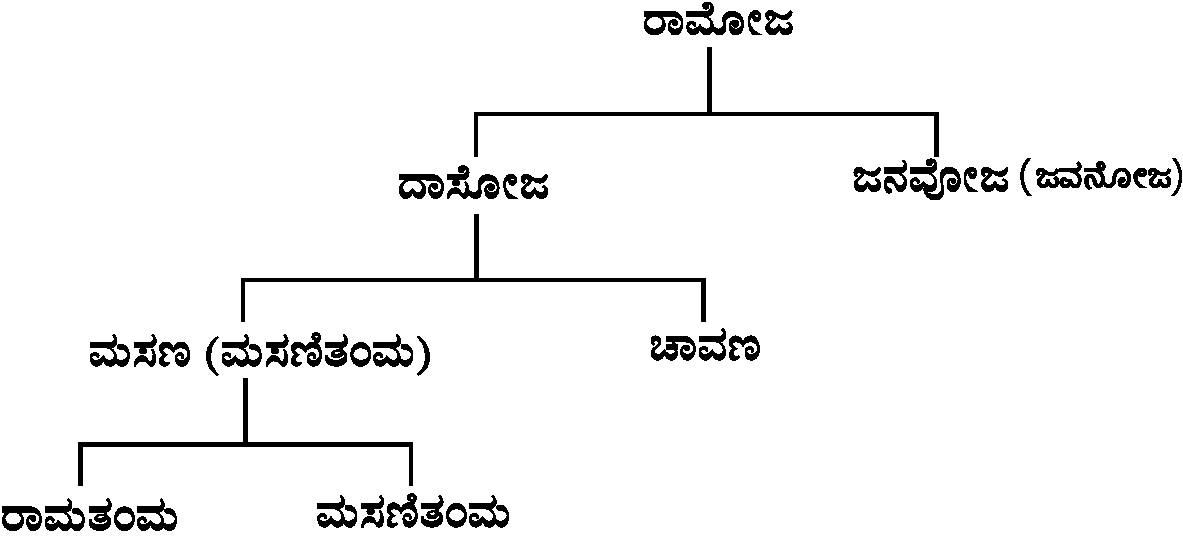
\includegraphics{"images/chap5/chap5fig3.jpeg"}
\end{figure}

“ತಮ್ಮ ಎಂಬ ಉಪನಾಮವು ಬೆಂಗಳೂರು, ಮಂಡ್ಯ, ಮೈಸೂರು ಮತ್ತು ಹಾಸನ ಜಿಲ್ಲೆಗಳಲ್ಲಿ ಪ್ರಚಲಿತವಾಗಿರುವುದ\-ರಿಂದ ಮಲ್ಲಿತಮ್ಮ ಮತ್ತು ಮಸಣಿತಮ್ಮರು ಜನ್ಮತಃ ಈ ಭಾಗಕ್ಕೆ ಸೇರಿದವರು” ಎಂದು ಚಿದಾನಂದಮೂರ್ತಿಯವರು ಅಭಿಪ್ರಾಯಪಟ್ಟಿದ್ದಾರೆ.\endnote{ ಚಿದಾನಂದಮೂರ್ತಿ ಡಾ॥ ಎಂ., ಸಂಶೋಧನಾ ತರಂಗ, ಭಾಗ 2, ಪುಟ 2} ಮೇಲೆ ಉಲ್ಲೇಖಿಸಿದಂತೆ ಇವರು ಮಳವಳ್ಳಿ ತಾಲ್ಲೂಕು ಗೌಡಗೆರೆಯಲ್ಲಿ ಭೂಮಿಯನ್ನು ಪಡೆದಿರುವುದು ಇದಕ್ಕೆ ಪುಷ್ಟಿ ನೀಡುತ್ತದೆ. ಮಂಡ್ಯ ಜಿಲ್ಲೆಯಲ್ಲಿ ತಮ್ಮಣ್ಣ, ಸಣ್ಣತಮ್ಮಣ್ಣ, ದೊಡ್ಡತಮ್ಮಣ್ಣ, ಎಂಬ ಹೆಸರುಗಳು ಹೆಚ್ಚಾಗಿ ಪ್ರಚಲಿತವಾಗಿರುವುದರಿಂದ ಈ ಅಭಿಪ್ರಾಯ ಒಪ್ಪತಕ್ಕದ್ದಾಗಿದೆ. ಮಲ್ಲಿತಮ್ಮ ಮಸಣಿತಮ್ಮ ಎಂಬ ಹೆಸರುಗಳನ್ನು ನೋಡಿದರೆ ಇವರು ಶೈವೋಪಾಸಕರೆಂದು ಹೇಳಬಹುದೆಂದು ಕುಮಾರಸ್ವಾಮಿ ಅಭಿಪ್ರಾಯಪಟ್ಟಿದ್ದಾರೆ.\endnote{ ಕುಮಾರಸ್ವಾಮಿ ಡಾ॥ ಕೆ.ಎಸ್​., ಪೂರ್ವೋಕ್ತ, ಪುಟ 144}

\textbf{ನಖರಾಚಾರಿ:} ಕಿಕ್ಕೇರಿಯ ಬ್ರಹ್ಮೇಶ್ವರ ದೇವಾಲಯದ ನಂದಿ ಮಂಟಪದ ತಳಪಾದಿಯ ಕಲ್ಲಿನ ಮೇಲೆ “ನಖರಾಚಾರಿ” ಎಂಬ ಬರಹವಿದೆ.\endnote{ ಎಕ 6 ಕೃಪೇ 30 ಕಿಕ್ಕೇರಿ 12ನೇ ಶ.} ಈ ಸುಂದರವಾದ ನಂದಿ ಮಂಟಪವನ್ನು ಅದರೊಳಗಿರುವ ಸುಂದರವಾದ ನಂದಿಯ ವಿಗ್ರಹವನ್ನು ನಖರಾಚಾರಿ ಎಂಬ ಶಿಲ್ಪಿ ನಿರ್ಮಿಸಿರಬಹುದೆಂದು ಊಹಿಸಬಹುದು. ಕಿಕ್ಕೇರಿಯ ಪಕ್ಕದಲ್ಲೇ ಇರುವ ಬೇಚಿರಾಕ್​ ಗ್ರಾಮ ಬದ್ರಿಹಾಳಿನ ಶಾಸನದಲ್ಲಿ “ಸಾಸನ ಸೂತ್ರಧಾರಿ ನಕರಾಚಾರಿ ಯಿ ಭೂಮಿಗೆ ಹುಟ್ಟಿದ (ಅ)ವನ ಮಗ ಬುಜಬಲಾಚಾರಿ” ಎಂದು ಹೇಳಿದೆ.\endnote{ ಎಕ 6 ಕೃಪೇ 22 ಬದ್ರೀಹಾಳ್​(ಬೇಚಿರಾಕ್​) 12ನೇ ಶ.} ಈತನೂ, ಕಿಕ್ಕೇರಿ ಶಾಸನೋಕ್ತ ನಕರಾಚಾರಿಯೂ ಅಭಿನ್ನರೆಂದು ಹೇಳಬಹುದು. ನಕರಾಚಾರಿಯ ಮಗ ಭುಜಬಲಾಚಾರಿ ಎಂದು ಹೇಳಬಹುದು.

\textbf{ದ್ರೋಹಘರಟ್ಟಾಚಾರಿ:} ಮಹಾಪ್ರಧಾನ ದಂಡನಾಯಕ ಗಂಗರಾಜನ ಮಗ ಬೊಪ್ಪದೇವನು ಕಟ್ಟಿಸಿದ ಕಂಬದಹಳ್ಳಿಯ ಶಾಂತಿನಾಥ ಬಸದಿಯನ್ನು \textbf{“ರೂವಾರಿ ದ್ರೋಹಘರಟ್ಟಾಚಾರಿ ಕನ್ನೆವಸದಿಯಂ ಮಾಡಿದ” }ನೆಂದು ತಿಳಿದುಬರುತ್ತದೆ.\endnote{ ಎಕ 7 ನಾಮಂ 32 ಕಂಬದಹಳ್ಳಿ} ಈ ಬಸದಿಯು ವಿಷ್ಣುವರ್ಧನನ ಕಾಲದಲ್ಲಿ ನಿರ್ಮಿತವಾಗಿದೆ. ದ್ರೋಹಘರಟ್ಟಾಚಾರಿ ಎಂಬುದು ರೂವಾರಿಯ ಬಿರುದಾಗಿದ್ದು ಇವನ ನಿಜ ಹೆಸರನೇನೋ ತಿಳಿಯದು.

\newpage

\textbf{ಮಲ್ಲಿತಮ್ಮ:} ಈತನು ಹೊಯ್ಸಳರ ಕಾಲದ ಪ್ರಸಿದ್ಧ ಶಿಲ್ಪಿ. ಇವನ ಜೀವನ ಸಾಧನೆಗಳನ್ನು ವಿದ್ವಾಂಸರು ಕಟ್ಟಿಕೊಟ್ಟಿದ್ದಾರೆ.\endnote{ ಕುಮಾರಸ್ವಾಮಿ ಡಾ॥ ಕೆ.ಎಸ್​., ಪೂರ್ವೋಕ್ತ, ಪುಟ 43-49} ಗೋವಿಂದನಹಳ್ಳಿಯ ಪಂಚಲಿಂಗೇಶ್ವರ ದೇವಾಲಯದ ಸುಂದರವಾದ ದ್ವಾರಪಾಲಕರುಗಳ ಪೀಠಗಳ ಮೇಲೆ \textbf{‘ರೂವಾರಿ ಮಾಲಿತಮ’, ‘ರೂವಾರಿ ಮಲಿತಂಮ’} ಎಂಬ ಶಿಲಾಲೇಖವಿದೆ.\endnote{ ಎಕ 6 ಕೃಪೇ 40 ಗೋವಿಂದನಹಳ್ಳಿ 13ನೇ ಶ.} ಮಲ್ಲಿತಮ್ಮನು ಕೇವಲ ದ್ವಾರಪಾಲಕರ ಮೂರ್ತಿಯ ಶಿಲ್ಪಿಯಾಗಿರದೇ, ಇಡೀ ದೇವಾಲಯದ ಪ್ರಧಾನ ಶಿಲ್ಪಿಯಾಗಿರಬಹುದೆಂದು ತೋರುತ್ತದೆ. ನುಗ್ಗೇಹಳ್ಳಿಯ ಲಕ್ಷ್ಮೀನರಸಿಂಹ ದೇವಾಲಯವನ್ನೂ ಇವನೇ ನಿರ್ಮಿಸಿರಬಹುದು.\endnote{ ಕುಮಾರಸ್ವಾಮಿ ಡಾ॥ ಕೆ.ಎಸ್​., ಪೂರ್ವೋಕ್ತ, ಪುಟ 44} ಗೋವಿಂದನಹಳ್ಳಿ ದೇವಾಲಯವೂ ಇದೇ ಕಾಲದಲ್ಲಿ ಇವನಿಂದ ರಚಿತವಾಗಿರಬಹುದು. ಮಲ್ಲಿತಮ್ಮ ಮತ್ತು ಮಸಣಿತಮ್ಮ ಇಬ್ಬರೂ ಸೋಮನಾಥಪುರ ದೇವಾಲಯದ ಪ್ರಮುಖ ಶಿಲ್ಪಿಗಳಾಗಿ ಅನೇಕ ಪ್ರಮುಖ ವಿಗ್ರಹಗಳನ್ನು ಕಡೆದಿರುವುದು ಅಲ್ಲಿನ ಶಾಸನಗಳಿಂದ ತಿಳಿದುಬರುತ್ತದೆ.\endnote{ ಎಕ 5 ತೀನಪು 93 ಸೋಮನಾಥಪುರ 1268}

\textbf{ಪಟ್ಟಣೋಜನ ಮಗ ಚಿಕಬಾಚೆಯ:} ಕನ್ನಂಬಾಡಿಯಲ್ಲಿರುವ ಹೊಯ್ಸಳರ ಕಾಲದ ಗೋಪಾಲಕೃಷ್ಣ ದೇವಾಲಯದ ಮುಖ ಮಂಟಪದ ಮೇಲೆ “ಪಟ್ಟಣೋಜನ ಮಗ ಚಿಕಬಾಚೆಯನ ಅಂಕಣ” ಎಂಬ ಹೆಸರಿದ್ದು, ಈ ಮುಖಮಂಟಪವನ್ನು ಇವನೇ ರಚಿಸಿರುವಂತೆ ತೋರುತ್ತದೆ.\endnote{ ಎಕ 6 ಪಾಂಪು 32 ಕನ್ನಂಬಾಡಿ 13ನೇ ಶ.} ಇವನು ಈ ದೇವಾಲಯದ ಶಿಲ್ಪಿಗಳಲ್ಲಿ ಒಬ್ಬನಾಗಿರಬಹುದು.

\textbf{ಪಂಚಾಳದವರು(ಪಾಂಚಾಳದವರು):} ಪಂಚಾಳ ಅಥವಾ ಪಾಂಚಾಳದವರಲ್ಲಿ ಶಿಲ್ಪಿಗಳು, ರೂವಾರಿಗಳು,\break ಅಕ್ಕಸಾಲಿಗರು, ಕಮ್ಮಾರರು ಎಲ್ಲರೂ ಸೇರಿದ್ದಾರೆಂದು ಹೇಳಬಹುದು. ಶಾಸನಗಳಲ್ಲಿ ಪಂಚಾಳರು ಊರಿನ ಪಂಚರಲ್ಲಿ ಅಥವಾ ಅಧಿಕಾರವರ್ಗ\-ದವರಲ್ಲಿ ಒಬ್ಬರಾಗಿರುವಂತೆ ತೋರುತ್ತದೆ. “ಒಬ್ಬನೇ ವ್ಯಕ್ತಿಯು ಮರಗೆಲಸ, ಕಬ್ಬಿಣದ ಕೆಲಸ, ಚಿನ್ನದ ಕೆಲಸ, ಲೋಹದ(ಕಂಚು)ಕೆಲಸ ಮತ್ತು ಕಲ್ಲಿನ ಕೆಲಸಾದಿಗಳಲ್ಲಿ ಬಲ್ಲಿದನಾಗಿರುತ್ತಿದ್ದನು. ಇದರಿಂದ ಈ ವೃತ್ತಿಗಳು ಪರಸ್ಪರ ಪೂರಕ ಹಾಗೂ ಪೋಷಕವಾಗಿದ್ದು ಒಂದೇ ಸಾಂಸ್ಕೃತಿಕ ಮೂಲದಿಂದ ಬಂದವುಗಳಾಗಿದ್ದಿರಬೇಕೆಂದು ತಿಳಿಯುತ್ತದೆ” ಮತ್ತು “ಈ ಕಸುಬಿನವರನ್ನು ಒಂದೇ ಎಂದು ಪರಿಗಣಿಸಿ ಇವರನ್ನು ಪಂಚಕಾರುಕರು ಎಂದು ಕರೆದು ‘ಪಂಚಕಾರುಕ’ ಎಂಬ ತೆರಿಗೆಯನ್ನು ವಿಧಿಸಲಾಗುತ್ತಿತ್ತು” ಎಂದೂ ತಿಳಿದುಬರುತ್ತದೆ.\endnote{ ಕುಮಾರಸ್ವಾಮಿ ಡಾ. ಎಸ್​.ಕೆ., ಪೂರ್ವೋಕ್ತ, ಪುಟ 128} ಕೃಷ್ಣರಾಜಪೇಟೆ ತಾಲ್ಲೂಕು ಭೈರಾಪುರದ ಒಂದು ಕ್ರಯ ಶಾಸನದಲ್ಲಿ \textbf{“ಗದ್ದೆಯನು ಸರ್ವಮಾನ್ಯವಾಗಿ ಸಲಿಸಿ ಕೊಡುಉದಕೆ ಹೊಣೆಕಾರರು ಭಯಿರಾಪುರದ ಒಜಾಯಿತ ಲಖೋಜ, ಅಕಸಾಲೆ ಸಭೆಯೋಜ, ಅಕಸಾಲೆ ಮಂಚಿ ಹಿರಿಯ ಕಾಮೋಜಗಳು ಒಳಗಾದ ಪಂಚಾಳದವರು ಹೊಣೆ”} ಎಂದು ಹೇಳಿದೆ.\endnote{ ಎಕ 6 ಕೃಪೇ 95 ಭೈರಾಪುರ 1312}\break \textbf{ “ಮಾಣಿಕೋಜ, ದೇವೋಜ, ಬೆಳಕವಾಡಿಯ ಬೊಂಮೋಜನೊಳಗಾದ ಪಾಂಚಾಳದವರು”} ಗವುಡು ಪ್ರಜೆಗಳು, ಪಟ್ಟಣಸ್ವಾಮಿ\-ಗಳು ಇವರ ಜೊತೆ ಸೇರಿ ಗ್ರಾಮವನ್ನು ದತ್ತಿಯಾಗಿ ಬಿಟ್ಟರೆಂದು ದಾಸನದೊಡ್ಡಿ ಶಾಸನದಲ್ಲಿ ಹೇಳಿದೆ.\endnote{ ಎಕ 7 ಮವ 90 ದಾಸನದೊಡ್ಡಿ 1463}\textbf{ “ಆಚೋಜ, ಲಕೋಜ”} ಇವರು ಮಲ್ಲಿಕಾರ್ಜುನಪುರ ಅಗ್ರಹಾರದಲ್ಲಿ ಭೂಮಿಯ ಕ್ರಯ ಹಾಗೂ ತೆರಿಗೆ ಪಾವತಿಯ ವಿಚಾರದಲ್ಲಿ ಸಾಕ್ಷಿಗಳಾಗಿದ್ದಾರೆ.\endnote{ ಎಕ 7 ಮಂ 60 ಗುತ್ತಲು 1316} ಸ್ಥಳ ಪಾಂಚಾಲದ ಹಿರಿಯರಾದ ತಿರುಮಲೆ ಕೃಷ್ಣಯ್ಯನವರ ಮೊಮ್ಮಕ್ಕಳು ಲಕ್ಷ್ಮೀದೇವಿಗೆ ವಜ್ರದ ಅಂಗಿ, ಪೀಠ, ಪ್ರಭಾವಳಿಗಳನ್ನು ಮಾಡಿಸಿಕೊಟ್ಟರೆಂದು ದೇವರಹಳ್ಳಿ ಶಾಸನದಲ್ಲಿ ಹೇಳಿದೆ. ಇವರು ಸ್ಥಳದಲ್ಲೇ ನೆಲೆಸಿದ್ದು ಅಕ್ಕಸಾಲಿಕೆಯನ್ನು ಮಾಡುತ್ತಿದ್ದರೆಂದು ಹೇಳಬಹುದು.\endnote{ ಎಕ 7 ನಾಮಂ 148 ದೇವರಹಳ್ಳಿ 19ನೇ ಶ.}

\textbf{ರೂವಾರಿಗಳು:} ಶಿಲ್ಪಸಹಿತವಾದ ಮತ್ತು ಶಿಲ್ಪ ರಹಿತವಾದ ಶಾಸನಗಳು, ಶಿಲ್ಪ ಮತ್ತು ಬರಹ ಎರಡೂ ಇರುವ, ಹಾಗೂ ಕೇವಲ ಶಿಲ್ಪವಿರುವ ಸ್ಮಾರಕ ಶಿಲೆಗಳನ್ನು, ಕಲ್ಲಿನ ಮೇಲೆ ಬಿಡಿಸುತ್ತಿದ್ದವರು ಅಥವಾ ಕೆತ್ತುತ್ತಿದ್ದವರನ್ನು ಶಾಸನ ರೂವಾರಿಗಳೆಂದು ಕರೆಯಬಹುದು. ಇವರಲ್ಲಿ ಆಚಾರಿಗಳು, ಅಕ್ಕಸಾಲೆಗಳು, ಓಜರು ಎಲ್ಲರೂ ಸೇರಿದ್ದಾರೆ. ಶಾಸನಕ್ಕೆ ಸೂಕ್ತವಾದ ಕಲ್ಲನ್ನು ಸಿದ್ಧಪಡಿಸಿ ಕೊಡುವುದು, ಆನಂತರ ಅದರ ಮೇಲೆ ಶಿಲ್ಪವನ್ನು ಮತ್ತು ಶಾಸನ ಲೇಖಕನು ಬರೆದ ಬರಹವನ್ನು ಕಂಡರಿಸುವ ಕೆಲಸವನ್ನು ‘ರೂಹಾರಿಗಳು ಅಥವಾ ರೂವಾರಿಗಳು’ ಮಾಡುತ್ತಿದ್ದರು. ಕಡ್ಲವಾಗಿಲಿನ ಶಾಸನಸ್ತ ದೊಡ್ಡ ವೀರಗಲ್ಲಿನಲ್ಲಿ ‘ಇ ಕಲ್ಲಂ ರೂಹಾರ ಮಾಡಿದನು ಪುರದಾಚಾರಿಯ ಮಗ ಮಂಡಳಿಕಾಚಾರಿ’ ಎಂದು ಹೇಳಿದೆ.\endnote{ ಎಕ 7 ಮ 120 ಕಡ್ಲವಾಗಿಲು 1192} ಇನ್ನೊಂದು ದೊಡ್ಡ ವೀರಗಲ್ಲಿನಲ್ಲೂ ಇವನ ಹೆಸರಿದ್ದು ಅದು ತ್ರುಟಿತವಾಗಿದೆ\textbf{\endnote{ ಎಕ 7 ಮ 118 ಕಡ್ಲವಾಗಿಲು 1192}}. ಇಲ್ಲಿರುವ ಅನೇಕ ಶಿಲ್ಪಸಹಿತವಾದ ದೊಡ್ಡ ದೊಡ್ಡ ವೀರಗಲ್ಲುಗಳನ್ನು ಇವನೇ ನಿರ್ಮಿಸಿರಬಹುದು. ಇವನೊಬ್ಬ ದೊಡ್ಡ ರೂವಾರಿಯಾಗಿರಬಹುದೆಂದು ಇದರಿಂದ ತಿಳಿದುಬರುತ್ತದೆ. ರೂಹಾರ(ವ) ಎಂಬ ಕ್ರಿಯಾಪದವೇ ರೂವಾರಿ ಎಂಬ ನಾಮ ಪದದ ಮೂಲವಾಗಿದೆ. ರೂಹು ಎಂದರೆ ರೂಪು. ಕಲ್ಲಿನ ಮೇಲೆ ಶಿಲ್ಪವನ್ನು, ಅಕ್ಷರಗಳನ್ನೂ ಕೆತ್ತಿ ಅದಕ್ಕೆ ಒಂದು ರೂಪು ಕೊಡುವವನೇ ರೂಹಾರಿ. ಈ ಕ್ರಿಯೆಯೇ ರೂಹಾರ. ರೂವಾರಿಗಳೆಂದರೂ ಶಿಲ್ಪಿಗಳೇ. ಕೆಲವೊಮ್ಮೆ ದೇವಾಲಯ ನಿರ್ಮಾಣ ಮತ್ತು ಶಾಸನ ಕೆತ್ತನೆ ಎರಡನ್ನೂ ಒಬ್ಬರೇ ಮಾಡಿದ ಉದಾಹರಣೆಗಳಿವೆ. ಪಂಡಿತೋಜನು \textbf{‘ದೇಗಳಂ ಮಾಡಿ ಸಾಸನಂ ಬರೆದ’} ಎಂದು ಹೇಳಿದೆ. ರೂವಾರಿ ಮಲ್ಲಿತಮ್ಮನು ಸಾಲಗಾಮೆಯ ಶಾಸನವನ್ನು ಕೆತ್ತಿದ್ದಾನೆ.\endnote{ ಕುಮಾರಸ್ವಾಮಿ ಡಾ॥ ಕೆ.ಎಸ್​., ಪೂರ್ವೋಕ್ತ, ಪುಟ 44} ಜಿಲ್ಲೆಯ ಶಾಸನಗಳಲ್ಲಿ ಇಂತಹ ಅನೇಕ ರೂವಾರಿಗಳು ಕಂಡುಬರುತ್ತಾರೆ. ಇವರು ದೇವಾಲಯವನ್ನು ನಿರ್ಮಿಸಿದ್ದಾರೋ ಇಲ್ಲವೋ ತಿಳಿಯದು. ಆದರೆ ಶಾಸನಗಳನ್ನು ಕಂಡರಿಸಿರುವುದು ಖಚಿತ.

\vskip 3pt

ಜಿಲ್ಲೆಯಲ್ಲಿರುವ ಗಂಗರ ಕಾಲದ ತಾಮ್ರ ಅಥವಾ ಶಿಲಾಶಾಸನಗಳಲ್ಲಿ ಶಾಸನಗಳನ್ನು ಕೊರೆದ ರೂವಾರಿಗಳ ಹೆಸರು ಹೆಚ್ಚಾಗಿ ಕಂಡು ಬರುವುದಿಲ್ಲ. ದೇವರಹಳ್ಳಿಯ ಶ‍್ರೀಪುರುಷನ ತಾಮ್ರ ಶಾಸನದಲ್ಲಿ \textbf{“ಸರ್ವ್ವಕಲಾಧಾರಭೂತ ಚಿತ್ರಕಲಾಭಿಜ್ಞೇನ ವಿಶ್ವಕರ್ಮ್ಮಾಚಾರ್ಯ್ಯೇಣೇದಂ ಶಾಸನಮ್ ಲಿಖಿತಮ್ ಚತುಷ್ಕಣ್ಡುಗ ಬ್ರೀಹಿ ಬೀಜಾವಾಪಮಾತ್ರಂ ದ್ವಿಕಣ್ಡುಗ ಕಙ್ಗು ಕ್ಷೇತ್ರಂ”,}\endnote{ ಎಕ 7 ನಾಮಂ 149 ದೇವರಹಳ್ಳಿ 776-77}ಎಂದು ಹೇಳಿದೆ. ಈ ತಾಮ್ರ ಶಾಸನವನ್ನು ವಿಶ್ವಕರ್ಮಾಚಾರ್ಯನು ಕಂಡರಿಸಿದ್ದು, ಅವನಿಗೆ ಗದ್ದೆ ಮತ್ತು ಅಡಕೆ ತೋಟವನ್ನು ಕೊಡುಗೆಯಾಗಿ ನೀಡಿದೆ. ವಿಶ್ವಕರ್ಮ ಎಂಬುದು ಶಾಸನ ಇಲಾಖೆಯ ಅಧಿಕಾರಿ ಅಥವಾ ಮುಖ್ಯಸ್ಥನ ಹುದ್ದೆಯಾಗಿದ್ದು ಅವನ ನಿಜನಾಮವಾಗಿರುವುದಿಲ್ಲವೆಂದು ಹೇಳಬಹುದು.\endnote{ ಕುಮಾರಸ್ವಾಮಿ, ಡಾ॥ಎಸ್​.ಕೆ., ಪೂರ್ವೋಕ್ತ, ಪುಟ 14-15} ಆರಣಿಯ ಶಾಸನವನ್ನು “ಅಡೆಪಯ್ಯಂ ಮಾಡಿಸಿದ”,\endnote{ ಎಕ 7 ನಾಮಂ 99 ಆರಣಿ 972} ಎಂದು ಹೇಳಿದೆ. ಬಹುಶಃ ಈತನು ಶಾಸನದ ರೂವಾರಿಯಾಗಿರಬಹುದು. ಅಡೆಕಲ್ಲುವಣ ಎಂಬ ಒಂದು ತೆರಿಗೆ ಇದ್ದಿತೆಂದೂ, ಅಡೆಕಲ್ಲು ಎಂದರೆ ಕಮ್ಮಾರರು ಉಪಯೋಗಿಸುವ ಅಡಿಗಲ್ಲು ಎಂದೂ ತಿಳಿದುಬರುತ್ತದೆ.\endnote{ ಕುಮಾರಸ್ವಾಮಿ ಡಾ॥ ಎಸ್​.ಕೆ., ಪೂರ್ವೋಕ್ತ, ಪುಟ 110-11} ಇದೇ ಅಡೆಪಯ್ಯ ಹೆಸರಿನ ನಿಷ್ಪತ್ತಿಯ ಮೂಲವಿರಬಹುದು. ವಿಜಯನಗರ ಕಾಲದಲ್ಲಿ ಒಡೆಯಪ್ಪಯ್ಯ ವಿಶ್ವನಾಥನೆಂಬುವವನು ವಿಶ್ವಕರ್ಮಕುಲದ ಜಗದ್ಗುರುವಾಗಿದ್ದನೆಂದು ತಿಳಿದುಬರುತ್ತದೆ.\endnote{ ಕುಮಾರಸ್ವಾಮಿ, ಡಾ॥ ಎಸ್​.ಕೆ., ಪೂರ್ವೋಕ್ತ, ಪುಟ 139} ಇದು ಅಡೆಯಪ್ಪಯ್ಯ ಎಂದಿದ್ದಿರಬಹುದು.

\vskip 3pt

\textbf{ಕಲ್ಲುಕುಟಿಗ:} ಶಾಸನಗಳನ್ನು ಕಂಡರಿಸಿರುವ ಕೆಲವರು ಕಲ್ಲುಕುಟಿಗ ಎಂಬ ವೃತ್ತಿವಿಶೇಷಣದಿಂದಲೇ ತಮ್ಮನ್ನು ಗುರುತಿಸಿಕೊಂಡಿದ್ದಾರೆ. ಕಲ್ಕುಟಿಕರು ತಮ್ಮನ್ನು ರೂವಾರಿಗಳೆಂದೂ ಕರೆದುಕೊಂಡಿದ್ದಾರೆ. ‘ಇ ಕಲ್ಲ ಪೊಯ್ದ ಕಲ್ಕುಟಿಗ ಲಖೋಜ’,\endnote{ ಎಕ 6 ಶ‍್ರೀಪ 113 ಅರಕೆರೆ 1108} “ರೂವಾರಿ ಕಲ್ಕುಟಿಕ ಕೇತೋಜ ಖಂಡಿಸಿದ॥ ಕವಣಿಕೆ 57 ವ. ನು(ಪ)ಡದ”,\endnote{ ಎಕ 7 ನಾಮಂ 98 ಮುದಿಗೆರೆ 1139} “ಬಿನಕೋಜನ ಮಗ ಕಲ್ಲುಕುಟಿಗ ದೇವರಸ ದೀಪಮಾಲೆಯ ಕಂಬಗೈದು ನಿಲಿಸಿದಕ್ಕೆ ಸರ್ವಮಾನ್ಯವಾಗಿ ಪಾಲಿಸಿದ ಕೊಡಗಿಯ ಗದ್ದೆ”\endnote{ ಎಕ 7 ಮವ 73 ಮಾರೇಹಳ್ಳಿ 15-16ನೇ ಶ.}, ‘ಕಲ್ಲುಕುಟಿಗ ದೇವರಸ ಕಂಡ(ರಿಸಿದ\textbf{)}’\endnote{ ಎಕ 7 ಮವ 76 ಮಾರೇಹಳ್ಳಿ 15-16ನೇ ಶ.} ಎಂಬ ಉಲ್ಲೇಖಗಳಲ್ಲಿ ಕಲ್ಲುಕುಟಿಗ ಎಂಬ ವಿಶೇಷಣಗಳನ್ನು ಬಳಸಲಾಗಿದೆ. ಈ ಶಾಸನಗಳಲ್ಲಿ ಕಲ್ಲು ಕುಟಿಕರು ತಮ್ಮ ಕೆಲಸಕ್ಕೆ ಪಡೆದ ಪ್ರತಿಫಲವನ್ನು ನಮೂದಿಸಿರುವುದನ್ನು ಗುರುತಿಸಬಹುದು.

\vskip 3pt

\textbf{ಓಜ/ಓವಜರು:} ಶಾಸನದ ರೂವಾರಿಗಳು ಹೆಚ್ಚಾಗಿ ತಮ್ಮನ್ನು ಓಜ/ಓವಜ ಎಂಬ ಹೆಸರಿನಿಂದಲೇ ಗುರುತಿಸಿ\-ಕೊಂಡಿದ್ದಾರೆ. ‘ಕಾಮೋಜವೋಜ (ಕೊ)ರೆದ ಸಾಸನ’,\endnote{ ಎಕ 6 ಕೃಪೇ 73 ಹಿರಿಕಳಲೆ 12ನೇ ಶ.} ‘ರೂವಾರಿ ಬಮೋಜನ ಮಗಂ.ಹ ಪುರದಾಚಾರಿ ಕಂಡರಿಸಿದ’,\endnote{ ಎಕ 7 ನಾಮಂ 17 ಪುರದಕಟ್ಟೆ 1139}\- \textbf{‘ಶ‍್ರೀಮತು }ಮಾಣಿಕ್ಯವೊಳಲ ಮೂಲಸ್ಥ ಚನ್ದಕಕೋಜನ ಸುಪುತ್ರಂ ಪರವಾದಿ ಮಲ್ಲೋಜಂ ಗೆಯ್ದಂ ಶಾಸನಮಂ’, ‘ಶ‍್ರೀ ಬೆಳ್ಗೊಳದ ಹೊಯ್ಸಳಾಚಾರಿಯ ತಮ್ಮಂ ವೈಚೋಜಂಗೆಯ್ದ ಸಾಸನ’,\endnote{ ಎಕ 6 ಕೃಪೇ 22 ಬದ್ರೀಹಾಳ್​(ಬೇಚಿರಾಕ್​) 12ನೇ ಶ.}\textbf{‘ಇ ಸ್ಯಾಸನವ ಬರದತ ರಾಮೋಜನ ಜವನೋಜ’,\endnote{ ಎಕ 6 ಕೃಪೇ 88 ಸಿಂಧಘಟ್ಟ 1179}}‘ಇ ಸಾಸನವ ಹೊಇದ ಜವನೋಜ’,\endnote{ ಎಕ 6 ಕೃಪೇ 90 ಸಿಂಧಘಟ್ಟ 1299} ಎಂದು ಜಿಲ್ಲೆಯ ಶಾಸನಗಳಲ್ಲಿ ಹೇಳಿದೆ. ನಾಗೊಡೆಯನ ವೀರಗಲ್ಲನ್ನು ‘ಕಂಚಿಗೋಜನ ಮಗ ಬಳಗೋಜ’ ಮಾಡಿದ್ದಾನೆ.\endnote{ ಎಕ 7 ಮವ 39 ಹುಲ್ಲೇಗಾಲ 12-13ನೇ ಶ.} ‘ಸೀತೋಜನ ಮಗ ಅರುಳಿಯೋಜಂಗೆ ದುಡೋಜನು’ ವೀರಗಲ್ಲನ್ನು ನಿಲ್ಲಿಸಿದ್ದಾನೆ.\endnote{ ಎಕ 7 ಮಂ 6 ಮಂಡ್ಯ 1204} ‘ಏಚೋಜನ ಮಗ ಸಿದೋಜನು’ ಚಿಕಮಾಯಿನಾಯಕನ ‘ಬೀರಗಲು’ ನಿಲ್ಲಿಸಿದ್ದಾನೆ.\endnote{ ಎಕ 7 ನಾಮಂ 109 ಚುಂಚನಹಳ್ಳಿ 13ನೇ ಶ.} ‘ಬೀರಕಲನು ನಂಜೆಯ ಕೇತೋಜರು ಆಕಿ ಮಾಡಿದನು’,\endnote{ ಎಕ 7 ನಾಮಂ 106 ಹೊನ್ನೇನಹಳ್ಳಿ 1180} ‘ದಾಯೋಜನ ಮಗ ದಾಯೋಜನು ಹುಯಿಸಿದ ವೀರಗಲ್ಲು’,\endnote{ ಎಕ 7 ಮ 119 ಕಡ್ಲವಾಗಿಲು 13ನೇ ಶ.} ಎಂದು ಹೇಳಿದ್ದು, ಇದರಿಂದ ತಂದೆ ಮತ್ತು ಮಕ್ಕಳು ಒಂದೇ ಹೆಸರನ್ನು ಇಟ್ಟುಕೊಳ್ಳುತ್ತಿದ್ದು ತಿಳಿದುಬರುತ್ತದೆ. \textbf{ಅಗ್ರಹಾರ\-ಬಾಚಹಳ್ಳಿಯ ವೀರಗಲ್ಲಿನ ಮೇಲೆ ‘ಬಲೋಜನು ಕೂತೋಜನು ನಿಲಿಸಿದ ವೀರಸಾಸನ’}\endnote{ ಎಕ 6 ಕೃಪೇ 78 ಅಗ್ರಹಾರಬಾಚಹಳ್ಳಿ 1224} ಎಂದು ಹೇಳಿದ್ದು, ಇವರಿಬ್ಬರೂ ಈ ಊರಿನ ಪ್ರಸಿದ್ದ ಗರುಡ ವೀರಸ್ಥಂಭಗಳನ್ನು, ಶಾಸನಗಳನ್ನು ಕಡೆದಿರುವ ಸಾಧ್ಯತೆ ಇದೆ. ‘ಮರಕೋಜನು’ ಹುಸ್ಕೂರಿನ ಬಸದಿಯನ್ನು ನಿರ್ಮಿಸಿರಬಹುದು.\endnote{ ಎಕ 7 ಮವ 31 ಹುಸ್ಕೂರು 1313} ‘ಬಂಮೋ(ಜ)ನ ಕಂಡರ(ಣೆ)’\endnote{ ಎಕ 7 ಮವ 44 ನಡಗಲ್​ಪುರ 1510}, ‘ನಂಬಿಯೋಜನ ಬರಹ’\endnote{ ಎಕ 7 ಮವ 32 ಹುಸ್ಕೂರು 1440} ‘ಸಸನ ಕಲ ಹುದವ ಮಾಯಿವೋಜನ ಮಗ ಕೇತಣ’\endnote{ ಎಕ 7 ಮವ 43 ಬಸವನಪುರ 1513}, ಇವರು ಜಿಲ್ಲೆಯ ಶಾಸನಗಳಲ್ಲಿ ಕಂಡು ಬರುವ ಶಾಸನದ ಕಲ್ಲನ್ನು ನಿರ್ಮಿಸಿ, ಕಂಡರಣೆ ಮಾಡಿದ ಓವಜರು.

\vskip 3pt

\textbf{ಕೆರಗೆ ತೂಬನ್ನಿಕ್ಕಿದ, ಕೆರೆಯನ್ನು ಕಟ್ಟಿಸಿದ ಓಜರು: } ಕೆರೆ ಮತ್ತು ತೂಬುಗಳ ನಿರ್ಮಾಣದಲ್ಲಿಯೂ ಈ ಶಿಲ್ಪಿಗಳು ಪ್ರಮುಖ ಪಾತ್ರ ವಹಿಸುತ್ತಿದ್ದರೆಂದು ತಿಳಿದುಬರುತ್ತದೆ. ಬೊಯ್ಸಿ ಕಟ್ಟೆಗೆ \textbf{“ತೂಂಬನಿರಿಸಿದ ಮಾೞಿಯಕ್ಕಾಚಾರಿಗೆ 10 ಕಣ್ಡುಗ ಮಣ್ನು”} ದತ್ತಿ ಬಿಡಲಾಗಿದೆ.\endnote{ ಎಕ 7 ಮಂ 67 ಬೇಲೂರು 1022} ‘ಕಾಜನ ಮಗ ಕೋಲೋಜ’ ಕಟ್ಟಿಸಿದ ಕೆರೆಗೆ ಕಿರುಗುಂದೂರ ಗವುಡುಗಳು ದತ್ತಿ ಬಿಟ್ಟ ವಿಚಾರ ಶಾಸನೋಕ್ತವಾಗಿದೆ.\endnote{ ಎಕ 7 ಮಂ 87 ಕಿರಗಂದೂರು 1456} ಬಹುಶಃ ಈ ಕೆರೆಯ ಶಿಲ್ಪಿ ಅಥವಾ ತಂತ್ರಜ್ಞ ಇವನೇ ಆಗಿರಬಹುದು. ಜಿಲ್ಲೆಯ ಶಾಸನಗಳಲ್ಲಿ ಈ ರೂವಾರಿಗಳ ಬಗ್ಗೆ ಸಾಕಷ್ಟು ಮಾಹಿತಿಗಳು ದೊರೆಯುತ್ತವೆ.

ಓಜರು ಕೆರೆಯನ್ನು ಕಟ್ಟಿಸಿದ ಉದಾಹರಣೆಗಳಿವೆ. ‘ಕಿರಗುಂದೂರ ಗುಳಯನ ಮಗ ಲಕ್ಕಯ್ಯ, ಮಂಚಯ್ಯನ ಮಗ ಆದಿಮಂಡಳ, ಕಾಜನ ಮಗ ಕೋಲೋಜ’ ಇವರೂ ಮೂರೂ ಸೇರಿ ಕೆರೆ ಕಟ್ಟೆಯನ್ನು ಕಟ್ಟಿಸುತ್ತಾರೆ.\endnote{ ಎಕ 7 ಮಂ 87 ಕಿರುಗಂದೂರು 1456} ಬಹುಶಃ ಕೋಲೋಜನು ಈ ಕೆರೆಯ ಶಿಲ್ಪಿಯಾಗಿರಬಹುದು. ಓಜರು ಕಲ್ಲಿನ ಗಾಣವನ್ನೂ ಕೂಡಾ ಮಾಡುತ್ತಿದ್ದರು. ಜಿಲ್ಲೆಯ ಅನೇಕ ದೇವಾಲಯದ ಮುಂದೆ ಆ ಗಾಣಗಳೂ ಈಗಲೂ ನಿಂತಿವೆ. ಹಾದರವಾಗಿಲಿನಲ್ಲಿ ತೆಳ್ಳರ ಕುಲದ ಚಾಮಗಾಮುಂಡನು ತಿಪ್ಪೂರು ತೀರ್ಥದಲ್ಲಿ ಮಾಡಿಸಿದ ಗಾಣವನ್ನು \textbf{‘ಉಮೆಯನೊಡೆಯಂ ಪಂಡಿತೋಜನ ಹಸ್ತಕೌಸಲ್ಯಂ},\endnote{ ಎಕ 7 ಮ 106 ಹಾಗಲಹಳ್ಳಿ 1698} ಎಂದು ಹೇಳಿದೆ.

\textbf{ಆಚಾರಿ:} ಕೆಲವು ಶಾಸನ ರೂವಾರಿಗಳು ಆಚಾರಿ ಎಂಬ ವೃತ್ತಿ ವಿಶೇಷಣದಿಂದ ತಮ್ಮನ್ನು ಗುರುತಿಸಿಕೊಂಡಿದ್ದಾರೆ. ಆದರೂ ಇವರು ಓಜ ಎಂಬುದನ್ನೂ ತಮ್ಮ ಹೆಸರಿನ ಅಂತ್ಯದಲ್ಲಿ ಸೇರಿಸಿಕೊಂಡಿದ್ದಾರೆ. ಮಂಡ್ಯ ತಾಲ್ಲೂಕು ಹಂಪಾಪುರದ ವೀರಗಲ್ಲು ಶಾಸನವು ಬಹಳ ಕುತೂಹಲಕರವಾಗಿದೆ.\endnote{ ಎಕ 7 ಮಂ 23 ಹಂಪಾಪುರ 1221} ಇಮ್ಮಡಿ ಬಲ್ಲಾಳನ ಕಾಲದಲ್ಲಿ ರಂಗಗವುಡನು ಕಾದಿ ಮಡಿದಾಗ ಅವನಿಗೆ ವೀರಗಲ್ಲನ್ನು ಹಾಕಿಸಲಾಗಿರುತ್ತದೆ. ಈ ವೀರಗಲ್ಲನ್ನು ಆಚಾರಿ ಅಳಿಬನು ಮಾಡಿರುತ್ತಾನೆ. ಸುಮಾರು ವರ್ಷಗಳು ಕಳೆದ ನಂತರ ಈ ವೀರಗಲ್ಲು ಸವೆದಿರಲು, ರಂಗಗವುಡನ ಮಗ ಚಿಕ್ಕಗವುಡನು ಈ ವೀರಗಲ್ಲನ್ನು ತಿದ್ದಿಸಿ ಅಂದರೆ ಮತ್ತೆ ಕೆತ್ತಿಸಿ ಅದಕ್ಕೆ ಮೇಲು ಮುಚ್ಚಳವನ್ನು ಹಾಕಿಸುತ್ತಾನೆ. ಬಹುಶಃ ವೀರರಗುಡಿಯನ್ನು ಕಟ್ಟಿಸುತ್ತಾನೆ. ಈ ವೀರಗಲ್ಲು ಶಾಸನವನ್ನು ಹಿಂದೆ ಮಾಡಿದ್ದ ಆಚಾರಿ ಅಳಿಬನ ಮಗ ಮಲ್ಲಿಕಾರ್ಜುನ ಅಳಿಬ ಮತ್ತು ಮಂಚೋಜ ಇಬ್ಬರೂ ತಿದ್ದಿ ಕೊಡುತ್ತಾರೆ. ಅವರು ತಿದ್ದಿದಂತೆ ಆಚಾರಿ ಅಕಸಾಲೆ ಬಂದಿಯೋಜನ ಮಗ ಮಾಮಾರಿಯ ಅಂಚಿತಮಂನು ರೂವಾರಿಸುತ್ತಾನೆ. ಈ ವೀರಗಲ್ಲನ್ನು ಹೊಸದಾಗಿ ಮಾಡಿದ್ದಕ್ಕೆ ಮಾಮರಿಯ ಅಂಚಿತಮಂನಿಗೆ 6 ಗದ್ಯಾಣವನ್ನು, ತಿದ್ದಿಕೊಟ್ಟ ಮಲ್ಲಿಕಾರ್ಜುನ ಅಳಿಬ ಮತ್ತು ಮಂಚೋಜ ಇವರಿಬ್ಬರಿಗೂ ತಲಾ 6 ಗದ್ಯಾಣವನ್ನೂ ನೀಡಲಾಗುತ್ತದೆ. ಆಚಾರಿ, ಅಕಸಾಲೆ ಎಂಬ ಪದಗಳು ಒಟ್ಟಾಗಿ ಬಳಕೆಯಾಗಿವೆ. ಈ ವೃತ್ತಿಗಳಲ್ಲಿ ಅಲ್ಪ ಸ್ವಲ್ಪ ವ್ಯತ್ಯಾಸ ಇರಬಹುದು.

\textbf{ “ಪತ್ರಸಾಸನವ ನೋಡಿ ಬರದ ಆಚಾರಿ ಮಸಣೋಜ}”\endnote{ ಎಕ 7 ಮಂ 56 ಹೊಸಬೂದನೂರು 1276}, ಎಂದು ಹೊಸಬೂದನೂರು ಶಾಸನದಲ್ಲಿ ಹೇಳಿದ್ದು, ಮೊದಲು ಶಾಸನವನ್ನು ತಾಳ ಪತ್ರದ ಮೇಲೆ ಅಥವಾ ಬಟ್ಟೆಯ ಮೇಲೆ ಬರೆಯುತ್ತಿದ್ದು ಅದನ್ನು ನೋಡಿಕೊಂಡು ಕಲ್ಲಿನ ಮೇಲೆ ಬರೆದು ಅದನ್ನು ಕೆತ್ತುತ್ತಿದ್ದರೆಂಬುದು ಇದರಿಂದ ಖಚಿತವಾಗಿ ತಿಳಿದುಬರುತ್ತದೆ. \textbf{‘ತಲಕಾಡ ಆಚಾರಿ ಶಿಂಗಿರೀ ಮಗ ತಿಂಮನು ಗೈದ ಬರಹ’}\endnote{ ಎಕ 7 ಮ 64 ಹೊನ್ನಲಗೆರೆ 1623} ಎಂದು ಹೊನ್ನಲಗೆರೆ ತಾಮ್ರ ಶಾಸನದಲ್ಲಿದೆ. ನಾಗಮಂಗಲದ ಒಂದು ಶಾಸನದಲ್ಲಿ “ಬರದಾತ ವೀರಾಚಾರಿ” ಎಂದು ಹೇಳಿದೆ.\endnote{ ಎಕ 7 ನಾಮಂ 8 ನಾಗಮಂಗಲ 1511}

“ಶ‍್ರೀರಂಗಪಟ್ಟಣದ ಶ‍್ರೀ ಕಾಳಮ್ಮನವರ ದೇವಸ್ಥಾನಕ್ಕೆ ಮೈಸೂರು ನಗರದ ಶ‍್ರೀ ಕೃಷ್ಣರಾಜ ವಡೆಯರೈಯ್ಯನವರ ಪಾದಚಾರಕನಾದ, ಶಷ್ಟಬ್ರಂಹ್ಮ ವಂಶಸ್ಥನಾದ ಖಾಸಬೊಕ್ಕಸದ ಲಿಂಗಾಚಾರ್ರಿ ಕೊಮಾರನಾದ ಸುನಾರಖಾನೆ ರಂಗಾಚಾರ್ರಿ\-ಯವರು ಮಾಡಿ ವಪಿಸಿದ ತಾಂಡವೇಶ್ವರ” ಎಂಬುದಾಗಿ ಶ‍್ರೀರಂಗಪಟ್ಟಣದ ಗಂಗಾಧರೇಶ್ವರ ಸ್ವಾಮಿ ದೇವಾಲಯದಲ್ಲಿರುವ ತಾಂಡವೇಶ್ವರನ ಹಿತ್ತಾಳೆಯ ಮೂರ್ತಿಯ ಪೀಠದ ಶಾಸನದಲ್ಲಿ ಹೇಳಿದೆ.\endnote{ ಎಕ 6 ಶ‍್ರೀಪ 42 ಶ‍್ರೀರಂಗಪಟ್ಟಣ 1852} ರಂಗಾಚಾರಿಯು ಖಾಸ ಬೊಕ್ಕಸದ ಅಂದರೆ ರಾಜನ ಭಂಡಾರದ ಅಧಿಕಾರಿಯಾಗಿದ್ದು, ಅದನ್ನು ಸುನಾರ್​ ಖಾನೆಯೆಂದು ಕರೆಯುತ್ತಿದ್ದರೆಂದು ತಿಳಿದುಬರುತ್ತದೆ. ಈತ ಬೊಕ್ಕಸದ ಅಧಿಕಾರಿಯಾಗಿದ್ದರೂ ಕೂಡಾ ಪ್ರತಿಮೆಗಳನ್ನು ಮಾಡುವುದರಲ್ಲಿ ಸಿದ್ಧಹಸ್ತನೆಂಬುದು ತಾಂಡವೇಶ್ವರನ ಮೂರ್ತಿಯನ್ನು ನೋಡಿದಾಗ ತಿಳಿದುಬರುತ್ತದೆ. ಈತನು ಷಷ್ಟ ಬ್ರಹ್ಮ ವಂಶಸ್ಥನೆಂದು ಹೇಳಿಕೊಂಡಿದ್ದಾನೆ. ಮಯನು ಆರನೆಯ ಬ್ರಹ್ಮ. ಈಗಲೂ ಮೈಸೂರಿನಲ್ಲಿ ಸೋನಾರ್​ (ಸುನಾರ್​) ಬೀದಿ ಎಂಬ ಒಂದು ಬೀದಿ ಇದ್ದು ಮೊದಲು ಅಲ್ಲಿ ಈ ವಂಶದವರೇ ಹೆಚ್ಚಾಗಿ ವಾಸಿಸುತ್ತಿದ್ದರೆಂದು ತಿಳಿದುಬರುತ್ತದೆ. ಇದೇ ಶಾಸನದ ಕೆಳಭಾಗದಲ್ಲಿರುವ ಇದೇ ಕಾಲದ ಇನ್ನೊಂದು ಶಾಸನದಲ್ಲಿ “ಮಯ ವಂಶಸ್ಥನಾದ ಕೃಷ್ಣಮಾಚಾರ್ರಿ ಕೊಮಾರನಾದ ವೆಂಗಟರಮಣಾಚಾರ್ರಿಯು ಮಾಡಿದಂತಾ ತಾಂಡವಮೂರ್ತಿ ಶಿಕಾಮಿನಿ”\endnote{ ಎಕ 6 ಶ‍್ರೀಪ 43 ಶ‍್ರೀರಂಗಪಟ್ಟಣ} ಎಂದು ಹೇಳಿದೆ. ಇದರಿಂದ ಆಚಾರಿಗಳು ಮೂರ್ತಿಶಿಲ್ಪದಲ್ಲಿ ಸಿದ್ಧಹಸ್ತರಾಗಿದ್ದರೆಂದು ಹೇಳಬಹುದು.

\textbf{ಕಂಮಾರ/ಕಮ್ಮಾರ:} ನಾಗಾಚಾರಿ ಎಂಬುವವನು ನಾಗರಘಟ್ಟದ ಅಕ್ಕಸಾಲಿಕೆಗೆ ಹಾಗಾ ಕಮ್ಮಾರಿಕೆಗೆ ಒಡೆಯನಾಗಿದ್ದ\-ನೆಂದು ಹೇಳಿದೆ.\endnote{ ಎಕ 6 ಕೃಪೇ 60 ನಾಗರಘಟ್ಟ 1135} ಈ ಊರು ಶ್ರವಣಬೆಳಗೊಳಕ್ಕೆ ಸಮೀಪದಲ್ಲಿದೆ. ವಿಶೇಷವಾಗಿ ಆಭರಣಗಳನ್ನು ತಯಾರಿಸುತ್ತಿದ್ದವರು ಅಕ್ಕಸಾಲಿಗರು, ಕಬ್ಬಿಣದ ಕೆಲಸ ಮಾಡುತ್ತಿದ್ದವರು ಕಮ್ಮಾರರು ಎಂದು ವಿದ್ವಾಂಸರ ಅಭಿಪ್ರಾಯ.\endnote{ ಕುಮಾರಸ್ವಾಮಿ ಡಾ॥ ಎಸ್​.ಕೆ., ಪೂರ್ವೋಕ್ತ, ಪುಟ 66, 76} ಹೆಗ್ಗಡೆ ಕಂಮಾರ ಪೆಂಮೋಜನ ಬೆಸದಿಂದ ಸುಂಕದ ಹೆಗ್ಗಡೆ (ಯೆರೆ)ಯಣ್ಣನೂ, ಹೆಗ್ಗಡೆ ಸೋವಂಣನೂ ಅರಕೆರೆಯ ಚೆನ್ನಕೇಶವ ದೇವಾಲಯದ ಸುಖನಾಸಿಯನ್ನು ನಿರ್ಮಿಸುತ್ತಾರೆ.\endnote{ ಎಕ 6 ಶ‍್ರೀಪ 103 ಅರಕೆರೆ 12-13ನೇ ಶ.} ಕಮ್ಮಾರರು ಹೆಗ್ಗಡೆಯಂತಹ ಅಧಿಕಾರ ಸ್ಥಾನದಲ್ಲಿದ್ದರು ಎಂಬುದನ್ನು ಇದು ತೋರಿಸುತ್ತದೆ. ಕಂಮಾರ ಪೆಂಮೋಜನೂ ಈ ದೇವಾಲಯ ನಿರ್ಮಾಣದಲ್ಲಿ ತನ್ನನ್ನು ತೊಡಗಿಸಿಕೊಂಡಿರಬಹುದು. ‘ಕಂಮಾರ ರಾಮೋಜನ ಮಗ (ಜವ)ನೋಜ’ ಮೇಲುಕೋಟೆಯ ನಮ್ಮಾಳ್ವರ್​ ದೇವಾಲಯಕ್ಕೆ ಗದ್ದೆಯನ್ನು ದತ್ತಿಯಾಗಿ ಬಿಟ್ಟಿದ್ದಾನೆ.\endnote{ ಎಕ 6 ಪಾಂಪು 164 ಮೇಲುಕೋಟೆ 1369} ಈತನೇ ಈ ದೇವಾಲಯದ ಶಿಲ್ಪಿಯಾಗಿರಲೂ\-ಬಹುದು.

ನಾಗಮಂಗಲದ ಕ್ರಿ.ಶ. 1845ರ ಶಾಸನದಲ್ಲಿ ಒಂದು ಕಂಮಗಾರರ(ಕಮ್ಮಾರ) ವಂಶದ ಉಲ್ಲೇಖವಿದೆ. ಹಯವಸ ಗೋತ್ರದ, ಚಿಕಂಣೈಯ ಮತ್ತು ಜಕಂಣೈಯಗಳ ಸಂತತಿಯವರಾದ ಕಂಮಗಾರ ಚಿಂಣೈಯ, ವೆಂಗಟಪತೈಯ್ಯ, ತಿಂಮಪ್ಪೈಯ, ಅದೇ ಹೆಸರಿನ ಇವರ ಮಕ್ಕಳು, ಮೊಮ್ಮಕ್ಕಳು ಸೇರಿ ಸೌಮ್ಯ ಕೇಶವ ದೇವಾಲಯದ ಗೋಪುರ, ವಿಮಾನಗಳ ಜೀರ್ಣೋದ್ಧಾರ ಮಾಡಿ, ಉತ್ಸವದ ಮೂರ್ತಿಯನ್ನು, ಪ್ರಭಾವಳಿ ಬಾಗಿಲುವಾಡಗಳನ್ನು ನಿರ್ಮಿಸಿ, ಚಿನ್ನ ಬೆಳ್ಳಿ ಆಭರಣಗಳನ್ನು ಮಾಡಿಸಿಕೊಡುತ್ತಾರೆ. ಸೌಮ್ಯ ಕೇಶವ ದೇವಾಲಯದ ಜೀರ್ಣೋದ್ಧಾರ ಕಾರ್ಯಕ್ಕೆ ಸಂಬಂಧಿಸಿದ ಮಹತ್ವದ ಶಾಸನ ಇದಾಗಿದೆ.\endnote{ ಎಕ 7 ನಾಮಂ 13 ನಾಗಮಂಗಲ 1845}

\textbf{ಅಕ್ಕಸಾಲೆ:} ಅಕ್ಕಸಾಲಿಗರು ಸಾಮಾನ್ಯವಾಗಿ ಚಿನ್ನಬೆಳ್ಳಿಯ ಆಭರಣಗಳನ್ನು ಮಾಡುತ್ತಿದ್ದರು. ಅಂತಹ ಒಂದೆರಡು ಉದಾಹರಣೆಗಳು ಜಿಲ್ಲೆಯ ಶಾಸನದಲ್ಲಿ ದೊರೆಯುತ್ತವೆ. \textbf{“ಅಕಸಾಲೆ ಕಾಳಜೀಯನು”(}ಕಾಳೋಜ) ಬಂಗಾರದ ಕೆಲಸವನ್ನು ಮಾಡಿದ್ದಕ್ಕಾಗಿ ನಾರಸಿಂಹದೇವರಸನು ಗದ್ದೆ ಹೊಲವನ್ನು ಕೊಡುಗೆಯಾಗಿ ನೀಡಿದನೆಂದು ತಿಳಿದುಬರುತ್ತದೆ.\endnote{ ಎಕ 7 ಮವ 64 ಮಾರೆಹಳ್ಳಿ 1259-60}\break ನಾರಸಿಂಹದೇವರಸರು ಬೇಲೂರಿನ ಅಕ್ಕಸಾಲೆಗೆ (ಹೆಸರು ತ್ರುಟಿತವಾಗಿದೆ) ಭೂಮಿಯನ್ನು ದತ್ತಿಯಾಗಿ ಬಿಟ್ಟರೆಂದು ತಿಳಿದು\-ಬರುತ್ತದೆ.\endnote{ ಎಕ 7 ಮವ 65 ಮಾರೇಹಳ್ಳಿ 1269} ಇವರಿಬ್ಬರೂ ಕೂಡಾ ಮಾರೆಹಳ್ಳಿ ಲಕ್ಷ್ಮೀನರಸಿಂಹದೇವರಿಗೆ ಬಂಗಾರದ ಆಭರಣಗಳನ್ನು ಮಾಡಿಕೊಟ್ಟಿರಬಹುದು. ಈ ಶಾಸನಗಳು ದೇವಾಲಯದೊಳಗೇ ಇವೆ. ಆದರೆ ಕುಮಾರಸ್ವಾಮಿಯವರು ನರಸಿಂಹ ಮಹಾರಾಜನಿಗೇ ಬಂಗಾರದ ಕೆಲಸ ಮಾಡಿಕೊಡಲಾಗಿದೆ ಹೇಳಿದ್ದಾರೆ.\endnote{ ಕುಮಾರಸ್ವಾಮಿ ಡಾ॥ ಕೆ.ಎಸ್​., ಪೂರ್ವೋಕ್ತ, ಪುಟ 76-77}

\textbf{ಕಂಚುಗಾರ ಕುಲಾನ್ವಯ ಕೊತ್ತಳಿ:} “ತಾಮ್ರ ಹಿತ್ತಾಳೆ ಮತ್ತು ಕಂಚು ಈ ಮೂರು ಲೋಹಗಳಲ್ಲಿ ಕೆಲಸ ಮಾಡುವವರನ್ನು ಕನ್ನಡದಲ್ಲಿ ಕಂಚುಗಾರರು ಎಂದು ಕರೆಯಲಾಗುತ್ತದೆ. ಇವರು ಮಿಶ್ರಲೋಹದ ಕೆಲಸದಲ್ಲಿ, ಎರಕ ಹೊಯ್ಯುವುದರ ಮೂಲಕ ದೇವತೆಗಳು ಮತ್ತು ತೀರ್ಥಂಕರರ ಮೂರ್ತಿಗಳನ್ನು ತಯಾರಿಸುವುದರಲ್ಲಿಯೂ ಪ್ರಸಿದ್ಧರಾಗಿದ್ದರು” ಎಂದು ವಿದ್ವಾಂಸರು ಅಭಿಪ್ರಾಯಪಟ್ಟಿದ್ದಾರೆ.\endnote{ ಕುಮಾರಸ್ವಾಮಿ, ಡಾ॥ ಎಸ್​.ಕೆ. ಪೂರ್ವೋಕ್ತ, ಪುಟ 71-72} ಮಾಳಗೂರು ಶಾಸನದಲ್ಲಿ \textbf{“ಒಕ್ಕಲಲು ವರ್ಷಕ್ಕೆ ಹಾಗ ಕಞ್ಚಗಾಱ ಕುಳದಲ್ಲಿ ಎತ್ತಿತನ್ದು ದೇವತಾಕಾರ್ಯ್ಯ”} ಮಾಡುವಂತೆ ಹೇಳಿದ್ದು, ಈ ಊರಿನ ಕಂಚುಗಾರರು ಕರ್ಮ್ಮಟೇಶ್ವರ ದೇವರ ಒಕ್ಕಲಾಗಿದ್ದು ಕುಲಾನ್ವಯ ಕೊತ್ತಳಿಯನ್ನು(ಸಂಘ) ರಚಿಸಿಕೊಂಡಿದ್ದರು.\endnote{ ಎಕ 6 ಕೃಪೇ 66 ಮಾಳಗೂರು 1117} ಮಾಳಗೂರು ಶಾಸನದ ಪ್ರಕಾರ ಈ ಮನೆತನದ ವಂಶಾವಳಿ ಈ ಕೆಳಗಿನಂತಿದೆ. ಡಾ.ಶೋಭಾ ಅವರು ಇವರ ವಂಶವೃಕ್ಷವನ್ನು ಬೇರೆಯ ರೀತಿ ನೀಡಿದ್ದಾರೆ.\endnote{ ಶೋಭಾ, ಡಾ॥, ಮಂಡ್ಯ ಜಿಲ್ಲೆಯ ಹೊಯ್ಸಳ ದೇವಾಲಯಗಳು, ಪುಟ 39} ಆದರೆ ಅವರು ಶಾಸನಗಳ ಆಧಾರವನ್ನು ನೀಡಿರುವುದಿಲ್ಲ.

\begin{figure}[!h]
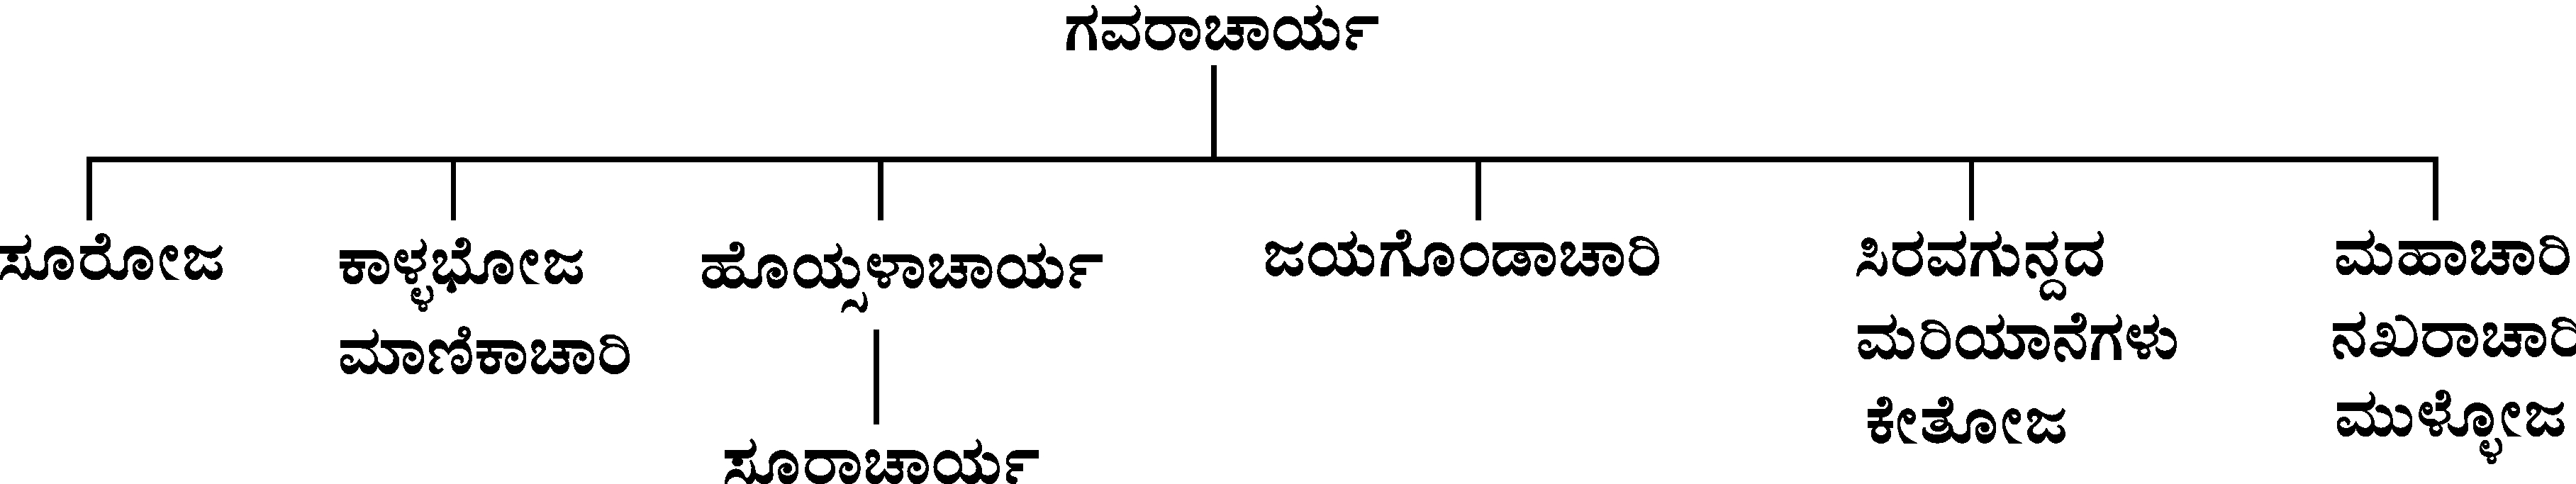
\includegraphics[scale=.92]{"images/chap5/chap5fig4.jpeg"}
\end{figure}

ಸೂರೋಜ, ಕಾಳ್ಳಭೋಜ ಮಾಣಿಕಾಚಾರಿ ಇವರನ್ನು ಸೂರಾಚಾರ್ಯನ ‘ಪಿರಿಯಂಮಂಗಳು’ ಎಂದರೆ\break ದೊಡ್ಡಪ್ಪಂದಿರು ಎಂದೂ, ಜಯಗೊಂಡಾಚಾರಿ, ಸಿರವಗುಂದದ ಮರಿಯಾನೆಗಳು ಕೇತೋಜ ಮತ್ತು ಮಹಾಚಾರಿ ನಖರಾಚಾರಿ ಮುಳ್ಳೋಜ ಇವರುಗಳನ್ನು ಸೂರಾಚಾರ್ಯನ ‘ಕಿರಿಯೈಯಗಳು’ ಅಂದರೆ ಚಿಕ್ಕಪ್ಪಂದಿರು ಎಂದು ಶಾಸನದಲ್ಲಿ ಕರೆಯಲಾಗಿದೆ. ಕಾಳ್ಳಭೋಜ, ಸಿರವಗುನ್ದದ ಮರಿಯಾನೆ, ಮಹಾಚಾರಿ ನಖರಾಚಾರಿ ಎಂಬುದು ಇವರ ಬಿರುದುಗಳಿದ್ದಂತೆ ಕಾಣುತ್ತದೆ. ಈಗ್ಗೆ 50 ವರ್ಷಗಳ ಹಿಂದೆ ನೋಡಿದಂತೆ ಮಾಳಗೂರಿನಲ್ಲಿ ಒಂದೇ ಒಂದು ಆಚಾರಿಗಳ ಕುಟುಂಬ ಇದ್ದು ಆ ಮನೆಯ ಯಜಮಾನನ ಹೆಸರು ಸೂರಾಚಾರಿಯ ಮಗ ಕಾಳಾಚಾರಿ ಆಗಿತ್ತು. ಕಾಳಾಚಾರಿಯ ಮಗನ ಹೆಸರೂ ಸೂರಾಚಾರಿ ಆಗಿತ್ತು. ಇವರ ಮನೆಯು ಕರ್ಮಟೇಶ್ವರ ದೇವಾಲಯಕ್ಕೆ ಸಮೀಪದಲ್ಲೇ ಇತ್ತು. ಇವರು ಶಿಖೆಯನ್ನು ಬಿಟ್ಟು ಗಂಟುಹಾಕಿಕೊಂಡು, ಹಣೆಗೆ ಗಂಧವನ್ನು ಇಟ್ಟುಕೊಳ್ಳುತ್ತಿದ್ದರು. ಆ ಕುಟುಂಬವೂ ಆ ಊರಿನಿಂದ ವಲಸೆ ಹೋಯಿತು. ಈಗ ಮಾಳಗೂರಿನಲ್ಲಿ ಒಂದೇ ಒಂದು ಆಚಾರಿಗಳ(ಕಂಚುಗಾರರ) ಕುಟುಂಬವೂ ಇರುವುದಿಲ್ಲ.


\section{ವಿಜಯನಗರ ಕಾಲದ ತಾಮ್ರಶಾಸನದ ರೂವಾರಿಗಳು}

\vskip -3pt

ವಿಜಯನಗರ ಸಾಮ್ರಾಜ್ಯದ ಕಾಲದಲ್ಲಿ ರಾಜರು ಹೊರಡಿಸುತ್ತಿದ್ದ ತಾಮ್ರ ಶಾಸನಗಳನ್ನು ಕಂಡರಿಸುವ ಶಿಲ್ಪಿಗಳ ಹುದ್ದೆಯು ವಂಶಪಾರಂಪರ್ಯವಾದ ಹುದ್ದೆಯಾಗಿತ್ತು. ಇವರು ತಮ್ಮನ್ನು ಆಚಾರ್ಯರೆಂದು ಕರೆದುಕೊಂಡಿದ್ದಾರೆ. ಆಸ್ಥಾನ ಶಾಸನ ಕಂಡರಣೆಕಾರರ ಪರಂಪರೆ ಗಂಗರ ಕಾಲದಿಂದಲೇ ಆರಂಭವಾಗಿರಬಹುದು ಎಂಬುದನ್ನು ದೇವರಹಳ್ಳಿ ಶಾಸನದಲ್ಲಿ ಬರುವ ವಿಶ್ವಕರ್ಮಣಾಚಾರ್ಯನ ಉಲ್ಲೇಖದಿಂದ ಊಹಿಸಬಹುದು. ಗಂಗರ ಕಾಲದಲ್ಲಿ ಈ ಪದವಿಯ ಹೆಸರು \textbf{“ವಿಶ್ವಕರ್ಮಾಚಾರ್ಯ”} ಎಂದಿದ್ದರೆ, ವಿಜಯನಗರ ಕಾಲದಲ್ಲಿ \textbf{“ಆಚಾರ್ಯ” }ಅಥವಾ \textbf{“ಶಾಸನಾಚಾರ್ಯ” }ಎಂದಾಗಿದೆ. ಇವರು ವಂಶ ಪರಂಪರೆಯಾಗಿ ಮಲ್ಲಣಾಚಾರ್ಯ ಮತ್ತು ವೀರಣಾಚಾರ್ಯ ಎಂದು ಹೆಸರಿಟ್ಟುಕೊಳ್ಳುತ್ತಿದ್ದರು. ‘ತ್ವಷ್ಟಾ’\endnote{ ಕುಮಾರಸ್ವಾಮಿ, ಡಾ॥ ಕೆ.ಎಸ್​. ಪೂರ್ವೋಕ್ತ, ಪುಟ 132} ಮತ್ತು ‘ಲೇಖಕ’ ಎಂದು ಹೇಳಿಕೊಂಡಿರುವುದರಿಂದ ಶಾಸನಗಳನ್ನು ತಾಮ್ರದ ತಗಡಿನ ಮೇಲೆ ಬರೆಯುವುದು ಮತ್ತು ಕೆತ್ತುವುದು ಎರಡನ್ನೂ ಇವರು ಮಾಡುತ್ತಿದ್ದರೆಂದು ಹೇಳಬಹುದು. \textbf{“ಶಾಸನಾಚಾರ್ಯಧರ್ಮೇಣ ಶಾಸನಂ ಸ್ವಾಮಿ ಶಾಸನಂ”} ಎಂದು ಹೇಳಿರುವುದರಿಂದ, ಇವು ಧರ್ಮಶಾಸನಗಳಾಗಿದ್ದು, ಇದನ್ನು ಬಹಳ ಭಕ್ತಿಯಿಂದ, ನಂಬಿಕೆಯಿಂದ ಇವರು ಬರೆದಿದ್ದಾರೆ (ಕೊರೆದಿದ್ದಾರೆ) ಎಂದು ಹೇಳಬಹುದು. ಈ ಬರೆಯುವ ಕ್ರಿಯೆಯನ್ನು “ಲೇಖ,ಲಿಖಿತ” ಎಂದೇ ಹೇಳಿದೆ. ಮಂಡ್ಯ ಜಿಲ್ಲೆಯಲ್ಲಿ ದೊರಕಿರುವ ವಿಜಯನಗರ ಕಾಲದ ತಾಮ್ರ ಶಾಸನಗಳನ್ನು ಬರೆದಿರುವ ಆಚಾರ್ಯರುಗಳ ಹೆಸರುಗಳು ಈ ಕೆಳಗಿನಂತಿವೆ.

\vskip -2pt

“\textbf{ಶ‍್ರೀ ದೇವರಾಯ ನೃಪತೇಃ ಶಾಸನಮಮ್ಲಾನ ಪಾರಿಜಾತಸ್ಯ। ಶ‍್ರೀ ಶಾಸನಾಚಾರ್ಯ ಧರ್ಮೇಣ ಶಾಸನಂ ಸ್ವಾಮಿ ಶಾಸನಂ। ತ್ವಷ್ಟಾ ವರದಪಾಚಾರ್ಯ ಹಸ್ತೇನ ಲಿಖಿತಂತ್ವಿದಂ”\endnote{ ಎಕ 6 ಶ‍್ರೀಪ 25 ಶ‍್ರೀರಂಗಪಟ್ಟಣ 1430}, }ಎಂದು ಶ‍್ರೀರಂಗಪಟ್ಟಣ ತಾಮ್ರಶಾಸನದಲ್ಲಿ,\textbf{ “ತ್ವಷ್ಟಾ ವರದಾಪಾಚರ್ಯ ಸೂನುಃ ಶಾಸನ ಲೇಖಕಃ ಶ‍್ರೀ ಗಿರಿಸ್ಸುಗುಣೋ ಧೀಮಾನ್ವೃತಿಮೇಕಾಮಿಹಾಶ್ನುತೇ”} ಎಂದು ನೆಲಮನೆ ಶಿಲಾಶಾಸನದಲ್ಲಿ ಹೇಳಿದೆ.\endnote{ ಎಕ 6 ಶ‍್ರೀಪ 93 ನೆಲಮನೆ 1458} ಈ ಶಾಸನಗಳನ್ನು ಕ್ರಮವಾಗಿ ಶಾಸನಾಚಾರ್ಯ ವರದಪ್ಪಾಚಾರ್ಯ ಮತ್ತು ಅವನ ಮಗ ಶ‍್ರೀಗಿರಿ ಇವರು ಕಂಡರಿಸಿದ್ದು, ಇವರದೊಂದು ಶಾಸನಾಚಾರ್ಯರ ಮನೆತನವೆಂದು ಹೇಳಬಹುದು. ಶಾಸನಾಚಾರ್ಯರು ಕೇವಲ ತಾಮ್ರಶಾಸನಗಳನ್ನಲ್ಲದೆ ಶಿಲಾಶಾಸನಗಳನ್ನೂ ಕಂಡರಿಸುತ್ತಿದ್ದರು ಎಂಬುದು ಇದರಿಂದ ತಿಳಿದುಬರುತ್ತದೆ. ಜಿಲ್ಲೆಯಲ್ಲಿ ಸಿಗುವ ವಿಜಯನಗರ ಕಾಲದ ತಾಮ್ರ ಶಾಸನಗಳನ್ನು ಕಂಡರಿಸಿರುವವರ ವಿವರ ಈ ಕೆಳಗಿನಂತಿದೆ.

\vskip -2pt

\textbf{“ತ್ವಷ್ಟಾ ಶ‍್ರೀ ಮುದ್ದಣಾಚಾರ್ಯ ಸೂನು ಶಾಸನ ಲೇಖಕಃ ವೀರಣಃ ಸುಗಣೋ ಧೀಮಾನ್​\general{\break } ವೃತ್ತಿರೇಕಾಮವಾಪ್ತವಾನ್​”\endnote{ ಎಕ 6 ಶ‍್ರೀಪ 21 ಶ‍್ರೀರಂಗಪ್ಪಟಣ 1447}, “ತ್ವಷ್ಟಾ ಸೀ(ಶ‍್ರೀ) ವೀರಣಾಚಾರ್ಯಸೂನುಃ ಶಾಸನ ಲೇಖಕಃ ಮಲ್ಲಣಃ ಸುಗುಣೋಧಿಮಾನ್​ ವೃತ್ತಿಮೇಕಾಮೆಹಾಶ್ನುತೇ”\endnote{ ಎಕ 7 ಮ 1139 ಸುಜ್ಜಲೂರು 1473}, “ಮಲ್ಲಣಾಚಾರ್ಯವರ್ಯ ಶ‍್ರೀ ವೀರಣಾಚಾರ್ಯ ನಂದನಃ ಅಕಲ್ಪ ಮಶ್ನುತೇತ್ರೈಕಾಂ ವೃತ್ತಿಂ ಶಾಸನ ಲೇಖಕ”\endnote{ ಎಕ 7 ನಾಮಂ 134 ದೊಡ್ಡಜಟಕ 1512}, “ತ್ವಷ್ಟಾ ಶ‍್ರೀ ಮಲ್ಲಣಾಚಾರ್ಯ ವೀರಣಾಚಾರ್ಯ ನಂದನಃ ಆಕಲ್ಪನ್ಮಸ್ನುತೇತ್ರೈಕಾಂ ವೃತ್ತಿ ಶಾಸನ ಲೇಖಃ”\endnote{ ಎಕ 7 ಮಂ 1516 ಮಂಡ್ಯ 1516}, “ಅಚ್ಯುತೇಂದ್ರ ಮಹಾರಾಯ ಶಾಸನಾನ್ಮಲ್ಲಣಾತ್ಮಜಃ ತ್ವಷ್ಟಾ ಶ‍್ರೀ ವೀರಣಾಚಾರ್ಯ್ಯೋ ವ್ಯಲಿಖಿತ್ತಾಮ್ರ ಶಾಸನಂ”\endnote{ ಎಕ 6 ಕೃಪೇ 99 ಬ್ಯಾಲದಕೆರೆ 1532}, “ಅಚ್ಯುತ ವಿಹಿತ ವಿಭೋತೇರಚ್ಯುತ ರಾಜಸ್ಯ ಶಾಸನಂ ತದಿದಂ ತಾಮ್ರ ಶಾಸನಂ ಅಚ್ಯುತೇಂದ್ರ ಮಹಾರಾಯ ಶಾಸನಾನ್ಮಲ್ಲಣಾತ್ಮಜಃ ತ್ವಷ್ಟಾ ಶ‍್ರೀ ವೀರಣಾಚಾರ್ಯ್ಯೋವ್ಯ ಲಿಖಿತಂ ತಾಮ್ರ ಶಾಸನಂ”\endnote{ ಎಕ 7 ಮ 144 ಹುರುಗಲವಾಡಿ 1533}, “ಸದಾಶಿವಮಹಾರಾಯ ಶಾಸನಾದ್ವೀರಣಾತ್ಮಜಃ~। ತ್ವಷ್ಟಾ ಶ‍್ರೀ ವೀರಣಾಚಾರ್ಯ್ಯ ವ್ಯಲಿಖತ್ತಾಮ್ರಶಾಸನಂ।”\endnote{ ಎಕ 7 ನಾಮಂ 107 ಹೊನ್ನೇನಹಳ್ಳಿ 1545}} ಈ ಏಳು ತಾಮ್ರ ಶಾಸನಗಳಲ್ಲಿ ಮುದ್ದಣಾಚಾರ್ಯನ ವಂಶವು ಉಲ್ಲೇಖಿತವಾಗಿದೆ. ಇವರೆಲ್ಲರೂ ಕೂಡಾ ಶಾಸನ ಸಭಾಪತಿಗಳಾಗಿ ವಿಜಯನಗರ ಸಾಮ್ರಾಜ್ಯದ ವಿವಿಧ ರಾಜರ ಆಸ್ಥಾನದಲ್ಲಿ ಕಾರ್ಯನಿರ್ವಹಿಸಿದ್ದಾರೆ. ಮೇಲ್ಕಂಡ ಶಾಸನಗಳ ಆಧಾರದಿಂದ ಇವರ ವಂಶವೃಕ್ಷವನ್ನು ಈ ರೀತಿ ಕಟ್ಟಿಕೊಡಬಹುದು.

\begin{figure}[!h]
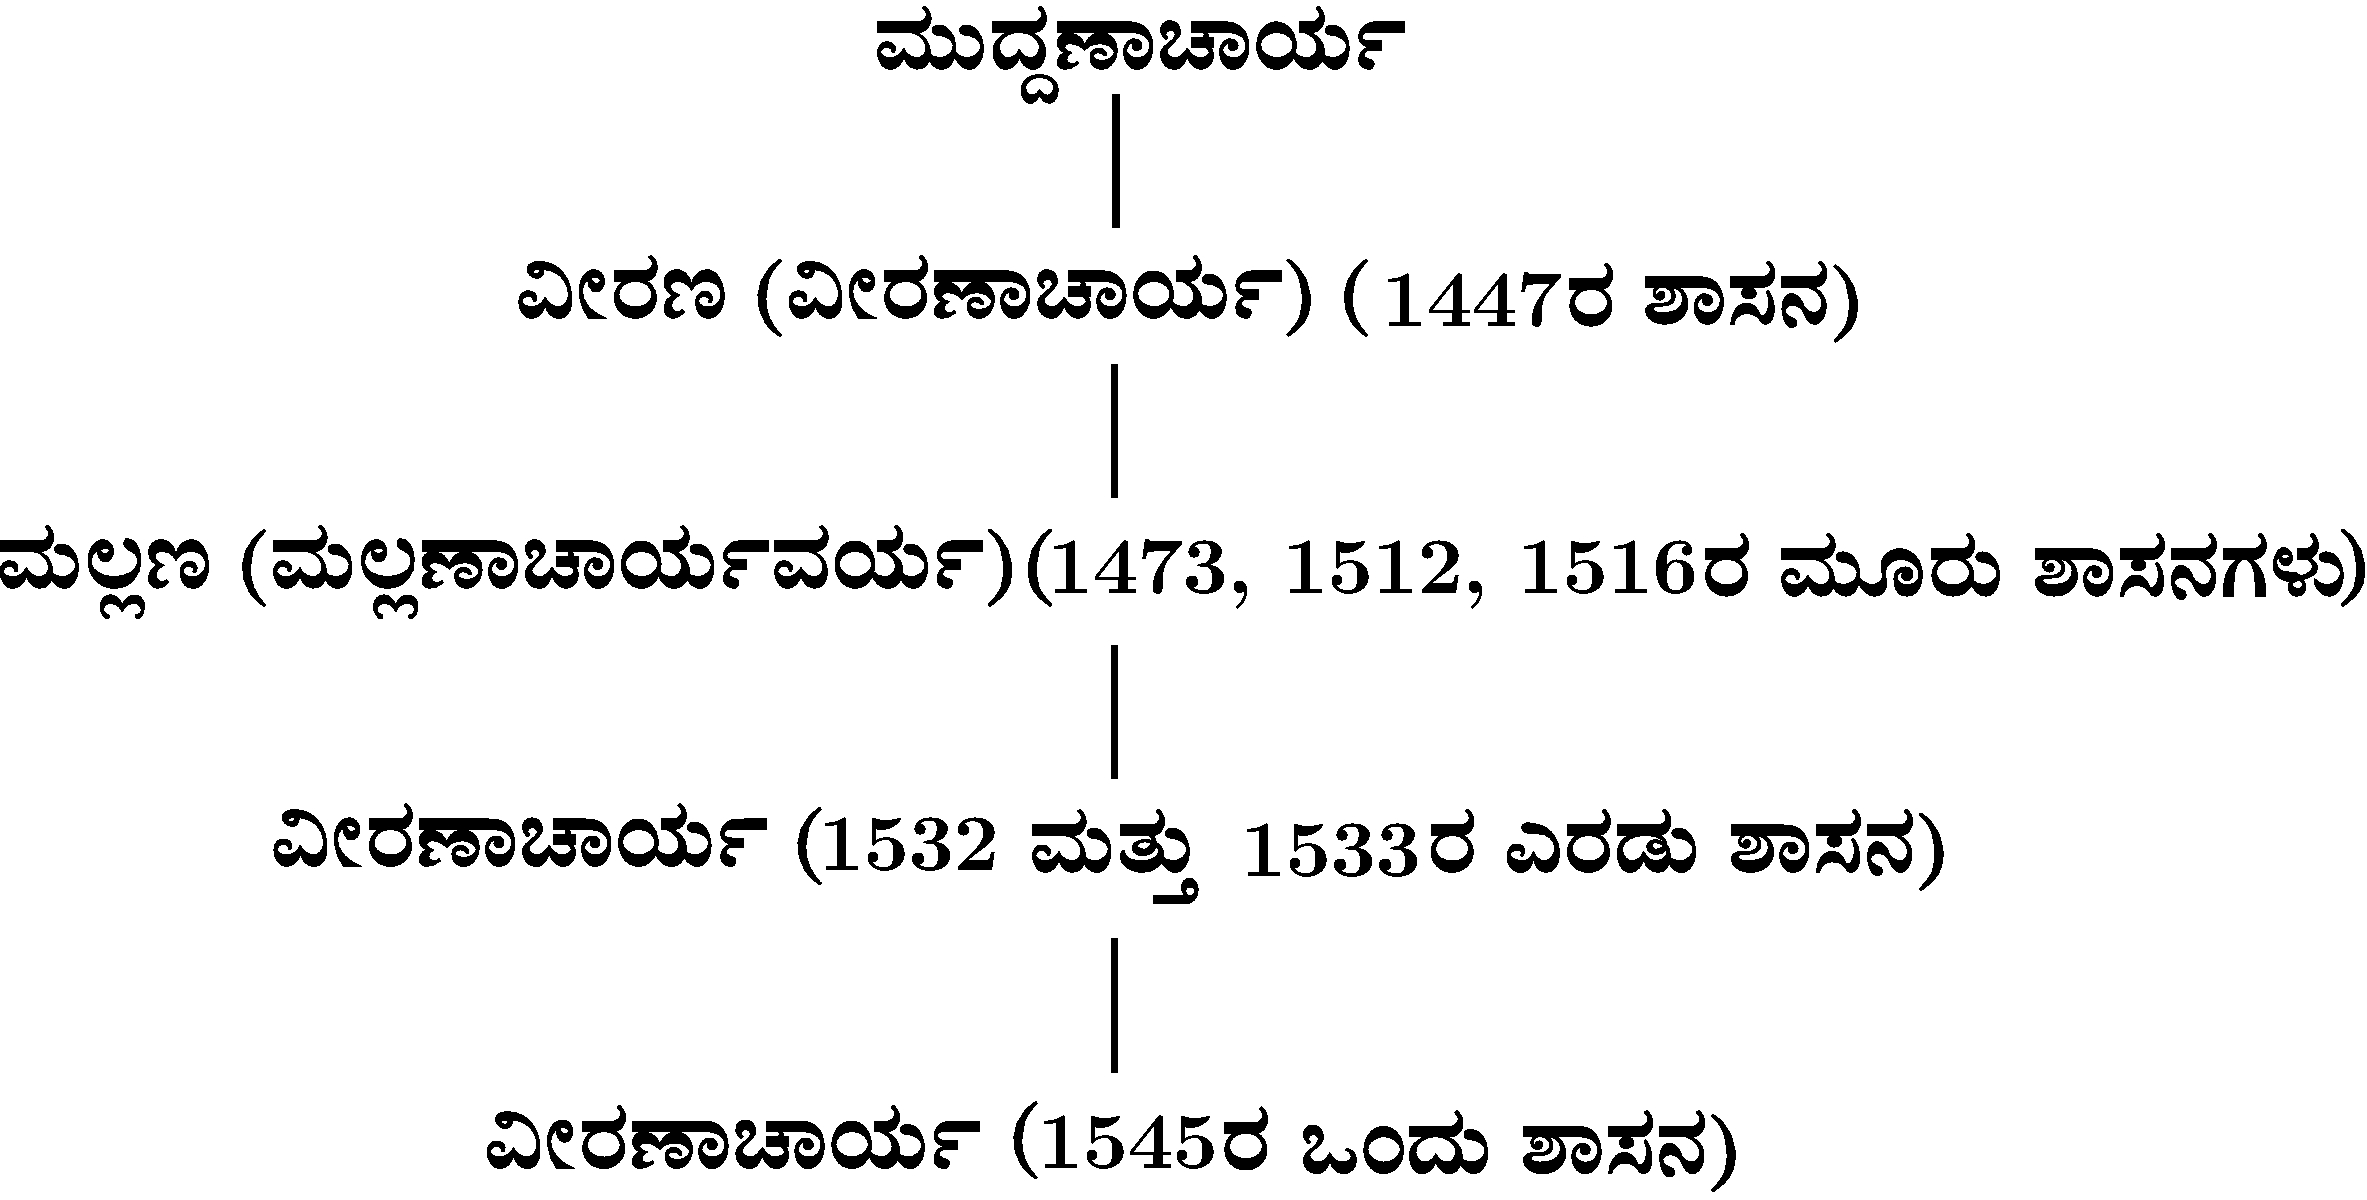
\includegraphics{"images/chap5/chap5fig5.jpeg"}
\end{figure}

ಇವರ ಪೂರ್ಣ ವಂಶವೃಕ್ಷವನ್ನು ವಿದ್ವಾಂಸರು ಕಟ್ಟಿಕೊಟ್ಟಿದ್ದಾರೆ.\endnote{ ಕುಮಾರಸ್ವಾಮಿ, ಡಾ. ಕೆ.ಎಸ್., ಪ್ರಾಚೀನ ಕರ್ನಾಟಕದಲ್ಲಿ ಶಿಲ್ಪಾಚಾರಿಯರು, ಪುಟ 60} ಈ ವಂಶವೃಕ್ಷದಲ್ಲಿ ವೀರಣಾಚಾರ್ಯನ ಮಗ ವೀರಣಾಚಾರ್ಯನಿಗೆ(?) ಪ್ರಶ್ನಾರ್ಥಕ ಚಿಹ್ನೆಯನ್ನು ಹಾಕಿದ್ದು, ಇದರಲ್ಲಿ ಯಾವುದೇ ಅನುಮಾನವಿಲ್ಲ.\endnote{ ಕುಮಾರಸ್ವಾಮಿ, ಡಾ॥ ಎಸ್​.ಕೆ., ಪೂರ್ವೋಕ್ತ, ಪುಟ 57-61} ಇವರೆಲ್ಲರೂ ಶಾಸನವನ್ನು ಬರೆದು ಕಂಡರಿಸಿದ್ದಕ್ಕೆ ಎಲ್ಲ ಕಡೆಯೂ ಒಂದೊಂದು ವೃತ್ತಿಗಳನ್ನು ಪಡೆದಿರುವಂತೆ ಕಂಡು ಬರುತ್ತದೆ. ಒಂದು ಶಾಸನಕ್ಕೆ ಒಂದು ವೃತ್ತಿಯಂತೆ ಇವರು ಪಡೆದಿರುವ ಸಾಧ್ಯತೆ ಇದೆ.


\section{ಸಭಾಪತಿ}

ತಾಮ್ರಶಾಸನಗಳನ್ನು ರಾಜರ ಆಸ್ಥಾನದಲ್ಲಿ ವಂಶಪಾರಂಪರ್ಯವಾಗಿ ಶಾಸನಲೇಖಕರ ಹುದ್ದೆಯನ್ನು ಹೊಂದಿರುತ್ತಿದ್ದ ಲೇಖಕರು ಬರೆಯುತ್ತಿದ್ದರು. ಈ ಹುದ್ದೆಯ ಹೆಸರು ಸಭಾಪತಿ ಎಂದಾಗಿತ್ತು. ಮೃದುಪದ ರಚನೆಯಲ್ಲಿ ಇವರು ಸಿದ್ಧಹಸ್ತರಾಗಿದ್ದರೆಂದು ಶಾಸನದಲ್ಲಿ ಹೇಳಿವೆ. ಇವರು ಬರೆದ ಶಾಸನಗಳನ್ನು ತಾಮ್ರದ ಹಾಳೆಯ ಮೇಲೆ ಕಂಡರಿಸುವ ಕಾರ್ಯವನ್ನು ವಿಶ್ವಕರ್ಮ ಎಂಬ ಹುದ್ದೆಯನ್ನು ಹೊಂದಿದ್ದ ರೂವಾರಿಗಳು ಮಾಡುತ್ತಿದ್ದರೆಂದು ಹೇಳಬಹುದು.

ಕೃಷ್ಣದೇವರಾಯನ ಕಾಲದಲ್ಲಿ “ಸಭಾಪತಿ” ಎಂಬುದು ವಿಜಯನಗರ ಆಸ್ಥಾನದ ಶಾಸನ ಬರಹಗಾರನಾಗಿದ್ದನು. ಶಾಸನದ ಕೊನೆಯಲ್ಲಿ ಲೇಖಕನ ಉಲ್ಲೇಖ ಈ ರೀತಿ ಬರುತ್ತದೆ. \textbf{“ಕೃಷ್ಣದೇವಮಹಾರಾಯ ಶಾಸನೇನ ಸಭಾಪತಿಃ ಉಕ್ತವಾನ್ಮೃದುಸಂದರ್ಭಂ ತದಿದಂ ತಾಂಬ್ರಶಾಸನಂ।”\endnote{ ಎಕ 7 ನಾಮಂ 134 ದೊಡ್ಡಜಟಕ 1512},} ಉಳಿದ ತಾಮ್ರಶಾಸನಗಳಲ್ಲಿ ಸಭಾಪತಿ ಎಂದು ಮಾತ್ರ ಹೇಳಿದೆ. \textbf{“ಕೃಷ್ಣರಾಯಸ್ಯ ಶಾಸನಮುರುಕವಿ ವಿಭವನಿವಹನಿದಾನಸ್ಯ ಭೂರಿ ದಾನಸ್ಯ ಕೃಷ್ಣದೇವಮಹಾರಾಯ ಶಾಸನೇನ ಸಭಾಪತಿಃ ಆಭಾಣೀ ಮೃದು ಸಂದರ್ಭಂ ತದಿದಂ ತಾಂಬ್ರಸಾಸನಂ”\endnote{ ಎಕ 7 ಮಂ 1516 ಮಂಡ್ಯ 1516}, “ಅಚ್ಯುತೇಂದ್ರ ಮಹಾರಾಯ ಶಾಸನೇನ ಸಭಾಪತಿಃ ಅಭಾಣೀನ್ಮೃದುಸಂದರ್ಭಂ ತದಿದಂ ತಾಮ್ರಶಾಸನಂ”\endnote{ ಎಕ 6 ಕೃಪೇ 99 ಬ್ಯಾಲದಕೆರೆ 1532}, “ಮೃದುಪದಮಿತಿ ತಾಮ್ರಶಾಸನಾರ್ಥಂ ಮಹಿತ ಸದಾಶಿವರಾಯಶಾಸನೇನ। ಆಭಣದನುಗುಣಂ ವಚೋ ಮಹಿಮ್ನಾ ಸರಸತರೇಣ ಸಭಾಪತಿ ಸ್ವಯಂಭೂಃ।”\endnote{ ಎಕ 7 ನಾಮಂ 107 ಹೊನ್ನೇನಹಳ್ಳಿ 1545} ಎಂದು ಹೇಳಿದೆ. }ಈ ಶಾಸನದಲ್ಲಿ ಮಾತ್ರ ಸಭಾಪತಿಯ ಹೆಸರು ಸ್ವಯಂಭೂ ಆಗಿರಬಹುದೆಂದು ಊಹಿಸಬಹುದು.

ಜಿಲ್ಲೆಯಲ್ಲಿ ದೊರಕಿರುವ ಕೃಷ್ಣದೇವರಾಯನ ಕಾಲದ ಎರಡು, ಅಚ್ಯುತರಾಯನ ಕಾಲದ ಒಂದು ಹಾಗೂ ಸದಾಶಿವರಾಯನ ಕಾಲದ ಒಂದು ಶಾಸನವನ್ನು ಸಭಾಪತಿ ರಚಿಸಿದ್ದಾನೆ. ಮೆಲ್ಕಂಡ ವಿಶೇಷಣಗಳನ್ನೂ, ಶಾಸನಗಳಲ್ಲಿ ಉಪಯೋಗಿಸಿರುವ ಸಂಸ್ಕೃತ ಅಕ್ಷರ ವೃತ್ತಗಳನ್ನೂ ಗಮನಿಸಿದರೆ, ಇವರು ಸಂಸ್ಕೃತ ಕವಿತ್ವದ ಶಕ್ತಿ ಇದ್ದಿತೆಂದು ಹೇಳಬಹುದು. ಜೊತೆಗೆ ಇವರು ಶಾಸನ ರಚನೆಗಾಗಿ ವೃತ್ತಿಗಳನ್ನೂ ದಾನಗಳನ್ನೂ ಪಡೆದಿರುವುದು ಕಂಡು ಬರುತ್ತದೆ.

\begin{center}
***
\end{center}

\theendnotes

